\documentclass{wits} % loads ukzn.cls
% The class loads legacy bitmap symbol fonts on some TeX installations; disable
% microtype expansion so the document remains portable.
\microtypesetup{expansion=false}
\setlength{\headheight}{15pt}
% Remove blank pages
\let\origcleardoublepage\cleardoublepage
\renewcommand{\cleardoublepage}{\clearpage}

% --- Required packages (only if not loaded in ukzn.cls) ---
\usepackage{lmodern}   % real Type 1 outlines: without it T1 falls back to bitmap fonts
\usepackage{amsfonts,amssymb,amsmath,amsthm,latexsym,tabularx}
\usepackage{bm}             % bold math (\bm) used in the mathematical appendices
% The V9 \volos macro announced test identifiers for tests that did not
% exist. It is superseded by \checkedby in hpformat.sty, which names a test
% in verification/ that runs. The definition is kept only so that any stale
% use is loud rather than silent.
\providecommand{\volos}[1]{\textbf{[stale \texttt{\string\volos} pointer: #1]}}
\usepackage{listings}       % lstlisting environment used in the implementation appendix
% Algorithm packages removed in V2: no algorithm environments are used, and
% requiring them prevented compilation on a standard TeX Live installation.
\usepackage{graphicx}
\usepackage[hidelinks]{hyperref}
\usepackage{makecell,lscape,caption,subcaption,mdframed}
\usepackage{booktabs,float,pdflscape,varwidth,longtable}
\usepackage[round,authoryear]{natbib}
\usepackage{har2nat}   % lets the agsm (Harvard) bibliography style work under natbib
% agsm writes \harvardurl for the URL field; route it through \url so that
% underscores and tildes in web addresses do not break the build.
\usepackage{url}
\renewcommand{\harvardurl}[1]{\textbf{URL:} \url{#1}}
% in preamble:
\usepackage[nonumberlist,acronym,toc]{glossaries}
\makenoidxglossaries
% Load glossary entries
%%%
%\newacronym{eos}{EoS}{Equation of State}  % <- only definitions here
\glsaddall          % make sure all entries appear
\usepackage{tikz}          % Main TikZ package
\usetikzlibrary{arrows}    % For arrow tips
\usetikzlibrary{shapes}    % For custom shapes
\usetikzlibrary{positioning} % For easier node positioning
\usetikzlibrary{calc}      % For calculations
\usetikzlibrary{decorations.pathreplacing} % For braces, decorations
\usetikzlibrary{matrix}    % For drawing matrices/grids
\usepackage{rotating}
\usepackage{array}
\usepackage{hpformat}      % reusable chapter format: roadmap + reading boxes + eq tags
\usepackage{hpresults}     % results from `hpotential thesis-export`; placeholders otherwise




% -----------------------------
% Define custom caption font
% -----------------------------
\DeclareCaptionFont{captionfont}{\fontsize{10pt}{12pt}\selectfont}

% -----------------------------
% Global caption settings for neat multi-line captions
% -----------------------------
\captionsetup{
    font={captionfont,rm},         % 10pt, roman text
    labelfont={bf,rm},             % Bold label, normal case
    textfont=rm,                   % Normal roman text, no italics
    justification=centering,       % Center-align captions
    singlelinecheck=false,         % Center even single-line captions
    margin=0pt,                    % No left/right indent
    width=.85\textwidth,           % Wrap long captions neatly at 85% of text width
    skip=0.5em,                    % Space between figure/table and caption
    format=plain                   % Plain format, no hanging indent
}

\setlength{\parindent}{0pt}


%%
%\newacronym{eos}{EoS}{Equation of State} % Loads your custom commands and glossary definitions.


% =========================================================
% Thesis Meta Data
% =========================================================
% Add the custom \thesislogo command if your ukzn.cls includes it.
% If not, this line should be deleted, and the logo must be added manually.
% Assuming your ukzn.cls is the initial one provided, which DIDN'T have a \thesislogo command,
% but for completeness, if you use the fixed one from the last turn, include this:
%\thesislogo{Thesis Template/Figures/Monochrome-01_1.png}


%%%%%\title{My Amazing Thesis}
%%%%%\author{Joe McStudent}
%%%%%\advisor{Professor Very Important}
%%%%%\coadvisor{Dr. Co-Supervisor}
%%%%%\cocoadvisor{Ms. Co-Co-Supervisor}
%%%%%\submitted{June 2007}




% =========================================================
% Front Matter Content
% =========================================================
\abstractfile{Chapters/abstract.tex}
\prefacefile{Chapters/preface.tex}
\declarationplagfile{Chapters/decl_plagiarism.tex}
\declarationpubfile{Chapters/decl_publication.tex}
\acknowledgementsfile{Chapters/acknow.tex}
\dedicationfile{Chapters/dedication.tex}

\listofabbreviationsfile{Chapters/listofacro.tex}
\listsofsymbolsfile{Chapters/symbols.tex}


\begin{document}
%%\frontmatter


%%\mainmatter
% =========================================================
% Main Chapters
% =========================================================
\chapter{Introduction and Background}
\label{ch:introduction}

\begin{ataglance}[How to read this chapter]
The argument runs in six steps. Living longer is not the same as living well,
so health has to be measured as a capacity exercised in circumstances rather
than as a state recorded at a moment (\S\ref{sec:intro-background}). Several
research traditions each answer part of that question and none answers all of
it (\S\ref{sec:intro-traditions}). A capability reading supplies the missing
bridge between what a body can do and what a life permits
(\S\ref{sec:intro-bridge}), but turning a bridge into a number raises a
measurement problem that most composite indices step over
(\S\ref{sec:intro-measurement}). The response is a small piece of mathematics:
a realisation function derived from stated axioms rather than assembled by
convenience (\S\ref{sec:intro-maths}). What follows from that, and what the
thesis will and will not claim, closes the chapter.

Two people appear throughout the thesis and are introduced in
\S\ref{sec:intro-cases}. Every equation is applied to at least one of them, so
that a reader who prefers clinical reasoning to algebra can follow the argument
through the cases alone.
\end{ataglance}

\section{Background: from disease to health as a capacity-in-context}
\label{sec:intro-background}

The starting point for this thesis is a relatively simple observation: living longer is not the same as living in good health. As populations age and survival with chronic disease improves, the clinically and socially important question increasingly concerns what people are able to retain, recover, or realise over the course of later life. This is not a rejection of disease-based measurement. Disease remains a fundamental determinant of health and an essential object of clinical care. The difficulty arises when disease status is treated as if it were a complete description of health.

The World Health Organization's healthy-ageing framework provides an important conceptual shift. It defines healthy ageing in terms of the development and maintenance of functional ability, and locates that ability in the interaction between an individual's intrinsic capacity and the environment in which the individual lives. Intrinsic capacity refers to the physical and mental capacities available to the person, while the environment includes the social, physical, economic and institutional circumstances that can either enable or constrain their expression \citep{who_2015_ageing,beard_intrinsic_2019}. The importance of this formulation is not simply that it adds ``environment'' to a list of health determinants. It changes the object of measurement. What matters is the extent to which a person's capacities can be turned into functioning that means something to them, and that is a different quantity from the capacities themselves.

This distinction creates a problem for conventional measurement. A diagnosis identifies pathology; a functional measure describes what a person can or does do; a quality-of-life instrument captures aspects of experienced health; a frailty index represents accumulated deficits; and a prognostic model estimates the probability of a future event. These quantities are related, sometimes strongly, but their conceptual equivalence cannot be assumed. Treating them as interchangeable risks producing a score whose statistical coherence conceals conceptual ambiguity.

The problem becomes more consequential in chronic conditions in which improvements in treatment alter survival without eliminating the accumulated consequences of disease. Haemophilia is an important example for this thesis. Contemporary treatment has transformed the prognosis of people with haemophilia, while ageing has introduced a more complex clinical landscape in which joint damage, mobility limitations, treatment burden and psychological wellbeing coexist with age-related multimorbidity \citep{srivastava_2020,mauser_2009}. The health that matters to a person ageing with haemophilia is therefore not exhausted by the presence or absence of bleeding episodes. It includes the capacity to move, participate, maintain relationships, obtain appropriate care and pursue valued activities within the circumstances in which that person lives.

The thesis consequently begins from a narrower and more demanding question than the claim that existing health measures are inadequate. The literature already contains sophisticated approaches to multidimensional health. The question is whether a defensible construct can be developed at the intersection of three traditions that have often been operationalised separately: intrinsic or biomedical capacity, the social conditions that enable the exercise of that capacity, and structural conditions that constrain it.

Before turning to those traditions, it helps to have two people in mind against
whom every later claim can be checked.

\section{Two people this thesis keeps returning to}
\label{sec:intro-cases}

Abstract argument about health measurement is easy to agree with and hard to
test. To keep the argument honest, two people are carried through the whole
thesis. Neither is a real patient; both are composites assembled from the
distributions in the data sources used here. They are introduced now, applied
to every equation as it appears, and revisited in the final chapter.

\begin{ataglance}[Mrs~A, the population case]
Mrs~A is 78, widowed, and lives alone on the second floor of a walk-up flat.
She has knee osteoarthritis, mild cognitive impairment, hypertension and early
chronic kidney disease. She dresses and washes herself but no longer carries
shopping up the stairs. Her income is a state pension. She does not drive; her
clinic is forty minutes away by two buses, and she has missed three of her last
eight appointments. Her daughter telephones daily and visits monthly from
another city.

Mrs~A stands for the population the empirical work actually studies: an older
adult of the kind sampled by the National Health and Aging Trends Study, whose
clinical problems are unremarkable and whose circumstances do most of the work.
She is the case used whenever the question is measurement, prediction or
population comparison.
\end{ataglance}

\begin{ataglance}[Mr~B, the translational case]
Mr~B is 58 and has severe haemophilia~A with a high-titre inhibitor. He has a
target right ankle and a destroyed left knee from bleeds sustained before
prophylaxis was available to him, chronic pain, and the metabolic consequences
of two decades of reduced mobility. He is employed part-time. Whether he
receives emicizumab or on-demand bypassing agents depends on which country he
lives in and which formulary applies to him.

Mr~B stands for the translational question: what happens to a construct built
in one population when it is carried to a disease, a health system and a
funding regime it was not developed in. He is the case used whenever the
question is transportability, treatment effect or the price of a decision.
\end{ataglance}

The two are chosen because they fail in different directions. Mrs~A has modest
biology and hostile circumstances. Mr~B has severe, well-characterised biology
and circumstances that swing between generous and punitive depending on
jurisdiction. A construct that describes only one of them well has not done the
job this thesis sets out.

\section{The intellectual problem: several valid traditions, no automatic synthesis}
\label{sec:intro-traditions}

The measurement of health has evolved through several traditions, each answering a different question. Health-economic measures such as quality-adjusted life-years and disability-adjusted life-years were developed to place health gains and losses on a common scale for decision-making and burden estimation \citep{whitehead_2010}. Health-expectancy measures combine survival with states of health or disability \citep{who_hale_2019}. Patient-reported outcome measures capture experienced health and functioning. Frailty approaches quantify vulnerability through accumulated deficits. Intrinsic-capacity research asks about the physical and mental resources available to an individual. Capability approaches, drawing particularly on the work of Sen and subsequent health-capability scholarship, shift attention from achieved states to the substantive opportunities people have to be and do what they have reason to value \citep{sen_1993,venkatapuram_2011}.

None of these traditions should be dismissed because it does not answer the precise question posed here. Their differences are analytically useful. QALYs and DALYs are designed for valuation and comparison, not to explain how people realise health. Frailty is explicitly concerned with vulnerability and loss of reserve rather than the broader social conditions under which capacity can be exercised \citep{rockwood_mitnitski_2007}. Intrinsic capacity deliberately centres the individual's physical and mental capacities, while recognising their interaction with environment \citep{beard_intrinsic_2019}. Capability measures extend beyond health status, but that broader reach creates an important discriminant-validity problem: a health-capability construct must not become an indistinguishable proxy for general wellbeing \citep{icecap_o,icecap_o_construct}.

Empirical precedents make the novelty problem even more important. The ATHLOS programme demonstrated that multidimensional health can be represented using latent-variable and item-response approaches, drawing on domains including physical functioning, mental health and cognition \citep{caballero_athlos_2017,oberhauser_2016}. Social-vulnerability research has likewise shown that social disadvantage can be represented quantitatively and can carry prognostic information beyond conventional clinical measures \citep{andrew_social_vulnerability_2008,social_vulnerability_share_2014}. More recent healthy-ageing work has continued to demonstrate that intrinsic capacity, functional ability and environmental conditions are empirically connected, while also highlighting unresolved questions about how these constructs should be operationalised \citep{who_2015_ageing}.

The implication is important: the contribution of this thesis cannot simply be that it combines ``biological'' and ``social'' variables. The literature already provides conceptual and empirical precedents for doing so. The contribution must instead be demonstrated through the quality of the theoretical bridge and through empirical tests capable of distinguishing the proposed construct from its closest neighbours.

The bridge has to be built before it can be tested, and the next section builds
it.

\section{From determinants to capability: the proposed bridge}
\label{sec:intro-bridge}

The central conceptual move of the thesis is to distinguish between a determinant of health and a component of health-related capability. Income, education, housing, transport and access to care can influence health without necessarily being equivalent to health. Conversely, intrinsic capacity may be high while opportunities to exercise that capacity are constrained by an inaccessible environment. The same underlying physical capacity may therefore produce very different lived possibilities in different contexts.

This distinction is consistent with the capability approach, but the thesis does not equate health capability with the broader philosophical concept of human wellbeing. Capability theory is concerned with substantive opportunities, whereas health measurement requires a bounded account of what those opportunities mean in relation to health. The WHO framework offers a practical bridge because it explicitly describes functional ability as emerging from intrinsic capacity, environmental characteristics and their interaction \citep{who_2015_ageing}. The proposed construct builds from this relationship but asks whether it can be made sufficiently explicit and measurable to support individual-level statistical inference.

A second bridge is required with social-determinants and life-course research. Social disadvantage is not simply an additional ``risk factor'' to be placed beside age, multimorbidity or cognition. Education, material resources, housing, social relationships and access to services are embedded in cumulative life-course processes and in institutions that distribute opportunities unequally \citep{who_sdh_2008,marmot_2005}. If these conditions are incorporated into a health-capability measure, the thesis must therefore avoid implying that structural disadvantage is a personal deficit. The proposed interpretation is instead that constrained circumstances can reduce the extent to which existing health capacity can be realised.

A third bridge concerns frailty and reserve. Frailty research provides a powerful demonstration that health can be represented as multidimensional vulnerability rather than as a single diagnosis. At the same time, frailty and capability answer different questions. Frailty asks, in broad terms, how vulnerable a person is to adverse stressors; capability asks what the person is able to realise within a given context. The empirical relationship between these constructs is therefore a testable question, not a definitional identity. A successful H-potential measure should correlate with frailty while retaining information that is not reducible to accumulated deficit burden.

These bridges lead to the proposed construct, $H_{\text{potential}}$. It is defined as health-related capability in later life: the combination of biological and functional capacities available to an individual and the enabling or constraining conditions through which those capacities can be realised. The definition is deliberately relational. It does not treat social disadvantage as a biological property, nor does it treat future mortality as part of the definition of health.

A definition, however, is not yet a measurement. Stating that capability is
relational leaves open how one would ever put a number on it, and that is where
most composite health indices quietly go wrong.

\section{The measurement problem}
\label{sec:intro-measurement}

The proposed construct immediately raises a deeper measurement question. Biomedical and functional indicators such as cognition, mobility and limitations in activities of daily living may plausibly be viewed as manifestations of underlying capacities. Social and structural variables such as income, housing and access to care are conceptually different. They may operate as causes, enabling conditions, constraints, or components of a broader construct. It is therefore not defensible simply to place all indicators into a single reflective factor and assume that the resulting statistical object represents health.

This is not a minor technical issue. Recent reviews of intrinsic-capacity measurement have shown that even within the established WHO framework, studies have alternated between reflective and formative interpretations, often without explicitly stating the measurement model. The choice matters because reflective and formative constructs imply different relationships between the latent concept and its indicators, and consequently different approaches to validity and model evaluation \citep{bollen_lennox_1991,jarvis_2003}.

The thesis therefore treats measurement theory as part of the substantive contribution. Biomedical Potential, Social Modifiers and Systemic Burdens are proposed as theoretically distinguishable domains. Their covariance is an empirical hypothesis. A correlated three-factor model is therefore the starting point, not a second-order factor. A higher-order representation will be considered only if the data demonstrate that a common factor is sufficiently dominant and determinate to justify individual scoring. A bifactor or related general-specific representation may be considered as a sensitivity analysis where identification and sample size permit.

This approach also prevents a second form of circularity. If indicators are selected or weighted because they predict mortality, the resulting score may be an effective risk model while no longer representing the theoretical construct from which it was derived. The measurement model must consequently be developed and evaluated before the outcome analysis is used to judge prognostic utility.

Both the definition and the measurement problem point at the same missing
piece: a rule for combining the three domains that can be argued about rather
than merely asserted. The next section supplies it, and shows what goes wrong
without it.

\section{The central mathematical proposition: from heuristic to an axiomatic realisation model}
\label{sec:intro-maths}

The original conceptual expression
\begin{equation}
    H_{\text{potential}}=(L\cdot Q)S-B
\end{equation}
was useful because it made the intended intuition explicit: health potential was conceived as a quantity that could be strengthened or weakened by biological and social conditions. It is not, however, sufficient as an empirical definition.

Read it slowly, because the whole thesis grows out of what is wrong with it.
$L$ is remaining length of life and $Q$ is the quality of that life, so the
product $L\cdot Q$ is the familiar quality-adjusted survival of health
economics: a clinician can read it as ``how many good years does the biology
allow''. $S$ is a multiplier for social conditions, so a value above one says
that a person's circumstances let them do more with the same body and a value
below one says the reverse. $B$ is a burden imposed by the system, subtracted
at the end.

Apply it to Mrs~A. Suppose her biology allows twelve further years at a quality
of $0.7$, giving $L\cdot Q=8.4$ good years. Her isolation and the two-bus
journey to clinic might be scored $S=0.35$, and the burden of an unaffordable
co-payment $B=1.0$. The formula returns $8.4\times0.35-1.0=1.9$. The number is
easy to compute and hard to defend. Why does the social multiplier act on the
whole of $L\cdot Q$ rather than on part of it? Why is $B$ subtracted in the same
units as good years, when it was measured as a payment? And what stops the
arithmetic from returning a negative number, which would be a person with less
than no capability? Nothing in the formula answers these questions, and the
answers are not arbitrary details: they determine who the measure ranks above
whom.

The equation assumes that the terms are commensurable, that social conditions scale biomedical potential multiplicatively, and that structural burden can be subtracted on a common metric. These are substantive assumptions, not mathematical necessities. Neither capability theory nor the healthy-ageing literature establishes them. The equation is therefore retained only as a conceptual heuristic, and the empirical estimator of the latent construct is allowed to emerge from the measurement model.

The central formal contribution of the thesis is to replace that heuristic with a principled object. Chapter~\ref{chap:crf} develops an axiomatic Capability Realisation Function (CRF): rather than assert a formula, it states the properties a realisation measure must satisfy, including non-compensation, and derives the admissible family from them. The primary form, \citep{cobb_douglas_1928}
\begin{equation}
    H(P,S,R)=P\,S^{\alpha}R^{1-\alpha},\qquad R=1-B,\ 0<\alpha<1,
    \label{eq:crf_intro}
\end{equation}
expresses realised potential $H$ as biomedical potential $P=L\cdot Q$ scaled by a non-compensatory combination of social enablement $S$ and structural freedom $R$.

\begin{reading}[What equation \eqref{eq:crf_intro} says, in words]
Realised health capability is what the body makes possible, discounted by the
fraction of that possibility the person's circumstances actually let them
reach. The discount is the term $S^{\alpha}R^{1-\alpha}$, a weighted geometric
average of social enablement and freedom from structural burden. It runs
between $0$ and $1$, so realised capability can never exceed biomedical
potential: the arithmetic cannot invent health the body does not have. The
exponent $\alpha$ says how the two kinds of circumstance are weighted against
each other, and, more importantly, that they are weighted \emph{multiplicatively}
rather than added.

A geometric average is the formal statement of ``a chain is only as strong as
its weakest link''. Multiply by zero on either side and the product is zero.
This is the property an additive index cannot reproduce, and it is the reason
the form was chosen rather than assumed.
\end{reading}

The three coordinates are used by every chapter that follows, so they are
fixed here once.

\begin{definition}[Domain profile]
\label{def:int:profile}
A person's domain profile is the triple
\[
  \mathbf X=(P,S,R)\in[0,1]^3,
\]
in which $P$ is Biomedical Potential, $S$ is Social Modifiers scored as social
enablement, and $R=1-B$ is structural freedom, the complement of Systemic
Burdens. Every coordinate is oriented so that $0$ is the worst attainable value
and $1$ the best. The realisation function \eqref{eq:crf_intro} is then a map
$H:[0,1]^3\to[0,1]$, and realised capability is bounded by the same interval as
its inputs.

\end{definition}

\begin{remark}[Two scales for $P$, and the conversion between them]
\label{rem:int:scales}
Biomedical potential is reported on two scales in this thesis, and the reader
should know which is in use before meeting either.

The \emph{unit scale} of Definition~\ref{def:int:profile} puts $P\in[0,1]$,
normalised within the calibration population. Appendix~\ref{app:mathematical_foundations}
and the empirical chapters use it, because a latent measurement model returns a
relative position and not a quantity of anything.

The \emph{natural scale} puts $P=L\cdot Q$ in quality-adjusted life-years, as
Chapter~\ref{app:crf} does when the realisation function has to meet an
economic evaluation. Here $H$ inherits the units of $P$ and is read in good
years.

The two differ by normalisation alone. Because the enablers enter only through
the bounded multiplier $S^{\alpha}R^{1-\alpha}$, which is invariant to the
scale of $P$, any statement about the \emph{ratio} of two people's realised
capability, and the whole of the gap decomposition, is identical on both. Only
the level changes.

Mrs~A is the worked case for this. On the natural scale, with $P=8.4$ good
years, she realises $3.1$ of them. On the unit scale, with $P=0.55$, she scores
$0.206$. These are the same calculation and the same woman;
$0.206$ is not a number of years and $3.1$ is not a position in a
distribution. Where a figure for her appears later without its scale named,
$0.206$ is the unit-scale value.

Carrying two scales is a cost, not a feature. It is paid because the
measurement model cannot deliver years without an external calibration study
that has not been done, while an economic evaluation cannot use a position in a
distribution. \S\ref{sec:intro-maths} returns to why the thesis refuses to
manufacture the missing calibration.
\end{remark}

The choice matters clinically, and the two running cases show why. Take Mrs~A
first, with biomedical potential $P=8.4$ good years as above. Score her social
enablement at $S=0.35$ (she lives alone, her daughter is three hours away, she
has withdrawn from the church group she used to attend) and her structural
freedom at $R=0.40$ (no car, two buses, missed appointments, a co-payment she
notices). With $\alpha=0.5$ the multiplier is
$\sqrt{0.35\times0.40}=0.37$, and her realised capability is
$8.4\times0.37=3.1$ good years. An additive index that averaged her
circumstances would give $(0.35+0.40)/2=0.375$ and $3.2$ good years. The two
agree, which is exactly the uninformative case: her circumstances are equally
poor on both sides, so no rule for trading them can matter.

Now change one thing. Suppose transport is solved: a community minibus takes
her to clinic, so $R$ rises from $0.40$ to $0.90$, while her isolation is
untouched at $S=0.35$. The geometric form gives
$\sqrt{0.35\times0.90}=0.56$ and realised capability $4.7$ good years; the
additive form gives $0.625$ and $5.3$. The gap has opened, and it opens further
as one term approaches zero. Suppose instead that Mrs~A's daughter dies and she
is left with no informal support at all, $S=0.05$, while the minibus keeps
$R=0.90$. The geometric form returns $\sqrt{0.05\times0.90}=0.21$, so $1.8$
good years. The additive form returns $0.475$, so $4.0$ good years, and would
record her as more than twice as well off as she is. The additive index has
allowed excellent transport to compensate for having nobody. That substitution
is precisely what the non-compensation axiom forbids, and it is why the
functional form is derived rather than picked.

\begin{workedexample}[int:mrsa]{Mrs~A under the geometric rule and the additive rule}
Take $P=8.4$ good years and $\alpha=0.5$, and compare three states of Mrs~A's
circumstances. The question is how far the two rules disagree, and where.

As she is, $S=0.35$ and $R=0.40$. The geometric multiplier is
$\sqrt{0.35\times0.40}=0.374$ and the additive one is $(0.35+0.40)/2=0.375$, so
the two rules return $3.14$ and $3.15$ good years. Neither rule is doing any
work here, because there is nothing to trade.

Give her the community minibus, $R=0.90$. The multipliers separate to $0.561$
and $0.625$, which is $4.71$ good years against $5.25$. Now take the support
away instead, $S=0.05$ with the minibus kept at $R=0.90$. The geometric
multiplier falls to $0.212$ and the additive one only to $0.475$: $1.78$ good
years against $3.99$. The additive rule records her as $2.24$ times as well off
as the geometric rule does, having let transport stand in for having nobody.

\begin{wecode}[Python]
from hpv.crf import contextual_mean, H

P = 8.4
for s, r in ((0.35, 0.40), (0.35, 0.90), (0.05, 0.90)):
    geo = contextual_mean(s, r, rho=0.0)   # the CRF, a geometric mean
    add = contextual_mean(s, r, rho=1.0)   # the additive comparator
    print(f"S={s:.2f} R={r:.2f}: CRF {P * geo:.2f} yr   "
          f"additive {P * add:.2f} yr   overstatement {add / geo:.2f}x")

print(H(0.55, 0.35, 0.40))   # the same profile on the unit scale: 0.2058
\end{wecode}

\weanswer{$3.14$, $4.71$ and $1.78$ good years under the CRF, against $3.15$,
$5.25$ and $3.99$ under the additive rule. At $S=0.05$ the additive rule
overstates Mrs~A by a factor of $2.24$. Asserted by
\texttt{test\_worked\_example\_intro\_mrs\_a\_geometric\_versus\_additive}.}
\end{workedexample}

Mr~B shows the same structure from the other end. His biomedical potential is
poor and well characterised: an inhibitor, a destroyed knee, chronic pain.
Suppose $P=4.0$. In a system that funds emicizumab and staffs a haemophilia
comprehensive-care centre, his structural freedom is high, $R=0.85$, and stable
employment and a partner give $S=0.70$; his realised capability is
$4.0\sqrt{0.70\times0.85}=3.1$, close to the ceiling his biology allows. Move
him to a jurisdiction where bypassing agents are rationed and the nearest centre
is in another province, $R=0.20$, and the same body yields
$4.0\sqrt{0.70\times0.20}=1.5$. Nothing about Mr~B has changed. The formula
attributes the entire difference to the system, which is the claim the thesis
is making and which \S\ref{sec:intro-maths} must therefore be able to defend
rather than assert. This single object does the work the heuristic could not: it proves the biomedical--context complementarity that is the mathematical form of the intersectional \citep{crenshaw_1991,bowleg_2008} claim, decomposes any capability gap exactly into biomedical, social and structural parts, and, through an equity-sensitive population functional and a budget-constrained policy gradient, turns individual capability into an integrated, distribution-aware policy calculation. It is also falsifiable: the chapter pre-specifies the head-to-head tests that would reject or narrow it. The construct's meaning and the CRF's parameters are fixed without reference to the outcomes, so the empirical chapters test the model rather than fit it.

\begin{workedexample}[int:mrb]{Mr~B funded and Mr~B rationed, one coordinate apart}
On the unit scale Mr~B's profile is $(0.30,0.70,0.85)$ where his treatment is
funded and $(0.30,0.70,0.20)$ where it is rationed. His biology and his
household are identical in the two; only $R$ moves.

The CRF returns $H=0.231$ funded and $H=0.112$ rationed, a ratio of $2.06$. In
the good-years units used above, with $P=4.0$, the same two multipliers give
$3.09$ years and $1.50$ years. The exact gap decomposition of
Chapter~\ref{chap:crf} splits the log ratio
$\log(0.231/0.112)=0.723$ into three parts. The biomedical part is
$\log(0.30/0.30)=0$ and the social part is $0.5\log(0.70/0.70)=0$. The
structural part, $0.5\log(0.85/0.20)=0.723$, is the whole of it.

\begin{wecode}[Python]
from hpv.crf import H, gap_decomposition

funded, rationed = (0.30, 0.70, 0.85), (0.30, 0.70, 0.20)
print(H(*funded), H(*rationed), H(*funded) / H(*rationed))

bio, soc, structural, total = gap_decomposition(funded, rationed)
print(f"biomedical {bio:.3f}  social {soc:.3f}  "
      f"structural {structural:.3f}  total {total:.3f}")
\end{wecode}

\weanswer{$H=0.231$ funded and $0.112$ rationed, a ratio of $2.06$. The
decomposition puts $0.723$ of a total of $0.723$ on the health system and
nothing on Mr~B. Asserted by
\texttt{test\_worked\_example\_intro\_mr\_b\_funded\_versus\_rationed}.}
\end{workedexample}

This distinction also resolves a potentially serious interpretive problem. A standardised latent factor is not automatically measured in years of healthy life. Unless an external calibration study establishes a mapping between the factor and a time-based health-expectancy scale, $H_{\text{potential}}$ must be reported as a latent score with an explicitly defined direction and uncertainty. The thesis will not infer a ``number of healthy years'' from an arbitrary standardisation.

With the formal object in place, the gap the thesis fills can be stated
precisely rather than gestured at.

\section{Research gap and contribution}

The research gap is therefore not the absence of multidimensional health measurement. It is the absence of sufficiently interrogated evidence that a bounded health-capability construct integrating intrinsic capacity with enabling and constraining context can be distinguished empirically from the constructs that surround it.

This gap has four parts. First, the conceptual boundaries between intrinsic capacity, functioning, capability, frailty and social vulnerability \citep{andrew_social_vulnerability_2008} require explicit specification. Second, the measurement model must distinguish variables that plausibly manifest an underlying construct from variables that may instead form or condition it. Third, the proposed construct must demonstrate discriminant and incremental validity against strong comparators. A statistically significant association is not enough. Fourth, if the measure is intended to be equity-sensitive, its meaning and performance must be examined across relevant social groups rather than assuming measurement equivalence.

The central contribution of the thesis is the axiomatic Capability Realisation Model and the integrated policy calculation built upon it (Chapter~\ref{chap:crf}). This is what distinguishes the work from prior multidimensional health measurement: not another weighted index, but a realisation function derived from stated axioms, in which non-compensation, biomedical--context complementarity, an exact capability-gap decomposition, and an equity-sensitive, budget-constrained policy gradient are theorems rather than assertions. The measurement and prognostic work that follows is the empirical test of this model: the outcome-independent latent score provides the domain inputs and the comparator against which the realisation model is judged head-to-head, and the haemophilia chapter shows how the same model travels to a specific disease. The gap the thesis fills is thus the absence of a falsifiable, distribution-aware formal model that turns the intuition of health-as-capability-in-context into individual capability estimates and the policy calculations that follow from them.

The empirical contribution is therefore conditional. If the analyses show that the proposed domains have coherent measurement properties, retain distinguishable substantive meanings, and provide information beyond established measures, and if the realisation model meets its pre-specified head-to-head criteria, then the thesis will have demonstrated a useful bridge between previously separated literatures. If the data do not support those claims, the appropriate conclusion will be that the proposed synthesis is not empirically justified in the present population and that the theoretical framework requires revision. That possibility is not a failure of the research design; it is a necessary feature of an interrogable scientific hypothesis.

The aim and objectives below convert that gap into work that can actually be
carried out.

\section{Aim and objectives}

The overarching aim is to develop an axiomatic model of health-related capability in later life, the Capability Realisation Model, together with the integrated, equity-sensitive policy calculation built upon it, and to evaluate that model empirically using nationally representative longitudinal data from the National Health and Aging Trends Study (NHATS \citep{kasper_2021}).

The specific objectives are to:
\begin{enumerate}
    \item develop a theoretically grounded account of health-related capability by connecting healthy ageing, intrinsic capacity, capability theory, frailty, and social-determinants and life-course research;
    \item derive, from stated axioms, a Capability Realisation Function that specifies how biomedical potential, social enablement and structural freedom combine into realised capability, and build on it an exact capability-gap decomposition, a budget-constrained policy gradient, and an equity-sensitive population functional;
    \item specify and compare competing measurement models for Biomedical Potential, Social Modifiers and Systemic Burdens;
    \item assess construct validity, reliability, factor determinacy and measurement invariance before prognostic modelling;
    \item evaluate the prospective relationship of the resulting domain scores and, only where justified, a higher-order score with five-year all-cause mortality and first unplanned hospitalisation;
    \item determine whether the proposed construct adds information beyond pre-specified measures of frailty, health status and social vulnerability, and test the Capability Realisation Model head-to-head against an additive composite and the outcome-independent factor score on calibration, discrimination and net benefit \citep{vickers_elkin_2006}, with its parameters frozen without reference to the outcomes; and
    \item examine the translational relevance of the framework to ageing with haemophilia, while clearly distinguishing conceptual transferability from disease-specific validation.
\end{enumerate}

\section{Research questions and hypotheses}

The primary research question is:
\begin{quote}
Can a theoretically specified construct of health-related capability, integrating intrinsic and functional capacity with enabling and constraining social context, be measured reliably and validly in later life without collapsing into an existing measure of health status, frailty, social vulnerability or general wellbeing?
\end{quote}

The secondary questions are whether the proposed domains form a coherent but distinguishable structure; whether a higher-order representation is empirically warranted; whether the resulting measure demonstrates incremental prognostic information for mortality and hospitalisation; whether its measurement properties are stable across major demographic and socioeconomic groups; and whether domain-level profiles provide information that is lost when the construct is represented by a single score.

The hypotheses are intentionally stated at the level that the literature and design can support:
\begin{itemize}
    \item \textbf{H1:} Indicators specified within each theoretical domain will demonstrate adequate within-domain measurement coherence, while the domains will remain empirically distinguishable.
    \item \textbf{H2:} A general health-capability factor will be supported only if a higher-order or general-specific model demonstrates sufficient fit, factor determinacy and substantive interpretability relative to the correlated-domain alternative.
    \item \textbf{H3:} The proposed construct will demonstrate incremental prognostic information beyond pre-specified conventional health and frailty measures, assessed using effect estimates, discrimination, calibration and appropriate measures of reclassification or decision utility where justified.
    \item \textbf{H4:} The measurement model will demonstrate adequate invariance across major demographic and socioeconomic groups; where full invariance is not supported, the nature and consequences of non-invariance will be explicitly reported rather than assumed away.
    \item \textbf{H5:} Domain-level profiles will contain clinically or substantively relevant information that is not fully represented by a single higher-order score.
    \item \textbf{H6:} The non-compensatory Capability Realisation Model will separate profiles that an additive composite cannot, and will meet its pre-specified head-to-head criteria, showing no worse calibration or prediction error than the additive and factor-score alternatives and either improved net benefit or clearer detection of structural bottlenecks, with $\alpha$, $\rho$ and the normalisation bounds frozen without reference to the outcomes.
\end{itemize}

\section{Why NHATS provides a useful test of the proposition}

NHATS is appropriate for this research because it was designed to characterise functioning in later life and follows a nationally representative sample of older adults over time. Its combination of self-reported functioning, performance-related measures, health conditions, social circumstances and longitudinal outcomes provides an unusually suitable setting in which to test whether biological capacity and context can be represented jointly.

The use of NHATS also imposes methodological obligations. The sample is not a simple random sample: inference must account for the survey's sampling structure, weights, clustering and strata, and longitudinal analyses require appropriate attention to cohort construction and weighting. The thesis will therefore treat survey design as part of the estimand and inferential framework rather than as a technical correction applied at the end of the analysis. This is particularly important because the purpose of the study is not merely to obtain a good-fitting model in the observed sample, but to make defensible statements about the population represented by NHATS.

NHATS supplies the test bed for Mrs~A. Mr~B has no comparable cohort, which is
why the haemophilia work is presented as a proposed translation rather than a
completed validation, and why the two are kept apart in the chapter ordering
set out next.

\section{A reader's glossary: the same idea in two languages}
\label{sec:intro-glossary}

This thesis is written for three readerships that do not share a vocabulary.
Clinicians, health economists and statisticians each have a name for most of
the ideas used here, and the names are different. Table~\ref{tab:bilingual}
pairs them, so that a term met later in an unfamiliar form can be looked up
rather than guessed at. Each pairing is introduced again in the text at the
point where it first matters; the table is for reference, not instruction.

The pairings are not exact synonyms. They are close enough that a reader who
understands one side will not be lost on the other, which is all a glossary can
honestly do.

\begin{table}[htbp]
\centering
\caption{Quantitative terms and their clinical counterparts, as used in this thesis.}
\label{tab:bilingual}
\footnotesize
\renewcommand{\arraystretch}{1.25}
\begin{tabular}{p{3.3cm} p{3.9cm} p{6.2cm}}
\toprule
\textbf{Quantitative term} & \textbf{Clinical counterpart} & \textbf{What both are naming} \\
\midrule
Endogeneity & Confounding by indication & The exposure was chosen because of something that also affects the outcome. \\
\addlinespace
Attenuation bias & Regression dilution & Measuring the predictor with error pulls its estimated effect towards no effect. \\
\addlinespace
Shrinkage & Regression to the mean & An extreme estimate from sparse information is pulled back towards the average. \\
\addlinespace
Censoring & Alive at last contact & The person's later fate is unknown, which is information, not a missing value. \\
\addlinespace
Competing risk & An event that ends the follow-up & Death removes a person from being at risk of the admission you were counting. \\
\addlinespace
Immortal time & A window where the event could not occur & The design guarantees survival over an interval, and the guarantee looks like benefit. \\
\addlinespace
Discrimination & Ranking patients correctly by risk & Whether the sicker of any two patients gets the higher score. \\
\addlinespace
Calibration & Whether a stated 10 per cent means one in ten & Whether the predicted probabilities are the observed frequencies. \\
\addlinespace
Incremental value & Does this change management? & Whether the new measure adds anything to the one already in use. \\
\addlinespace
Discriminant validity & Is this troponin measured a second way? & Whether two instruments are the same thing under different names. \\
\addlinespace
Reflective indicators & Symptoms of one underlying disease & Tiredness, cold intolerance and dry skin as effects of a low thyroid. \\
\addlinespace
Formative indicators & Ingredients of a risk score & Age, blood pressure, lipids and smoking, which need not correlate. \\
\addlinespace
Latent variable & A quantity inferred, never measured & Glomerular filtration rate behind creatinine and cystatin~C. \\
\addlinespace
Identification & Telling a blocked patient from a choosing one & Whether the data can distinguish the explanations of the same behaviour. \\
\addlinespace
Non-compensation & A chain is as strong as its weakest link & Cardiac output cannot rescue a haemoglobin of two. \\
\addlinespace
Elasticity of substitution & How far one thing stands in for another & Whether good support can make up for a system that will not treat you. \\
\addlinespace
Opportunity cost, $\lambda$ & Patients you never meet & The health lost elsewhere when this budget is spent here. \\
\addlinespace
Inequality aversion, $\varepsilon$ & How much a gain to the worst-off counts & The exchange rate between total health and its distribution. \\
\addlinespace
Net benefit & Finding a case against over-treating & The trade a clinician makes at a chosen decision threshold. \\
\addlinespace
Internal validation & The model marking its own homework & How much of the apparent performance will survive a new sample. \\
\bottomrule
\end{tabular}
\end{table}

With the vocabulary settled, the order of the argument can be set out.

\section{The structure of the thesis}

The remainder of the thesis follows the logic of the argument rather than the chronology of the statistical analysis. Chapter~\ref{ch:literature} develops the literature and establishes the conceptual bridges on which the proposed construct depends. Chapter~\ref{chap:validation} formalises the construct and addresses the measurement assumptions underlying its mathematical representation. Chapter~\ref{chap:crf}, the formal heart of the thesis, develops the axiomatic Capability Realisation Model and the integrated policy calculation built upon it. The following chapters are its empirical test: they describe the NHATS data, variable construction and analytical strategy, present the measurement results, and evaluate prognostic performance and comparative validity, including the head-to-head comparison of the realisation model with an additive composite and the outcome-independent factor score. The validation and sensitivity analyses then examine robustness, equity and alternative specifications. The final chapter returns to the literature and asks what the empirical evidence permits the thesis to claim, what it does not permit it to claim, and what further work is required for disease-specific validation in ageing with haemophilia.

\section{Conclusion}

The thesis is built around a proposition rather than a predetermined index: that health-related capability may be understood as the capacity available to an individual together with the conditions through which that capacity can be realised. The literature provides strong foundations for each part of this proposition, but it does not establish that they should be collapsed into a single empirical construct. That is precisely the question the thesis must test.

The scientific contribution will therefore depend less on the novelty of the ingredients than on the strength of the connection between them. The literature review must show why the domains belong in the same conceptual conversation; the measurement analysis must test whether they can be represented coherently; the prognostic analysis must test whether the resulting construct matters prospectively; and the sensitivity and equity analyses must test whether the interpretation survives reasonable alternatives. At every stage, the code should interrogate the claims, not reproduce them. The thesis will be strongest if the data are allowed to narrow, modify or reject the proposed construct where the evidence requires it.


\chapter{Theoretical Framework and Literature Review}\label{ch:literature}
% Chapter 2 revised: critical literature synthesis, August 2026
\label{ch:theory}

\begin{ataglance}[The argument in outline]
This chapter sets out the theoretical framework. It builds on the literature reviewed in Chapter~\ref{ch:introduction} in seven steps.
\begin{enumerate}\setlength{\itemsep}{2pt}
\item \emph{Build the bridge} from determinants of health to health-related capability, and introduce two illustrative profiles used to check the argument.
\item \emph{Set out the field as a taxonomy.} Five ontological traditions each answer a different question about what ``health'' names (Table~\ref{tab:taxonomy}).
\item \emph{Choose an ontology.} Two candidates, capacity-ceiling and relational, differ on whether context can only convert existing capacity or can also create it.
\item \emph{State the identification problem.} Observed functioning cannot tell a free choice from a blocked one, so capability must be modelled from capacity and context, not read off behaviour.
\item \emph{Place the construct in economics and policy,} where the temptation to overclaim is strongest.
\item \emph{Replace the heuristic formula} with a realisation function derived from stated axioms.
\item \emph{End in falsifiable propositions,} not a declaration of validity.
\end{enumerate}
\end{ataglance}

\noindent
The central problem addressed in this chapter is not whether health is multidimensional. That proposition is well established. Nor is it whether health can be represented by a composite score. The literature contains several successful examples of multidimensional measurement, including the Global Burden of Disease framework, health-expectancy measures, frailty indices, intrinsic-capacity measures, capability measures and latent health metrics developed through factor analysis and item-response theory. The more difficult question is what is gained, and what is lost, when these traditions are brought together in a single construct intended to represent an individual's health-related potential rather than a current health state, a count of deficits, or a probability of an adverse event.

Chapter~\ref{ch:introduction} reviewed five bodies of scholarship: (i) health-state and health-loss measurement; (ii) frailty and deficit accumulation; (iii) the WHO healthy-ageing and intrinsic-capacity framework; (iv) capability theory and capability measurement; and (v) social determinants and social vulnerability. The purpose of bringing these traditions together is not to imply that they are interchangeable. On the contrary, their differences provide the theoretical problem that the thesis must resolve. If intrinsic capacity describes what an individual is able to draw upon, functional ability describes what is realised in context, capability describes the opportunity to achieve valued states and activities, and social vulnerability describes accumulated exposure to social disadvantage, then a proposed health-capability construct must specify precisely where it sits among these concepts.

This leads to a deliberately restrictive claim. The $H_{\text{potential}}$ is not proposed as the first multidimensional health measure, the first latent health score, or the first measure to incorporate social conditions. ATHLOS, for example, constructed a longitudinal health metric using exploratory and confirmatory factor analysis followed by Bayesian multilevel item-response theory, while the WHO framework explicitly links intrinsic capacity, environment and functional ability. \citep{caballero_athlos_2017,who_2015_ageing,who_healthy_ageing_2026} Capability measures such as ICECAP-O likewise demonstrate that capability can be operationalised at the individual level, although the measure is intentionally broader than health. \citep{icecap_o,icecap_o_validation} The proposed contribution is narrower: to test whether a health-bounded construct can explicitly connect biological and functional capacity with enabling social conditions and structural constraints, and whether that construct remains empirically distinguishable from established measures of intrinsic capacity, frailty, social vulnerability and current health.

The chapter consequently ends not with a declaration that the proposed construct is valid, but with a set of propositions that the empirical work must attempt to falsify. The logic is important. A thesis of this kind is strongest when the data are allowed to demonstrate that the proposed construct is unnecessary, multidimensional without a valid general factor, or prognostically redundant. The objective is not to protect the proposed index from such findings but to determine what the evidence can legitimately support.

\section{From determinants to capability: the proposed bridge}
\label{sec:intro-bridge}


The central conceptual move of the thesis is to distinguish between a determinant of health and a component of health-related capability. Income, education, housing, transport and access to care can influence health without necessarily being equivalent to health. Conversely, intrinsic capacity may be high while opportunities to exercise that capacity are constrained by an inaccessible environment. The same underlying physical capacity may therefore produce very different lived possibilities in different contexts.

This distinction is consistent with the capability approach, but the thesis does not equate health capability with the broader philosophical concept of human wellbeing. Capability theory is concerned with substantive opportunities, whereas health measurement requires a bounded account of what those opportunities mean in relation to health. The WHO framework offers a practical bridge because it explicitly describes functional ability as emerging from intrinsic capacity, environmental characteristics and their interaction \citep{who_2015_ageing}. The proposed construct builds from this relationship but asks whether it can be made sufficiently explicit and measurable to support individual-level statistical inference.

A second bridge is required with social-determinants and life-course research. Social disadvantage is not simply an additional ``risk factor'' to be placed beside age, multimorbidity or cognition. Education, material resources, housing, social relationships and access to services are embedded in cumulative life-course processes and in institutions that distribute opportunities unequally \citep{who_sdh_2008,marmot_2005}. If these conditions are incorporated into a health-capability measure, the thesis must therefore avoid implying that structural disadvantage is a personal deficit. The proposed interpretation is instead that constrained circumstances can reduce the extent to which existing health capacity can be realised.

A third bridge concerns frailty and reserve. Frailty research provides a powerful demonstration that health can be represented as multidimensional vulnerability rather than as a single diagnosis. At the same time, frailty and capability answer different questions. Frailty asks, in broad terms, how vulnerable a person is to adverse stressors; capability asks what the person is able to realise within a given context. The empirical relationship between these constructs is therefore a testable question, not a definitional identity. A successful H-potential measure should correlate with frailty while retaining information that is not reducible to accumulated deficit burden.

These bridges lead to the proposed construct, $H_{\text{potential}}$, introduced in Chapter~\ref{ch:introduction}. It is defined as health-related capability in later life: the combination of biological and functional capacities available to an individual and the enabling or constraining conditions through which those capacities can be realised. The definition is deliberately relational. It does not treat social disadvantage as a biological property, nor does it treat future mortality as part of the definition of health.

Before the theory is developed, two illustrative profiles are introduced against which each later claim can be checked.

\section{Two illustrative profiles}
\label{sec:intro-cases}

Abstract argument about health measurement is easy to agree with and hard to
test. To keep the argument honest, two people are carried through the whole
thesis. Neither is a real patient or a case study; both are composites assembled from the
distributions in the data sources used here. They are introduced now, applied
to every equation as it appears, and revisited in the final chapter.

\begin{ataglance}[Mrs~A, the population case]
Mrs~A is 78, widowed, and lives alone on the second floor of a walk-up flat.
She has knee osteoarthritis, mild cognitive impairment, hypertension and early
chronic kidney disease. She dresses and washes herself but no longer carries
shopping up the stairs. Her income is a state pension. She does not drive; her
clinic is forty minutes away by two buses, and she has missed three of her last
eight appointments. Her daughter telephones daily and visits monthly from
another city.

Mrs~A stands for the population the empirical work actually studies: an older
adult of the kind sampled by the National Health and Aging Trends Study, whose
clinical problems are unremarkable and whose circumstances do most of the work.
She is the case used whenever the question is measurement, prediction or
population comparison.
\end{ataglance}

\begin{ataglance}[Mr~B, the translational case]
Mr~B is 58 and has severe haemophilia~A with a high-titre inhibitor. He has a
target right ankle and a destroyed left knee from bleeds sustained before
prophylaxis was available to him, chronic pain, and the metabolic consequences
of two decades of reduced mobility. He is employed part-time. Whether he
receives emicizumab or on-demand bypassing agents depends on which country he
lives in and which formulary applies to him.

Mr~B stands for the translational question: what happens to a construct built
in one population when it is carried to a disease, a health system and a
funding regime it was not developed in. He is the case used whenever the
question is transportability, treatment effect or the price of a decision.
\end{ataglance}

The two are chosen because they fail in different directions. Mrs~A has modest
biology and hostile circumstances. Mr~B has severe, well-characterised biology
and circumstances that swing between generous and punitive depending on
jurisdiction. A construct that describes only one of them well has not done the
job this thesis sets out.

\section{What Does It Mean to Measure Health?}

Measurement begins with a construct, not an algorithm. A score can be calculated whenever observations are combined, but calculation does not establish that the resulting quantity corresponds to a meaningful latent attribute. This distinction is particularly important in multidimensional health research because the word \emph{health} is used to describe states, capacities, functionings, opportunities, vulnerabilities and outcomes that occupy different conceptual levels.

The WHO healthy-ageing framework provides an important starting point because it explicitly distinguishes intrinsic capacity from functional ability. Intrinsic capacity refers to the composite of an individual's physical and mental capacities, while functional ability emerges from the interaction between those capacities and relevant environmental characteristics. The environment is defined broadly, including physical, social and policy contexts and the systems and relationships through which people live. \citep{who_2015_ageing,who_healthy_ageing_2026} This formulation prevents a common measurement error: interpreting an observed limitation as evidence that the underlying biological capacity is absent when the observed limitation may instead reflect an environmental barrier.

The distinction can be expressed conceptually, for person $i$, as
\begin{equation}
\boxed{FA_i=f(IC_i,E_i,IC_i\times E_i)},
\label{eq:who_fa_conceptual}
\end{equation}
where $FA_i$ denotes realised functional ability, $IC_i$ intrinsic capacity and
$E_i$ the relevant environment. Equation~\ref{eq:who_fa_conceptual} is a
translation of the WHO conceptual architecture into notation; it is not an
equation estimated or endorsed by WHO. Writing the interaction among the
arguments of $f$ does not assert a linear interaction term, a multiplicative
production function or any particular scale.

\begin{definition}[Functional ability in the WHO framework]
\label{def:lit-fa}
For person $i$, let $IC_i$ denote intrinsic capacity, $E_i$ the relevant
environment and $FA_i$ realised functional ability. The WHO healthy-ageing
architecture, written in the notation of \eqref{eq:who_fa_conceptual}, posits a
function $f$ with
\[
  FA_i=f\bigl(IC_i,E_i,IC_i\times E_i\bigr).
\]
The definition fixes no scale for $IC$ or $E$, no sign for the interaction and
no functional form for $f$. \citep{who_2015_ageing,who_healthy_ageing_2026}
\end{definition}

\begin{assumption}[The interaction is not redundant]
\label{ass:lit-interaction}
In Definition~\ref{def:lit-fa}, $f$ is not additively separable in its first
two arguments: there exist profiles at which
$\partial^2 f/\partial IC\,\partial E\neq0$.
\end{assumption}

Stated as an assumption rather than folded into the definition, because it is
the substantive claim and it can fail. If the cross-partial were zero
everywhere, capacity and environment would contribute independently, the third
argument of $f$ would carry no information, and an additive index would lose
nothing. Everything the thesis goes on to build rests on this assumption being
false, and Chapter~\ref{ch:results2} is where it is put at risk.

\begin{reading}[Why the interaction term is the whole argument]
Strip \eqref{eq:who_fa_conceptual} of the notation and it says three things.
What a person can do depends on their body. It depends on their surroundings.
And, third, it depends on the two together in a way neither explains alone.
The first two are uncontroversial. The third is the claim.

The clinical case for it is easy to state. Two women have identical hip
radiographs, identical grip strength and identical gait speed: the same $IC$.
One lives in a bungalow with a stairlift-free front door and a supermarket
across the road. The other lives on the second floor of a walk-up. Their $FA$
differs, and it differs by more than either the hips or the stairs would
predict separately, because the stairs matter more when the hips are worse.
That excess is $IC_i\times E_i$.

A measure that omits the interaction is committed to saying the stairs cost
every woman the same. They do not, and the cost of pretending they do falls
hardest on the women for whom the answer matters most.
\end{reading}

The conceptual sequence used in this thesis is \citep{who_2015_ageing}
\begin{equation}
\boxed{\begin{aligned}
\text{health conditions}&\longrightarrow\text{intrinsic capacities}
\longrightarrow\text{health-related capabilities}\\
&\longrightarrow\text{functional ability}
\longrightarrow\text{observed outcomes}
\end{aligned}},
\label{eq:conceptual_sequence}
\end{equation}
with environmental and social structures acting across the sequence. The
arrows express theoretical ordering, not identified causal effects.

\begin{definition}[The conceptual sequence]
\label{def:lit-sequence}
The sequence of \eqref{eq:conceptual_sequence} is the ordered chain
\[
  \text{health conditions}\rightarrow IC\rightarrow
  \text{health-related capability}\rightarrow FA\rightarrow
  \text{observed outcomes},
\]
with environmental and social structure acting on every arrow. Each arrow is a
many-to-one map, so information present at one stage need not survive to the
next. The ordering is theoretical: it says which quantity is upstream of which,
and it does not assert an identified causal effect at any arrow.
\end{definition}

Each arrow in \eqref{eq:conceptual_sequence} is a place where information is
lost, and naming the losses is the point of writing the sequence out. Mrs~A's
osteoarthritis is a health condition. Her reduced quadriceps strength and
slowed gait are the intrinsic capacities it produces. Her capability to leave
the flat is what those capacities plus a second-floor walk-up amount to. Her
functional ability is what she in fact does, which is to go out twice a week.
Her observed outcome is a missed clinic appointment recorded in an
administrative dataset.

Reading backwards along that chain is where measurement goes wrong. The missed
appointment is compatible with severe disease, with a difficult journey, or
with a woman who had something better to do. Existing measures mostly sample
the right-hand end of the sequence and infer leftwards. This thesis samples the
left and middle and refuses to infer from behaviour, which is the position the
next equation formalises.

The thesis therefore asks whether underlying health-related potential can be
measured separately from realised function. Its general construct statement is
\begin{equation}
\boxed{H_{P,i}=f(BP_i,SM_i,SB_i)},
\label{eq:hp_general_class}
\end{equation}
where $BP_i$ is biological and functional capacity, $SM_i$ comprises social and
environmental enabling conditions, and $SB_i$ comprises structural and social
barriers. The mapping $IC\rightarrow BP$ is approximate rather than an asserted
equivalence. Likewise, $E\rightarrow(SM,SB)$ separates enabling conditions from
constraints without implying that every environmental variable belongs inside
the construct. Whether social structure is a component, determinant or modifier
is tested through competing specifications.

\begin{definition}[The H-potential construct class]
\label{def:lit-hpclass}
An H-potential representation is any function $f$ of three domain scores,
\[
  H_{P,i}=f\bigl(BP_i,SM_i,SB_i\bigr),
\]
where $BP_i$ is biological and functional capacity, $SM_i$ enabling social and
environmental conditions and $SB_i$ structural and social barriers, as in
\eqref{eq:hp_general_class}. The definition names a class, not a member. It
commits to two claims and no more: that the three domains partition what
matters for health potential, and that they can be measured apart. Choice of
$f$ within the class is the subject of Section~\ref{sec:lit-candidates} and
Chapter~\ref{app:crf}.
\end{definition}

\begin{reading}[What \eqref{eq:hp_general_class} does and does not commit to]
The equation is deliberately almost empty. It names three domains and asserts
that health potential is some function of them. It does not say the function is
addition, or multiplication, or anything else; $f$ is unspecified on purpose,
because choosing its form is a separate argument made in
Chapter~\ref{app:crf} and not smuggled in here.

Two things are being claimed even so, and both can fail. The first is that
these three domains are the right partition: that nothing important about
health potential falls outside biological capacity, social enablement and
structural burden. The second is that they are separable enough to be measured
apart. If the NHATS indicators cannot distinguish social enablement from
structural burden, the partition collapses to two domains and the thesis has to
say so.

Note also what sits outside the equation. There is no time index, so this is a
snapshot; the dynamic version is Appendix~\ref{app:dynamical}. And there is no
outcome on either side, which is the separation the whole design turns on.
\end{reading}

\begin{table}[htbp]
\centering
\caption{Conceptual and empirical roles in the H-Potential argument}
\label{tab:concept_roles}
\small
\begin{tabular}{p{0.22\linewidth}p{0.22\linewidth}p{0.44\linewidth}}
\hline
Concept & Mathematical representation & Empirical role \\
\hline
Intrinsic capacity & $IC$ & Latent or domain-specific capacities; principal clinical predecessor \\
Environment & $E$ & Context, enablement or constraint; not presumed reflective \\
Functional ability & $FA=f(IC,E,IC\times E)$ & Realised capability and functioning \\
Frailty & $F$ & Competing formative/composite construct \\
Social vulnerability & $SV$ & Contextual competitor and possible determinant \\
H-Potential & $H_P=f(BP,SM,SB)$ & Proposed health-bounded construct \\
Mortality & $(T,D)$ & Downstream prognostic outcome, never a defining indicator \\
Hospitalisation & $(T_H,D_H)$ & Downstream outcome with death as a competing event \\
QALY & utility $\times$ survival & Cardinal economic comparator, not a latent-score interpretation \citep{whitehead_2010,drummond2015} \\
Health expectancy & survival/function & Population-level comparator \\
\hline
\end{tabular}
\end{table}

The capability approach provides a second conceptual bridge. Sen distinguishes achieved functionings from the capability to achieve alternative functionings. \citep{sen_1993} This distinction is useful in health because the same observed outcome can arise from different opportunity structures. A person may not participate in an activity because of choice, because of impaired capacity, or because environmental and institutional constraints make participation difficult. A measurement system that observes only achieved functioning can therefore conflate inability with constrained opportunity.

However, the capability approach cannot be imported into health measurement without qualification. Capability is a theory of human freedom and wellbeing, not a ready-made psychometric definition of health. ICECAP-O illustrates this boundary explicitly: it was developed as a measure of capability wellbeing in older people and intentionally extends beyond health states. \citep{icecap_o,icecap_o_validation} Empirical comparisons also suggest that ICECAP-O and direct health measures overlap only partially, particularly in physical functioning. \citep{icecap_o_validation} This is not a weakness of ICECAP-O; it is evidence that capability and health are related constructs with different scopes.

The present thesis therefore uses the term \emph{health-related capability} in a deliberately restricted sense. It refers to the capacity and opportunity to sustain health-related functioning under the biological and social conditions in which an individual lives. It is not intended to measure total human capability, flourishing, life satisfaction or general wellbeing. This boundary is necessary for discriminant validity: if the construct can only be distinguished from general wellbeing by its name, its theoretical specification is inadequate.

A further distinction is required between a latent construct and a prognostic outcome. A score derived from NHATS is not itself future health. It is an estimate of a latent state hypothesised to be associated with subsequent outcomes. Mortality and hospitalisation therefore cannot be used to define the construct without creating circularity. The measurement model must be developed before the prognostic model is evaluated. Prediction is evidence relevant to validity, but prediction alone does not establish construct meaning.

If several conceptions of health are in play, the first task is to lay them out and see which question each answers. The next section does that side by side rather than in sequence, because the differences between them are the argument.

\section{A Taxonomy of Ontological Traditions}

Five ontological traditions define what the word \emph{health} names, and each answers
a different question. To make the gap the thesis addresses precise, they are set out as
a taxonomy rather than a list, alongside the health-economic, social-vulnerability and
capability-wellbeing measures that serve as comparators. Table~\ref{tab:taxonomy}
states, for each, the construct it targets, how it is structurally represented, its
conceptual limit, and the role it plays in the H-potential argument. The point of the
taxonomy is negative: while every entry is well founded for its own question, none
isolates the object the thesis tests, namely health-related capability as biological
capacity converted, or blocked, by enabling and constraining context.

\begin{table}[htbp]
\centering
\caption{A taxonomy of ontological traditions in health measurement, and the role of each in the H-potential argument.}
\label{tab:taxonomy}
\footnotesize
\renewcommand{\arraystretch}{1.15}
\begin{tabular}{p{0.17\linewidth} p{0.17\linewidth} p{0.17\linewidth} p{0.20\linewidth} p{0.20\linewidth}}
\toprule
\textbf{Tradition} & \textbf{Primary construct target} & \textbf{Structural representation} & \textbf{Conceptual limit} & \textbf{Role in the argument} \\
\midrule
Biostatistical naturalism (Boorse \citep{boorse_1977}) & Statistically typical biological function vs a reference class & Species-typical functional norms & Places social context outside health & Fixes the biological pole; motivates $BP$ but is too narrow alone \\
\addlinespace
Action-theoretic holism (Nordenfelt) & Ability to reach vital goals in standard circumstances & Agent-and-goal ability & ``Standard circumstances'' hides structural oppression & Introduces agency; shows why context must be explicit \\
\addlinespace
Capability approach (Sen; Venkatapuram) & Substantive opportunity to achieve valued functionings & Functionings vs the capability set & Broader than health; risks construct conflation & Supplies the capability/functioning distinction, bounded here to health \\
\addlinespace
Deficit accumulation / frailty (Rockwood \citep{rockwood_mitnitski_2007,searle_2008}; Mitnitski) & Accumulated physiological vulnerability & Formative ratio $FI=\sum\text{deficits}/\text{total}$ & Agnostic on cause; omits enabling structures & The competing composite for risk stratification \\
\addlinespace
Intrinsic capacity / healthy ageing (WHO) & Internal physical and mental reserve & Reflective/formative domains & Heterogeneous operationalisation; excludes external context & The biological foundation, $BP$ \\
\midrule
Health-economic summaries (QALY / DALY) & Evaluative preference utility, or disease loss & Composite ratio/interval scale & Evaluates consequences; omits enabling context & Cardinal economic comparator \\
\addlinespace
Social vulnerability & Contextual disadvantage & Composite index of social deficits & Treats context as a personal deficit & Direct contextual competitor \\
\addlinespace
Capability wellbeing (ICECAP-O) \citep{icecap_o,coast_2008} & General human flourishing & Preference-weighted index & Exceeds the health domain & Boundary marker for health-specific freedom \\
\midrule
\textbf{$H_{\text{potential}}$} & Health-related capability in context & Axiomatic non-compensatory realisation function & Requires multi-stage identification and external calibration & The proposed construct \\
\bottomrule
\end{tabular}
\end{table}

\begin{reading}[How to read the taxonomy]
Each row is legitimate for the question it was built to answer; the table is not a
list of failures. Its work is to locate a gap: read down the ``conceptual limit''
column and every established tradition either excludes context, or dissolves the
boundary of health, or treats disadvantage as a personal deficit. The final row is
the thesis's wager that a health-bounded, non-compensatory construct can sit in that
gap, and the rest of the chapter tests whether it can be told apart from its
neighbours.
\end{reading}

A gap in a table is not yet a justification. Whether anything belongs in that
gap depends on what one thinks health is, and on that question the philosophy
of medicine is openly divided.

\section{Rival Philosophies of Health and Their Mathematical Consequences}

The word \emph{health} does not name a philosophically uncontested natural
kind. A naturalist position, associated most prominently with Boorse's
biostatistical theory, locates health in statistically typical biological
functioning relative to an appropriate reference class. Contemporary defences
retain the attraction of separating biological description from judgements
about whether a condition is undesirable. \citep{schwartz_2014_boorse} On this
view, housing, transport, income and institutional access influence welfare and
the consequences of disease, but they are not themselves parts of health.

This position supplies an important objection to H-Potential. If health is
biological functional efficiency, placing social enablement inside a health
score commits a category error. The naturalist model would instead write
\[
H_i^{N}=P_i,
\qquad
FA_i=f(P_i,E_i),
\]
so that $P_i$ measures health and $E_i$ helps explain realised functional
ability. This is a serious comparator, not a straw position. It protects the
medical construct from expanding until every social good becomes health.

Applied to Mr~B, the naturalist reads his health off his factor level, his
joint scores and his inhibitor titre, and says his formulary is a fact about
his country rather than a fact about him. There is something right in that. A
haematologist who recorded ``poor drug funding'' in the problem list alongside
``high-titre inhibitor'' would be making a category error, and a health measure
that let policy failures show up as sickness in the patient would be doing the
same thing at scale. The objection has to be answered rather than waved
through, and the answer this thesis gives is the layered position at the end of
this section: report $P$ separately, always.

Nordenfelt's action-theoretic account moves in a different direction. Health is
connected to a person's ability, under accepted circumstances, to achieve vital
goals. \citep{nordenfelt_1995} This captures something the biological account
misses: intact organs do not guarantee the practical ability to act. Yet it
introduces difficult questions. Which goals are vital? Which circumstances
count as accepted or standard? If an inaccessible environment is treated as
standard, injustice may be normalized; if every adverse circumstance is
incorporated, health risks becoming indistinguishable from general welfare.

Sen's capability approach separates achieved functionings from the real
opportunities to achieve them. \citep{sen_1993} It therefore explains why the
same observed functioning may arise from choice, biological limitation or
constraint. Venkatapuram extends this reasoning by presenting health capability
as a meta-capability shaped by biomedical and social causes and connected to
human dignity and justice. \citep{health_capability_right,venkatapuram_2011}
This supports a relational model in which capability is jointly constituted:
\[
H_i^{R}=G(P_i,S_i,R_i),
\]
without assuming that biomedical capacity is an external ceiling.

The clinical intuition behind the relational reading is also familiar. A person
with paraplegia and a well-fitted wheelchair in an accessible city is not
described by their spinal cord alone; a person with the same lesion, no
wheelchair and no ramps is differently placed in a way that ``same disease,
different circumstances'' does not quite capture. The relational account says
the difference is in their health capability, not merely alongside it.

Daniels provides a further bridge to policy. On a Rawlsian account, protecting
health matters because departures from normal functioning restrict the range of
opportunities open to people; fair health policy must therefore address both
health needs and fair procedures when not all needs can be met.
\citep{daniels_2007} This approach does not imply that one composite score can
settle priority. It makes procedural legitimacy, reasons, revisability and
opportunity effects part of the assessment.

These positions generate two rival ontologies for the thesis. The
\emph{capacity-ceiling ontology} treats $P$ as the maximum potentially
realisable quantity and context as a conversion factor:
\[
H^{C}(P,S,R)=P\,M(S,R),\qquad 0\le H^{C}\le P.
\]
The \emph{relational ontology} permits technology, assistance and institutions
to enlarge effective capability beyond what an unaided capacity measure would
predict:
\[
H^{R}(P,S,R)=G(P,S,R),\qquad H^{R}\not\le P\text{ necessarily}.
\]
Neither is selected by terminology. The ceiling model is more conservative and
clinically anchored; the relational model is more faithful to capability and
disability scholarship. The empirical analysis can examine their consequences,
but fit cannot decide the philosophical question by itself.

\begin{definition}[Capacity-ceiling ontology]
\label{def:lit-ceiling}
Write the profile as $(P,S,R)$ with $R=1-B$. The capacity-ceiling ontology
takes biomedical capacity to be the maximum realisable quantity and context to
be a conversion factor $M:[0,1]^2\rightarrow[0,1]$:
\[
  H^{C}(P,S,R)=P\,M(S,R),\qquad 0\le H^{C}(P,S,R)\le P .
\]
The upper bound is the substantive content. Context can convert capacity that
exists and cannot create capacity that does not, so $P=0$ forces $H^{C}=0$ for
every $S$ and $R$.
\end{definition}

\begin{definition}[Relational ontology]
\label{def:lit-relational}
The relational ontology drops the ceiling. Capability is jointly constituted by
capacity and context through a function $G$,
\[
  H^{R}(P,S,R)=G(P,S,R),
\]
with no requirement that $H^{R}\le P$. Technology, assistance and institutions
may therefore enlarge effective capability past what an unaided capacity
measure predicts, and $P=0$ need not force $H^{R}=0$.
\end{definition}

\begin{reading}[What the two definitions disagree about]
Definitions \ref{def:lit-ceiling} and \ref{def:lit-relational} differ in one
inequality. The ceiling says a wheelchair cannot give a person legs; it can
only let the legs they have carry them further. The relational account says
that a person with a chair, a ramp and a lift is able to do things, and that
being able to do things is what health capability was supposed to mean.

Both are defensible. Neither is chosen here. The thesis carries both, reports
where they diverge, and treats the divergence as a result rather than a
nuisance.
\end{reading}

\begin{reading}[The one case that separates them]
The two ontologies agree almost everywhere and disagree at a boundary. Take a
person with $P$ at or near zero and excellent circumstances. Under the ceiling
model, $H^C=P\,M(S,R)$, and multiplying zero by anything gives zero: their
health capability is nil regardless of the ramps. Under the relational model,
$G$ need not vanish, so their circumstances still count.

Which answer is right is not a question data can settle, because the two
models make identical predictions everywhere else and this corner of the
profile space is sparsely observed. Choosing by fit would mean letting the
distribution of a convenience sample decide a question in the philosophy of
medicine, which is why the thesis carries both and reports where they diverge
rather than picking one and calling the choice a finding.
\end{reading}

The thesis therefore adopts a layered position. Biomedical Potential is
reported as a distinct clinical domain. The multidomain profile is primary.
Scalar aggregation is secondary and conditional. Both ceiling and relational
aggregations are sensitivity models. This prevents a philosophical commitment
from being concealed inside a single equation.

Both ontologies share one difficulty, and it is prior to either of them. Each
treats capability as something a person has. Nobody has ever observed one.

\section{Epistemology: Why Capability Cannot Be Read Directly from Function}

Let $\mathcal C_i$ be the set of health-related functionings genuinely
available to person $i$, and let the achieved functioning be
\[
F_i=\chi_i(\mathcal C_i),
\]
where $\chi_i$ represents choice under the person's information, preferences
and circumstances. It follows that
\[
F_i=F_j\not\Rightarrow\mathcal C_i=\mathcal C_j.
\]
Two people may display the same activity while one had several genuine options
and the other had none. Conversely, non-achievement does not establish
incapability.

\begin{definition}[Achieved functioning map]
\label{def:lit-choicemap}
Let $\mathcal U$ be the set of health-related functionings and let
$\mathcal C_i\subseteq\mathcal U$ be the capability set of person $i$, meaning
the functionings genuinely available to them. The achieved functioning is
\[
  F_i=\chi_i(\mathcal C_i),\qquad \chi_i(\mathcal C)\in\mathcal C ,
\]
where the selector $\chi_i$ represents choice under the person's information,
preferences and circumstances. Only $F_i$ is recorded.
\end{definition}

\begin{theorem}[Observed functioning does not identify the capability set]
\label{thm:lit-identification}
Let $\mathcal C$ range over the non-empty subsets of $\mathcal U$ and let
$\chi$ be a selector in the sense of Definition~\ref{def:lit-choicemap}. If
$|\mathcal U|\ge2$ then $\chi$ is not injective, and consequently
\[
  F_i=F_j\;\not\Rightarrow\;\mathcal C_i=\mathcal C_j .
\]
No function of observed functioning alone recovers $\mathcal C_i$. For any
candidate inverse $g$ with $g(F)\in2^{\mathcal U}$, and any $F$ chosen from $k$
distinct capability sets, $g$ returns the right set for at most one of the $k$
people and is wrong for the other $k-1$.
\end{theorem}

\begin{proof}[Proof sketch]
Take $u\in\mathcal U$ and any two distinct sets $\mathcal C_i,\mathcal C_j$ that
both contain $u$; a selector with $\chi_i(\mathcal C_i)=\chi_j(\mathcal
C_j)=u$ exists whenever $|\mathcal U|\ge2$, so $\chi$ is not injective and the
implication fails. The counting claim follows because $g$ is a function: it
assigns one value to the argument $F$, and that value equals at most one of the
$k$ distinct sets. Identification therefore requires information outside $F$,
which is what Definition~\ref{def:lit-hpclass} supplies by modelling capability
from capacity and context.
\end{proof}

\begin{reading}[What the theorem does not say]
It does not say observed functioning is uninformative. A record of what someone
did is evidence about what they could have done, and in a large sample it
carries a great deal. The theorem says something narrower and harder: the
evidence does not determine the answer, so the gap has to be closed by
assumption, and the assumption has to be stated.

It also sets the price of the alternative. Modelling capability from capacity
and context replaces an unidentified quantity with an estimated one. That is
progress only if the model is written down, published and allowed to fail.
\end{reading}

\begin{reading}[The identification problem, at the bedside]
This is the most consequential piece of algebra in the chapter and it says
something a clinician already knows. Observed behaviour is a choice made from
an opportunity set, and only the choice is recorded.

Three people did not attend the diabetic eye-screening appointment. The first
could not afford the bus. The second was too breathless to travel. The third
read the invitation, weighed it, and decided her cataract surgery next month
made it pointless. The administrative dataset records one variable, DNA, and
$F_i$ is identical for all three. Their opportunity sets $\mathcal C_i$ are
completely different, and so is what should be done about them.

Now run it the other way. Two men both walk four hundred metres. One does it
easily. One does it because he must collect his own medication and has spent
the rest of the day recovering. Same $F$, different $\mathcal C$. Every measure
built on observed functioning, which includes most activities-of-daily-living
scales, is blind to this by construction.

The formal statement $F_i=F_j\not\Rightarrow\mathcal C_i=\mathcal C_j$ is the
reason the thesis models capability from capacity and context rather than
reading it off behaviour. It also states the price: capability is not directly
observable, so it must be inferred, and an inference can be wrong in ways an
observation cannot.
\end{reading}

\begin{workedexample}[lit-identification]{Three people, one recorded outcome}
Three women were invited to diabetic eye screening and none attended. The
dataset records the same value of $F$ for all three: did not attend. Their
capability sets are not the same.

\begin{center}\small
\begin{tabular}{p{0.20\linewidth}p{0.40\linewidth}p{0.28\linewidth}}
\toprule
Person & Capability set $\mathcal C_i$ & Recorded $F_i$ \\
\midrule
No fare & \{home\} & did not attend \\
Breathless & \{home, attend\} & did not attend \\
Informed refusal & \{home, attend, attend and shop\} & did not attend \\
\bottomrule
\end{tabular}
\end{center}

\noindent The sets have one, two and three elements. Theorem
\ref{thm:lit-identification} applies with $k=3$: any rule that reads a
capability set off the record returns one set, so it is right for one woman and
wrong for two. The clinical responses differ completely. The first needs the
fare, the second needs transport and a review of her breathlessness, the third
needs nothing at all.

\begin{wecode}[Python]
sets = {
    "no fare":          frozenset({"home"}),
    "breathless":       frozenset({"home", "attend"}),
    "informed refusal": frozenset({"home", "attend", "attend and shop"}),
}
observed = {name: "home" for name in sets}       # chi_i(C_i), identical
print(len(set(observed.values())), "recorded value(s)")
print(len(set(sets.values())), "distinct capability sets")
for guess in sets.values():
    right = sum(1 for c in sets.values() if c == guess)
    print("a fitted inverse gets", right, "right and", len(sets) - right, "wrong")
\end{wecode}

\weanswer{One recorded value, three distinct capability sets, and any inverse
map is wrong for two of the three. Asserted by
\texttt{test\_theorem\_lit\_choice\_map\_is\_not\_injective}.}
\end{workedexample}

This is an identification problem. Cross-sectional functioning cannot uniquely
recover an unobserved opportunity set. Self-report does not solve it completely
because expectations can adapt to long-standing deprivation, while external
assessment may substitute professional values for those of the person. The
claim made by H-Potential must therefore remain modest: it estimates selected
conditions relevant to health-related opportunity; it does not directly observe
freedom.

The implication for validity is that statistical covariance is insufficient.
Content validation must include clinicians, patients and affected communities;
the indicators must be checked against what people have reason to value; and
discordance between observed functioning, reported opportunity and structural
conditions must be studied rather than averaged away.

With the conceptual and epistemic ground laid, and the measurement traditions
reviewed in Chapter~\ref{ch:introduction}, the question becomes what such a
measure could legitimately be used for. The economics is where the temptation
to overclaim is strongest.

\section{Economic Interpretation: Value, Opportunity Cost and Distribution}

H-Potential is not an economic evaluation outcome. A QALY combines time and
preference-based health-state value; a budget-impact analysis measures
affordability; cost-effectiveness compares incremental costs and consequences.
An H-Potential score has none of these meanings by construction. In particular,
the latent scale does not support a cost-per-H-Potential-unit threshold.

The economic relevance instead lies in diagnosis and heterogeneity. Suppose an
intervention $a$ changes the profile from $X_i(0)$ to $X_i(a)$ at cost $C_i(a)$.
Its profile effect is
\[
\Delta X_i(a)=X_i(a)-X_i(0),
\]
and a scalar effect $\Delta H_i(a)$ is calculated only under a declared
aggregator. Economic evaluation must then compare intervention costs and
established consequences, while asking who gains and which constraint is
changed. A treatment may raise $P$; accessible transport may raise $S$; removal
of financial barriers may raise $R$. Equal total effects can therefore imply
different budgets, responsible agencies and policy mechanisms.

\begin{reading}[Why the profile effect is kept as a vector]
Three interventions produce the same $\Delta H$ of $+0.05$ for Mrs~A. A knee
replacement raises $P$. A befriending scheme raises $S$. Waiving her clinic
co-payment raises $R$. A scalar records all three as identical and hands the
decision-maker no information at all.

The vector $\Delta X$ records them as $(+0.05,0,0)$, $(0,+0.05,0)$ and
$(0,0,+0.05)$, and the three go to different budgets. The first is an
orthopaedic list with an eighteen-month wait. The second is a local-authority
grant of a few hundred pounds. The third is a line in a finance director's
spreadsheet and costs almost nothing to change. Equal capability effects,
utterly unequal in cost, in who is responsible, and in how long they take.

This is the practical reason the framework refuses to collapse the profile.
Not because a scalar is philosophically impure, but because the scalar deletes
the only column a commissioner can act on.
\end{reading}

Opportunity cost remains unavoidable. Funding an intervention displaces other
health-producing activity. H-Potential cannot make that displaced health
disappear and must not be used as a moral multiplier attached after a
cost-effectiveness result. If allocation is considered, the minimum economic
record includes incremental cost, QALYs or another justified consequence,
budget impact \citep{sullivan_2014}, displaced activity, uncertainty and the distribution of gains
and losses.

Distributional cost-effectiveness analysis provides the closest established
economic bridge. It extends conventional evaluation by estimating how health
and opportunity costs are distributed across equity-relevant groups and by
making inequality judgements explicit. \citep{asaria_2016_dcea} H-Potential
profiles could help describe baseline constraints or intervention mechanisms,
but should not replace DCEA's health-opportunity-cost accounting. Nor should a
low score automatically generate priority: doing so could favour interventions
with little benefit, penalise those whose capability is difficult to measure or
double-count disadvantage already included in an equity analysis.

Three distinct economic uses must therefore be separated:
\begin{enumerate}
 \item \emph{descriptive use}: identify the domain in which capability is
 constrained;
 \item \emph{stratified evaluation}: estimate costs and outcomes separately
 for relevant profile groups;
 \item \emph{allocative use}: apply explicit social value judgements through
 a legitimate appraisal process.
\end{enumerate}
Only the first is supported by construct validation alone.

The distinction is worth stating bluntly, because the slide from the first use
to the third is how measures of this kind cause harm. Establishing that Mrs~A's
constraint sits in the structural domain is a descriptive finding and the
validation work in this thesis could support it. Concluding that she should
therefore receive funding ahead of someone else is an allocative judgement, and
nothing in a factor analysis licenses it. The sections that follow set out what
would have to be true, and what procedures would have to be in place, before
the framework could be used at the third level at all.

\subsection{The policy evidence vector and its calculations}

Because the foregoing distinctions are easy to lose once a score enters a
decision process, the minimum policy object can be written explicitly. Let
$a$ denote an intervention and let $j$ denote the jurisdiction in which it is
being considered. The evidence required for appraisal is the vector
\[
\mathcal D_j(a)=
\left(
\Delta X_j(a),\Delta Q_j(a),\Delta C_j(a),
\operatorname{BI}_j(a),\operatorname{Dist}_j(a),
\operatorname{Unc}_j(a),\operatorname{Gov}_j(a)
\right).
\]
This notation is not intended to create a new omnibus score. Its purpose is the
opposite: it prevents analytically different considerations from disappearing
inside a single number. The coordinates record, respectively, change in the
H-Potential domain profile, change in an established health outcome,
incremental cost, budget impact, distributional consequences, uncertainty and
governance requirements. This follows the established distinction between
economic evaluation and affordability analysis and the multidisciplinary logic
of HTA. \citep{drummond2015,who_hta_2014,who_hta_institutional_2021}

The first coordinate is genuinely multidimensional. With
\[
X_j(a)=\bigl(P_j(a),S_j(a),R_j(a)\bigr),
\]
where $P$ denotes biomedical and functional capacity, $S$ social and
environmental enablement, and $R=1-B$ freedom from structural burden, the
profile change is
\[
\Delta X_j(a)=X_j(a)-X_j(0)
=\bigl(\Delta P_j(a),\Delta S_j(a),\Delta R_j(a)\bigr).
\]
Larger coordinates are favourable. The vector should normally be reported in
this disaggregated form. A scalar $\Delta H_j(a)$ may be added only when the
aggregation rule, weights and compensation assumptions have been defended; it
does not follow from subtraction alone.

The economic coordinates use conventional incremental analysis. For a time
horizon $T$, discount factor $d_t=(1+r)^{-t}$, intervention arm $a$ and
comparator $0$,
\[
\Delta Q_j(a)=\sum_{t=0}^{T}d_t
  \{Q_{jt}(a)-Q_{jt}(0)\},
\qquad
\Delta C_j(a)=\sum_{t=0}^{T}d_t
  \{C_{jt}(a)-C_{jt}(0)\}.
\]
If the jurisdiction uses a monetary value or opportunity-cost threshold
$\lambda_j$ per unit of the selected health consequence, incremental net
monetary benefit is \citep{stinnett_mullahy_1998}
\[
\operatorname{INMB}_j(a)=
\lambda_j\Delta Q_j(a)-\Delta C_j(a).
\]
For an eligible population of size $N_{jt}$ and a budget-period cost difference
$\Delta c_{jt}(a)$, a transparent budget-impact calculation is
\[
\operatorname{BI}_j(a)=
\sum_{t=0}^{T_B}N_{jt}\,\Delta c_{jt}(a),
\]
with uptake, displacement and implementation costs modelled explicitly where
relevant. A positive INMB does not imply affordability: an intervention can be
cost-effective over its analytic horizon while imposing a budget impact that a
service cannot absorb. Conversely, a small budget impact does not establish
value.

Distribution cannot be recovered from the population mean. If $g$ indexes
equity-relevant groups, an appraisal should retain at least
\[
\operatorname{Dist}_j(a)=
\left\{\pi_{gj},\Delta Q_{gj}(a),\Delta C_{gj}(a),
\Delta X_{gj}(a)\right\}_{g=1}^{G},
\]
where $\pi_{gj}$ is the population share of group $g$. Distributional
cost-effectiveness analysis may then apply an explicitly chosen inequality
judgement and include the distribution of displaced health; H-Potential does
not supply that judgement automatically. \citep{asaria_2016_dcea}

A small numerical example clarifies the separation. Suppose an intervention
changes the mean profile from $(0.45,0.35,0.30)$ to
$(0.55,0.50,0.40)$, so that
\[
\Delta X_j(a)=(0.10,0.15,0.10).
\]
Suppose also that $\Delta Q_j(a)=0.08$, $\Delta C_j(a)=1{,}200$ monetary
units and $\lambda_j=20{,}000$. Then
\[
\operatorname{INMB}_j(a)
=(20{,}000\times0.08)-1{,}200=400.
\]
At an initial uptake of 10,000 people and an undiscounted first-year incremental
cost of 1,200 per person, the first-year budget impact is 12 million monetary
units. These quantities answer different questions: the profile identifies the
mechanism of change; INMB addresses value relative to opportunity cost; budget
impact addresses fiscal exposure. The numbers are deliberately illustrative,
not estimates from NHATS.

Now consider a second jurisdiction $k$ in which the same profile and health
effects are expected, but $\lambda_k=10{,}000$ and incremental cost is 1,400.
Then
\[
\operatorname{INMB}_k(a)
=(10{,}000\times0.08)-1{,}400=-600.
\]
The intervention has not ceased to work, yet its economic ranking has changed.
The contrast is the practical content of the non-transportability proposition
proved in Appendix~\ref{app:mathematical_foundations}: transport of a clinical
or capability effect does not entail transport of a policy decision. The
remaining coordinates of $\mathcal D_j(a)$ require uncertainty analysis and
deliberative assessment of distribution, legality, accountability and public
reason. They cannot be calculated away.

If the calculation cannot settle the decision, something else must, and that
something is a process rather than a formula.

\section{Policy Bearing and Governance}

The policy attraction of H-Potential is that it can reveal why similar clinical
states lead to different realised opportunities. The corresponding danger is
that a public institution may turn the score into a rank, threshold or automated
eligibility rule. A structurally disadvantaged person could then be described
as having low personal potential and be denied investment precisely because the
system has constrained them.

The correct policy interpretation is remedial rather than desert-based. A low
$P$ may indicate clinical or rehabilitative need. A low $S$ may indicate a need
for support, accessible environments or assistive technology. A low $R$ may
identify institutional barriers requiring policy correction. The profile points
to different duties; it does not measure worth, compliance or probable return
on investment.

The relevant policy problem is global, but it is not context-free. WHO defines
health technology assessment as a multidisciplinary appraisal of clinical,
economic, organisational, social, legal and ethical consequences and urges
Member States to develop methods suited to their national circumstances.
\citep{who_hta_2014,who_hta_institutional_2021} Its recent account of health
equity likewise locates avoidable health differences in the distribution of
power, money, resources and living conditions. \citep{who_sdh_equity_2025}
These propositions support the architecture of H-Potential, in which health
capability is jointly biological and relational. They also defeat the idea of a
single, globally portable decision threshold. A measure can travel as a
hypothesis before it can travel as a calibrated instrument.

This distinction resolves the apparent tension between a general theory and a
United States development study. The conceptual claim is not a claim about one
country: in any society, realised health possibilities may depend on embodied
capacity, enabling relations and institutional arrangements. The empirical
claim is much narrower. NHATS permits an initial test among older Medicare
beneficiaries in the United States. It cannot establish that the same
indicators, loadings, score distributions or prognostic relations hold for
younger people, other disease groups or other health systems. Universality must
therefore be earned through a sequence of transportability tests, not asserted
from the breadth of the theory. \citep{moons_2019,collins_2024}

Four kinds of transport must be distinguished. \emph{Conceptual transport}
asks whether the three-domain account makes sense in the receiving setting.
\emph{Measurement transport} asks whether items have comparable meaning,
requiring qualitative work, measurement-invariance analysis and examination of
differential item functioning. \emph{Predictive transport} asks whether risks
remain calibrated and whether local recalibration or refitting is necessary.
\emph{Decision transport} asks whether an intervention remains worthwhile once
local costs, displaced services, budgets, legal duties and public values are
considered. Success at an earlier level does not entail success at a later one.

Country settings are thus comparative tests rather than rival answers to the
question of scope. The United States supplies the developmental cohort. South
Africa is a substantively important future case because a more resource-
constrained and unequal health system provides a demanding test of the
framework's systemic domain; its emerging HTA arrangements illustrate an
appraisal that keeps effectiveness, equity, cost-effectiveness, budget impact
and societal considerations distinct. \citep{south_africa_hta_2026} Neither
country defines the theory. Each reveals different conditions under which it
might fail, require reinterpretation or acquire policy value.

Accordingly, responsible use cannot be reduced to a procedural checklist. It
requires an evidential chain: participation by affected communities in defining
the domains; external validation and invariance testing; public disclosure of
items, weights, thresholds and missing-data rules; reporting of the domain
profile beside any total; and continuing audit for disparate impact and
self-reinforcing feedback. Where a decision affects an individual, reasons and
an effective route of appeal are indispensable. No score should be the sole
basis for automated denial, rationing or reimbursement. Economic appraisal must
remain separate enough to expose opportunity cost and budget impact rather than
hiding them inside the construct.

These safeguards delimit the policy claim. At the present stage H-Potential is
a research and diagnostic framework. It may inform needs assessment, service
design, inequality surveillance and hypothesis generation. It is not validated
as a benefit-package rule, reimbursement threshold, clinical triage score or
individual entitlement formula.

That leaves the original formula, which needs demoting before it can be
replaced.

\section{The H-potential Equation as a Heuristic, Not an Estimator}

The original formulation
\begin{equation}
H_{\text{potential}}=(L\cdot Q)S-B
\end{equation}
was useful because it expressed an intuitive proposition: biological potential is modified by enabling conditions and constrained by structural burden. The literature, however, does not justify the equation as an empirical law.

$L$ is remaining length of life and $Q$ is the quality of that life, so the
product $L\cdot Q$ is the familiar quality-adjusted survival of health
economics: a clinician can read it as ``how many good years does the biology
allow''. $S$ is a multiplier for social conditions, so a value above one says
that a person's circumstances let them do more with the same body and a value
below one says the reverse. $B$ is a burden imposed by the system, subtracted
at the end.

Multiplication by $S$ assumes that social conditions proportionally scale every unit of biomedical potential. Subtraction of $B$ assumes that systemic burden exists on a common additive scale with the quantity produced by $(L\cdot Q)S$. Neither assumption follows from WHO's framework, capability theory, social-determinants research or frailty science. In particular, capability theory does not imply that a reduction in social opportunity should be numerically equivalent to a unit reduction in biological capacity.

\begin{proposition}[The heuristic is not bounded below by zero]
\label{prop:lit-heuristic}
Let $L,Q,S,B\in[0,1]$ and write $h=(LQ)S-B$. Then
\[
  h\in[-1,1],
\]
and both bounds are attained. In particular $h<0$ whenever $B>(LQ)S$, so $h$
takes negative values on the interior of its domain. If $L$, $Q$, $S$ and $B$
are independent and uniform on $[0,1]$, then
$\Pr(h<0)=1-\mathbb E[LQS]=1-\tfrac18=\tfrac78$. No admissible realisation
function has this property: every aggregator satisfying the normalisation and
capacity-boundedness axioms of Appendix~\ref{app:mathematical_foundations}
returns a value in $[0,P]$.
\end{proposition}

\begin{proof}[Proof sketch]
$(LQ)S$ ranges over $[0,1]$ and $B$ ranges over $[0,1]$ independently, so their
difference ranges over $[-1,1]$; $h=-1$ at $L=Q=S=0$, $B=1$, and $h=1$ at
$L=Q=S=1$, $B=0$. The sign condition is immediate. For the probability, $L$,
$Q$ and $S$ are independent with mean $\tfrac12$, so $\mathbb E[LQS]=\tfrac18$,
and $\Pr(B>LQS)=\mathbb E[1-LQS]$ because $B$ is uniform and independent of the
product.
\end{proof}

\begin{reading}[Why a negative score disqualifies the formula]
A capability of $-0.41$ does not mean anything. There is no state of a person
that is less available to them than nothing, and no clinician can act on the
difference between $-0.41$ and $-0.62$. The subtraction of $B$ therefore fails
before any question of fit arises, because the quantity it produces is not on a
scale a capability could live on.

The seven-eighths figure makes the point sharper. Under an even spread of
inputs the formula is negative most of the time. It is not that the heuristic
occasionally misbehaves at the edges; the well-behaved region is the corner.
That is why the equation is kept as a statement of the intuition and the
empirical model is built from axioms instead.
\end{reading}

\begin{workedexample}[lit-heuristic]{Mrs A scored by the original formula}
Mrs~A's profile is $(P,S,R)=(0.55,0.35,0.40)$, so her structural burden is
$B=1-R=0.60$. Reading her biomedical potential as the product $LQ=0.55$, the
original heuristic gives
\[
  h=(0.55\times0.35)-0.60=0.1925-0.60=-0.4075 .
\]
Her burden would have to fall to $B=0.1925$, meaning $R=0.8075$, before the
heuristic reported a non-negative capability at all. Everything below that is
recorded as a negative number.

The realisation function on the same profile gives
$0.55\sqrt{0.35\times0.40}=0.206$, which sits inside $[0,P]=[0,0.55]$ as the
axioms require, and falls towards zero as the burden rises without ever
crossing it.

\begin{wecode}[Python]
from hpv import crf

heuristic = lambda lq, s, b: lq * s - b
print(f"heuristic {heuristic(0.55, 0.35, 0.60):+.4f}")
print(f"CRF       {crf.H(0.55, 0.35, 0.40):+.4f}")
for b in (0.20, 0.40, 0.60, 0.80):
    print(f"B={b:.2f}  heuristic {heuristic(0.55, 0.35, b):+.4f}  "
          f"CRF {crf.H(0.55, 0.35, 1 - b):+.4f}")
\end{wecode}

\weanswer{$h=-0.4075$ for Mrs~A, against a realisation-function value of
$0.206$. Asserted by
\texttt{test\_proposition\_lit\_heuristic\_admits\_negative\_values} and
\texttt{test\_proposition\_lit\_heuristic\_negative\_on\_most\_of\_the\_cube}.}
\end{workedexample}

The equation should therefore remain as a conceptual heuristic while the empirical model is estimated independently. The thesis should not interpret a standardised SEM factor score as years of healthy life, nor should it convert an arbitrary latent scale into a clinically meaningful unit without external calibration.

Demoting the heuristic leaves a vacancy, which the next section fills.

\section{From heuristic to an axiomatic realisation model}
\label{sec:intro-maths}

The central formal contribution of the thesis is to replace that heuristic with a principled object. Chapter~\ref{chap:crf} develops an axiomatic Capability Realisation Function (CRF): rather than assert a formula, it states the properties a realisation measure must satisfy, including non-compensation, and derives the admissible family from them. The primary form, \citep{cobb_douglas_1928}
\begin{equation}
    H(P,S,R)=P\,S^{\alpha}R^{1-\alpha},\qquad R=1-B,\ 0<\alpha<1,
    \label{eq:crf_intro}
\end{equation}
expresses realised potential $H$ as biomedical potential $P=L\cdot Q$ scaled by a non-compensatory combination of social enablement $S$ and structural freedom $R$.

\begin{reading}[What equation \eqref{eq:crf_intro} says, in words]
Realised health capability is what the body makes possible, discounted by the
fraction of that possibility the person's circumstances actually let them
reach. The discount is the term $S^{\alpha}R^{1-\alpha}$, a weighted geometric
average of social enablement and freedom from structural burden. It runs
between $0$ and $1$, so realised capability can never exceed biomedical
potential: the arithmetic cannot invent health the body does not have. The
exponent $\alpha$ says how the two kinds of circumstance are weighted against
each other, and, more importantly, that they are weighted \emph{multiplicatively}
rather than added.

A geometric average is the formal statement of ``a chain is only as strong as
its weakest link''. Multiply by zero on either side and the product is zero.
This is the property an additive index cannot reproduce, and it is the reason
the form was chosen rather than assumed.
\end{reading}

The three coordinates are used by every chapter that follows, so they are
fixed here once.

\begin{definition}[Domain profile]
\label{def:int:profile}
A person's domain profile is the triple
\[
  \mathbf X=(P,S,R)\in[0,1]^3,
\]
in which $P$ is Biomedical Potential, $S$ is Social Modifiers scored as social
enablement, and $R=1-B$ is structural freedom, the complement of Systemic
Burdens. Every coordinate is oriented so that $0$ is the worst attainable value
and $1$ the best. The realisation function \eqref{eq:crf_intro} is then a map
$H:[0,1]^3\to[0,1]$, and realised capability is bounded by the same interval as
its inputs.

\end{definition}

\begin{remark}[Two scales for $P$, and the conversion between them]
\label{rem:int:scales}
Biomedical potential is reported on two scales in this thesis, and the reader
should know which is in use before meeting either.

The \emph{unit scale} of Definition~\ref{def:int:profile} puts $P\in[0,1]$,
normalised within the calibration population. Appendix~\ref{app:mathematical_foundations}
and the empirical chapters use it, because a latent measurement model returns a
relative position and not a quantity of anything.

The \emph{natural scale} puts $P=L\cdot Q$ in quality-adjusted life-years, as
Chapter~\ref{app:crf} does when the realisation function has to meet an
economic evaluation. Here $H$ inherits the units of $P$ and is read in good
years.

The two differ by normalisation alone. Because the enablers enter only through
the bounded multiplier $S^{\alpha}R^{1-\alpha}$, which is invariant to the
scale of $P$, any statement about the \emph{ratio} of two people's realised
capability, and the whole of the gap decomposition, is identical on both. Only
the level changes.

Mrs~A is the worked case for this. On the natural scale, with $P=8.4$ good
years, she realises $3.1$ of them. On the unit scale, with $P=0.55$, she scores
$0.206$. These are the same calculation and the same woman;
$0.206$ is not a number of years and $3.1$ is not a position in a
distribution. Where a figure for her appears later without its scale named,
$0.206$ is the unit-scale value.

Carrying two scales is a cost, not a feature. It is paid because the
measurement model cannot deliver years without an external calibration study
that has not been done, while an economic evaluation cannot use a position in a
distribution. \S\ref{sec:intro-maths} returns to why the thesis refuses to
manufacture the missing calibration.
\end{remark}

The choice matters clinically, and the two running cases show why. Take Mrs~A
first, with biomedical potential $P=8.4$ good years as above. Score her social
enablement at $S=0.35$ (she lives alone, her daughter is three hours away, she
has withdrawn from the church group she used to attend) and her structural
freedom at $R=0.40$ (no car, two buses, missed appointments, a co-payment she
notices). With $\alpha=0.5$ the multiplier is
$\sqrt{0.35\times0.40}=0.37$, and her realised capability is
$8.4\times0.37=3.1$ good years. An additive index that averaged her
circumstances would give $(0.35+0.40)/2=0.375$ and $3.2$ good years. The two
agree, which is exactly the uninformative case: her circumstances are equally
poor on both sides, so no rule for trading them can matter.

Now change one thing. Suppose transport is solved: a community minibus takes
her to clinic, so $R$ rises from $0.40$ to $0.90$, while her isolation is
untouched at $S=0.35$. The geometric form gives
$\sqrt{0.35\times0.90}=0.56$ and realised capability $4.7$ good years; the
additive form gives $0.625$ and $5.3$. The gap has opened, and it opens further
as one term approaches zero. Suppose instead that Mrs~A's daughter dies and she
is left with no informal support at all, $S=0.05$, while the minibus keeps
$R=0.90$. The geometric form returns $\sqrt{0.05\times0.90}=0.21$, so $1.8$
good years. The additive form returns $0.475$, so $4.0$ good years, and would
record her as more than twice as well off as she is. The additive index has
allowed excellent transport to compensate for having nobody. That substitution
is precisely what the non-compensation axiom forbids, and it is why the
functional form is derived rather than picked.

\begin{workedexample}[int:mrsa]{Mrs~A under the geometric rule and the additive rule}
Take $P=8.4$ good years and $\alpha=0.5$, and compare three states of Mrs~A's
circumstances. The question is how far the two rules disagree, and where.

As she is, $S=0.35$ and $R=0.40$. The geometric multiplier is
$\sqrt{0.35\times0.40}=0.374$ and the additive one is $(0.35+0.40)/2=0.375$, so
the two rules return $3.14$ and $3.15$ good years. Neither rule is doing any
work here, because there is nothing to trade.

Give her the community minibus, $R=0.90$. The multipliers separate to $0.561$
and $0.625$, which is $4.71$ good years against $5.25$. Now take the support
away instead, $S=0.05$ with the minibus kept at $R=0.90$. The geometric
multiplier falls to $0.212$ and the additive one only to $0.475$: $1.78$ good
years against $3.99$. The additive rule records her as $2.24$ times as well off
as the geometric rule does, having let transport stand in for having nobody.

\begin{wecode}[Python]
from hpv.crf import contextual_mean, H

P = 8.4
for s, r in ((0.35, 0.40), (0.35, 0.90), (0.05, 0.90)):
    geo = contextual_mean(s, r, rho=0.0)   # the CRF, a geometric mean
    add = contextual_mean(s, r, rho=1.0)   # the additive comparator
    print(f"S={s:.2f} R={r:.2f}: CRF {P * geo:.2f} yr   "
          f"additive {P * add:.2f} yr   overstatement {add / geo:.2f}x")

print(H(0.55, 0.35, 0.40))   # the same profile on the unit scale: 0.2058
\end{wecode}

\weanswer{$3.14$, $4.71$ and $1.78$ good years under the CRF, against $3.15$,
$5.25$ and $3.99$ under the additive rule. At $S=0.05$ the additive rule
overstates Mrs~A by a factor of $2.24$. Asserted by
\texttt{test\_worked\_example\_intro\_mrs\_a\_geometric\_versus\_additive}.}
\end{workedexample}

Mr~B shows the same structure from the other end. His biomedical potential is
poor and well characterised: an inhibitor, a destroyed knee, chronic pain.
Suppose $P=4.0$. In a system that funds emicizumab and staffs a haemophilia
comprehensive-care centre, his structural freedom is high, $R=0.85$, and stable
employment and a partner give $S=0.70$; his realised capability is
$4.0\sqrt{0.70\times0.85}=3.1$, close to the ceiling his biology allows. Move
him to a jurisdiction where bypassing agents are rationed and the nearest centre
is in another province, $R=0.20$, and the same body yields
$4.0\sqrt{0.70\times0.20}=1.5$. Nothing about Mr~B has changed. The formula
attributes the entire difference to the system, which is the claim the thesis
is making and which \S\ref{sec:intro-maths} must therefore be able to defend
rather than assert. This single object does the work the heuristic could not: it proves the biomedical--context complementarity that is the mathematical form of the intersectional \citep{crenshaw_1991,bowleg_2008} claim, decomposes any capability gap exactly into biomedical, social and structural parts, and, through an equity-sensitive population functional and a budget-constrained policy gradient, turns individual capability into an integrated, distribution-aware policy calculation. It is also falsifiable: the chapter pre-specifies the head-to-head tests that would reject or narrow it. The construct's meaning and the CRF's parameters are fixed without reference to the outcomes, so the empirical chapters test the model rather than fit it.

\begin{workedexample}[int:mrb]{Mr~B funded and Mr~B rationed, one coordinate apart}
On the unit scale Mr~B's profile is $(0.30,0.70,0.85)$ where his treatment is
funded and $(0.30,0.70,0.20)$ where it is rationed. His biology and his
household are identical in the two; only $R$ moves.

The CRF returns $H=0.231$ funded and $H=0.112$ rationed, a ratio of $2.06$. In
the good-years units used above, with $P=4.0$, the same two multipliers give
$3.09$ years and $1.50$ years. The exact gap decomposition of
Chapter~\ref{chap:crf} splits the log ratio
$\log(0.231/0.112)=0.723$ into three parts. The biomedical part is
$\log(0.30/0.30)=0$ and the social part is $0.5\log(0.70/0.70)=0$. The
structural part, $0.5\log(0.85/0.20)=0.723$, is the whole of it.

\begin{wecode}[Python]
from hpv.crf import H, gap_decomposition

funded, rationed = (0.30, 0.70, 0.85), (0.30, 0.70, 0.20)
print(H(*funded), H(*rationed), H(*funded) / H(*rationed))

bio, soc, structural, total = gap_decomposition(funded, rationed)
print(f"biomedical {bio:.3f}  social {soc:.3f}  "
      f"structural {structural:.3f}  total {total:.3f}")
\end{wecode}

\weanswer{$H=0.231$ funded and $0.112$ rationed, a ratio of $2.06$. The
decomposition puts $0.723$ of a total of $0.723$ on the health system and
nothing on Mr~B. Asserted by
\texttt{test\_worked\_example\_intro\_mr\_b\_funded\_versus\_rationed}.}
\end{workedexample}

This distinction also resolves a potentially serious interpretive problem. A standardised latent factor is not automatically measured in years of healthy life. Unless an external calibration study establishes a mapping between the factor and a time-based health-expectancy scale, $H_{\text{potential}}$ must be reported as a latent score with an explicitly defined direction and uncertainty. The thesis will not infer a ``number of healthy years'' from an arbitrary standardisation.

With the formal object in place, the candidate representations that compete with it, and the tests that would choose between them, can be set out.

\section{Candidate Mathematical Representations and Their Tests}
\label{sec:lit-candidates}

Equation~\ref{eq:hp_general_class} defines a class of admissible models rather
than selecting one. Four candidates expose the principal aggregation assumptions \citep{arrow_chenery_1961}:
\begin{align}
H_{P,i}^{(A)}&=\beta_0+\beta_1BP_i+\beta_2SM_i-\beta_3SB_i+\varepsilon_i,
\label{eq:hp_additive}\\
H_{P,i}^{(I)}&=\beta_0+\beta_1BP_i+\beta_2SM_i-\beta_3SB_i
+\beta_4(BP_iSM_i)+\varepsilon_i,
\label{eq:hp_interaction}\\
H_{P,i}^{(M)}&=BP_i^{\alpha}SM_i^{\beta}(1-SB_i)^{\gamma},
\qquad \alpha,\beta,\gamma>0,
\label{eq:hp_multiplicative}\\
H_{P,i}^{(C)}&=BP_i\left[\delta SM_i^{\rho}
+(1-\delta)(1-SB_i)^{\rho}\right]^{1/\rho},
\quad 0<\delta<1.
\label{eq:hp_ces}
\end{align}
The bounded complement $1-SB_i$ makes zero a complete contextual bottleneck.
All components must be directionally harmonised and scaled before comparison.

The additive model assumes constant marginal contributions and complete
compensation on a common scale. The interaction model tests whether enablement
changes the contribution of biological capacity; $\beta_4=0$ is the nested null
of no complementarity. The multiplicative model imposes positive monotonicity
and proportional trade-offs. The CES \citep{arrow_chenery_1961} model varies substitutability:
$\rho\rightarrow1$ approaches a weighted arithmetic mean,
$\rho\rightarrow0$ the geometric case, and $\rho\rightarrow-\infty$ a
bottleneck limit. These are empirical and normative alternatives.

\begin{proposition}[Aggregation can reverse a ranking]
\label{prop:lit-reversal}
There are profiles that an additive rule and a bottleneck rule order in
opposite directions. Let $x=(1,1,0.2)$ and $y=(1,0.55,0.55)$. The equal-weight
arithmetic contextual mean gives $0.60$ for $x$ and $0.55$ for $y$, so $x$ is
ranked first. The bottleneck rule gives $0.20$ for $x$ and $0.55$ for $y$, so
$y$ is ranked first. The choice of $\rho$ in \eqref{eq:hp_ces} therefore
determines the ordering of two people and is not a technical detail. The proof
is in Appendix~\ref{app:mathematical_foundations}.
\end{proposition}

\begin{reading}[Who the two profiles are]
Profile $x$ is someone with excellent support and a system that fails them
almost completely. Profile $y$ is someone with middling amounts of both. An
additive rule says the first is better placed, because the support makes up for
the failure. A bottleneck rule says the second is, because nothing makes up for
a system score of $0.2$.

Both statements are coherent and they cannot both guide the same service. The
question of which is right is ethical, and no amount of data settles it. What
the data can do is show how far the answer moves as $\rho$ moves, which is why
substitution sensitivity is reported alongside every total in this thesis.
\end{reading}

\begin{workedexample}[lit-reversal]{The reversal, with the numbers}
Take $x=(1,1,0.2)$ and $y=(1,0.55,0.55)$, both with full biomedical capacity so
that the contextual mean is the whole story.

The arithmetic mean of the two context scores is $\tfrac12(1+0.2)=0.60$ for $x$
and $\tfrac12(0.55+0.55)=0.55$ for $y$. The geometric mean is
$\sqrt{1\times0.2}=0.447$ for $x$ and $\sqrt{0.55\times0.55}=0.55$ for $y$. The
bottleneck value is $\min(1,0.2)=0.20$ for $x$ and $0.55$ for $y$.

The additive rule puts $x$ ahead by $0.05$. Every rule with $\rho\le0$ puts $y$
ahead, by $0.10$ in the geometric case and by $0.35$ at the bottleneck limit.
The gap between the two verdicts is larger than either margin.

\begin{wecode}[Python]
from hpv import crf

x, y = (1.0, 1.0, 0.2), (1.0, 0.55, 0.55)
for name, rho in (("arithmetic", 1.0), ("geometric", 0.0), ("bottleneck", -800.0)):
    hx, hy = crf.H(*x, rho=rho), crf.H(*y, rho=rho)
    print(f"{name:>11}: x {hx:.3f}  y {hy:.3f}  winner {'x' if hx > hy else 'y'}")
\end{wecode}

\weanswer{$x$ scores $0.60$, $0.447$ and $0.20$ as $\rho$ falls from $1$ to the
bottleneck limit, while $y$ scores $0.55$ throughout: the ranking reverses
between the first rule and the other two. Asserted by
\texttt{test\_worked\_example\_lit\_ranking\_reversal}.}
\end{workedexample}

For the heuristic $(LQ)S-B$,
\begin{equation}
\frac{\partial H_P}{\partial L}=QS,
\qquad
\frac{\partial^2 H_P}{\partial L\,\partial S}=Q.
\label{eq:heuristic_derivatives}
\end{equation}
The positive cross-partial is a substantive complementarity claim: support
raises the marginal contribution of biological capacity. Additive barriers also
require commensurability between $B$ and $(LQ)S$. Failure of either assumption
rejects that functional form, not automatically the general construct.

The transition from construct to measurement is separate. For a reflective
domain $\eta_i$, indicator $j$ is represented as \citep{bollen_1989,kline_2015}
\begin{equation}
x_{ij}=\nu_j+\lambda_j\eta_i+\epsilon_{ij},
\label{eq:reflective_measurement_bridge}
\end{equation}
whereas a formative composite reverses the direction,
$\eta_i=\sum_j w_jx_{ij}+\zeta_i$. The code therefore does not force social
and structural indicators into the reflective model. It compares admissible
measurement structures without outcomes and only then compares the candidate
realisations against prespecified comparators and downstream outcomes.

The more defensible conceptual representation is therefore
\begin{equation}
H_{\text{potential}}=f(BP,SM,SB),
\end{equation}
where $BP$ denotes Biomedical Potential, $SM$ Social Modifiers and $SB$ Systemic Burdens, and $f$ is intentionally left unspecified at the theoretical stage. The empirical analysis is then responsible for determining whether these domains share a common higher-order structure and whether a scalar representation is warranted.

Everything in this chapter now reduces to a short list of statements that could
turn out to be false.

\section{From Literature to Testable Propositions}

The literature synthesis generates the following propositions.

\begin{enumerate}
    \item \textbf{Multidimensionality proposition.} The indicators selected for the proposed construct will represent more than one empirically distinguishable domain of health-related capability rather than a single undifferentiated health state.
    \item \textbf{Capacity proposition.} Biomedical Potential will show substantial convergence with established measures of intrinsic capacity and current functioning while retaining information not reducible to either.
    \item \textbf{Context proposition.} Social Modifiers and Systemic Burdens will demonstrate associations with health-related functioning that are not fully explained by biomedical capacity alone.
    \item \textbf{Distinctiveness proposition.} The proposed construct will demonstrate incremental information relative to pre-specified frailty and social-vulnerability comparators; otherwise its justification as a distinct metric will be limited.
    \item \textbf{General-factor proposition.} A higher-order H-potential factor will be retained only if the data demonstrate sufficient commonality, factor determinacy and substantive coherence. A correlated-domain model remains a valid endpoint if those conditions are not met.
    \item \textbf{Equity proposition.} The measurement structure will be sufficiently invariant across major demographic and socioeconomic groups to support meaningful comparisons. Where invariance fails, the thesis will report the failure rather than treating observed group differences as direct evidence of unequal health potential.
    \item \textbf{Prognostic proposition.} If a general H-potential score is empirically defensible, it will provide prognostic information for mortality and/or hospitalisation beyond established health and vulnerability measures. This proposition is secondary to construct validity and will not be used to select the measurement model.
\end{enumerate}

Each proposition has a corresponding empirical obligation. The first requires exploratory and confirmatory dimensionality analysis; the second requires convergent and discriminant validity testing; the third requires domain-level and sensitivity analyses; the fourth requires nested and incremental prognostic comparisons; the fifth requires competing measurement structures and factor-determinacy assessment; the sixth requires measurement-invariance analysis; and the seventh requires independently specified survival and hospitalisation models with internal validation.

This mapping also establishes a direct link to the computational implementation. The code should not merely calculate a final score. It must preserve the distinction between theory generation, measurement evaluation, score estimation and outcome prediction. Every model-selection decision must therefore be traceable to a stated theoretical proposition or methodological criterion.

Traceability is a property of the code as much as of the argument, which makes
it a design requirement rather than a promise.

\section{Implications for the Empirical Design and Codebase}

The literature review changes the empirical design in several concrete ways. First, indicator selection must be documented as a theory-to-variable mapping. Each indicator should have a stated construct, domain, expected direction and justification from the literature. Second, candidate measurement models must be fitted before outcome variables are introduced into model selection. Third, the analysis must include explicit tests of alternative structures rather than only the preferred model.

Fourth, the code must interrogate the possibility that different domains have different measurement ontologies. Biomedical indicators may plausibly be reflective manifestations of underlying capacity, whereas social conditions may function as formative contributors, contextual variables or external causes. The analysis should therefore avoid forcing all indicators into one reflective CFA merely because a common SEM framework is available.

Fifth, the analysis must distinguish model fit from substantive validity. A model can fit well and still measure the wrong construct. Conversely, a theoretically coherent construct may show imperfect fit because the observed indicators are necessarily heterogeneous. Fit indices should therefore be interpreted alongside reliability, factor determinacy, construct validity, invariance and comparison with established instruments.

Sixth, the prognostic analysis must remain downstream of measurement. Mortality and hospitalisation should not be used to discover the latent structure. They should test whether the construct developed independently of the outcomes contains useful information. Comparisons with frailty, intrinsic capacity and social vulnerability are therefore not optional sensitivity analyses; they are central tests of the thesis's claim to added value.

Finally, the code should be designed to expose failure. It should be possible for the pipeline to conclude that no defensible general factor exists, that a domain is empirically redundant, that measurement invariance fails, or that prognostic performance adds little beyond established comparators. Such outcomes would not constitute programming failures. They would be scientifically informative findings about the proposed construct.

\section{A reader's glossary: the same idea in two languages}
\label{sec:intro-glossary}

This thesis is written for three readerships that do not share a vocabulary.
Clinicians, health economists and statisticians each have a name for most of
the ideas used here, and the names are different. Table~\ref{tab:bilingual}
pairs them, so that a term met later in an unfamiliar form can be looked up
rather than guessed at. Each pairing is introduced again in the text at the
point where it first matters; the table is for reference, not instruction.

The pairings are not exact synonyms. They are close enough that a reader who
understands one side will not be lost on the other, which is all a glossary can
honestly do.

\begin{table}[htbp]
\centering
\caption{Quantitative terms and their clinical counterparts, as used in this thesis.}
\label{tab:bilingual}
\footnotesize
\renewcommand{\arraystretch}{1.25}
\begin{tabular}{p{3.3cm} p{3.9cm} p{6.2cm}}
\toprule
\textbf{Quantitative term} & \textbf{Clinical counterpart} & \textbf{What both are naming} \\
\midrule
Endogeneity & Confounding by indication & The exposure was chosen because of something that also affects the outcome. \\
\addlinespace
Attenuation bias & Regression dilution & Measuring the predictor with error pulls its estimated effect towards no effect. \\
\addlinespace
Shrinkage & Regression to the mean & An extreme estimate from sparse information is pulled back towards the average. \\
\addlinespace
Censoring & Alive at last contact & The person's later fate is unknown, which is information, not a missing value. \\
\addlinespace
Competing risk & An event that ends the follow-up & Death removes a person from being at risk of the admission you were counting. \\
\addlinespace
Immortal time & A window where the event could not occur & The design guarantees survival over an interval, and the guarantee looks like benefit. \\
\addlinespace
Discrimination & Ranking patients correctly by risk & Whether the sicker of any two patients gets the higher score. \\
\addlinespace
Calibration & Whether a stated 10 per cent means one in ten & Whether the predicted probabilities are the observed frequencies. \\
\addlinespace
Incremental value & Does this change management? & Whether the new measure adds anything to the one already in use. \\
\addlinespace
Discriminant validity & Is this troponin measured a second way? & Whether two instruments are the same thing under different names. \\
\addlinespace
Reflective indicators & Symptoms of one underlying disease & Tiredness, cold intolerance and dry skin as effects of a low thyroid. \\
\addlinespace
Formative indicators & Ingredients of a risk score & Age, blood pressure, lipids and smoking, which need not correlate. \\
\addlinespace
Latent variable & A quantity inferred, never measured & Glomerular filtration rate behind creatinine and cystatin~C. \\
\addlinespace
Identification & Telling a blocked patient from a choosing one & Whether the data can distinguish the explanations of the same behaviour. \\
\addlinespace
Non-compensation & A chain is as strong as its weakest link & Cardiac output cannot rescue a haemoglobin of two. \\
\addlinespace
Elasticity of substitution & How far one thing stands in for another & Whether good support can make up for a system that will not treat you. \\
\addlinespace
Opportunity cost, $\lambda$ & Patients you never meet & The health lost elsewhere when this budget is spent here. \\
\addlinespace
Inequality aversion, $\varepsilon$ & How much a gain to the worst-off counts & The exchange rate between total health and its distribution. \\
\addlinespace
Net benefit & Finding a case against over-treating & The trade a clinician makes at a chosen decision threshold. \\
\addlinespace
Internal validation & The model marking its own homework & How much of the apparent performance will survive a new sample. \\
\bottomrule
\end{tabular}
\end{table}

\section{Conclusion}

The literature reveals a mature field rather than an empty space. QALYs and DALYs address health loss and comparative valuation; health expectancy addresses expected population health over time; quality-of-life instruments describe experienced health; frailty captures accumulated vulnerability; intrinsic capacity describes the physical and mental capacities available to an individual; capability measures address opportunities to achieve valued states; and social-vulnerability measures quantify contextual disadvantage. The challenge is not to replace these traditions but to determine whether a coherent bridge among them is empirically defensible.

The proposed H-potential therefore enters the literature with a deliberately modest claim. Its novelty, if established, will not be that it is the first multidimensional health metric. Nor will it be that it includes social determinants or uses latent-variable methods. The potential contribution is the explicit testing of a health-bounded construct in which biological capacity, enabling social conditions and structural constraints are considered jointly, while measurement validity is kept analytically separate from prognostic performance.

That proposition remains open. If the data show that H-potential is indistinguishable from intrinsic capacity, frailty, social vulnerability or an established health metric, the thesis must conclude that the proposed integration does not warrant a separate construct. If the domains are coherent but a general factor is not, the appropriate result may be a multidomain profile rather than a scalar score. If the score is coherent and incrementally predictive, the contribution becomes stronger. In all cases, the scientific value lies in allowing the empirical evidence to determine which interpretation survives interrogation.


\chapter{Formalism and Mathematical Specification of the H-Potential Metric}\label{chap:validation}
\label{ch:methods}

\begin{ataglance}[How to read this chapter]
This chapter answers one question in two halves, and the split is the point.
The first half asks whether the three domains can be \emph{measured}: what the
data are (\S\ref{sec:design}--\S\ref{sec:operationalisation}), what the
mathematics permits (\S\ref{sec:roadmap}), which factor structures are
pre-specified (\S\ref{sec:sem}), and how they are identified, estimated and
judged (\S\ref{sec:identification}--\S\ref{sec:scoredef}). The second half asks
whether what was measured \emph{predicts} anything: which outcomes
(\S\ref{sec:prognostic}), by which survival model (\S\ref{sec:survival}),
against which existing measures (\S\ref{sec:performance}), and with what
handling of missing data, resampling and survey design.

Nothing in the second half is allowed to reach back and change the first. An
indicator is never kept because it predicts death, and the parameters of the
realisation function are frozen before any outcome is looked at. That
restriction costs statistical performance and buys the right to call the result
a construct rather than a risk score.

Three equations carry the chapter: the second-order factor model
\eqref{eq:secondorder}, the factor score \eqref{eq:factorscore}, and the Cox
model \eqref{eq:cox}. Each is read in plain words and applied to Profile~A
(Table~\ref{tab:profiles}) where it appears.
\end{ataglance}

\noindent This chapter specifies the empirical strategy used to evaluate the theoretical proposition developed in Chapter~\ref{ch:theory}. The central methodological principle is that measurement and prediction are different inferential tasks. The measurement model asks what the construct is and whether the proposed indicators represent it coherently. The prognostic analysis asks whether the resulting construct is associated with subsequent outcomes. Indicators are therefore selected and the measurement structure specified without using future outcome information.

\section{Study Design}
\label{sec:design}

The study is a retrospective longitudinal secondary analysis of the National Health and Aging Trends Study (NHATS), a nationally representative study of older adults in the United States. NHATS samples Medicare beneficiaries aged 65 years and older and follows participants longitudinally, collecting information on health, functioning, socioeconomic circumstances, care and mortality. The study design includes differential sampling by age and race, and NHATS supplies survey weights and design variables for population-representative inference \citep{nhats_cohort_2019,nhats_methods_2026}.

The analysis has three sequential stages. Stage 1 defines and operationalises the construct from theory and the available NHATS indicators. Stage 2 evaluates competing measurement structures and derives individual domain scores and, only if supported, a higher-order score. Stage 3 evaluates prognostic relevance using outcomes that occur after the measurement point. No indicator is retained, removed or reweighted on the basis of its association with the future outcomes in Stage 3. That restriction is the load-bearing commitment of the design, so it is worth stating precisely enough to be violated.

\begin{assumption}[Outcome-blind construction]
\label{ass:outcome_blind}
Let $\mathbf y_i$ denote the measurement indicators observed at or before the
index date $t_0$, let $\boldsymbol\theta$ denote the measurement parameters,
and let $T_i$ denote the post-baseline outcome. The construction rule
$\mathcal A$ that maps data to a fitted measurement model satisfies
\[
  \mathcal A\big(\{(\mathbf y_i,T_i)\}_{i=1}^{n}\big)
  =\mathcal A\big(\{(\mathbf y_i,T_i')\}_{i=1}^{n}\big)
  \qquad\text{for every relabelling } T'\text{ of the outcomes.}
\]
That is, the indicator set, the factor pattern, the estimator and the
realisation-function parameters $(\alpha,\rho)$ are chosen so that permuting
the outcome column would leave them unchanged.
\end{assumption}

\begin{reading}[What Assumption \ref{ass:outcome_blind} forbids, in one line]
Shuffle the death dates among the participants and refit. If anything about
the measurement model changes, the assumption has been broken somewhere.

That is not a rhetorical test; it is an executable one, and it is the
cheapest guard against the circularity that affects composite indices whose
weights are fitted to the outcomes they later claim to predict. A score built
that way will predict well and will not be a construct.
\end{reading}

Stage~1 begins with a question that sounds administrative and is not: exactly who is in the study, and on what day is the clock started.

\section{Cohort and Index Date}

The primary cohort is the NHATS 2015 replenishment cohort and eligible continuing participants observed at the Round~5 index assessment. The index date is the date of the Round~5 assessment from which baseline characteristics are defined and follow-up begins. Exact cohort membership, exclusions and the analytic sample size are reported from the final data-processing run rather than stated in advance as an approximate number.

The inclusion and exclusion criteria are defined before outcome modelling. Participants must have sufficient information to contribute to the pre-specified measurement model and must have ascertainable follow-up for the relevant endpoint. Missing indicator data are not treated as automatic exclusion criteria when the missing-data assumptions permit likelihood-based or imputation-based estimation.

NHATS is a complex probability sample. Analyses intended to describe the target population or estimate population-average associations incorporate the appropriate cohort-specific analytic weights and the survey strata and clustering variables. NHATS documentation emphasises that weights account for differential selection and nonresponse, while design variables are required for valid variance estimation \citep{nhats_cohort_2019,nhats_methods_2026}. Variances are computed by Taylor-series linearisation, or by a replication method where the design calls for one \citep{binder_1983,wolter_2007,lumley_2010}. For longitudinal outcome analyses, the weighting strategy follows the current NHATS guidance for the selected cohort and follow-up structure rather than carrying a single baseline weight forward without justification.

With the cohort and the index date fixed, the three domains can be defined. The order matters: defining them afterwards would allow the data to shape the theory.

\section{Conceptual Operationalisation}
\label{sec:operationalisation}

The three domains are defined before inspecting their associations with the prognostic endpoints:

\begin{itemize}
    \item \textbf{Biomedical Potential} represents intrinsic and functional capacity, including physical function, cognition, psychological capacity and the burden of conditions that materially constrain reserve.
    \item \textbf{Social Modifiers} represents relational and enabling resources, including social participation, support and the resources through which individuals can maintain health-related functioning.
    \item \textbf{Systemic Burdens} represents material, institutional and environmental constraints, including socioeconomic disadvantage, barriers to care and adverse living conditions.
\end{itemize}

The precise NHATS variables are documented in a frozen data dictionary before final model fitting. Each variable is accompanied by its source instrument, coding, response scale, missing-value definition, expected direction, theoretical justification and proposed measurement role.

A critical distinction is made between \emph{reflective} and \emph{formative \citep{bollen_lennox_1991,edwards_bagozzi_2000}} measurement. Reflective indicators are treated as observable manifestations of a common latent state: changes in the latent construct are expected to alter the indicators. Formative indicators instead contribute to the construction of a domain and need not be strongly correlated. Biomedical function and cognition may plausibly support a reflective latent capacity model, whereas education, income, housing and access barriers are more naturally interpreted as determinants or components of social and structural conditions. The analysis therefore does not assume that every indicator belongs to the same reflective measurement model. The primary specification and the formative/hybrid sensitivity specification are selected and justified from substantive theory before outcome results are considered.

Defining three domains raises the question the rest of the thesis turns on: under what conditions may three numbers be replaced by one? That is a mathematical question with a mathematical answer, sketched next and proved in the appendices.

\section{Formal Mathematical Roadmap}
\label{sec:roadmap}

The complete axiomatic development appears in
Appendix~\ref{app:mathematical_foundations}. The ordering is deliberate:
measurement scales precede aggregation; the multidomain profile precedes a
scalar score; axioms precede a functional form; and measurement precedes
prediction.

For a non-technical reader, the framework asks four separate questions.
First, what does the person currently have? This is the profile
$X_i=(P_i,S_i,R_i)$, recording capacity, enablement and freedom from burden.
Second, should those dimensions be combined? A scalar
$H_i=H(X_i)$ is permitted only under explicit assumptions about compensation
and weights. Third, can the intended domains be measured from the available
indicators? This is the latent-variable problem. Fourth, does the measured
quantity relate to later outcomes? This is the prognostic problem. No answer is
allowed to stand in for another.

The main formal results establish that an ordinal score has no intrinsic
cardinal unit; additive aggregation permits exact compensation; the CES \citep{arrow_chenery_1961} family
is bounded and monotone under stated conditions; its substitution parameter has
a precise elasticity interpretation; different admissible aggregators can
reverse rankings; and latent factors have arbitrary location and scale until
constraints are imposed. Each result is proved and translated into ordinary
language in the appendix.

This mathematical structure also narrows the claim. The CES model is a
sensitivity family inherited from production theory, not a biological law.
The threshold model is an alternative inherited from axiomatic
multidimensional deprivation measurement. The reflective and formative models
derive from different causal interpretations of indicators. The empirical
analysis decides which representations are compatible with the data; it cannot
decide the ethical acceptability of compensation without external judgement.

Two ontologies are consequently carried forward. The capacity-ceiling model
$H^C=P M(S,R)$ requires $H^C\le P$. The relational model $H^R=G(P,S,R)$ permits
assistive technology, support and institutions to generate effective capability
not captured by an unaided capacity measure. They are compared on prespecified
criteria: directional validity, boundary behaviour, rank stability, agreement
with domain profiles, external constructs and outcome-independent predictive
checks. Because the models are non-nested and philosophically different, the
analysis reports comparative evidence without declaring the better-fitting
ontology true.

For every participant the analysis therefore retains: the three-domain profile;
the ceiling-model sensitivity score; the relational-model sensitivity score;
and, if identified, the empirical latent score. Rank correlations, transition
tables and discordant-profile case summaries show who changes position when the
ontology or compensation rule changes. Large unexplained rank movement is
evidence against high-stakes scalar use.

The mathematics says what \emph{may} be done. Whether the NHATS indicators
actually support three domains is a separate, empirical question, and the
measurement models below are how it is asked.

\section{Measurement Model}
\label{sec:sem}

The primary empirical question is whether the observed indicators support three related domains and, subsequently, whether those domains share sufficient common variance to justify a general $H_{\text{potential}}$ construct. Three competing representations are pre-specified.

\subsection{Correlated three-domain model}

The first model estimates Biomedical Potential, Social Modifiers and Systemic Burdens as correlated first-order factors. This model is the least restrictive representation of the theory because it allows the domains to be related without requiring them to be manifestations of a single general factor.

It is also the model that offers no summary score. If a single $H_{\text{potential}}$ is wanted, something stronger has to be assumed.

\subsection{Second-order model}

\begin{definition}[Second-order measurement model]
\label{def:secondorder}
A higher-order factor $\zeta$ accounts for the covariance among the first-order
domains \citep{bollen_1989}:
\begin{equation}
    \eta_k = \alpha_k + \gamma_k \zeta + \delta_k,
    \qquad k\in\{\mathrm{Bio},\mathrm{Soc},\mathrm{Sys}\},
    \label{eq:secondorder}
\end{equation}
with $\operatorname{Var}(\zeta)=1$ imposed to identify the scale and the
disturbances $\delta_k$ mutually uncorrelated. The implied indicator covariance
is $\Sigma_Y=\Lambda(\boldsymbol\gamma\boldsymbol\gamma^{\!\top}+\Psi_\delta)
\Lambda^{\!\top}+\Theta_\varepsilon$, proved as
Proposition~\ref{prop:secondorder_cov} in
Appendix~\ref{app:mathematical_foundations}.
\end{definition}

Here $\eta_k$ denotes a first-order domain, $\gamma_k$ its loading on the higher-order factor, and $\delta_k$ the domain-specific residual. The higher-order factor is the candidate $H_{\text{potential}}$ construct.

\begin{reading}[What equation \eqref{eq:secondorder} says, in words]
It says: suppose there is one underlying thing, $\zeta$, and the three domains
are three imperfect windows onto it. Each domain $\eta_k$ is then predicted by
$\zeta$ with its own strength $\gamma_k$, plus whatever is peculiar to that
domain and unrelated to the others, $\delta_k$. The $\alpha_k$ is only an
intercept, fixing where each domain's scale starts.

The clinical parallel is exact. Serum creatinine, cystatin~C and urea are three
imperfect windows onto glomerular filtration; each tracks it with a different
strength and each carries its own noise from muscle mass, inflammation or
protein intake. Writing an eGFR equation is the same move as writing
\eqref{eq:secondorder}: it asserts that a single unobserved quantity explains
what the measured ones share. The assertion can be wrong, and it is wrong in
exactly the way that matters here if a large $\delta_k$ means a domain is
mostly doing its own work.
\end{reading}

The size of $\gamma_k$ is what decides whether a single $H_{\text{potential}}$
number is defensible. For Profile~A, the question is whether its low values on
the three domains are three readings of one underlying deficit or three
separate deficits that happen to co-occur in the same person. If
$\gamma_{\mathrm{Bio}}$, $\gamma_{\mathrm{Soc}}$ and $\gamma_{\mathrm{Sys}}$
are all near $0.8$, the domains move together and a summary score loses little.
If $\gamma_{\mathrm{Sys}}$ is $0.3$ while the other two are $0.8$, then the
structural domain is largely independent, and collapsing it into a single score
would average away the domain of Profile~A that a health system could change.
The difference is substantive: a score that keeps the structural domain points
to a structural remedy, while a collapsed score records only a general
deficit.

Because only three first-order factors are proposed, the higher-order structure can be weakly informative or effectively just identified under common identification constraints. A good global fit statistic therefore cannot by itself establish the value of the second-order model. The analysis reports factor loadings, residual structure, factor determinacy \citep{grice_2001} and the substantive meaning of the domains, and compares the second-order model with the correlated-factor alternative.

A second-order factor is not the only way common variance can arise, and the next model separates the two possibilities.

\subsection{General-specific sensitivity model}

Where the indicator structure permits identification, a bifactor or general-specific model is considered as a sensitivity analysis. This tests whether the common variance is genuinely general or whether the apparent higher-order factor is largely an artefact of domain-specific covariance. The bifactor analysis is not adopted merely because it improves numerical fit; its interpretation requires evidence that a general score is sufficiently reliable and interpretable relative to the specific domains.

All three models still have to be estimable before they can be compared, and in a three-factor structure that is not guaranteed.

\section{Identification, Estimation and Model Fit}
\label{sec:identification}

Identification is assessed explicitly from the model-implied covariance structure and the imposed scale constraints. A minimum number of indicators is not treated as a mechanical guarantee of identification. The final model must also avoid empirical underidentification, negative residual variances, non-positive-definite covariance matrices and standardised loadings outside their admissible range.

Continuous indicators are estimated using robust maximum likelihood where appropriate. Ordinal indicators are analysed using an estimator that respects their categorical response structure, such as WLSMV. The primary estimator is chosen from the final indicator types rather than declared independently of the data structure. Sensitivity analyses examine whether substantive conclusions change under an alternative appropriate estimator.

Model fit is interpreted from a combination of comparative and absolute indices, including CFI, TLI, RMSEA with confidence interval and SRMR. Conventional thresholds are treated as descriptive reference points rather than universal acceptance rules. A model is not declared valid merely because it crosses numerical cut-offs; the pattern of residuals, local fit, factor loadings, theoretical coherence and stability across plausible specifications are considered together \citep{hu_bentler_1999,kline_2015,brown_2015}.

Modification indices are not used as an automated search procedure. Any respecification must have an a priori or substantively defensible explanation and must be reported. This is especially important in a large sample, where small and substantively unimportant departures from the model can generate statistically persuasive modification indices.

A model that fits is not yet a model that measures the intended thing. Fit indices are silent about meaning; validity evidence is not.

\section{Construct Validity and Reliability}

Construct validity is evaluated through convergent, discriminant and known-groups evidence. Convergent validity asks whether indicators and domains expected to be related are empirically related. Discriminant validity asks whether the proposed construct remains distinguishable from frailty, current health status and broader wellbeing. Known-groups comparisons are specified before analysis where appropriate.

Reliability is evaluated at the level appropriate to the measurement model. Internal consistency is not assumed to be meaningful for formative domains, because formative indicators need not covary. For reflective domains, composite reliability and related measures are reported with their assumptions stated. Factor determinacy and score reliability are reported for any higher-order score used at the individual level.

Measurement invariance \citep{meredith_1993,vandenberg_lance_2000} is assessed across pre-specified groups where sample size permits, including sex, race/ethnicity and socioeconomic position. Configural, loading and intercept/threshold invariance are evaluated sequentially. Where full invariance is not supported, partial invariance is considered only where it has substantive justification. A score intended to describe inequity cannot be interpreted confidently if it changes meaning across the populations being compared.

Once the measurement model has survived these checks, it can be used to produce a number for each participant, and the meaning of that number needs stating precisely.

\section{Definition of the Empirical $H_{\text{potential}}$ Score}
\label{sec:scoredef}

The empirical score is not expressed in years of life unless an independent calibration study establishes such a scale.

\begin{definition}[Empirical $H_{\text{potential}}$ score]
\label{def:factorscore}
For individual $i$ with observed indicators $y_i$ and estimated measurement
parameters $\widehat\theta$, the primary score is the posterior mean of the
latent variable,
\begin{equation}
    \widehat H_i = \mathbb{E}[\zeta_i\mid y_i,\widehat\theta],
    \label{eq:factorscore}
\end{equation}
reported on the scale identified by the measurement model, with its standard
error. By Theorem~\ref{thm:latent_scale} the location and unit of that scale
are fixed by the identifying constraints and carry no external meaning.
\end{definition}

\begin{reading}[What equation \eqref{eq:factorscore} says, in words]
The symbol $\mathbb{E}[\,\cdot\mid\,\cdot\,]$ is a conditional expectation: the
average value of the thing on the left, among everyone who looks like the thing
on the right. So the equation reads: person~$i$'s score is the average latent
capability of all the people whose answers looked like $y_i$, given what the
measurement model has learned about how answers relate to capability.

It is not a measurement. It is a best guess, and it comes with an error bar
that most published composite scores never report.
\end{reading}

This is the same logic as a Bayesian reading of a diagnostic test, and it has
the same well-known consequence. A person with an unusual pattern of answers
gets pulled towards the population average, because the model has little
information about them and falls back on the base rate. Profile~A, with middling
biomedical indicators and poor structural indicators, will be shrunk towards
the mean more than a profile whose indicators all point the same way. Its point
estimate will therefore understate how low it lies, and the interval around it
will be wide. Reporting $\widehat H_i$ without that
interval would repeat the error the thesis is trying to avoid: presenting an
estimate as though it were an observation.

Domain scores remain part of the primary result even when a higher-order score is supported. This prevents the scalar score from concealing qualitatively different profiles. The score is interpreted as a relative measure of health-related capability within the calibration population, not as a literal forecast of years of healthy life.

The measurement half of the chapter ends here. Everything that follows asks whether this number, fixed and frozen, carries information about what happens next.

\section{Prognostic Outcomes}
\label{sec:prognostic}

Two prospective outcomes are evaluated separately: five-year all-cause mortality and first overnight hospital stay. They are treated as distinct outcomes rather than combined into a single primary endpoint because they represent different processes. Mortality is terminal, whereas hospitalisation is a healthcare-use event influenced by disease, social context, healthcare access and practice patterns.

For hospitalisation, death before first hospitalisation creates a competing event. The primary association analysis uses a cause-specific hazard model \citep{prentice_1978}, with cumulative-incidence analysis and a subdistribution-hazard sensitivity analysis \citep{fine_gray_1999} used to distinguish etiological association from prediction of observed event probability.

\begin{proposition}[Censoring a competing risk overstates incidence]
\label{prop:competing}
Let hospitalisation and death occur with constant cause-specific rates
$\lambda_1>0$ and $\lambda_2\ge0$. The true cumulative incidence of
hospitalisation by time $t$ is
\[
  F_1(t)=\frac{\lambda_1}{\lambda_1+\lambda_2}
         \Big(1-e^{-(\lambda_1+\lambda_2)t}\Big),
\]
whereas treating death as censoring and reporting one minus the Kaplan--Meier
estimate gives $\widetilde F_1(t)=1-e^{-\lambda_1 t}$. Then
$\widetilde F_1(t)\ge F_1(t)$ for all $t$, with equality only when
$\lambda_2=0$, and the difference is increasing in $\lambda_2$.
\end{proposition}

\begin{proof}[Proof sketch]
$F_1$ integrates the cause-specific hazard against the overall survival
function, which decays at rate $\lambda_1+\lambda_2$; $\widetilde F_1$ integrates
it against a survival function that decays at $\lambda_1$ alone. The second
integrand dominates the first pointwise for $\lambda_2>0$, and the gap is
monotone in $\lambda_2$ by differentiation.
\end{proof}

\begin{reading}[Why this bias falls hardest on the people the measure is for]
The overstatement grows with the competing death rate. It is therefore
smallest among the fittest participants and largest among the frailest, which
is precisely the group a measure of constrained capability is built to
identify.

An analysis that censors death would report that low-capability participants
are admitted to hospital far more often than they are. The error would look
like a finding, it would point in the direction the hypothesis predicts, and it
would be an artefact of the estimator.
\end{reading}

\begin{workedexample}[competing]{What censoring death does to a five-year figure}
Take a hospitalisation rate of $\lambda_1=0.12$ per year and follow for five
years. Censoring death gives $\widetilde F_1=1-e^{-0.6}=0.451$, whatever the
death rate, because the estimator never sees it.

Now vary the competing rate. In a fit group with $\lambda_2=0.02$ the true
cumulative incidence is $0.431$, so the naive figure is two points too high. In
a frail group with $\lambda_2=0.30$ the truth is $0.251$ and the naive figure
is twenty points too high, nearly double.

\begin{wecode}[Python]
from hpv.prognostic import cumulative_incidence_competing, km_complement

naive = km_complement(0.12, 5.0)
for death_rate in (0.02, 0.10, 0.30):
    true = cumulative_incidence_competing(0.12, death_rate, 5.0)
    print(f"death rate {death_rate:.2f}: true {true:.3f}  "
          f"naive {naive:.3f}  overstated by {naive - true:.3f}")
\end{wecode}

\weanswer{Overstated by $0.020$, $0.087$ and $0.200$ as the competing death
rate rises. Asserted by
\texttt{test\_proposition\_competing\_risk\_biases\_kaplan\_meier\_upward} and
\texttt{test\_worked\_example\_competing\_risk\_numbers}.}
\end{workedexample}

The analysis does not treat hospitalisation as an unambiguous measure of worsening health. A person with greater access to care may have more observed hospitalisations than an equally ill person who faces barriers to care. This is precisely why hospitalisation is informative for the proposed framework but also why its interpretation requires caution.

Both outcomes are times to an event with censoring. Before the class of model can be chosen, the times themselves have to be built from the NHATS files, and the way that is done settles several questions the model cannot.

\section{Construction of the Analytic File and Outcomes}
\label{sec:construction}

The analytic file is built by a scripted pipeline from the NHATS public-use files, without manual editing. It reads the Round~5 sample-person file for baseline information, the follow-up sample-person files for Rounds~6 to~10, and the latest tracker file for vital status. Every variable name and response code is declared in a single layout file. Before the file is built, the pipeline checks that each declared variable is present in the release in use and that every observed value is either a declared code or one of the NHATS reserved missing-data codes ($-1$ to $-9$), and it refuses to proceed while any is absent. Reserved codes are set to missing rather than read as values.

\paragraph{Timing.} NHATS interviews are about a year apart, so an event is known only to have occurred between two interviews. Event times are set to the midpoint of that interval, and a person without the event is censored at the last interview at which their status was known. With five annual follow-ups there are therefore at most five distinct event times, and every survival quantity in the analysis is computed in a form that is exact for steps of this size: absolute risk uses the product-limit form of the Breslow estimate, $1-\prod_t\{1-\Delta\hat\Lambda(t)\}$, rather than $1-\exp\{-\hat\Lambda(t)\}$, which understates risk when the steps are large.

\paragraph{Mortality.} Death is taken from the vital-status fields of the latest tracker file. Its time is the midpoint of the interval in which death was first recorded.

\paragraph{Hospitalisation.} NHATS asks at each follow-up interview whether the person has had an overnight hospital stay since the last interview. The first reported stay is the event. The item does not separate planned from unplanned admissions, so the operational endpoint is the first overnight hospital stay; this is the definition the sensitivity analysis on outcome definitions (Section~\ref{sec:sensitivity}) varies. Death competes with hospitalisation. A death in the interval immediately after the last stay-free interview is counted as a competing event, because the person was seen without a stay and then died before the next interview could ask. A death after one or more missed interviews is not: the person is censored at the last answer, since whether a stay occurred in the unobserved interval is unknown. Treating such deaths as competing events would assume no stay occurred in the gap.

\paragraph{Combined endpoint.} The secondary endpoint is the first of death or a first overnight stay, with the earlier of the two times.

\paragraph{Absolute risk with a competing event.} For hospitalisation, two cause-specific Cox models are fitted, one for a first stay and one for death before a stay. The predicted five-year risk is the cumulative incidence
\begin{equation}
\hat F_1(\tau\mid x)=\sum_{t\le\tau}\hat S(t-\mid x)\,\Delta\hat\Lambda_1(t\mid x),\qquad
\hat S(t\mid x)=\prod_{u\le t}\bigl\{1-\Delta\hat\Lambda_1(u\mid x)-\Delta\hat\Lambda_2(u\mid x)\bigr\},
\label{eq:cif_construction}
\end{equation}
with each step capped so that the risk stays in $[0,1]$. Observed incidence in figures is the survey-weighted Aalen--Johansen estimate, which is the same estimator without covariates.

\paragraph{Censoring in performance measures.} Calibration, the Brier score, the area under the curve and net benefit at five years need each person's status at five years, which is unknown for those censored earlier. Rather than drop them, which inflates the observed risk, the pipeline weights those with known status by the inverse of the Kaplan--Meier probability of remaining uncensored \citep{blanche_2013,steyerberg_2019}. People who had the competing event before five years are known non-cases. Calibration-in-the-large is the intercept of a logistic recalibration with the slope fixed at one, and the calibration slope comes from an unpenalised logistic fit of the outcome on the logit of predicted risk.

\paragraph{Domain scores for the realisation function.} The realisation function needs each domain on $[0,1]$. The pipeline fits a one-factor model to the indicators of each domain in the development split, takes each person's score from the fitted loadings, and maps it onto the unit interval using the 1st and 99th percentiles of the development split as bounds, clipping values outside them. These bounds, like the loadings, are frozen before any outcome is used. Under this preregistered rule anyone below the 1st percentile is placed at, in effect, zero, where the geometric form gives no weight to the other domains. A fixed-floor sensitivity analysis maps the same bounds onto $[0.05,1]$ instead, so that no one is placed at zero (Section~\ref{sec:sensitivity}).

\paragraph{Disclosure.} Counts below 11 are suppressed in every table and figure, and files that hold participant-level rows are kept out of the archived outputs.

\emph{[Implementation status, removed in the final version: the pipeline fills missing indicators with the development-split median and fits a separate one-factor model to each domain. The multiple imputation and the joint confirmatory factor model specified in this chapter are still to be added, and Chapter~\ref{ch:results1} reports from those once they are.]}

\section{Survival Modelling}
\label{sec:survival}

\begin{definition}[Prognostic model]
\label{def:cox}
For each outcome the primary model is a Cox proportional-hazards model
\citep{cox_1972}:
\begin{equation}
    h_i(t)=h_0(t)\exp\{\beta_H H_i+\boldsymbol{\gamma}^{\mathsf T}\mathbf{x}_i\},
    \label{eq:cox}
\end{equation}
where $h_i(t)$ is the hazard for individual $i$ at time $t$, $h_0(t)$ an
unspecified baseline hazard, $H_i$ the standardised $H_{\text{potential}}$
score of Definition~\ref{def:factorscore}, and $\mathbf{x}_i$ a pre-specified
vector of comparator or adjustment variables. The hazard ratio
$\exp(\beta_H)$ for a one-standard-deviation increase is reported with a
95\% confidence interval.
\end{definition}

\begin{proposition}[Attenuation by measurement error]
\label{prop:attenuation}
Write $\widehat H_i=H_i+u_i$ with $\mathbb E(u_i\mid H_i)=0$ and reliability
$\rho_H=\operatorname{Var}(H)/\operatorname{Var}(\widehat H)\in(0,1]$. Under
the classical-error approximation, substituting $\widehat H$ for $H$ in
\eqref{eq:cox} yields
\[
  \beta_{\mathrm{naive}}\approx\rho_H\,\beta_H,
\]
so $|\beta_{\mathrm{naive}}|\le|\beta_H|$, with equality only when the score is
measured without error \citep{prentice_1982}.
\end{proposition}

\begin{proof}[Proof sketch]
The classical-error result for a linear predictor gives the multiplicative
factor $\rho_H$ directly; for the partial likelihood it holds to first order in
the error variance. The approximation is diagnostic rather than exact for Cox
regression, and Derivation~\ref{der:uncertainty} in
Chapter~\ref{ch:conclusions} gives the joint-model alternative that avoids it.
\end{proof}

\begin{reading}[Why the direction of the bias matters more than its size]
The inequality runs one way. Measurement error in the predictor pulls the
estimated coefficient towards no effect and never past it. A construct measured
with reliability $0.8$ will show a hazard ratio nearer to $1.0$ than the truth,
by a factor that can be stated in advance.

The consequence for how this thesis should be read is asymmetric. A positive
finding is evidence for the construct, and the true effect is probably larger
than reported. A null finding is weaker evidence against the construct than it
looks, because a real effect of moderate size could be attenuated into
invisibility by a score with mediocre reliability. Reporting $\rho_H$ alongside
$\beta_{\mathrm{naive}}$ is therefore not a technical courtesy; without it a
null result cannot be interpreted at all.
\end{reading}

\begin{workedexample}[attenuation]{Attenuation, with the numbers}
Suppose the true coefficient is $\beta_H=-0.40$, so the true hazard ratio is
$\exp(-0.40)=0.67$: a thirty-three per cent lower instantaneous risk per
standard deviation of realised capability.

Now suppose the factor score has reliability $\rho_H=0.80$, which is a
respectable figure for a three-domain construct. Proposition
\ref{prop:attenuation} gives
$\beta_{\mathrm{naive}}\approx0.80\times(-0.40)=-0.32$, so the reported hazard
ratio is $\exp(-0.32)=0.73$.

\begin{wecode}[Python]
from hpv.prognostic import attenuated_coefficient
import math

beta_true = -0.40
for rho in (1.0, 0.9, 0.8, 0.6):
    b = attenuated_coefficient(beta_true, rho)
    print(f"reliability {rho:.1f}  beta {b:+.3f}  HR {math.exp(b):.3f}")
\end{wecode}

\noindent The run gives HRs of $0.670$, $0.698$, $0.726$ and $0.787$ as
reliability falls from $1.0$ to $0.6$. A construct measured at $\rho_H=0.6$
reports three-fifths of the effect it has.

\weanswer{A true HR of $0.67$ is reported as $0.73$ at reliability $0.80$.
Asserted by \texttt{test\_proposition\_attenuation\_by\_measurement\_error}.}
\end{workedexample}

\begin{reading}[What equation \eqref{eq:cox} says, in words]
The hazard $h_i(t)$ is the instantaneous risk of the event for person~$i$,
given that they have survived to time~$t$: the chance of dying this month among
those still alive at the start of it. The model splits that risk into two
pieces. The baseline $h_0(t)$ is the shape of risk over time for a reference
person, and it is left completely unspecified, which is what makes the model
semi-parametric and hard to break. The exponential term is a fixed multiplier applied
to that shape, one number per person, that never changes with time.

Everything the model claims is in that word ``fixed''. Exponentiating
$\beta_H$ gives the hazard ratio: how many times more or less likely the event
is, per standard deviation of $H_{\text{potential}}$, at every moment of
follow-up.
\end{reading}

Suppose the analysis returns $\exp(\beta_H)=0.72$ per standard deviation. Read
directly, a person one standard deviation above the mean in realised capability
has roughly a $28$ per cent lower instantaneous risk of death than an otherwise
identical person at the mean, throughout the five years. For a person one
standard deviation below the mean, the multiplier relative to the mean is
$1/0.72\approx1.39$: about forty per cent more risk, every month, than a
person matched on everything in $\mathbf{x}_i$.

The phrase ``matched on everything in $\mathbf{x}_i$'' is where the interesting
question lives. If $\mathbf{x}_i$ already contains a frailty index, then
$\beta_H$ is only the information that realised capability adds on top of
frailty, and a hazard ratio near $1.0$ would mean the construct is telling us
nothing new. That is the incremental-value test of \S\ref{sec:performance}, and
it is the test the construct is most likely to fail.

The assumption that the multiplier never changes with time is a real
restriction and it is often violated in exactly this setting. If poor
structural conditions kill people early and the survivors are a hardier group,
the effect of $H_{\text{potential}}$ will look strong in year one and weak by
year five. That is not noise; it is a finding, and forcing a single constant
ratio across the whole period would hide it.

The proportional-hazards assumption is assessed using graphical and residual-based diagnostics \citep{grambsch_1994}. Where non-proportionality is substantive, time-varying effects or alternative survival specifications are used as sensitivity analyses rather than forcing a single constant hazard ratio.

A hazard ratio distinguishable from one is a low bar. The question that decides whether the construct is worth having is whether it beats the measures a clinician already uses.

\section{Benchmarking and Incremental Value}
\label{sec:performance}

The proposed construct is compared with pre-specified benchmarks representing distinct traditions of health measurement: frailty, comorbidity, functional status and a health-utility proxy where the data permit a defensible construction. The purpose is not to demonstrate that $H_{\text{potential}}$ wins a competition between scores. Each comparator tests a different claim.

Frailty tests whether the construct adds information beyond physiological vulnerability. A functional-status model tests whether the proposed score is more than a repackaging of ADL/IADL limitation. A comorbidity model tests whether the score captures more than disease count. A utility-based proxy tests its relationship with health-economic valuation.

Discrimination is assessed using time-dependent concordance and, where appropriate, time-dependent AUC \citep{harrell_1996,uno_2011,blanche_2013}. Calibration is assessed using calibration-in-the-large and calibration slope. Decision-curve analysis is used only if a clinically meaningful decision context and threshold range can be justified. Information criteria are reported as descriptive measures of relative model fit rather than as evidence of clinical superiority.

Incremental value is reported with uncertainty intervals and, where relevant, net reclassification or other measures only when their assumptions are satisfied. No arbitrary superiority threshold is treated as a universal criterion. The emphasis is on the magnitude, precision and practical meaning of incremental information.

Every comparison above assumes complete data on everyone. In a cohort of adults over 65 followed for five years, that assumption is false, and the way it fails is not random.

\section{Missing Data and Attrition}

Missing data are described separately for indicators, covariates and outcomes. Multiple imputation by chained equations is used where the assumed missing-data mechanism and variable structure support it \citep{rubin_1987,vanbuuren_2011}. The imputation model includes variables associated with missingness, the measurement indicators and relevant outcome information, while respecting variable type and survey structure where possible.

Complete-case analysis is retained as a sensitivity analysis rather than the default. Attrition is also examined because loss to follow-up among older adults is plausibly related to health status. Inverse-probability-of-censoring weighting and pattern-mixture or selection-model sensitivity analyses are considered where appropriate.

A further source of uncertainty is easy to overlook because it is built into the two-stage design itself.

\section{Internal Validation and Factor-Score Uncertainty}

A factor score is an estimated predictor rather than an observed covariate. Consequently, internal validation must account for uncertainty in both measurement and prediction. The primary bootstrap \citep{efron_tibshirani_1993,steyerberg_2019} procedure refits the measurement model, derives factor scores and refits the prognostic model within each resample. This prevents the validation procedure from treating the estimated score as fixed.

Where feasible, a joint latent-variable survival model or plausible-value approach is used as a sensitivity analysis. The purpose is not to replace the primary two-stage design but to determine whether conclusions depend materially on treating the latent score as known after the measurement stage.

Uncertainty from the sampling design is the remaining piece, and NHATS is not a simple random sample.

\section{Complex Survey Design}

NHATS's sampling weights, strata and clustering variables are incorporated into population-level descriptive and inferential analyses. The analysis distinguishes between two targets: population-representative inference about Medicare beneficiaries aged 65 years and older, and internal validation of the measurement structure within the observed analytic sample. Survey weighting is not used as a substitute for a measurement model, and the choice of estimator is reported explicitly.

Because Round~5 is a replenishment round, cohort-specific weights and the current NHATS guidance for longitudinal outcome analyses are followed. The final analysis code records the exact weight, stratum and cluster variables used for each model \citep{nhats_methods_2026}.

Design-correct population estimates still say nothing about whether the measure behaves the same way for everyone in that population, which for a measure of this kind is the first thing to check.

\section{Equity and Subgroup Evaluation}

A metric designed partly to represent social and structural disadvantage requires more than including social variables in the score. Subgroup analyses therefore evaluate measurement invariance, score distributions, calibration and discrimination across pre-specified demographic and socioeconomic groups. Where sample size permits, selected intersections are examined rather than relying exclusively on single-variable stratification.

The interpretation of subgroup differences is deliberately non-causal. A lower score in a disadvantaged group is evidence of a difference in the measured construct, not evidence that the group possesses intrinsically lower worth or biological value. The score is intended to identify constrained health capability and unmet need, not to assign responsibility for disadvantage.

The analyses so far each rest on a choice that could reasonably have been made differently. The sensitivity analyses put those choices under strain deliberately.

\section{Pre-specified Sensitivity Analyses}
\label{sec:sensitivity}

Sensitivity analyses address six possible objections. First, models excluding indicators that overlap closely with the benchmark frailty measure test whether incremental validity is driven by construct duplication. Second, alternative factor structures test whether the higher-order score survives them. Third, formative or hybrid specifications test the consequences of treating social and structural indicators as components rather than reflective manifestations. Fourth, alternative handling of missingness and attrition tests robustness to informative missingness. Fifth, alternative outcome definitions test whether conclusions depend on a particular operational definition of hospitalisation. Sixth, mapping each domain onto $[0.05,1]$ rather than clipping it at the 1st development-split percentile tests whether conclusions depend on placing the lowest scorers at zero, where the geometric realisation function ignores their other domains; both versions are reported.

The algebraic expression developed in the appendices is treated as a mathematical sensitivity model rather than the empirical definition of $H_{\text{potential}}$. Its parameters are not tuned against mortality or hospitalisation. This preserves the distinction between a normative mathematical representation and an empirically estimated latent construct.

None of this is verifiable by a reader unless the work can be re-run, which is a requirement of the design rather than an appendix to it.

\section{Reporting, Reproducibility and Governance}

Reporting follows relevant guidance for observational studies, measurement research and prediction models, including STROBE, COSMIN, TRIPOD and PROBAST where applicable \citep{vonelm_2007,mokkink_2010,mokkink_2018,collins_2015,moons_2019}. The final submission includes the variable dictionary, analysis scripts, package versions, model specifications, generated outputs and a reproducibility record.

All data transformations are scripted. Tables and figures in the final thesis are generated from analysis outputs rather than manually transcribed. Any result that cannot be reproduced from the archived workflow is not treated as a final result.

No economic or policy claim is inferred from prognostic validity alone. Any
future policy evaluation reports the H-Potential domain change separately from
incremental health outcomes, costs, budget impact \citep{sullivan_2014}, displaced health,
distributional effects and uncertainty. Person-level use requires an
explanation and appeal mechanism; the score may not be the sole basis for
automated denial, reimbursement or triage. Policy deployment is outside the
present validation study.

The same caution applies across borders as across uses. A model estimated on
older Americans is not a model of ageing, and moving it is a research project
rather than a calculation.

\section{Transportability and Jurisdictional Recalibration}

The inferential population for the developmental analysis is the population
represented by the relevant NHATS design: older Medicare beneficiaries in the
United States who satisfy the study eligibility criteria. The broader theory is
not geographically restricted, but its empirical parameters are. Application
to a new country, age group or disease population is therefore treated as a new
validation problem rather than as routine score calculation.

Transport proceeds in ordered stages. Stakeholder and qualitative work first
assess whether the domains and indicators retain their meaning. Multi-group
models then test configural \citep{putnick_bornstein_2016}, metric and, where mean comparisons are intended,
scalar invariance; differential item functioning is investigated when item-
level models are used. Prognostic validation evaluates discrimination and
calibration without assuming that the United States baseline hazard or
coefficients are portable. Recalibration, model updating or rejection is
reported transparently. Only after these stages may a local economic evaluation
combine intervention effects with jurisdiction-specific costs, displaced
health, budgets and distributive judgements. A failure at any stage limits the
claim that may be carried to the next.

Profile~B belongs to this stage. Haemophilia is not represented in the NHATS
calibration sample, so the haemophilia work in
Chapter~\ref{ch:translational} is presented as the first three stages of this
sequence and no further.

\section{Ethics}

The study uses de-identified secondary data and involves no participant contact. Ethical and data-use requirements are observed in accordance with the relevant NHATS data-access conditions and University of the Witwatersrand governance requirements. The final thesis reports the actual ethics reference, approval date and data-use status rather than using generic compliance language.

\section{Concluding Remarks}

The empirical design deliberately separates three questions: whether the proposed domains are measurable, whether they can legitimately be summarised as a higher-order construct, and whether that construct has prognostic value. The distinction is central to the scientific argument. A predictive score is not automatically a valid health construct, and a theoretically attractive construct is not automatically useful for prediction. The analyses that follow are therefore designed to allow the data to support, modify or reject the proposed representation.

\newpage


\chapter{The Axiomatic Capability Realisation Model and Integrated Policy Calculation}\label{chap:crf}
% ============================================================
% APPENDIX E -- Axiomatic Capability Realisation Model
% ============================================================

\label{app:crf}

\begin{ataglance}[The argument in outline]
This chapter has several moving parts, so it is worth setting out its shape before
any equations appear. Each section does one of the following six things.
\begin{enumerate}\setlength{\itemsep}{2pt}
\item \emph{Decide what ``realised'' means.} Realised potential is biomedical
potential $P$ scaled down by how far social enablement $S$ and structural freedom
$R$ fall short of full. The quantity of interest is that shortfall; it is zero only
when the context is perfect.
\item \emph{State the rules first (the baseline).} Six axioms fix what any
realisation measure must do, chief among them \emph{non-compensation}: no amount of
biomedical advantage can cancel complete social exclusion or complete structural
obstruction.
\item \emph{Fix the boundary (the junction with the world).} Two conditions pin the
model to reality: perfect context returns full potential, $H(P,1,1)=P$; total
exclusion returns none, $H(P,0,R)=H(P,S,0)=0$.
\item \emph{Derive the one admissible form.} Requiring constant contextual
elasticities singles out the geometric model $H=P\,S^{\alpha}R^{1-\alpha}$; a
substitution parameter $\rho<0$ gives the wider non-compensatory family.
\item \emph{Push it and read the gradients (the perturbation).} Marginal effects,
an exact capability-gap decomposition, and a budget-constrained policy gradient say
how realised potential moves when an intervention changes a domain.
\item \emph{Check it survives (the stability).} An equity-sensitive population
measure and a pre-specified head-to-head comparison decide whether the model holds
or must be narrowed.
\end{enumerate}
Two further pieces frame the policy use: an \emph{identification problem} that says why
a model is needed at all rather than reading capability off observed behaviour, and a
\emph{non-transportability} result that says why a policy ranking proven in one setting
need not hold in another. The realised score also feeds an eight-coordinate policy
evidence vector rather than a single cost-per-outcome threshold.
One convention about the equations. Every numbered equation below is one of three
things: a \emph{definition}, which introduces a symbol; a \emph{structural relation},
which states a property the model is required to have; or a \emph{consequence},
obtained from earlier equations. Consequences name which equations were used, so any
step can be checked without reconstructing it.
\end{ataglance}

\begin{ataglance}[How to read this appendix]
This is the formal core of the thesis and it builds one object in eight steps.
It starts with a problem rather than a formula: several different aggregation
rules fit the same data, so the data cannot choose between them
(\S\ref{sec:E-identification}). It fixes the objects and states six axioms
(\S\ref{sec:E-axioms}), notes that two rival ontologies satisfy different ones
(\S\ref{sec:E-ontologies}), and derives the family of functions that survive
(\S\ref{sec:E-family}). A characterisation theorem then shows exactly which
extra assumption picks out the primary form
(\S\ref{sec:E-characterisation}).

From that form four results follow, and they are the payload. The
cross-partials are positive, which is intersectionality written as
mathematics (\S\ref{sec:E-marginal}). Any gap between two people or groups
splits exactly into three named parts with no residual
(\S\ref{sec:E-gap}). A budget-constrained gradient says where the next unit of
money buys the most (\S\ref{sec:E-gradient}). And an equity-sensitive
population functional says how to add people up without pretending the
addition is value-free.

Two theorems bound the ambition. Policy rankings do not transport between
jurisdictions even when the clinical effect does
(\S\ref{sec:E-transport}), and the whole construction is falsifiable by
pre-specified tests (\S\ref{sec:E-falsification}).

Mrs~A and Mr~B are carried through with numbers so that each result can be
checked against a case rather than taken on trust.
\end{ataglance}

\section{Purpose and Status}
This chapter presents the central formal contribution of the thesis: an axiomatic
Capability Realisation Function (CRF) that turns the conceptual claim of health as
capability-in-context into a falsifiable mathematical model, together with an
integrated, equity-sensitive policy calculation built on it. Where the earlier
conceptual expression $(L\cdot Q)S-B$ was only a heuristic, the CRF derives realised
potential from stated axioms, proves its properties, supplies an exact
capability-gap decomposition and a budget-constrained policy gradient, and defines
the comparisons capable of rejecting it. The aggregation family is a new
specification within the $H_{\text{potential}}$ framework; its ingredients,
including constant-elasticity \citep{arrow_chenery_1961} and geometric means, are established mathematical
tools, and no priority claim is made for those tools themselves. The measurement
model of the preceding chapters supplies the outcome-independent domain scores
against which the CRF is tested head-to-head.

The reason a formal treatment is needed at all is that the obvious empirical
strategy, fitting several candidate rules and keeping the best, does not work
here. The next section says why.

\section{The Identification Problem}
\label{sec:E-identification}
The model exists to solve a problem that cross-sectional data cannot solve on their
own. Let $\mathcal{C}_i$ be the set of health-related functionings genuinely open to
person $i$, and let $F_i=\chi_i(\mathcal{C}_i)$ be the functioning actually observed,
where $\chi_i$ encodes that person's choices and preferences. Observed functioning
does not identify the opportunity set \citep{sen_1993}:
\begin{equation}
F_i=\chi_i(\mathcal{C}_i), \qquad F_i=F_j \;\nRightarrow\; \mathcal{C}_i=\mathcal{C}_j .
\label{eq:identification}
\end{equation}
Two people with identical observed activity may hold very different capability sets
if one acted without constraint while the other reached the same level through great
effort under severe structural bottlenecks. No amount of cross-sectional observation
separates the two without an explicit model of biological reserve, enabling
conditions and structural constraints. The Capability Realisation Function is that
model: it reconstructs realised capability from $P$, $S$ and $R$ rather than reading
it off achieved functioning.
\begin{reading}[Why a model is needed at all]
If we measure only what people currently do, we cannot tell a free choice from a
blocked one: the same score can mean ``well and choosing to rest'' or ``able but
prevented''. This chapter's function is the minimal apparatus that lets those two be
different, by carrying capacity and context as separate inputs.

Carrying them separately requires saying precisely what each is, on what scale
it is measured, and what any rule combining them must respect.
\end{reading}

\section{Objects, Scale, and Axioms}
\label{sec:E-axioms}
For person $i$, let $P_i=L_iQ_i\geq0$ be biomedical potential measured in
quality-adjusted life-years, $S_i\in[0,1]$ social enablement, and
$B_i\in[0,1]$ structural burden. Define structural freedom $R_i=1-B_i$.
The realised potential $H(P,S,R)$ is required to satisfy:
\begin{enumerate}
 \item \textbf{Dimensional coherence:} $H$ has the units of $P$.
 \item \textbf{Normalisation:} $H(P,1,1)=P$.
 \item \textbf{Monotonicity:} $H$ is non-decreasing in $P,S,R$.
 \item \textbf{Bounded realisation:} $0\leq H(P,S,R)\leq P$.
 \item \textbf{Essential enablement:} for $P>0$, $H(P,0,R)=H(P,S,0)=0$.
 \item \textbf{Replication invariance:} changing the measurement units used
 to construct a normalised domain does not change the ordering of $H$.
\end{enumerate}
The fifth axiom encodes non-compensation: complete social exclusion or complete
structural obstruction cannot be cancelled by biomedical advantage.

\begin{notationtable}
$P=L\cdot Q$ & Biomedical potential & Disease-adjusted life expectancy $L$ scaled by a quality-of-life multiplier $Q$; the health capacity a person has, in quality-adjusted life-years. \\
\addlinespace
$S\in[0,1]$ & Social enablement & The interpersonal and service resources that let capacity be used; $1$ is full enablement, $0$ complete exclusion. \\
\addlinespace
$B\in[0,1]$ & Structural burden & Structural and system constraints; $1$ is total obstruction. \\
\addlinespace
$R=1-B$ & Structural freedom & The room the structure leaves for capacity to be realised. \\
\addlinespace
$H(P,S,R)$ & Realised potential & How much of $P$ the context actually lets a person realise; the chapter's central object. \\
\addlinespace
$\alpha\in(0,1)$ & Social share & How much weight realisation places on social enablement relative to structural freedom. \\
\addlinespace
$\rho\leq0$ & Substitution parameter & How far a surplus in one enabler can stand in for a shortfall in the other; $\rho\to-\infty$ is no substitution at all. \\
\addlinespace
$\varepsilon\geq0$ & Inequality aversion & How strongly the population measure prioritises people with low realised potential. \\
\end{notationtable}

\section{Two Ontologies: Capacity-Ceiling and Relational}
\label{sec:E-ontologies}
Axiom~4 (bounded realisation) encodes a specific ontological choice, and it is worth
stating the alternative it rules out. Under the \emph{capacity-ceiling} ontology,
biological potential $P$ is the non-negotiable upper bound and context is a
conversion factor \citep{venkatapuram_2011,who_2015_ageing}:
\begin{equation}
H^{C}(P,S,R)=P\cdot M(S,R),\qquad 0\le M(S,R)\le 1 \;\Rightarrow\; 0\le H^{C}\le P .
\label{eq:ceiling}
\end{equation}
No degree of social support or structural optimisation lets a person exceed their
raw biological ceiling. Under the \emph{relational} ontology, capability is jointly
constituted by biology and environment, so assistive technology, institutional
modification or specialised support can raise effective capability above an
unassisted biological reading \citep{venkatapuram_2011,who_2015_ageing}:
\begin{equation}
H^{R}(P,S,R)=G(P,S,R),\qquad \text{with } H^{R}\le P \text{ not required.}
\label{eq:relational}
\end{equation}
The Capability Realisation Function developed here is the capacity-ceiling
operationalisation: it satisfies $H\le P$ by construction and is the conservative,
testable default. The relational extension, in which the conversion factor may exceed
one for a specific assistive mechanism, is a declared direction for future work;
adopting it would relax Axiom~4 and must be argued for a named mechanism rather than
assumed.
\begin{reading}[What the choice commits us to]
The capacity-ceiling model says context can only help a person use the health they
have, never manufacture more; it cannot represent a wheelchair that expands real
functioning beyond the unaided body. That is a deliberate, cautious commitment: it
keeps the metric bounded and interpretable, and it flags the relational case as a
separate claim to be made explicitly.
\end{reading}

\section{Capability Realisation Family}
\label{sec:E-family}
For $0<\alpha<1$ and $\rho\leq0$, define \citep{arrow_chenery_1961}
\begin{equation}
H_{\alpha,\rho}(P,S,R)
=P\left[\alpha S^{\rho}+(1-\alpha)R^{\rho}\right]^{1/\rho},
\qquad \rho<0,
\label{eq:crf_ces}
\end{equation}
with its continuous geometric limit \citep{cobb_douglas_1928}
\begin{equation}
H_{\alpha,0}(P,S,R)=PS^{\alpha}R^{1-\alpha}.
\label{eq:crf_geometric}
\end{equation}
As $\rho\rightarrow-\infty$, the enabling term approaches
$\min(S,R)$, representing the strongest non-compensatory case. The parameter
$\rho$ therefore measures permitted substitution between social enablement and
structural freedom; it is not merely a curve-fitting constant.

\begin{reading}[What the form says]
The bracket is a non-compensatory average of the two enablers: as one of them falls
toward zero its negative power grows without bound and pulls the average down, so
realised potential collapses however large $P$ is. The exponent $\alpha$ is the
social share, the weight realisation places on enablement relative to structural
freedom. The parameter $\rho$ is the substitution knob: near zero the two enablers
trade off smoothly, giving the geometric model~\eqref{eq:crf_geometric}; very
negative, they cannot substitute at all and only the worse of the two matters.
Clinically, this is the difference between ``good support can partly offset poor
access'' and ``a single missing enabler is decisive''.
\end{reading}

\begin{reading}[What the substitution parameter is being asked]
The parameter $\rho$ answers a question the data cannot: can a person's good
social support make up for a system that will not supply their treatment?

The admissible family here is restricted to $\rho\leq0$, so the geometric case
sits at its upper edge and the bottleneck limit at the other. Set beside them
the arithmetic mean, the $\rho=1$ member of the wider CES family and the rule an
additive index implicitly uses, and the three give different answers about the
same two people. Worked Example~\ref{ex:ape-rho} computes them.

Because the answers differ, $\rho$ is reported across a range rather than
estimated once and forgotten. A committee shown only the additive answer would
reach a conclusion the non-compensation axiom was written to prevent.

Two cautions attach to comparing the two people at all. Their bracket values are
comparable, because the bracket depends only on $S$ and $R$, which are defined
the same way for both. Their full scores are not, because $P$ is measured from
different indicator sets in a general ageing cohort and in haemophilia. The
comparison is about contextual rules, not about which of the two is worse off.
\end{reading}

\begin{workedexample}[ape-rho]{Three rules, one pair of contexts, three rankings}
Set $\alpha=0.5$ and compare Mrs~A, whose enablers are both mediocre
($S=0.35$, $R=0.40$), with Mr~B rationed, whose enablers are badly unbalanced
($S=0.70$, $R=0.20$).

\begin{wecode}[Python]
from hpv.crf import contextual_mean

cases = {"Mrs A": (0.35, 0.40), "Mr B rationed": (0.70, 0.20)}
for label, rho in (("arithmetic (rho=1, excluded)", 1.0),
                   ("geometric  (rho=0)", 0.0),
                   ("bottleneck (rho->-inf)", -800.0)):
    a = contextual_mean(*cases["Mrs A"], rho)
    b = contextual_mean(*cases["Mr B rationed"], rho)
    winner = "Mrs A" if a > b else ("Mr B" if b > a else "tie")
    print(f"{label:32s} {a:.4f}  {b:.4f}   ranks first: {winner}")
\end{wecode}

\noindent The arithmetic rule gives $0.3750$ against $0.4500$ and ranks Mr~B
first. The geometric rule gives $0.3742$ against $0.3742$, a dead heat to four
decimal places. The bottleneck rule gives $0.3500$ against $0.2000$ and ranks
Mrs~A first.

Nothing about either person changed across the three lines. What changed is an
answer to a question that is not empirical, and the ranking of their contexts
reverses on it. The aggregation rule is an ethical commitment wearing the
clothes of a modelling choice.

One thing this example does not show. The reversal is in the contextual mean
$M_{\rho,\alpha}(S,R)$, with biomedical potential held aside. On realised
capability $H$ itself Mrs~A leads under every rule, because her $P=0.55$
against his $0.30$ dominates the comparison. What varies with $\rho$ is how
their circumstances rank, and that is the quantity a policy acts on.

\weanswer{Contexts ranked Mr~B first, tied, then Mrs~A first as $\rho$ falls
from $1$ to $-\infty$, while $H$ ranks Mrs~A first throughout. Asserted by
\texttt{test\_worked\_example\_rho\_reverses\_the\_ranking}.}
\end{workedexample}

\begin{proposition}[Axiomatic admissibility]
For $P\geq0$, $S,R\in[0,1]$, $0<\alpha<1$, and $\rho\leq0$, the CRF satisfies
dimensional coherence, normalisation, monotonicity, bounded realisation, and
essential enablement.
\end{proposition}
\begin{proof}
The bracketed term is dimensionless, so multiplication by $P$ preserves units.
Every generalised mean of two values in $[0,1]$ lies in $[0,1]$, giving
$0\leq H\leq P$ and $H(P,1,1)=P$. Generalised means are non-decreasing in each
argument. For $\rho<0$, if either argument tends to zero its negative power
diverges and the mean tends to zero; Equation~\eqref{eq:crf_geometric} has the
same boundary property because both exponents are positive.
\end{proof}

The axioms admit a family, not a function. Narrowing the family to one member
needs an assumption the axioms do not supply, and that assumption should be
visible rather than buried.

\section{Characterisation of the Primary CRF}
\label{sec:E-characterisation}
The six axioms define an admissible class rather than a unique function. A
uniqueness result requires additional, empirically contestable structure.

\begin{theorem}[Characterisation by constant domain elasticities]
\label{thm:crf_characterisation}
Suppose $H$ is positive and continuously differentiable on
$P>0$, $S,R\in(0,1]$; is proportional in biomedical potential; satisfies
$H(P,1,1)=P$; and has constant contextual elasticities
\[
 \frac{\partial\log H}{\partial\log S}=\alpha,
 \qquad
 \frac{\partial\log H}{\partial\log R}=1-\alpha,
 \qquad 0<\alpha<1.
\]
Then the unique admissible form is
$H(P,S,R)=PS^{\alpha}R^{1-\alpha}$.
\end{theorem}
\begin{proof}
Proportionality gives $H(P,S,R)=P\,g(S,R)$. Integrating the first elasticity
with respect to $\log S$ gives
$\log g=\alpha\log S+c(R)$. Differentiating with respect to $\log R$ yields
$d c/d\log R=1-\alpha$, hence
$c(R)=(1-\alpha)\log R+C$. Normalisation at $(S,R)=(1,1)$ implies $C=0$.
Exponentiation gives Equation~\eqref{eq:crf_geometric}.
\end{proof}
The theorem does not claim that constant elasticities are universally true. It
shows exactly which substantive restriction produces the primary CRF and makes
that restriction testable against the wider family in Equation~\eqref{eq:crf_ces}.

\begin{reading}[What ``constant elasticity'' commits you to]
The theorem's load-bearing assumption is that
$\partial\log H/\partial\log S$ equals the same $\alpha$ everywhere. In words:
a one per cent improvement in social enablement raises realised capability by
$\alpha$ per cent, and it does so whether the person started well supported or
barely supported at all.

That is a strong claim and it is the one most worth doubting. It says a ten per
cent improvement in Mrs~A's social enablement, from $0.35$ to $0.385$, buys the
same proportional gain as a ten per cent improvement for a well-supported woman
going from $0.80$ to $0.88$. Clinical intuition often says the opposite: the
first hour of home help transforms a life and the tenth does not.

The theorem's value is that it makes this visible. If diminishing returns are
real, elasticities are not constant, the primary form is wrong, and the wider
CES family in \eqref{eq:crf_ces} should fit better. That is a testable
difference, not a matter of preference, and it is one of the pre-specified
comparisons in \S\ref{sec:E-falsification}.
\end{reading}

\begin{proposition}[Balance or bottleneck penalty]
\label{prop:crf_balance}
Let $M=\alpha S+(1-\alpha)R$ be a fixed weighted arithmetic level of contextual
resources. Then
\[
 PS^{\alpha}R^{1-\alpha}\leq PM,
\]
with equality if and only if $S=R$.
\end{proposition}
\begin{proof}
The weighted arithmetic--geometric mean \citep{hardy_littlewood_polya_1934} inequality gives
$S^{\alpha}R^{1-\alpha}\leq\alpha S+(1-\alpha)R$, with equality precisely when
$S=R$. Multiplication by $P\geq0$ preserves the inequality.
\end{proof}
Thus an additive realisation score $PM$ cannot distinguish balanced provision
from a context with the same average but one severe bottleneck; the CRF can. The
gap $P\{M-S^{\alpha}R^{1-\alpha}\}$ is an explicit non-compensation penalty.

\begin{reading}[What the penalty is]
The gap $P\{M-S^{\alpha}R^{1-\alpha}\}$ is the non-compensation axiom expressed
as a number rather than a principle. It is zero when the two enablers are
equal and grows as they separate, so it measures exactly what an additive index
throws away. Worked Example~\ref{ex:ape-penalty} prices it.

The clinical parallel is a service that reports mean waiting time. Two clinics
averaging six weeks are not equivalent if one sees everyone at six weeks and the
other sees most people in a week and a few after a year. The mean is blind to
the tail by construction, and so is any additive index.
\end{reading}

\begin{workedexample}[ape-penalty]{Pricing the bottleneck}
Hold the weighted arithmetic level of contextual resources fixed at $M=0.45$
with $\alpha=0.5$, and vary how that average is composed.

\begin{wecode}[Python]
from hpv.crf import contextual_mean

for S, R in ((0.45, 0.45), (0.60, 0.30), (0.70, 0.20), (0.89, 0.01)):
    M = 0.5 * S + 0.5 * R
    geo = contextual_mean(S, R)
    pen = M - geo
    print(f"S={S:.2f} R={R:.2f}   M={M:.4f}  geometric={geo:.4f}  "
          f"penalty={pen:.4f}  ({pen / M:5.1%})")
\end{wecode}

\noindent Balanced at $0.45$ and $0.45$ the penalty is zero, as
Proposition~\ref{prop:crf_balance} requires. At $0.70$ and $0.20$ it is
$0.0758$, about seventeen per cent of the contextual level. At $0.89$ and
$0.01$ it is $0.3557$, seventy-nine per cent.

Every one of those four rows has the same average. An additive index scores all
four identically and cannot distinguish a person with two adequate enablers
from a person with one excellent enabler and one that has failed. The penalty
column is the information the additive index is discarding, and it grows fastest
precisely where a health service would most want to intervene.

\weanswer{Penalties of $0$, $0.0257$, $0.0758$ and $0.3557$ at a constant
average of $0.45$. Asserted by
\texttt{test\_worked\_example\_penalty\_measured}.}
\end{workedexample}

With the form fixed, its derivatives can be taken, and they turn out to say
something the theory has so far only asserted.

\section{Marginal Effects and Complementarity}
\label{sec:E-marginal}
For the primary geometric model, suppressing person subscripts, \citep{cobb_douglas_1928}
\begin{align}
\frac{\partial H}{\partial P}&=S^{\alpha}R^{1-\alpha}, &
\frac{\partial H}{\partial S}&=\alpha\frac{H}{S}, &
\frac{\partial H}{\partial B}&=-(1-\alpha)\frac{H}{1-B}.
\label{eq:crf_gradients}
\end{align}
Thus the elasticities are
\begin{equation}
\frac{\partial\log H}{\partial\log P}=1,
\qquad
\frac{\partial\log H}{\partial\log S}=\alpha,
\qquad
\frac{\partial\log H}{\partial\log R}=1-\alpha.
\label{eq:crf_elasticities}
\end{equation}

\begin{proposition}[Biomedical--context complementarity]
For interior values, $\partial^2H/(\partial P\partial S)>0$ and
$\partial^2H/(\partial P\partial R)>0$.
\end{proposition}
\begin{proof}
Differentiating Equation~\eqref{eq:crf_gradients} gives
$\alpha S^{\alpha-1}R^{1-\alpha}>0$ and
$(1-\alpha)S^{\alpha}R^{-\alpha}>0$. Hence the marginal return to biomedical
potential is larger in enabling contexts, while the return to contextual
improvement is larger when biomedical potential is present.
\end{proof}
This complementarity is the mathematical form of the thesis's intersectional \citep{crenshaw_1991,bowleg_2008}
claim; an additive index has zero cross-partials and cannot represent it.

\begin{reading}[Why this is the intersectional claim]
The positive cross-partials say the two kinds of advantage multiply rather than add:
the return to better biomedical potential is larger where the context enables it,
and the return to a better context is larger where there is capacity to use it. Two
disadvantages therefore compound rather than sum. An additive score, whose
cross-partials are zero by construction, cannot express this, which is exactly why
intersectional disadvantage is invisible to it.
\end{reading}

Cross-partials describe how the model behaves at a point. Comparing two people,
or two groups, needs a result about differences, and on the log scale the
multiplicative form gives an unusually clean one.

\section{Exact Capability-Gap Decomposition}
\label{sec:E-gap}
For two people or populations $a$ and $b$ with positive domains,
\begin{equation}
\log\frac{H_a}{H_b}
=\log\frac{P_a}{P_b}
+\alpha\log\frac{S_a}{S_b}
+(1-\alpha)\log\frac{1-B_a}{1-B_b}.
\label{eq:crf_gap}
\end{equation}
Equation~\eqref{eq:crf_gap} exactly decomposes a relative capability gap into
biomedical, social-enablement, and structural-freedom components without a
residual interaction term. It supports transparent equity reporting while the
level equation retains interaction through multiplication.

\begin{reading}[How to read a capability gap]
On the log scale the multiplicative model becomes additive, so any gap between two
people or groups splits cleanly, and without a residual, into three parts: how much
comes from biomedical potential, how much from social enablement, and how much from
structural freedom. A report can then state what share of an inequality is clinical
and what share is structural, using the same model that, at the level of an
individual, keeps the domains interacting.
\end{reading}

\begin{workedexample}[ape-gap]{Decomposing a gap, with Mr~B against himself}
The cleanest use of \eqref{eq:crf_gap} compares one person under two policy
regimes, because the same instrument is measuring the same person and
comparability is not in question.

\begin{wecode}[Python]
from hpv.crf import H, gap_decomposition

funded, rationed = (0.30, 0.70, 0.85), (0.30, 0.70, 0.20)
print(f"funded   H = {H(*funded):.4f}")
print(f"rationed H = {H(*rationed):.4f}\n")

bio, soc, struct, total = gap_decomposition(funded, rationed)
for name, part in (("biomedical", bio), ("social", soc),
                   ("structural", struct)):
    print(f"{name:12s} {part:+.4f}   {part / total:6.1%}")
print(f"{'total':12s} {total:+.4f}   residual "
      f"{total - (bio + soc + struct):+.1e}")
\end{wecode}

\noindent Funded he scores $0.2314$, rationed $0.1122$. The log ratio is
$0.7235$, so funding roughly doubles his realised capability. The decomposition
attributes $0.0000$ to biomedical potential, $0.0000$ to social enablement and
$0.7235$ to structural freedom, with a residual of order $10^{-16}$, which is
floating-point noise rather than an interaction term.

The reading is blunt. Nothing about Mr~B's body or his relationships differs
between the two regimes, and the entire difference in realised capability is
attributable to what his health system will pay for. A measure that reported
only a summary score would record him as twice as healthy in one country as in
the other and would not say why.

One restriction has to be observed. The decomposition is exact whenever both
profiles are measured on the same instrument, which holds here because both
rows describe Mr~B. Comparing Mr~B with Mrs~A is a different matter: their
indicators are drawn from different sets, so a log ratio between them would mix
a real difference in capability with an artefact of measurement.
Chapter~\ref{ch:translational} sets out what would have to be established
before such a comparison could be made.

\weanswer{$0$ biomedical, $0$ social, $0.7235$ structural, summing exactly to
the total. Asserted by
\texttt{test\_theorem\_gap\_decomposition\_is\_exact} and
\texttt{test\_worked\_example\_gap\_is\_entirely\_structural}.}
\end{workedexample}

\section{Policy Gradient Under a Budget Constraint}
\label{sec:E-gradient}
Let interventions $u=(u_P,u_S,u_B)$ change the domains through differentiable
response functions and cost $c(u)$. A local allocation problem is
\citep{weinstein_zeckhauser_1973}
\begin{equation}
\max_{u\in\mathcal U}\;E\{H(P(u),S(u),1-B(u))\}
\quad\text{subject to}\quad c(u)\leq C,
\label{eq:crf_policy}
\end{equation}
optionally adding an equity penalty or lower-tail constraint. The chain rule gives
\begin{equation}
\frac{dH}{du_j}=
\frac{\partial H}{\partial P}\frac{dP}{du_j}
+\frac{\partial H}{\partial S}\frac{dS}{du_j}
+\frac{\partial H}{\partial B}\frac{dB}{du_j}.
\label{eq:crf_policy_gradient}
\end{equation}
These derivatives rank marginal model-implied gains, not causal effects. Causal
policy use additionally requires identified intervention-response functions.

\begin{reading}[For policy]
The gradient ranks where a marginal unit of budget buys the most realised potential,
across biomedical, social, and burden-reducing interventions, given the current
profile. Because the model is non-compensatory, that ranking shifts toward whichever
enabler is the binding bottleneck. These are model-implied gains, not measured
treatment effects: acting on them requires separately identified response functions,
which is why the ranking is a way to read the model, not yet a policy in itself.
\end{reading}

\begin{workedexample}[ape-gradient]{Where the next pound goes, for Mrs~A}
From \eqref{eq:crf_gradients} the marginal gain per unit of each domain is
$\partial H/\partial P=H/P$, $\partial H/\partial S=\alpha H/S$ and
$\partial H/\partial R=(1-\alpha)H/R$.

\begin{wecode}[Python]
from hpv.crf import H, gradients

mrs_a = (0.55, 0.35, 0.40)
gp, gs, gr = gradients(*mrs_a)
print(f"H = {H(*mrs_a):.4f}\n")
for name, g in (("biomedical", gp), ("social", gs), ("structural", gr)):
    print(f"dH/d{name[:4]:<10} {g:.4f}")

cost = {"social": 1.0, "structural": 10.0}   # per unit, illustrative
print(f"\nper unit of spend:  social {gs / cost['social']:.4f}   "
      f"structural {gr / cost['structural']:.4f}")
\end{wecode}

\noindent The gradients are $0.3742$ on biomedical potential, $0.2940$ on
social enablement and $0.2572$ on structural freedom. Social enablement has the
higher of the two contextual returns, because it is the domain Mrs~A is worse
in. The non-compensatory structure points the gradient at the bottleneck
without anyone having to declare that bottlenecks matter.

The last two lines are the part that decides anything. Ranking by gain alone
recommends acting on her isolation. Ranking by gain per unit of cost can
reverse a recommendation of that kind, though at these illustrative costs it
does not: social enablement leads on both, at $0.294$ per unit against $0.026$.
It would reverse if a befriending scheme cost more than about eleven times a
transport subsidy. The gradient is an input to the allocation problem of
\eqref{eq:crf_policy}, not a solution to it.

The whole calculation assumes the response functions
$\mathrm{d}S/\mathrm{d}u_j$ are known. They are causal quantities and this
model does not estimate them. The gradient says which door to try, not what is
behind it.

\weanswer{$0.2940$ social against $0.2572$ structural, so the gradient selects
the weaker domain. Asserted by
\texttt{test\_worked\_example\_policy\_gradient\_points\_at\_the\_bottleneck}.}
\end{workedexample}

\section{Integrated Policy Calculation: the Evidence Vector}
A capability metric must not be flattened into a single monetary threshold. For an
intervention $a$ in jurisdiction $j$, the evidence is carried as an eight-coordinate
policy vector \citep{drummond2015}
\begin{equation}
\mathcal{D}_j(a)=\big(\Delta P_j,\ \Delta S_j,\ \Delta R_j,\ \Delta Q_j,\ \Delta C_j,\ BI_j,\ Dist_j,\ Gov_j\big),
\label{eq:evidence_vector}
\end{equation}
whose coordinates are defined in Table~\ref{tab:evidence_vector}. The first three
record which domain the intervention moves; $\Delta Q_j$ is the discounted health
gain $\sum_{t}(1+r)^{-t}\big(Q_{jt}(a)-Q_{jt}(0)\big)$; $\Delta C_j$ and $BI_j$ are the
net cost and the budget impact \citep{sullivan_2014}; $Dist_j$ carries the subgroup distribution of gains
and $Gov_j$ the rights and legal constraints. Uncertainty is not a separate
coordinate here because it attaches to every other one: each entry is reported
with its interval. The seven-coordinate form of
Appendix~\ref{app:mathematical_foundations} lists it separately and means the
same thing.

\begin{table}[htbp]\centering
\caption{The policy evidence vector $\mathcal{D}_j(a)$: coordinates and their role.}
\label{tab:evidence_vector}
\small
\begin{tabular}{p{2.6cm} p{5.6cm} p{4.6cm}}
\toprule
\textbf{Coordinate} & \textbf{Definition} & \textbf{Policy role} \\
\midrule
$(\Delta P_j,\Delta S_j,\Delta R_j)$ & Disaggregated shift in capacity, enablement and structural freedom & Diagnoses the mechanism of any capability gain \\
\addlinespace
$\Delta Q_j$ & Discounted QALY gain & Cardinal health-gain comparator \citep{whitehead_2010} \\
\addlinespace
$\Delta C_j$ & Net incremental cost & Economic efficiency \\
\addlinespace
$BI_j$ & Budget impact, $\sum_t N_{jt}\,\Delta c_{jt}(a)$ & Affordability against the ceiling \\
\addlinespace
$Dist_j$ & Subgroup shares and gains $\{\pi_{gj},\Delta Q_{gj}\}$ & Distributional justice \\
\addlinespace
$Gov_j$ & Rights and statutory compliance & Legal and governance alignment \\
\bottomrule
\end{tabular}
\end{table}

\begin{reading}[Why keep it a vector]
Collapsing all of this into one cost-per-QALY number discards exactly the
information a capability metric is meant to preserve: which enabler moved, for whom,
at what fiscal and distributional cost, under which legal duty. The vector keeps the
coordinates separate so a decision can weigh them explicitly rather than have the
weighting hidden inside a single ratio.
\end{reading}

Keeping the coordinates separate has a consequence that is easy to state and
uncomfortable to accept: a decision reached in one country cannot be exported
to another, even when the clinical effect is identical.

\section{Non-Transportability of Policy Rankings}
\label{sec:E-transport}
\begin{theorem}[Non-transportability]
\label{thm:nontransport}
Equal capability-profile shifts, $\Delta X_j(a)=\Delta X_k(a)$, and equal health
gains, $\Delta Q_j(a)=\Delta Q_k(a)$, across two jurisdictions $j$ and $k$ do not
imply equal policy rankings.
\end{theorem}
\begin{proof}
Let a jurisdiction accept $a$ when its incremental net monetary benefit is positive
subject to a budget ceiling, \citep{stinnett_mullahy_1998}
\begin{equation}
INMB_j(a)=\lambda_j\,\Delta Q_j(a)-\Delta C_j(a),\qquad BI_j(a)\le B_{\max,j}.
\end{equation}
Even with $\Delta X_j=\Delta X_k$ and $\Delta Q_j=\Delta Q_k$, local input prices and
delivery systems give $\Delta C_j\ne\Delta C_k$, opportunity-cost thresholds differ
($\lambda_j\ne\lambda_k$), and ceilings differ ($B_{\max,j}\ne B_{\max,k}$). Hence
$INMB_j(a)>0$ can hold while $INMB_k(a)<0$ or $BI_k(a)>B_{\max,k}$. Clinical or
capability transport does not entail policy-decision transport.
\end{proof}
\begin{reading}[What this forbids]
It says a result proven in one health system does not license the same decision in
another: the same capability gain can be worth adopting where it is cheap and the
budget allows, and worth rejecting where it is dear or the budget is spent. The
framework's global ambition is therefore conditional by construction, which is what
keeps it honest.
\end{reading}

Everything to this point concerns one person at a time. Adding people up is a
separate operation, and it cannot be done without a value judgement.

\section{Equity-Sensitive Population Potential}
\label{sec:E-equity}
Individual capability and population equity are different estimands. For
strictly positive $H_i$ and inequality-aversion parameter $\varepsilon\geq0$,
define the equally distributed equivalent potential \citep{atkinson_1970}
\begin{equation}
\mathcal H_{\varepsilon}=
\begin{cases}
\left(n^{-1}\sum_{i=1}^{n}H_i^{1-\varepsilon}\right)^{1/(1-\varepsilon)},
& \varepsilon\neq1,\\[4pt]
\left(\prod_{i=1}^{n}H_i\right)^{1/n},&\varepsilon=1.
\end{cases}
\label{eq:crf_equity_functional}
\end{equation}
At $\varepsilon=0$ this is the arithmetic mean; increasing $\varepsilon$ gives
greater priority to persons with low realised potential. Its marginal social
weight is \citep{atkinson_1970}
\begin{equation}
\frac{\partial\mathcal H_{\varepsilon}}{\partial H_i}
=\frac{1}{n}\left(\frac{\mathcal H_{\varepsilon}}{H_i}\right)^{\varepsilon},
\label{eq:crf_social_weight}
\end{equation}
so for $\varepsilon>0$ an equal gain to a person below the population equivalent
receives greater weight. Zero values require either the limiting interpretation
or a declared positive floor; this normative choice must be reported. The thesis
reports results across a pre-specified range of $\varepsilon$ rather than selecting
the value that favours a preferred policy.

\begin{reading}[What inequality aversion buys]
The population measure is the level of realised potential that, if everyone had it,
would be judged as good as the actual distribution. Raising $\varepsilon$ makes that
equivalent fall faster when the distribution is unequal, so a gain to a person below
the population level counts for more. Choosing $\varepsilon$ is a value judgement,
not a statistic; reporting a range of it keeps the judgement explicit and stops any
single choice being tuned to favour a preferred conclusion.
\end{reading}

\begin{workedexample}[ape-weight]{Pricing the equity judgement}
Equation~\eqref{eq:crf_social_weight} says a unit of realised capability given
to person~$i$ counts for $(\mathcal H_\varepsilon/H_i)^{\varepsilon}$ times as
much as a unit given to someone at the population equivalent. That is a number
a committee can be shown.

\begin{wecode}[Python]
from hpv.crf import H, social_weight

ede = 0.40                        # population equally distributed equivalent
h_a = H(0.55, 0.35, 0.40)         # Mrs A
print(f"Mrs A H = {h_a:.4f}, population EDE = {ede:.2f}\n")
for eps in (0.0, 0.5, 1.0, 2.0, 3.0):
    w = social_weight(h_a, ede, eps)
    print(f"eps = {eps:.1f}   weight = {w:5.2f}   "
          f"willing to pay up to {w:.1f}x per unit")
\end{wecode}

\noindent At $\varepsilon=0$ her weight is $1.00$: she counts the same as
anyone. At $\varepsilon=1$ it is $1.94$. At $\varepsilon=2$ it is $3.78$. At
$\varepsilon=3$ it is $7.34$.

A decision-maker working at $\varepsilon=2$ is therefore committed to the
statement that helping Mrs~A is worth almost four times as much per unit of
capability as helping an average person, and would fund an intervention for her
at almost four times the cost per unit. That is a defensible position and it is
also an expensive one. Stating it as a number is the only way it can be argued
with.

The parameter also has a limit worth naming. As $\varepsilon$ grows the measure
approaches the minimum, so the whole population's health becomes irrelevant
beside the worst-off person's. Few would accept that, which is itself an
argument that $\varepsilon$ is finite and should be declared rather than
implied.

\weanswer{Weights of $1.00$, $1.94$ and $3.78$ at $\varepsilon=0$, $1$ and $2$.
Asserted by \texttt{test\_proposition\_social\_weight}.}
\end{workedexample}

The construction is now complete. What remains is to show that it can be
exercised numerically and, more importantly, that it can be shown to be wrong.

\section{Simulation Experiments}
\label{sec:crf_simulations}
The reproducible script \texttt{analysis/02\_crf\_simulation.py} constructs four
illustrative profiles and compares the additive realisation score, geometric CRF,
harmonic CRF ($\rho=-1$), and limiting bottleneck score. The examples are
mathematical stress tests, not synthetic evidence about NHATS \citep{kasper_2021} participants.

\begin{figure}[H]
\centering
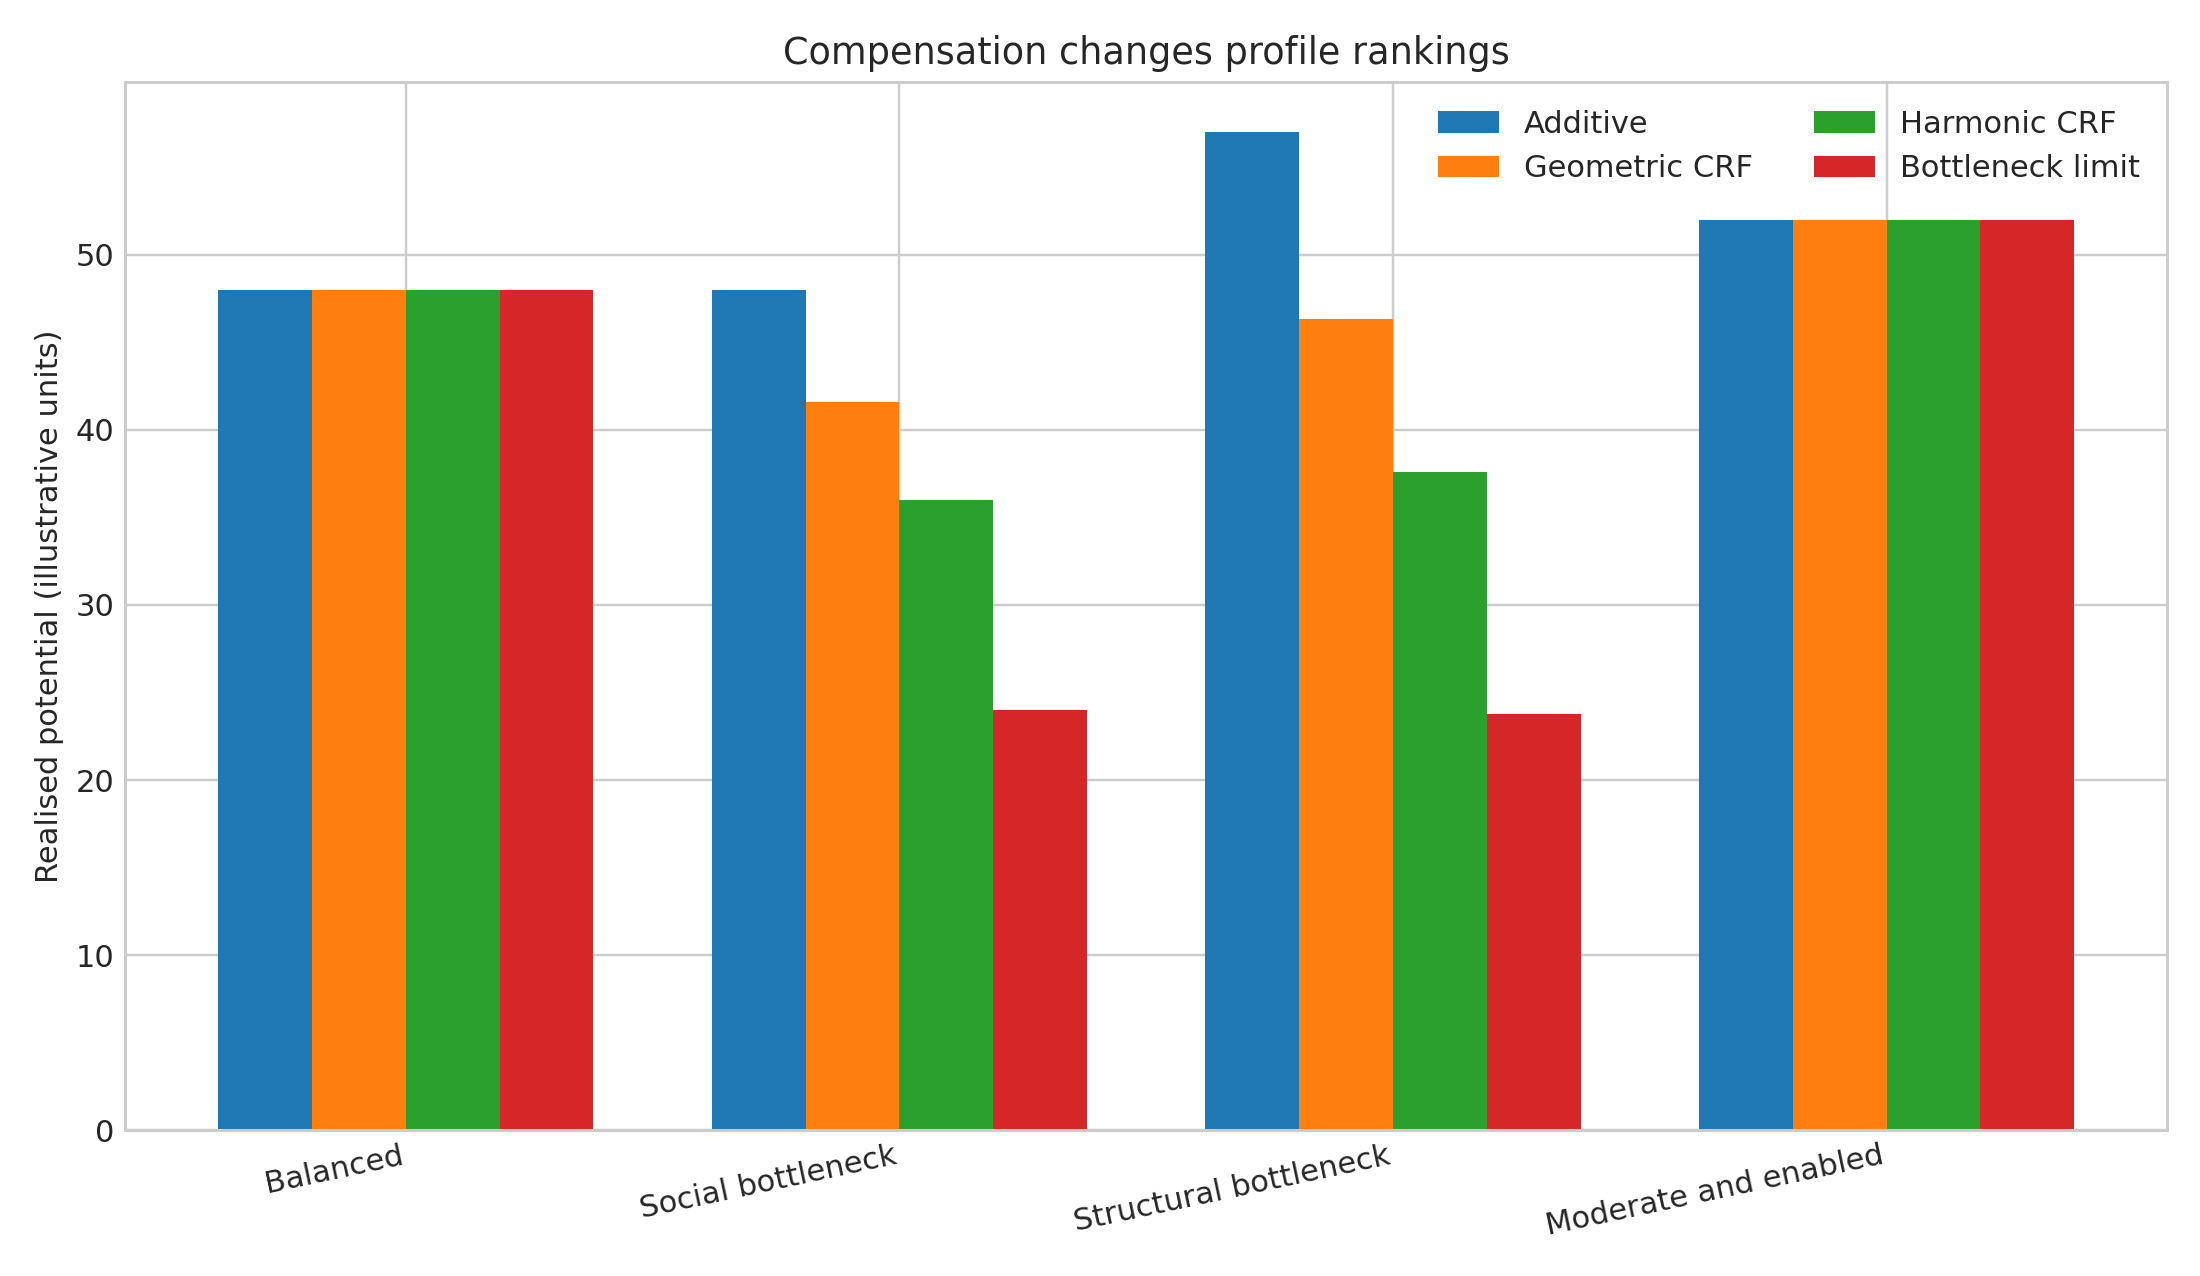
\includegraphics[width=0.9\textwidth]{Figures/crf_profile_comparison.png}
\caption{Illustrative profile rankings under compensatory and non-compensatory
aggregators. Profiles with equal average contextual resources can separate under
the CRF when one enabling domain is a bottleneck. Values are simulated.}
\label{fig:crf_profile_comparison}
\end{figure}

\begin{figure}[H]
\centering
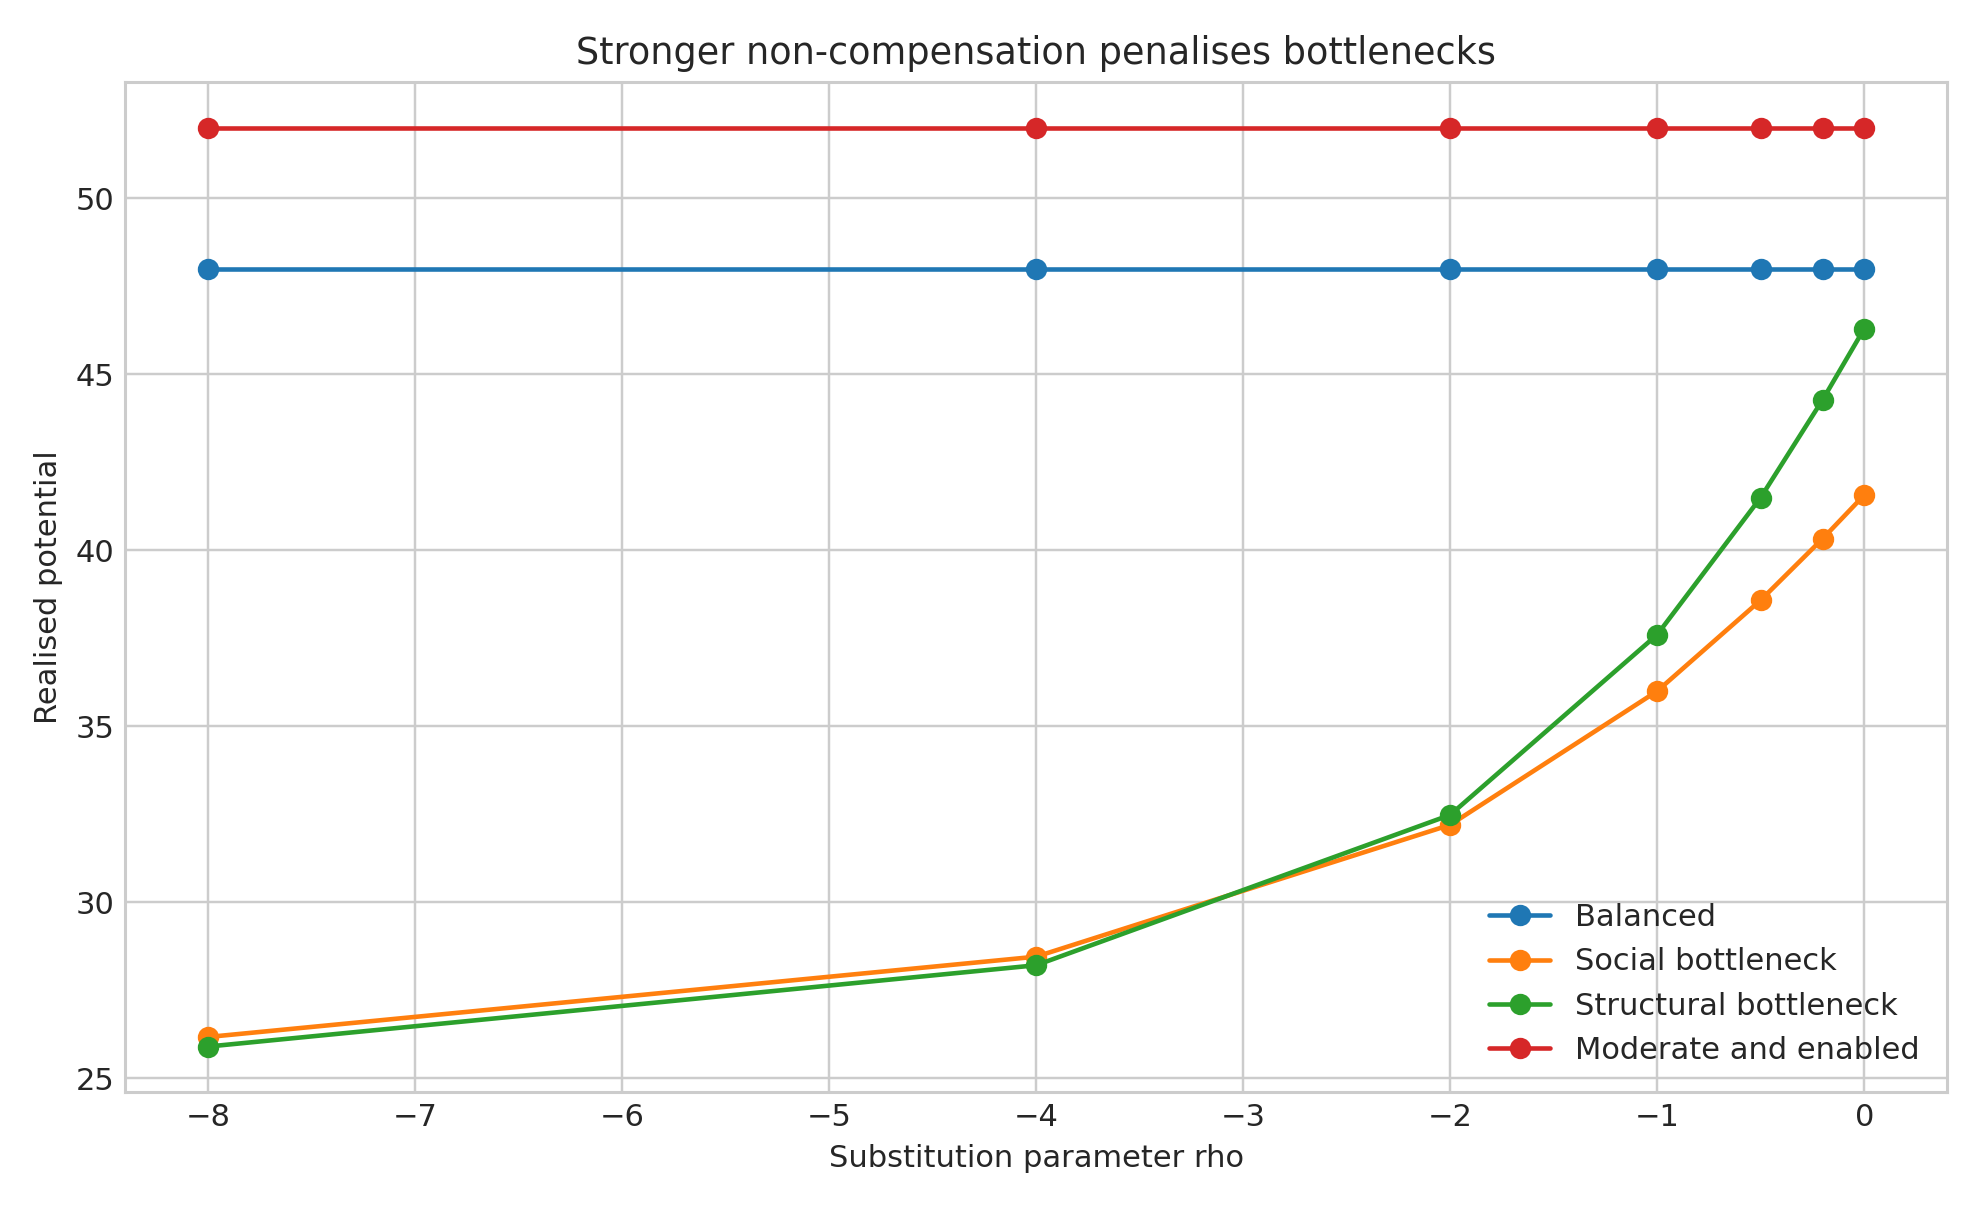
\includegraphics[width=0.9\textwidth]{Figures/crf_rho_sensitivity.png}
\caption{Sensitivity of realised potential to the substitution parameter $\rho$.
More negative values impose a stronger bottleneck penalty. Values are simulated.}
\label{fig:crf_rho_sensitivity}
\end{figure}

\begin{figure}[H]
\centering
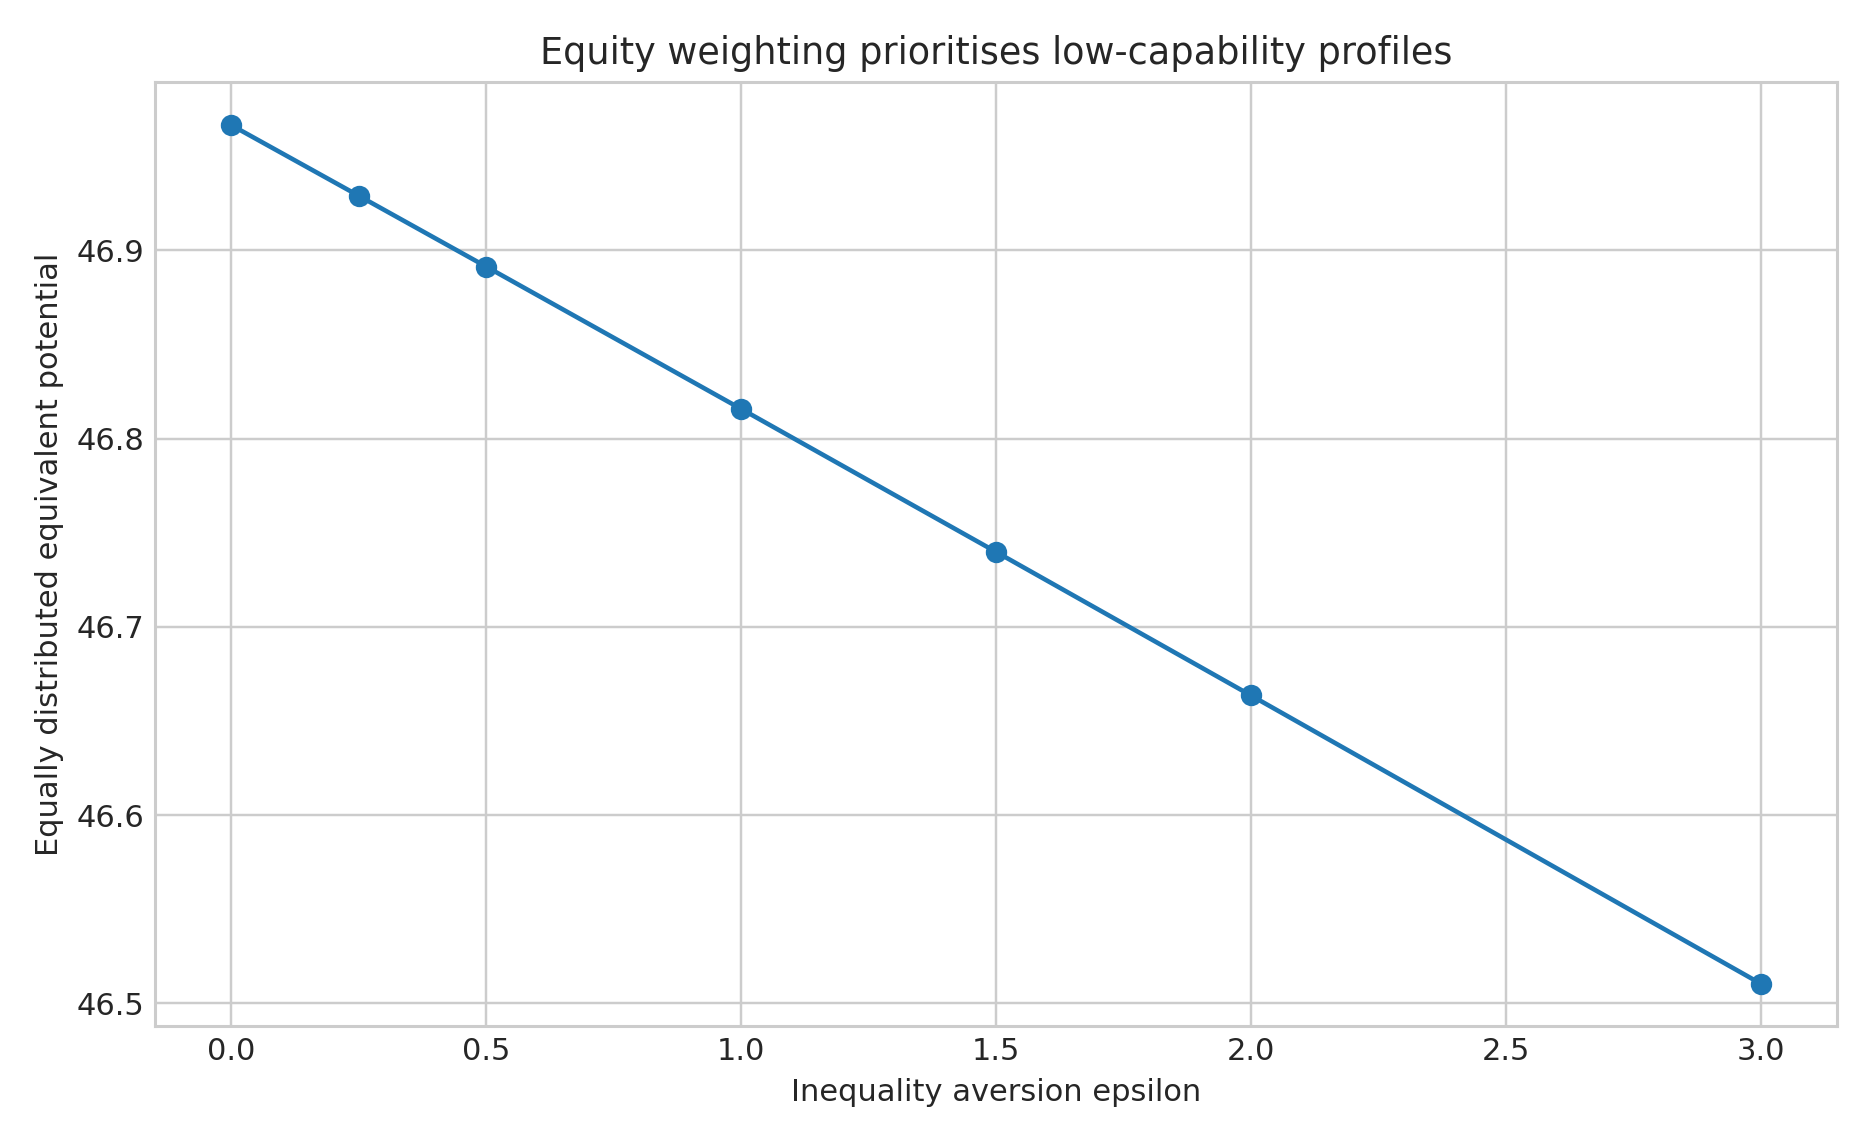
\includegraphics[width=0.9\textwidth]{Figures/crf_equity_aversion.png}
\caption{Equally distributed equivalent potential as inequality aversion
$\varepsilon$ increases. Declines indicate that low-capability profiles receive
greater normative weight. Values are simulated.}
\label{fig:crf_equity_aversion}
\end{figure}

The generated CSV files preserve every plotted value and include model-implied
marginal gains for biomedical, social, and burden-reducing interventions. These
gradients illustrate how aggregation can change priorities; they are not causal
treatment effects.

\section{Falsification and Empirical Comparison}
\label{sec:E-falsification}
The mathematical contribution is supported only if the following pre-specified
tests succeed:
\begin{enumerate}
 \item domain orientations and boundary behaviour are empirically plausible;
 \item CRF scores are stable under defensible normalisation choices;
 \item the non-compensatory model is compared with an additive composite, the SEM
 factor score, and less restrictive $\rho>0$ sensitivity models;
 \item paired bootstrap \citep{efron_tibshirani_1993,steyerberg_2019} estimates compare calibration, discrimination, and net
 benefit without tuning $\alpha$ or $\rho$ to the evaluation outcomes;
 \item subgroup analyses assess whether the model reduces or amplifies systematic
 error; and
 \item external validation evaluates transportability of both levels and gradients.
\end{enumerate}
Failure of these tests rejects or narrows the CRF; it does not invalidate the
separate latent measurement model.

\subsection{Head-to-head empirical protocol}
The empirical comparison uses the same analytic sample, imputations, resamples,
outcomes, and evaluation horizons for every representation:
\begin{enumerate}
 \item age-and-sex baseline;
 \item conventional comparator set (frailty, comorbidity, function, and QALY
 proxy);
 \item additive domain composite;
 \item primary SEM factor score;
 \item geometric CRF; and
 \item CRF sensitivity specifications for pre-declared $\rho$ values.
\end{enumerate}
All normalisation bounds, $\alpha$, $\rho$, and indicator directions are frozen
without reference to mortality or hospitalisation. Within each paired bootstrap
replicate the full measurement and prognostic pipeline is repeated. Reported
contrasts include calibration intercept and slope, time-specific Brier score \citep{brier_1950},
Harrell and Uno concordance \citep{uno_2011}, time-dependent AUC, and net benefit. Subgroup
calibration and error are reported across pre-specified equity strata.

\subsection{Success and rejection criteria}
The mathematical model is not declared useful merely because a CRF coefficient is
statistically significant. A strong mathematical--empirical contribution requires:
\begin{enumerate}
 \item rejection of the claim that the CRF is numerically redundant with the
 additive composite, demonstrated by meaningful profile or ranking differences;
 \item calibration and overall prediction error no worse than the additive and SEM
 alternatives, with paired uncertainty;
 \item either improved net benefit \citep{vickers_elkin_2006} over a clinically defensible threshold range or
 demonstrably clearer detection of structural bottlenecks;
 \item no material worsening of subgroup calibration or error; and
 \item qualitatively stable conclusions across reasonable normalisation bounds and
 pre-specified $\rho$ values.
\end{enumerate}
If these conditions fail, the central empirical claim for the CRF is narrowed to a
theoretical model, and the outcome-independent SEM score is retained as the
measurement backbone. If they hold internally but not externally, the claim is
restricted to the developmental population.

\subsection{Explicit rejection criteria}
The construct and its realisation model are rejected or narrowed if any pre-specified
condition holds under outcome-blind evaluation.
\begin{enumerate}\setlength{\itemsep}{2pt}
\item \textbf{Measurement collapse.} The three domains fail discriminant validity
($\mathrm{HTMT}>0.85$, or factor correlations above $0.90$), forcing a single factor.
\item \textbf{Determinacy failure.} The second-order factor-score determinacy \citep{grice_2001} falls
below $0.80$, so a person-level scalar cannot be reliably estimated.
\item \textbf{Prognostic non-inferiority deficit.} In optimism-corrected bootstrap
comparisons the full model fails to improve discrimination ($\Delta C\le 0$) or
prediction error over a parsimonious frailty or comorbidity index.
\item \textbf{Non-compensatory rejection.} The geometric CRF shows a worse calibration
slope, $|1-b_{\text{geom}}|>|1-b_{\text{add}}|$, or lower net benefit than an additive
composite.
\item \textbf{Invariance breakdown.} Scalar invariance \citep{putnick_bornstein_2016} fails across major groups and
partial invariance cannot restore fit, so group differences reflect measurement bias.
\end{enumerate}
If criterion~1 or~2 holds, the scalar metric is abandoned for the unaggregated
profile $(P,S,R)$. If criterion~4 holds, the non-compensatory hypothesis is refuted
and compensatory additive modelling is restored. Declaring these before the outcome
analysis is what makes the framework interrogable.

\section{Summary}
The CRF supplies the thesis with a dimensionally coherent and falsifiable
mathematical object. Its distinctive contribution is not the geometric mean alone,
but the combined axioms, non-compensatory interpretation, complementarity proof,
exact equity-gap decomposition, causal caveat, and pre-specified comparison with
the outcome-independent SEM metric.


\chapter{Results I: Development and Validation of the Measurement Model}

\label{ch:results1}

\begin{ataglance}[How to read this chapter]
The chapter asks one question and refuses to answer any other: can the three
domains be measured? Prediction is Chapter~\ref{ch:results2}'s problem, and
nothing here is allowed to consult it.

The order is the order in which a measurement claim can fail. Who is in the
sample (\S\ref{sec:sample}); whether the model can be estimated at all
(\S\ref{sec:anal-estimation}); whether the covariance structure the theory
implies matches the one observed (\S\ref{sec:anal-fit}); whether each indicator
belongs where the theory put it (\S\ref{sec:anal-loadings}); whether the
domains are reliable and, more demandingly, whether they are distinguishable
from one another (\S\ref{sec:anal-validity}); and only then whether the three
can legitimately be read as one thing (\S\ref{sec:anal-secondorder}). Scores
are derived last (\S\ref{sec:anal-scores}) and stress-tested
(\S\ref{sec:anal-robust}).

Two conventions run through the chapter. Every statistical term is given its
clinical counterpart at first use, so that a reader who thinks in diagnostic
tests can follow a reader who thinks in loadings. Where an example is needed,
it uses Profile~A of Table~\ref{tab:profiles}.
\end{ataglance}

This chapter presents the empirical evaluation of the proposed measurement model for the latent construct $H_{\text{potential}}$. The objective is to determine whether the theoretical framework developed in Chapter~\ref{ch:theory} can be operationalised as a statistically coherent higher-order latent variable within the National Health and Aging Trends Study (NHATS).

Unlike conventional frailty indices, which aggregate observable deficits into a summary score, the present model assumes that latent health potential is not directly observable but is reflected through several interconnected domains. The model therefore specifies three first-order latent constructs, Biomedical Potential, Social Modifiers, and Systemic Burdens, which together define the higher-order construct $H_{\text{potential}}$. The empirical task of this chapter is to evaluate whether the observed indicators reproduce the theoretical structure proposed earlier, and whether the resulting construct meets accepted standards of psychometric quality.

Following COSMIN recommendations for evaluating measurement instruments \citep{mokkink_2010, mokkink_2018}, the assessment proceeds in stages. The characteristics of the analytic sample are described first. The adequacy of the proposed factor structure is then evaluated by confirmatory factor analysis. Individual indicator performance is assessed through standardised factor loadings and explained variance. Internal consistency, convergent validity, and discriminant validity are examined next. Finally, the second-order structure is evaluated to determine whether the three domains can legitimately be interpreted as manifestations of a single higher-order construct.

The chapter concludes by deriving individual estimates of $H_{\text{potential}}$, which serve as the principal predictor in the prognostic analyses reported in Chapter~\ref{ch:results2}. The chapter therefore addresses the construct-validation component of Aim~2 and establishes whether the proposed representation has sufficient psychometric integrity for the predictive modelling that follows.

\begin{quote}
\small\itshape
Note to the reader. The numerical results in this chapter are produced by the analysis of NHATS described in Chapter~\ref{ch:methods}. Tables and figures are laid out for those results, and bracketed placeholders mark values to be inserted once the analysis is complete. This note is removed in the final version.
\end{quote}

\section{Analytic Sample}
\label{sec:sample}
The analytic sample was derived according to the inclusion and exclusion criteria set out in Chapter~\ref{ch:methods}. Participants were required to have sufficient information across the indicators of the three domains to permit latent-variable estimation. Observations with missingness above the pre-specified threshold were either excluded or handled by the multiple-imputation procedure described earlier, so that the estimation sample was neither reduced to complete cases alone nor biased by the ad hoc deletion of informative records.

Who is in the sample decides what the model can be asked. With that settled, the model itself has to be made to run, which in a three-factor structure is less automatic than it sounds.

The resulting sample comprises approximately 3\,500 community-dwelling adults aged 65 years and older at the Round~5 baseline. A sample of this size provides adequate power for a second-order structural equation model of the present complexity and exceeds conventional guidance for confirmatory factor analysis, which recommends several hundred observations depending on the number of indicators and the size of the loadings \citep{kline_2015, brown_2015}. A large sample also stabilises the estimation of standard errors and of the fit statistics reported below.

Table~\ref{tab:sample} summarises the demographic, clinical, and socioeconomic characteristics of the participants. These variables span biological health, functional status, and social circumstance, and they show substantial variation across the sample. This heterogeneity is the setting the analysis requires: it allows a test of whether a small number of latent domains can account for variation across a wide and apparently diverse set of indicators.

The observed characteristics are not treated as outcomes in their own right. Each is an empirical manifestation of one of the latent domains defined in the theoretical framework, and its distribution provides context for interpreting the measurement properties reported in the remainder of the chapter. Where a characteristic is markedly skewed or sparse in one tail, this is noted, because such features affect both the estimator chosen and the interpretation of the corresponding loading.

\begin{table}[h]
\centering
\caption{Baseline characteristics of the analytic sample (\hpval{N}{$N \approx 3\,500$}).}
\label{tab:sample}
\footnotesize
\renewcommand{\arraystretch}{1.2}
\begin{tabular}{p{6.5cm} p{4.5cm}}
\toprule
\textbf{Characteristic} & \textbf{Value} \\
\midrule
\hprows{sample}{%
Age, years, mean (SD) & [\,--\,] \\
Female, n (\%) & [\,--\,] \\
Multimorbidity, count of conditions, median (IQR) & [\,--\,] \\
Any ADL limitation, n (\%) & [\,--\,] \\
Any IADL limitation, n (\%) & [\,--\,] \\
Cognitive impairment, n (\%) & [\,--\,] \\
Positive depression screen (PHQ-2), n (\%) & [\,--\,] \\
Low social participation, n (\%) & [\,--\,] \\
Dual Medicare/Medicaid eligibility, n (\%) & [\,--\,] \\
Less than high-school education, n (\%) & [\,--\,] \\
Reported care delayed for cost or transport, n (\%) & [\,--\,] \\
}
\bottomrule
\end{tabular}
\end{table}

\medskip
\noindent\emph{[Placeholder: brief narrative on the composition of the sample, the balance of the domains, and any characteristic whose distribution bears on the estimation choices below.]}

\section{Estimation of the Measurement Model}
\label{sec:anal-estimation}
The measurement model was estimated by confirmatory factor analysis within the structural equation modelling framework of Chapter~\ref{ch:methods}. Three correlated first-order latent variables were specified, each measured by its own observed indicators, and together they define a single second-order latent factor representing $H_{\text{potential}}$. Fixing the pattern of loadings in advance, rather than letting the data determine which indicators belong to which factor, is what makes this a confirmatory test of the theory rather than an exploratory search.

Maximum likelihood estimation with robust standard errors served as the primary estimator, because it is efficient under approximately continuous measurement and tolerant of moderate departures from multivariate normality. Because several indicators are ordinal or categorical, the model was re-estimated with the weighted least squares mean- and variance-adjusted (WLSMV) estimator, which treats ordinal indicators through a threshold model rather than assuming interval measurement \citep{muthen_1984,rhemtulla_2012}, as implemented in \texttt{lavaan} \citep{rosseel_2012}. Agreement between the two estimators is not a formality: it provides evidence that the recovered structure reflects stable relationships in the data rather than an artefact of a single set of distributional assumptions. Where the two disagree, the WLSMV solution is given greater weight for the ordinal indicators, and the disagreement is reported.

Estimation was checked for convergence, admissibility, and local identification. Particular attention was paid to Heywood cases, negative residual variances, non-positive-definite covariance matrices, and standardised loadings at or above one, each of which can signal misspecification, empirical underidentification, or insufficient separation between constructs. Where a solution was inadmissible, the source was diagnosed before any change was made. Model respecification was considered only where a modification was supported at the same time by a substantive reading of the indicator and by the statistical evidence; changes driven by modification indices alone, without a theoretical rationale, were not made, since these capitalise on chance and inflate apparent fit.

\medskip
\noindent\emph{[Placeholder: convergence status, chosen estimator, treatment of ordinal indicators, admissibility of the solution, and any respecification with its justification.]}

\begin{reading}[Heywood cases and what they mean]
A Heywood case is a negative residual variance: the model says an indicator
contains less than none of its own noise, which is impossible. It is the
statistical equivalent of a laboratory returning a negative haematocrit. The
value is not merely surprising, it is outside the range the quantity can take,
and the correct response is to look for a fault in the machinery rather than to
report it.

Here the usual faults are two. Either the model has more parameters than the
data can support, so the estimate is unstable, which is empirical
underidentification. Or two domains are so highly correlated that the estimator
cannot tell them apart and drives a variance below zero to reconcile them. The
second diagnosis matters for the theory, because it would mean the three-domain
partition has failed in a way no amount of respecification can rescue.
\end{reading}

A model that converges to an admissible solution has cleared the lowest bar. Whether that solution reproduces what the data actually look like is the next question.

\section{Global Model Fit}
\label{sec:anal-fit}
The adequacy of the measurement structure was judged from several complementary fit indices rather than from any single statistic, because each index is sensitive to a different aspect of misfit. Interpretation rests on the overall pattern of evidence.

The comparative fit index (CFI) and the Tucker--Lewis index (TLI) measure improvement over an independence model in which the indicators are assumed uncorrelated. The root mean square error of approximation (RMSEA) measures residual misfit per degree of freedom, and so penalises unnecessary complexity; it is reported with its 90\% confidence interval, which conveys the precision of the estimate. The standardised root mean square residual (SRMR) is the average standardised difference between the observed and model-implied correlations, and gives a direct sense of how far the model reproduces the data. Together these indices assess whether the covariance structure implied by the theoretical model matches the covariance actually observed. Conventional thresholds are CFI and TLI of at least 0.95, RMSEA of at most 0.06, and SRMR of at most 0.08 \citep{hu_bentler_1999}.

The model chi-square is reported for completeness, but is not used as the primary criterion. In samples of several thousand, the chi-square test is sensitive to trivial departures from the model and will often be significant even when the model reproduces the data well. For this reason the approximate fit indices, which are less dependent on sample size, carry greater weight in the interpretation. Where all indices meet their thresholds, the latent structure is treated as an adequate representation of the observed relationships. Where one index falls short while the others hold, the shortfall is examined and interpreted rather than treated as an automatic rejection of the model.

\begin{table}[h]
\centering
\caption{Global fit of the second-order measurement model.}
\label{tab:fit}
\footnotesize
\renewcommand{\arraystretch}{1.2}
\begin{tabular}{p{4.5cm} p{3cm} p{3cm} p{2.2cm}}
\toprule
\textbf{Index} & \textbf{ML estimate} & \textbf{WLSMV estimate} & \textbf{Threshold} \\
\midrule
$\chi^2$ (df), $p$ & [\,--\,] & [\,--\,] & -- \\
CFI & [\,--\,] & [\,--\,] & $\geq 0.95$ \\
TLI & [\,--\,] & [\,--\,] & $\geq 0.95$ \\
RMSEA (90\% CI) & [\,--\,] & [\,--\,] & $\leq 0.06$ \\
SRMR & [\,--\,] & [\,--\,] & $\leq 0.08$ \\
\bottomrule
\end{tabular}
\end{table}

\medskip
\noindent\emph{[Placeholder: whether the model meets the fit criteria under each estimator, and interpretation of any index that does not.]}

\begin{reading}[Why the chi-square test is set aside]
The model chi-square tests a null hypothesis that the model reproduces the
population covariance matrix exactly. In a sample of several thousand it will
reject that null for departures too small to matter, which is the same
phenomenon a clinician meets when a trial of fifty thousand people finds a
statistically significant two-millimetre difference in blood pressure.

Significance answers whether a difference exists. It says nothing about whether
the difference is large enough to change anything. The approximate fit indices
are reported because they measure how far the model is from the data rather
than whether the distance is exactly zero.

The conventional cut-offs of 0.95 and 0.06 carry the opposite risk. They were
derived from simulations under specific conditions and have hardened into rules
that get applied everywhere, which is how an eGFR of 59 came to be treated as a
different kind of thing from an eGFR of 61. They are read here as reference
points and not as a pass mark.
\end{reading}

Global fit is an average over the whole model, and an average can hide a
single indicator sitting in the wrong domain. The loadings say where the fit
comes from.

\section{Measurement Quality: Factor Loadings}
\label{sec:anal-loadings}
Standardised factor loadings quantify the association between each observed indicator and its latent construct. A high loading indicates that the indicator captures a large share of the construct; a low loading indicates greater measurement error or that the indicator taps something beyond the intended construct. Loadings are read here not on statistical grounds alone but against the theoretical expectations set out in Chapter~\ref{ch:theory}.

Biomedical indicators are expected to show consistently strong positive relationships with Biomedical Potential, because multimorbidity, functional limitation, cognition, and psychological wellbeing directly reflect physiological and cognitive reserve. Social indicators are expected to show moderate to strong loadings on Social Modifiers, reflecting the broader environmental context that shapes health trajectories; some attenuation is anticipated here, since social participation and support are measured with more heterogeneity than clinical variables. Indicators of Systemic Burdens are expected to load together in a way that captures structural constraint operating independently of biological capacity, with the sign of each loading following the reverse-coding described in Chapter~\ref{ch:methods}.

The proportion of variance explained ($R^2$) for each indicator estimates its reliability within the model. Indicators with low explained variance are flagged: they may point to a domain that needs conceptual refinement, or to the need for additional observed measures in a later implementation of the construct. An indicator that loads weakly on its intended factor but appreciably on another is noted as a possible cross-loading, since this bears directly on the discriminant validity examined in the next section.

\begin{table}[h]
\centering
\caption{Standardised factor loadings by domain.}
\label{tab:loadings}
\footnotesize
\renewcommand{\arraystretch}{1.2}
\begin{tabular}{p{5.5cm} p{2.6cm} p{2.2cm} p{2cm}}
\toprule
\textbf{Indicator} & \textbf{Loading (SE)} & \textbf{$p$} & \textbf{$R^2$} \\
\midrule
\multicolumn{4}{l}{\textit{Biomedical Potential}} \\
\quad Multimorbidity & [\,--\,] & [\,--\,] & [\,--\,] \\
\quad ADL/IADL limitation & [\,--\,] & [\,--\,] & [\,--\,] \\
\quad Cognitive function & [\,--\,] & [\,--\,] & [\,--\,] \\
\quad Psychological wellbeing & [\,--\,] & [\,--\,] & [\,--\,] \\
\addlinespace
\multicolumn{4}{l}{\textit{Social Modifiers}} \\
\quad Social participation & [\,--\,] & [\,--\,] & [\,--\,] \\
\quad Support network & [\,--\,] & [\,--\,] & [\,--\,] \\
\quad Communication & [\,--\,] & [\,--\,] & [\,--\,] \\
\addlinespace
\multicolumn{4}{l}{\textit{Systemic Burdens}} \\
\quad Economic vulnerability & [\,--\,] & [\,--\,] & [\,--\,] \\
\quad Educational attainment & [\,--\,] & [\,--\,] & [\,--\,] \\
\quad Environmental stress & [\,--\,] & [\,--\,] & [\,--\,] \\
\quad Healthcare barriers & [\,--\,] & [\,--\,] & [\,--\,] \\
\bottomrule
\end{tabular}
\end{table}

\medskip
\noindent\emph{[Placeholder: which indicators load as expected, which are weak or cross-load, and what this implies for the domain definitions.]}

\begin{reading}[Reading a loading, and reading a cross-loading]
A standardised loading is the correlation between an indicator and the latent
variable it is meant to measure. Squared, it is the share of that indicator's
variance the construct explains, which is the model's estimate of how good a
window onto the construct the indicator is.

The clinical parallel is a diagnostic test's association with the disease it is
meant to detect. A loading of 0.8 is a test that tracks the underlying state
closely. A loading of 0.3 is a test that mostly measures something else.

A cross-loading is the more interesting failure. Suppose missed appointments
were entered as an indicator of Systemic Burdens, on the reasoning that they
record a transport barrier. If that indicator also loads on
Biomedical Potential, the model is saying that missed appointments partly track
how ill people are, which is true and which makes the indicator a poor measure
of structural constraint specifically. The remedy is conceptual rather than
statistical: find an indicator that records the barrier without recording the
illness.
\end{reading}

Strong loadings show that indicators track their own domain. They say nothing
about whether the three domains are three things or one thing wearing three
names, which is the question the validity evidence has to settle.

\section{Reliability and Construct Validity}
\label{sec:anal-validity}
Construct validation requires more than showing that indicators cluster together statistically. It requires evidence that they represent coherent theoretical domains and that those domains are empirically distinct from one another.

Reliability is assessed by composite reliability, which evaluates the internal consistency of each latent variable using the estimated loadings and so avoids the assumption of equal loadings that limits Cronbach's alpha \citep{raykov_1997}. Cronbach's alpha is also reported, to allow comparison with earlier literature that relies on it, but it is read as a lower bound rather than as the primary criterion. Values of composite reliability of about 0.70 or higher are taken to indicate adequate internal consistency for research use.

Convergent validity is assessed by the average variance extracted (AVE), the share of indicator variance a factor explains rather than leaves to measurement error. An AVE above 0.50 indicates that the factor accounts for more than half of the variance in its indicators, and so that the indicators converge on a common construct \citep{fornell_1981}. Where an AVE falls below this level while composite reliability remains adequate, this is noted, since it suggests a factor that is reliable but broad.

Discriminant validity addresses a different question: whether constructs that are theoretically distinct remain empirically separable. Two complementary criteria are used. The Fornell--Larcker criterion compares the square root of each factor's AVE with its correlations with the other factors; discriminant validity holds where the former exceeds the latter \citep{fornell_1981}. The heterotrait--monotrait ratio of correlations (HTMT) compares the average correlation of indicators across constructs with the average correlation within constructs, and is the more sensitive of the two in detecting a lack of separation \citep{henseler_2015}; values below about 0.85 support discriminant validity. Reporting both guards against the known limitations of either used alone. Table~\ref{tab:reliability} reports reliability and convergent validity, and Table~\ref{tab:discriminant} reports the discriminant-validity matrix.

\begin{definition}[Composite reliability]
\label{def:meas:omega}
Let a factor carry $k$ standardised indicators with loadings
$\lambda_1,\dots,\lambda_k$ and uncorrelated residuals of variance
$\theta_j=1-\lambda_j^{2}$. Composite reliability is
\begin{equation}
  \omega=\frac{\Bigl(\sum_{j=1}^{k}\lambda_j\Bigr)^{2}}
              {\Bigl(\sum_{j=1}^{k}\lambda_j\Bigr)^{2}+\sum_{j=1}^{k}\theta_j},
  \label{eq:omega}
\end{equation}
the share of the variance of the unit-weighted total score that the factor
explains \citep{raykov_1997}. Cronbach's $\alpha$ is the same quantity computed
as though every loading were the same size. Under that condition, called
tau-equivalence, $\alpha=\omega$; where the loadings differ, $\alpha\le\omega$,
and the gap widens with their spread. This is why $\alpha$ is read here as a
lower bound and $\omega$ as the estimate.
\end{definition}

\begin{definition}[Average variance extracted]
\label{def:meas:ave}
For the same factor,
\begin{equation}
  \mathrm{AVE}=\frac{1}{k}\sum_{j=1}^{k}\lambda_j^{2},
  \label{eq:ave}
\end{equation}
the mean share of an indicator's variance that the factor explains
\citep{fornell_1981}. An $\mathrm{AVE}$ above $0.50$ says the factor accounts
for more of the average indicator than measurement error does. It is an
average and not a total, so adding a further indicator of similar quality
raises $\omega$ and leaves $\mathrm{AVE}$ where it was. A factor can therefore
be reliable and still be broad.
\end{definition}

\begin{definition}[Fornell--Larcker criterion]
\label{def:meas:fl}
Let $\varphi_{kl}$ be the estimated correlation between factors $k$ and $l$.
Discriminant validity holds for factor $k$ by the Fornell--Larcker criterion
when
\begin{equation}
  \sqrt{\mathrm{AVE}_k}>\max_{l\neq k}\lvert\varphi_{kl}\rvert,
  \label{eq:fornell}
\end{equation}
that is, when the factor shares more variance with its own indicators than
with any other factor \citep{fornell_1981}.
\end{definition}

\begin{definition}[Heterotrait--monotrait ratio]
\label{def:meas:htmt}
Let factor $k$ have $p_k$ indicators and factor $l$ have $p_l$, and let
$r_{gh}$ denote an observed indicator correlation. The heterotrait--monotrait
ratio is the mean correlation between indicators of different factors divided
by the geometric mean of the two mean within-factor correlations:
\begin{equation}
  \mathrm{HTMT}_{kl}=
  \frac{\dfrac{1}{p_kp_l}\displaystyle\sum_{g=1}^{p_k}\sum_{h=1}^{p_l}r_{g^{(k)}h^{(l)}}}
       {\sqrt{\dfrac{2}{p_k(p_k-1)}\displaystyle\sum_{g<h}r_{g^{(k)}h^{(k)}}\;
              \cdot\;
              \dfrac{2}{p_l(p_l-1)}\displaystyle\sum_{g<h}r_{g^{(l)}h^{(l)}}}}.
  \label{eq:htmt}
\end{equation}
It estimates the correlation the two constructs would have if both were
measured without error, so a value near one says they are the same construct.
Values below about $0.85$ are taken to support discriminant validity
\citep{henseler_2015}.
\end{definition}

\begin{table}[h]
\centering
\caption{Reliability and convergent validity by domain.}
\label{tab:reliability}
\footnotesize
\renewcommand{\arraystretch}{1.2}
\begin{tabular}{p{4.5cm} p{2.6cm} p{2.6cm} p{2.6cm}}
\toprule
\textbf{Domain} & \textbf{Composite reliability} & \textbf{Cronbach's $\alpha$} & \textbf{AVE} \\
\midrule
Biomedical Potential & [\,--\,] & [\,--\,] & [\,--\,] \\
Social Modifiers & [\,--\,] & [\,--\,] & [\,--\,] \\
Systemic Burdens & [\,--\,] & [\,--\,] & [\,--\,] \\
\bottomrule
\end{tabular}
\end{table}

\begin{table}[h]
\centering
\caption{Discriminant validity: Fornell--Larcker (diagonal, $\sqrt{\text{AVE}}$; off-diagonal, factor correlations) with HTMT ratios in brackets.}
\label{tab:discriminant}
\footnotesize
\renewcommand{\arraystretch}{1.2}
\begin{tabular}{p{4.5cm} p{2.8cm} p{2.8cm} p{2.8cm}}
\toprule
\textbf{Domain} & \textbf{Biomedical} & \textbf{Social} & \textbf{Systemic} \\
\midrule
Biomedical Potential & [\,--\,] & [\,--\,] & [\,--\,] \\
Social Modifiers & [\,--\,] & [\,--\,] & [\,--\,] \\
Systemic Burdens & [\,--\,] & [\,--\,] & [\,--\,] \\
\bottomrule
\end{tabular}
\end{table}

\medskip
\noindent\emph{[Placeholder: reliability and validity interpretation, and whether the three domains are empirically distinguishable under both criteria.]}

\begin{reading}[Discriminant validity, and why it is the test this thesis can fail]
Discriminant validity asks whether two instruments are measuring the same thing
under different names. It is the psychometric form of a question clinicians ask
about new biomarkers: does this add anything to the panel we already run, or is
it troponin measured a second way?

The Fornell--Larcker criterion asks whether each domain shares more variance
with its own indicators than with the other domains. The heterotrait--monotrait
ratio compares correlations across constructs with correlations within them,
and it catches failures that Fornell--Larcker misses, which is why both are
reported.

The main risk here lies between Social Modifiers and Systemic Burdens. In
Profile~A both contextual domains are low. Weak social support and a barrier to
reaching care are conceptually different, one relational and one structural,
but they may not be empirically different, because the same disadvantage tends
to produce both. An HTMT ratio near 1.0 between those two domains would mean
the theory's three-way partition is a two-way partition in the data, and the
right response would be to report two domains rather than to insist on
three.
\end{reading}

\begin{workedexample}[meas-omega]{Composite reliability and AVE from a set of loadings}
Suppose the analysis returns standardised loadings of $0.82$, $0.74$, $0.68$
and $0.55$ for the four indicators of Biomedical Potential. The loadings sum
to $2.79$, so the squared sum is $7.784$. The residual variances are
$1-\lambda_j^{2}$ and sum to $2.015$. Equation~\eqref{eq:omega} gives
$\omega=7.784/(7.784+2.015)=0.794$.

Cronbach's $\alpha$ on the same model-implied covariance matrix is $0.789$.
The gap is small here because the loadings are not far apart; it would widen
if one indicator loaded at $0.30$ and another at $0.90$.

The squared loadings sum to $1.985$, so $\mathrm{AVE}=1.985/4=0.496$, a
fraction below the $0.50$ convention, and $\sqrt{\mathrm{AVE}}=0.704$. The
domain is reliable enough to use and explains slightly less than half of the
average indicator. That is a statement about the breadth of the indicator set
and not a reason to discard the domain.

\begin{wecode}[Python]
from hpv.measurement import (composite_reliability,
                             cronbach_alpha_from_loadings,
                             average_variance_extracted)

loadings = [0.82, 0.74, 0.68, 0.55]
print(f"omega {composite_reliability(loadings):.3f}")
print(f"alpha {cronbach_alpha_from_loadings(loadings):.3f}")
print(f"AVE   {average_variance_extracted(loadings):.3f}")
\end{wecode}

\weanswer{$\omega=0.794$, $\alpha=0.789$, $\mathrm{AVE}=0.496$. Asserted by
\texttt{test\_worked\_example\_reliability\_and\_ave\_from\_loadings} and
\texttt{test\_alpha\_equals\_omega\_only\_under\_equal\_loadings}.}
\end{workedexample}

\begin{workedexample}[meas-htmt]{An HTMT ratio, and where the 0.85 line falls}
Take the pair the chapter is most worried about, Social Modifiers against
Systemic Burdens. Suppose the three social indicators correlate at $0.52$,
$0.47$ and $0.44$ among themselves, mean $0.477$; the six pairs of systemic
indicators average $0.418$; and the twelve cross-construct correlations
average $0.294$.

Equation~\eqref{eq:htmt} gives
$0.294/\sqrt{0.477\times0.418}=0.659$. The two domains are
separable on this criterion, and not by a wide margin.

How far is the margin? Holding the within-construct correlations fixed, the
mean cross-construct correlation would have to rise from $0.294$ to $0.380$,
by about $29$ per cent, for the ratio to reach $0.85$. A single social
indicator that also records a structural barrier could move it that far, which
is the cross-loading problem of \S\ref{sec:anal-loadings} arriving at the
domain level.

\begin{wecode}[Python]
from hpv.measurement import htmt

within_social   = [0.52, 0.47, 0.44]
within_systemic = [0.49, 0.41, 0.38, 0.45, 0.36, 0.42]
cross = [0.34, 0.29, 0.31, 0.36,
         0.30, 0.26, 0.28, 0.33,
         0.27, 0.24, 0.25, 0.30]
print(f"HTMT {htmt(within_social, within_systemic, cross):.3f}")
print(f"at 0.85 the cross mean would be "
      f"{0.85 * (0.4767 * 0.4183) ** 0.5:.3f}")
\end{wecode}

\weanswer{$\mathrm{HTMT}=0.659$, against a threshold of $0.85$ that would need
a mean cross-construct correlation of $0.380$. Asserted by
\texttt{test\_definition\_and\_worked\_example\_htmt}.}
\end{workedexample}

If the domains are distinguishable, the framework's central claim can finally be
put: that these three distinguishable things are nevertheless facets of one
underlying quantity.

\section{Second-Order Structure and Domain Contributions}
\label{sec:anal-secondorder}
The defining claim of the framework is that Biomedical Potential, Social Modifiers, and Systemic Burdens are not free-standing latent variables but complementary dimensions of a single higher-order construct describing latent health potential. The second-order loadings provide the most direct test of that claim.

Strong and statistically significant second-order loadings indicate that the three domains share enough common variance to be read as manifestations of one overarching construct. Weak or non-significant loadings would indicate the opposite: that the domains are better treated as correlated but separate constructs, in which case the higher-order specification would not be supported and the interpretation of a single $H_{\text{potential}}$ would need to be revised. The direction of each second-order loading is examined against the theoretical expectation from Chapter~\ref{ch:theory}, namely that Biomedical Potential and Social Modifiers contribute positively and Systemic Burdens negatively, with the latter carried through the reverse-coding of its indicators.

The second-order loadings are interpreted as associations between the candidate general factor and the domain-level constructs, not as causal effects or policy weights. Their magnitude indicates how strongly each domain participates in the common covariance structure. Table~\ref{tab:secondorder} reports the estimated loadings and their uncertainty. If the higher-order model is not empirically supported, the domain profile is retained rather than forcing the domains into a scalar score.

\begin{table}[h]
\centering
\caption{Second-order loadings and standardised domain weights.}
\label{tab:secondorder}
\footnotesize
\renewcommand{\arraystretch}{1.2}
\begin{tabular}{p{4.5cm} p{2.8cm} p{3cm} p{2.4cm}}
\toprule
\textbf{Domain} & \textbf{$\hat{\gamma}_k$ (SE)} & \textbf{$\hat{\gamma}_k^{\text{std}}$} & \textbf{Weight $w_k$} \\
\midrule
Biomedical Potential & [\,--\,] & [\,--\,] & [\,--\,] \\
Social Modifiers & [\,--\,] & [\,--\,] & [\,--\,] \\
Systemic Burdens & [\,--\,] & [\,--\,] & [\,--\,] \\
\bottomrule
\end{tabular}
\end{table}

\medskip
\noindent\emph{[Placeholder: whether the second-order structure holds, whether the loading directions match the hypotheses of Chapter~\ref{ch:theory}, and how the domain weights are distributed.]}


\begin{proposition}[The higher-order layer with three domains is just identified]
\label{prop:meas:justid}
Standardise the three first-order factors of Definition~\ref{def:secondorder},
so their covariance matrix is the correlation matrix $\Phi$ with unit diagonal,
and write the higher-order layer as $\eta_k=\gamma_k\zeta+\delta_k$ with
$\operatorname{Var}(\zeta)=1$ and the $\delta_k$ mutually uncorrelated. The
layer has six free parameters, $\gamma_1,\gamma_2,\gamma_3$ and
$\psi_1,\psi_2,\psi_3$, and six moments to reproduce, the six distinct entries
of $\Phi$. Its degrees of freedom are zero. Whenever
$\gamma_1^{2}=\varphi_{12}\varphi_{13}/\varphi_{23}$ lies in $(0,1]$ and the
three correlations share a consistent sign pattern, the layer reproduces $\Phi$
exactly, the implied indicator covariance $\Sigma_Y$ equals that of the
correlated three-factor model, and $\chi^{2}$, CFI, TLI, RMSEA and SRMR take
identical values under the two models. Global fit therefore carries no
information about whether the higher-order structure holds.
\end{proposition}

\begin{proof}[Proof sketch]
Standardisation gives $\varphi_{kk}=\gamma_k^{2}+\psi_k=1$ and
$\varphi_{jk}=\gamma_j\gamma_k$ for $j\neq k$. The three off-diagonal
equations solve in closed form,
$\gamma_1=\sqrt{\varphi_{12}\varphi_{13}/\varphi_{23}}$,
$\gamma_2=\varphi_{12}/\gamma_1$, $\gamma_3=\varphi_{13}/\gamma_1$, and the
three diagonal equations then fix $\psi_k=1-\gamma_k^{2}$. Six equations, six
unknowns, no residual, so the fitted $\Phi$ equals the unrestricted $\Phi$ of
the correlated model and both models imply the same $\Sigma_Y$. The count is
the standard three-indicator identification result applied one level up
\citep{bollen_1989}. The only way the data can contradict the layer is
through admissibility: a solved $\gamma_k^{2}$ above one forces $\psi_k<0$,
which is a Heywood case at the second order.
\end{proof}

\begin{reading}[Why the fit table cannot settle the second-order question]
Table~\ref{tab:fit} reports the fit of the second-order model. Proposition
\ref{prop:meas:justid} says those numbers would be exactly the same if the
higher-order factor were deleted and the three domains simply allowed to
correlate. The second-order specification adds no constraint that the data can
refuse, so it cannot earn credit for fitting.

This is the psychometric version of a familiar clinical trap. A model with as
many parameters as observations will always pass through the observations, and
passing through them is then no evidence of anything. Fit indices are reported
in this chapter because they test the first-order structure, where there are
degrees of freedom to spend. They are silent one level up.

What is left to look at is the three estimated $\gamma_k$, their standard
errors, and whether the implied disturbance variances are positive. The next
box reads those quantities substantively.
\end{reading}

\begin{reading}[What a weak second-order loading would mean]
The second-order loadings decide whether $H_{\text{potential}}$ exists as a
single number or only as a profile. This is not a technicality that can be
settled by choosing the better-fitting model, because with only three
first-order factors the higher-order layer is close to just identified and good
fit is nearly guaranteed.

Suppose the loadings come back at 0.82 for Biomedical Potential, 0.78 for
Social Modifiers and 0.31 for Systemic Burdens. Global fit would probably still
look acceptable. The substantive reading would be that the general factor is
mostly a biological and social construct, and that structural burden is largely
doing its own work outside it.

Collapsing to a scalar in that situation would average away the one domain a
health system can act on directly. For Profile~A the scalar would rise with
$P$ and barely move with $R$, which defeats the practical purpose of the
measure. A weak third loading is therefore
a reason to report the profile, not a reason to report the scalar with a
caveat.
\end{reading}

If the higher-order structure holds, each participant can be given a number.
What that number is, and what it is not, needs stating before it is used.

\section{Derivation and Distribution of $H_{\text{potential}}$ Scores}
\label{sec:anal-scores}
Once the second-order model was estimated, individual factor scores were computed for each participant using Equation~\eqref{eq:factorscore}. Unlike a simple additive index, a factor score reflects both the measurement quality of the individual indicators and the estimated contribution of each domain, so that indicators measured with more error, or domains that contribute less to the common structure, carry proportionately less weight in a person's score.

The distribution of these scores describes latent health potential across the study population. Its shape is examined for ceiling and floor effects, for skewness, and for heterogeneity across participants, since each of these bears on how the score behaves as a predictor in the next chapter. A pronounced ceiling, for example, would compress differences among healthier participants and limit discrimination at that end of the range. Because the scores are standardised latent quantities rather than observed measurements, their absolute values carry no intrinsic clinical meaning. What is interpretable is relative position: a difference between two participants represents a difference in their estimated standing on the latent continuum defined by the measurement model. Figure~\ref{fig:score_dist} shows the distribution, and the accompanying text reports its mean, standard deviation, and range.

\begin{figure}[h]
\centering
\hpfig{score_dist}{\fbox{\parbox[c][4.5cm][c]{0.8\linewidth}{\centering \emph{[Figure placeholder: distribution of estimated $H_{\text{potential}}$ factor scores across the analytic sample.]}}}}
\captionsetup{justification=justified, width=\linewidth}
\caption{Distribution of estimated $H_{\text{potential}}$ scores in the analytic sample.}
\label{fig:score_dist}
\end{figure}

\medskip
\hptext{score_dist}{\noindent\emph{[Placeholder: descriptive statistics of the score, the shape of its distribution, and any feature that bears on its use as a predictor.]}}

These factor scores are the principal explanatory variable in the prognostic analyses of Chapter~\ref{ch:results2}, where their association with mortality and hospitalisation is formally evaluated.


\begin{definition}[Factor determinacy]
\label{def:meas:determinacy}
For a factor $\zeta$ with $\operatorname{Var}(\zeta)=1$, loading vector
$\lambda$ and indicator covariance $\Sigma_Y$, the determinacy of the score
$\widehat H$ of Definition~\ref{def:factorscore} is the correlation between the
factor and its own score,
\begin{equation}
  \rho_{\mathrm{det}}=\operatorname{corr}(\zeta,\widehat H)
  =\sqrt{\lambda^{\!\top}\Sigma_Y^{-1}\lambda}\,,
  \label{eq:determinacy}
\end{equation}
which lies in $[0,1]$ \citep{grice_2001}. Its square is the reliability of the
score. A determinacy of $0.90$ or above is the usual condition for treating
scores as a stand-in for the factor; below about $0.80$ two score sets built
from the same fitted model can rank people differently, and the score should
not be carried into a second analysis as though it were an observation.
\end{definition}

\begin{proposition}[Shrinkage of a factor score]
\label{prop:meas:shrinkage}
Take the one-factor case of Definition~\ref{def:factorscore} with
$\zeta\sim N(0,1)$, standardised indicators $y_j=\lambda_j\zeta+\varepsilon_j$
and independent $\varepsilon_j\sim N(0,\theta_j)$. Write
$I=\sum_j\lambda_j^{2}/\theta_j$ for the information the indicators carry about
$\zeta$. Then
\begin{equation}
  \widehat H=\mathbb E[\zeta\mid y]=\rho\,\widehat\zeta_{\mathrm{ML}},
  \qquad \rho=\frac{I}{1+I},
  \qquad \operatorname{Var}(\zeta\mid y)=1-\rho,
  \label{eq:shrinkage}
\end{equation}
where $\widehat\zeta_{\mathrm{ML}}=\bigl(\sum_j\lambda_jy_j/\theta_j\bigr)/I$.
Hence $\mathbb E[\widehat H\mid\zeta]=\rho\zeta$: the score is biased towards
the population mean, and the factor of compression is $\rho$, which is the
reliability of the score and the square of its determinacy
(Definition~\ref{def:meas:determinacy}).

In the linear normal case $I$ is the same for everyone. Two departures make it
person-specific. Where a participant leaves items blank, their $I$ is the sum
over the items they answered, so a sparse record compresses harder. Where the
indicators are ordinal and enter through the threshold model of
Chapter~\ref{ch:methods}, the posterior is a product of item likelihoods whose
peaks need not coincide; a discordant profile gives a flatter posterior, a
larger $\operatorname{Var}(\zeta\mid y)$ and so a smaller $\rho_i$. Compression
is worst for the participants whose indicators agree least with each other.

Chapter~\ref{ch:results2} inherits the consequence. A predictor compressed by
$\rho$ produces a coefficient attenuated by the same factor, which is
Proposition~\ref{prop:attenuation}.
\end{proposition}

\begin{proof}[Proof sketch]
The likelihood in $\zeta$ is Gaussian with precision $I$ centred at
$\widehat\zeta_{\mathrm{ML}}$; the prior is Gaussian with precision $1$ centred
at $0$. Conjugate updating adds precisions and takes the precision-weighted
mean, giving posterior precision $1+I$ and posterior mean
$I\widehat\zeta_{\mathrm{ML}}/(1+I)$. Since
$\mathbb E[\widehat\zeta_{\mathrm{ML}}\mid\zeta]=\zeta$, the compression
follows. That $\rho=\lambda^{\!\top}\Sigma_Y^{-1}\lambda$, and so equals the
squared determinacy of Definition~\ref{def:meas:determinacy}, is the
Sherman--Morrison identity applied to $\Sigma_Y=\lambda\lambda^{\!\top}+\Theta$.
The reading box below gives the clinical version.
\end{proof}

\begin{reading}[Shrinkage, or regression to the mean, in a factor score]
A factor score is a conditional expectation, so it is pulled towards the
population mean by an amount that depends on how much information the
indicators carry. Statisticians call this shrinkage; clinicians know the same
phenomenon as regression to the mean, which is why a single alarming blood
pressure reading is repeated before anyone acts on it.

The consequence is systematic rather than random. People whose indicators all
point the same way are estimated precisely and shrink little. People with an
unusual pattern are estimated imprecisely and shrink a lot. Profile~A,
moderate on the biomedical domain and low on both contextual domains, is the
second kind. Its point estimate will sit closer to the mean than its domain
values warrant, and its standard error will be wide.

This matters for the next chapter. Shrinkage compresses the range of the
predictor, and a compressed predictor produces a hazard ratio nearer to one
than the truth. The attenuation is not a nuisance to be apologised for; it is a
known direction of bias, and it means that a null result in
Chapter~\ref{ch:results2} is weaker evidence against the construct than a
positive result is for it.
\end{reading}

\begin{workedexample}[meas-shrink]{Shrinkage on a simulated latent variable}
Take the four Biomedical Potential loadings of Worked
Example~\ref{ex:meas-omega}. Their information is
$I=\sum\lambda_j^{2}/(1-\lambda_j^{2})=4.557$, so
$\rho=4.557/5.557=0.820$ and the determinacy is $\sqrt{0.820}=0.906$.

Simulate two hundred thousand people from the model, keep those whose true
$\zeta$ lies within $0.05$ of $-2.00$, and average their scores. The
proposition predicts $0.820\times(-2.00)=-1.64$, and the simulation returns
$-1.64$. A person two standard deviations below the mean is reported
as $1.64$ below it.

Now drop the two strongest indicators and score the same people on the
remaining two. Information falls to $1.294$ and $\rho$ to $0.564$, so the
proposition puts the same person at $0.564\times(-2.00)=-1.13$ and the
simulation returns $-1.15$, the difference being Monte Carlo noise over the
thousand or so people in the window. The true value has not changed. The
instrument has less to go on, so the model leans harder on the population
average.

\begin{wecode}[Python]
import numpy as np
from hpv.measurement import shrinkage_factor, factor_determinacy

lam = np.array([0.82, 0.74, 0.68, 0.55]); theta = 1 - lam**2
info = float(np.sum(lam**2 / theta))
rng = np.random.default_rng(20260902)
z = rng.standard_normal(200_000)
y = np.outer(z, lam) + rng.standard_normal((200_000, 4)) * np.sqrt(theta)
post = (y @ (lam / theta)) / (1 + info)
extreme = (z > -2.05) & (z < -1.95)
print(f"rho {shrinkage_factor(lam):.3f}  determinacy "
      f"{factor_determinacy(lam):.3f}")
print(f"true -2.00 comes back at {post[extreme].mean():.2f}")

lam2, theta2 = lam[2:], theta[2:]           # keep only the weaker two
info2 = float(np.sum(lam2**2 / theta2))
post2 = (y[:, 2:] @ (lam2 / theta2)) / (1 + info2)
print(f"on two indicators, rho {shrinkage_factor(lam2):.3f}, "
      f"-2.00 comes back at {post2[extreme].mean():.2f}")
\end{wecode}

\weanswer{A true score of $-2.00$ is reported as $-1.64$ at $\rho=0.820$, and
as $-1.15$ against a predicted $-1.13$ when only two indicators are observed.
Asserted by
\texttt{test\_worked\_example\_shrinkage\_on\_a\_simulated\_latent\_variable}
and \texttt{test\_proposition\_shrinkage\_compresses\_towards\_the\_mean}.}
\end{workedexample}

Everything above rests on a set of estimation choices that could have been made
differently. The last section puts them under strain.

\section{Robustness Checks}
\label{sec:anal-robust}
The stability of the measurement model was examined before its scores were carried forward. Three checks are reported. First, the model was re-estimated under the WLSMV estimator, and the loadings and fit compared with the maximum-likelihood solution, so that the recovered structure is not tied to one set of distributional assumptions. Second, the sensitivity of the solution to the indicator set was examined by re-estimating the model with individual indicators removed in turn, to confirm that no single indicator drives the structure. Third, where the sample size allows, measurement invariance \citep{meredith_1993,vandenberg_lance_2000} was tested across sex and across age band, by comparing configural, metric, and scalar models. Invariance matters because a score can only be compared across groups if the instrument measures the same construct in the same way in each group; a failure of invariance would qualify any later subgroup comparison and is reported as such.

\begin{definition}[The four levels of measurement invariance]
\label{def:meas:invariance}
Let groups $g=1,\dots,G$ each have loading matrix $\Lambda^{(g)}$, indicator
intercepts $\tau^{(g)}$ and residual covariance $\Theta^{(g)}$. Four nested
levels are tested in order \citep{meredith_1993,putnick_bornstein_2016}:
\begin{enumerate}
  \item \emph{Configural.} The same indicators load on the same factors in
        every group, with the same pattern of fixed and free entries in
        $\Lambda$. Nothing is constrained to be equal across groups.
  \item \emph{Metric, or weak.} Configural, with
        $\Lambda^{(1)}=\dots=\Lambda^{(G)}$. The unit of the latent scale is
        then common, so a regression coefficient on the factor may be
        compared across groups.
  \item \emph{Scalar, or strong.} Metric, with
        $\tau^{(1)}=\dots=\tau^{(G)}$. The origin of the scale is then common,
        so latent means may be compared.
  \item \emph{Strict.} Scalar, with
        $\Theta^{(1)}=\dots=\Theta^{(G)}$. Observed composite scores then carry
        the same measurement error in each group and may themselves be
        compared.
\end{enumerate}
Each level adds constraints to the one before, so the levels are compared by
change in approximate fit rather than by the difference in $\chi^{2}$ alone,
for the reason given in \S\ref{sec:anal-fit} \citep{vandenberg_lance_2000}.
\end{definition}

\medskip
\noindent\emph{[Placeholder: agreement between estimators, sensitivity to the indicator set, the level of measurement invariance achieved, and any limit this places on the generality of the construct.]}

\begin{reading}[Why invariance is not optional for this particular measure]
Measurement invariance asks whether the instrument means the same thing in
different groups. Configural invariance says the same indicators belong to the
same domains; metric invariance says they carry the same weight; scalar
invariance says that people with the same underlying level give the same
answers.

Only scalar invariance licenses comparing group means, and that is exactly what
a measure built to describe inequity is for. A score that reports lower
capability among poorer participants is worth nothing if the questions mean
something different to poorer participants. The failure would be invisible in
the results and would look like a finding.

The parallel is a symptom questionnaire that has not been validated in the
language it is being used in. It will still produce numbers, the numbers will
still differ between groups, and the difference will be an artefact of
translation. Where full invariance is not supported, the thesis reports the
non-invariance and narrows the comparison rather than proceeding as though the
question had not arisen.
\end{reading}

\section{Summary}
This chapter reported the development and validation of the $H_{\text{potential}}$ measurement model. Subject to the results above, it establishes whether the construct can be represented as a valid higher-order latent variable with acceptable fit, reliability, convergent validity, and discriminant validity, which is the first study hypothesis, and it derives the individual scores used in the analyses that follow. The next chapter tests whether those scores predict five-year all-cause mortality and first overnight hospital stay, and whether they add value over established measures.

\chapter{Prognostic Performance} \label{chap:dynamical_model}

\label{ch:results2}

\begin{ataglance}[How to read this chapter]
The question here is narrow. Chapter~\ref{ch:results1} asks whether the score can be measured. This chapter asks whether the number, once frozen, carries information about what happens to a person next, and whether it carries anything a frailty index, a comorbidity count, a record of what someone can do unaided or a health-utility proxy does not already say.

The sections are an order of tests, and each earns its place only if the one before it passed.

\textbf{Association first.} Until higher capability goes with a lower rate of death and of admission, nothing else is worth measuring. This is the weakest test the construct can face, and failing it ends the argument.

\textbf{Discrimination second.} An association can be real across a population and useless in front of one patient. Discrimination asks whether the score puts the people who go on to have the event above the people who do not. A wide average gap is compatible with heavy overlap between the two groups.

\textbf{Calibration third.} Ranking people correctly says nothing about whether the risk printed beside a name is the risk that person faces. Where a number crosses a threshold and triggers an action, the number has to be right in absolute terms and not merely in order.

\textbf{Only then the comparison.} A measure that passes all three can still be redundant. The comparison against frailty, comorbidity, functional status and a health-utility proxy, and the incremental test that follows it, is the test the construct is most likely to fail. It is placed last because it is only interesting once the construct has been shown to work on its own.

Two further sections guard the results instead of extending them. A combined endpoint checks that the co-primary findings do not depend on how the outcome was cut, and the treatment of missing data and of optimism asks how much of the performance above would survive contact with new patients drawn from the same population.

Mrs~A is used throughout to keep the arithmetic honest. Every worked number below is conditional on a result the analysis has not yet returned, and the placeholders are left empty on purpose.
\end{ataglance}

\begin{quote}
\small\itshape
Note to the reader. The numerical results in this chapter are produced by the analysis of the National Health and Aging Trends Study described in Chapter~\ref{ch:methods}. Tables and figures below are laid out for those results; bracketed placeholders mark values to be inserted once the analysis is complete. Figure and derivation blocks are reserved in place and marked accordingly. This note is removed in the final version.
\end{quote}

\noindent The preceding chapter established the psychometric properties of the proposed $H_{\text{potential}}$ construct and demonstrated that it can be estimated reliably as a multidimensional latent variable representing an individual's underlying capacity for health. Confirmatory factor analysis supported the theoretical measurement model, evidence of construct validity was obtained through the relationships among the latent domains, and the resulting factor scores provided a quantitative representation of each participant's estimated health potential. These findings addressed the first component of the study by demonstrating that the construct is measurable and internally coherent. However, establishing a valid measurement model represents only one stage in the development of a clinically meaningful health metric. A construct intended to inform healthcare decision-making must also demonstrate that it predicts future outcomes of practical clinical importance.

This chapter therefore shifts from measurement to prediction. Whereas Chapter~\ref{ch:results1} examined whether the proposed latent construct could be estimated consistently from observed indicators, the present chapter evaluates whether those estimates possess prognostic value. Prognostic validity concerns the extent to which variation in the latent score corresponds to subsequent differences in health outcomes. If the theoretical framework underpinning the $H_{\text{potential}}$ is correct, individuals with higher values of the latent construct should exhibit greater resilience, maintain functional independence for longer periods, and experience fewer adverse health events during follow-up. Conversely, lower scores should identify individuals at increased risk of clinical deterioration, unplanned healthcare utilisation and mortality. Demonstrating such relationships is essential if the construct is to progress beyond a theoretical model towards a practical tool capable of supporting risk stratification and personalised clinical management. Using the individual factor scores derived in Chapter~\ref{ch:results1}, this chapter tests, as confirmatory evidence, the association of the $H_{\text{potential}}$ with each of two pre-specified prognostic endpoints, quantifies its discrimination and calibration, compares it against established measures, and assesses its incremental value and clinical utility, following the prognostic plan of Section~\ref{sec:prognostic} and the performance and benchmarking plan of Section~\ref{sec:performance}. Construct validity, reported in Chapter~\ref{ch:results1}, is the study's primary outcome; the analyses here are confirmatory. All prognostic analyses, association, discrimination, calibration, comparison, and clinical utility, are carried out for each co-primary endpoint separately, with multiplicity handled according to the pre-specified inferential plan. This addresses Aim~3.

Within contemporary prognostic research, the evaluation of prediction models extends substantially beyond demonstrating statistical significance. A model may exhibit a highly significant association with an outcome while remaining of limited clinical value if it fails to distinguish accurately between individuals who do and do not experience the event of interest, produces poorly calibrated risk estimates, or provides no improvement over simpler existing approaches. Consequently, international guidance on prognostic model evaluation emphasises that multiple dimensions of model performance must be considered simultaneously, including association, discrimination, calibration, internal validity and clinical usefulness \citep{steyerberg_2019,vancalster_2019,collins_2015}. Together these criteria say more about predictive performance than hypothesis testing alone, and they form the analytical framework adopted throughout this chapter.

The conceptual distinction between explanatory modelling and prognostic modelling is particularly important in the context of this research. Explanatory analyses seek to understand causal mechanisms and quantify the independent contribution of specific variables to observed outcomes. Prognostic analyses, by contrast, seek to estimate the probability that a future event will occur for an individual given their current characteristics, irrespective of whether every predictor has a direct causal interpretation. Although the present study is grounded in a substantive theoretical model of health potential, its immediate objective is prognostic rather than causal. The primary question is therefore not whether each component of the latent construct causes improved health outcomes in isolation, but whether the integrated construct captures clinically meaningful information that predicts future health trajectories more accurately than existing approaches. This distinction underlies the choice of statistical methods and the interpretation of the results presented in the following sections.

The proposed $H_{\text{potential}}$ differs fundamentally from conventional health metrics in that it represents an estimate of latent capacity rather than current disease burden or existing disability. Traditional prognostic indices, such as comorbidity counts or frailty measures, primarily quantify accumulated deficits that are already clinically apparent. Although these measures have demonstrated prognostic utility across numerous populations, they are generally designed to describe deterioration that has already occurred. In contrast, the conceptual framework developed in this thesis proposes that health should be understood as a dynamic latent capacity that exists prior to observable clinical decline. From this perspective, adverse outcomes such as hospitalisation and mortality represent downstream manifestations of declining health potential rather than the construct itself. If this theoretical distinction is valid, the $H_{\text{potential}}$ should provide prognostic information that complements existing measures of disease burden and functional impairment instead of duplicating them.

This distinction has important implications for preventative healthcare. Identifying individuals only after substantial functional decline has occurred necessarily limits the opportunity for intervention. Conversely, a measure that captures latent health capacity before overt deterioration becomes clinically manifest may enable earlier identification of vulnerable individuals and support interventions while greater physiological reserve remains. Such an approach aligns with contemporary models of healthy ageing and preventative medicine, which increasingly emphasise maintaining intrinsic capacity \citep{who_2015_ageing,cesari_2018} rather than simply treating disease after its onset. Consequently, demonstrating the prognostic performance of the $H_{\text{potential}}$ has implications extending beyond statistical model development to broader questions regarding the measurement and management of health across the life course.

To evaluate these propositions, the analyses reported in this chapter employ prospective survival modelling using data from the National Health and Aging Trends Study (NHATS). The NHATS provides a uniquely suitable platform for this evaluation because it combines detailed multidimensional assessments of health status with longitudinal follow-up for clinically important outcomes. Repeated outcome ascertainment, detailed demographic and clinical information and nationally representative sampling together allow the proposed construct to be evaluated within a real-world ageing population rather than under highly selected experimental conditions. The prospective design also ensures that predictor measurements precede outcome occurrence, thereby supporting valid prognostic inference.

The endpoints considered throughout this chapter are two co-primary outcomes, analysed separately: all-cause mortality and first unplanned hospitalisation, each within five years of baseline assessment. The two are analysed separately because death is an absorbing, terminal event while unplanned hospitalisation is a recurrent, non-fatal event, and they are driven by different clinical and social processes. Combining them in one endpoint would obscure these differences, so each is fitted in its own survival model and family-wise error across the two co-primary tests is controlled. A combined time-to-first-event endpoint, mortality or unplanned hospitalisation whichever comes first, is analysed later in the chapter only as a sensitivity check on the co-primary results; it is not a primary endpoint.

Consistent with the statistical analysis plan outlined in Chapter~\ref{ch:methods}, prognostic performance is evaluated across several complementary dimensions. First, the association between the $H_{\text{potential}}$ and each co-primary endpoint is examined using Cox proportional hazards \citep{cox_1972} regression, before and after adjustment for basic demographic characteristics. Second, the discriminative ability of the resulting model is evaluated using Harrell's concordance statistic and Uno's inverse-probability-of-censoring weighted concordance statistic, and its calibration through calibration-in-the-large, the calibration slope and graphical assessment. Third, the performance of the $H_{\text{potential}}$ is compared directly with established measures currently used to characterise health status in ageing populations. Fourth, the incremental value of the construct is evaluated by examining changes in predictive performance when it is added to conventional prognostic models, and its clinical utility through decision-curve analysis. Finally, recognising that prediction models developed within a single dataset are susceptible to optimism arising from overfitting, the stability of the estimated performance is assessed through multiple imputation for missing data and bootstrap internal validation.

Throughout this chapter, effect estimates are presented together with 95\% confidence intervals in accordance with current recommendations for the reporting of prognostic studies. Where appropriate, statistical significance is reported using two-sided hypothesis tests with an $\alpha$ level of 0.05. However, interpretation is based primarily upon the magnitude, precision and clinical relevance of the estimated effects rather than statistical significance alone. The analyses presented here therefore address the third aim of the study by determining whether the $H_{\text{potential}}$ functions as a meaningful predictor of future health outcomes, and form the empirical bridge between the theoretical development of the construct and its subsequent application to disease-specific populations examined in the following chapter.

% =====================================================================
\section{Outcomes and Follow-up}
\label{sec:prog-outcomes}
% =====================================================================

\noindent Every quantity in this chapter is a rate, and a rate needs a denominator of time actually spent at risk. Two decisions fix that denominator: when a person stops contributing time, and whether the reason they stopped is one the model may ignore. Getting either wrong moves every estimate that follows.

\noindent Over five years of follow-up, the two co-primary outcomes are time to all-cause mortality and time to first unplanned hospitalisation, each analysed separately. Table~\ref{tab:events} reports the number of events, person-years of follow-up, and censoring for each endpoint. Figure~\ref{fig:km_overall} shows the cumulative incidence of each co-primary endpoint across the follow-up period.

\begin{table}[htbp]
\centering
\caption{Events and follow-up over five years.}
\label{tab:events}
\footnotesize
\renewcommand{\arraystretch}{1.2}
\begin{tabular}{p{7cm} p{4cm}}
\toprule
\textbf{Quantity} & \textbf{Value} \\
\midrule
All-cause deaths, n (\%) & [\,--\,] \\
First unplanned hospitalisations, n (\%) & [\,--\,] \\
Combined endpoint (sensitivity), n (\%) & [\,--\,] \\
Median follow-up, years (IQR) & [\,--\,] \\
Total person-years & [\,--\,] \\
Censored before event, n (\%) & [\,--\,] \\
\bottomrule
\end{tabular}
\end{table}

\begin{figure}[htbp]
\centering
\fbox{\parbox[c][5cm][c]{0.8\linewidth}{\centering \emph{[Figure placeholder: Kaplan--Meier \citep{kaplan_meier_1958} / cumulative-incidence curves for each co-primary endpoint over five years, with numbers at risk.]}}}
\captionsetup{justification=justified, width=\linewidth}
\caption{Cumulative incidence of each co-primary endpoint, all-cause mortality and first unplanned hospitalisation, over five years of follow-up.}
\label{fig:km_overall}
\end{figure}

A few terms in Table~\ref{tab:events} carry more weight than their brevity suggests. Censoring, a patient who is alive at last contact and whose later fate is unknown, is not a missing outcome. It is a known stretch of event-free time followed by silence, and the models below use the time and throw nothing away. A competing risk, an event that removes the patient from being at risk of the one you care about, is a different animal: for first unplanned hospitalisation, a death at home settles the question, because the admission can no longer occur. Immortal time, a period in which the outcome could not by construction have occurred, is avoided here by starting the clock at the baseline interview for everyone, so that nobody accrues follow-up during an interval in which they were event-free by definition.

\begin{reading}[Death before admission is not censoring]
Censoring means the fate is unknown: the person was alive and unadmitted when last seen, and might have been admitted the following week. Death before admission is not that. The admission will never happen. Treating the death as censoring instructs the estimator to assume the person who died would have gone on to be admitted at the same rate as those still alive, which is the one thing that cannot be true.

The size of the error is easy to see with constant rates. Take a group in which unplanned admissions occur at $0.15$ per person-year and deaths at $0.10$ per person-year. Over five years the chance of leaving the event-free state at all is $1-\exp\{-(0.15+0.10)\times5\}=1-\exp(-1.25)=0.71$, and admissions account for $0.15/0.25=60$ per cent of those exits, so the cumulative incidence of admission is $0.60\times0.71=0.43$. Treat the deaths as censoring and the Kaplan--Meier complement returns $1-\exp(-0.15\times5)=1-\exp(-0.75)=0.53$, ten percentage points too high.

Now take the group the measure exists to find. Hold the admission rate at $0.15$ and raise the death rate to $0.25$. True cumulative incidence of admission falls to $(0.15/0.40)\times\{1-\exp(-2)\}=0.375\times0.865=0.32$, because so many die first, while the censoring-based figure is unchanged at $0.53$. The overstatement has grown from ten points to twenty-one. The error is worst exactly where the frailest patients are, so a measure built for them would be judged on inflated numbers. This is why the analysis for admission uses a cause-specific hazard \citep{prentice_1978} and reports cumulative incidence, with a subdistribution model \citep{fine_gray_1999} as a check.
\end{reading}

With the events counted and the clock defined for each endpoint, the weakest test can be run: whether events arrive at a different rate for people with different scores.

% =====================================================================
\section{Association of the $H_{\text{potential}}$ with the Co-Primary Outcomes}
\label{sec:assoc}
% =====================================================================

\noindent A score can be measured well and still carry no news about the future. The test that decides whether the rest of the chapter is worth reporting is whether people with more of the construct have their events later, or not at all, than people with less of it.

\noindent The primary objective of this stage of the analysis was to determine whether the proposed $H_{\text{potential}}$ provides independent prognostic information regarding future adverse health outcomes. Whereas the previous chapter established that the latent construct can be measured reliably, the present analysis examines whether variation in that construct is associated with the subsequent occurrence of clinically meaningful events. Demonstrating such an association is a necessary prerequisite for establishing the prognostic validity of the proposed framework. If the theoretical model is correct, participants with higher levels of health potential should experience a lower risk of mortality or unplanned hospitalisation during follow-up than those with lower scores.

The relationship between the $H_{\text{potential}}$ and each co-primary endpoint was evaluated using Cox proportional-hazards regression, as specified in the statistical analysis plan and in Equation~\eqref{eq:cox}. Mortality and first unplanned hospitalisation are each fitted in a separate model, and family-wise error across the two co-primary tests is controlled. The Cox model was selected because it provides a semi-parametric framework for analysing time-to-event data without requiring specification of the underlying baseline hazard function \citep{cox_1972}. This flexibility makes the model particularly appropriate for longitudinal cohort studies in which participants contribute different lengths of follow-up and where right censoring is present due to loss to follow-up or administrative study completion. Rather than modelling the probability of an event at a fixed point in time, the Cox model estimates the instantaneous hazard of experiencing the event, allowing both the timing and occurrence of adverse outcomes to contribute to the analysis.

Individual participant scores for the $H_{\text{potential}}$ were obtained from the latent measurement model described in Chapter~\ref{ch:results1}. To improve interpretability and facilitate comparison with existing prognostic studies, the latent scores were standardised before entry into the survival models. Consequently, hazard ratios are reported per one standard deviation increase in the $H_{\text{potential}}$. Expressing effects in standard deviation units avoids dependence upon the arbitrary scale of the latent variable and permits direct comparison with effect sizes reported for other prognostic indices. A hazard ratio below one therefore indicates that higher health potential is associated with a reduced instantaneous risk of experiencing the endpoint, whereas a hazard ratio above one would indicate an increased risk.

Two regression models were estimated. The first was an unadjusted model containing only the $H_{\text{potential}}$, quantifying the overall association between the latent construct and subsequent health outcomes. The second model adjusted for age and sex, which were selected a priori because both variables are among the strongest and most consistently replicated predictors of mortality, hospitalisation and functional decline in older adults. Age exerts a pervasive influence on virtually every dimension of health, including physiological reserve, functional capacity, chronic disease burden and mortality risk, and important sex differences exist in survival, multimorbidity, disability trajectories and healthcare utilisation. Demonstrating that the association persists after adjustment would provide evidence that the construct captures additional prognostic information not explained solely by age or biological sex. The regression coefficients estimated by the Cox model were exponentiated to produce hazard ratios together with corresponding 95\% confidence intervals. Table~\ref{tab:hr} presents the estimated hazard ratios for the unadjusted and age- and sex-adjusted models, for each co-primary endpoint.

\begin{table}[htbp]
\centering
\caption{Association of the $H_{\text{potential}}$ with each co-primary outcome (hazard ratio per one standard deviation increase in the latent score).}
\label{tab:hr}
\footnotesize
\renewcommand{\arraystretch}{1.2}
\begin{tabular}{p{6cm} p{3.2cm} p{2.2cm}}
\toprule
\textbf{Endpoint and model} & \textbf{HR (95\% CI)} & \textbf{$p$} \\
\midrule
\multicolumn{3}{l}{\textit{All-cause mortality}} \\
\quad Unadjusted & [\,--\,] & [\,--\,] \\
\quad Adjusted for age and sex & [\,--\,] & [\,--\,] \\
\addlinespace
\multicolumn{3}{l}{\textit{First unplanned hospitalisation}} \\
\quad Unadjusted & [\,--\,] & [\,--\,] \\
\quad Adjusted for age and sex & [\,--\,] & [\,--\,] \\
\bottomrule
\end{tabular}
\end{table}

The estimand and the partial-likelihood machinery underlying these estimates are set out below for completeness.

\begin{derivation}[Cox partial likelihood for the $H_{\text{potential}}$ hazard ratio]
\label{der:cox}
For $Z_i=H_{i,\mathrm{std}}$, let
$h_i(t)=h_0(t)\exp(\beta Z_i+\boldsymbol\gamma^{\mathsf T}\mathbf c_i)$.
Ignoring ties for exposition, the partial likelihood is
\[
 L_p(\boldsymbol\theta)=\prod_{i:\delta_i=1}
 \frac{\exp(\boldsymbol\theta^{\mathsf T}\mathbf v_i)}
 {\sum_{j\in R(t_i)}\exp(\boldsymbol\theta^{\mathsf T}\mathbf v_j)},
\]
where $\mathbf v_i=(Z_i,\mathbf c_i^{\mathsf T})^{\mathsf T}$ and right-censored
participants contribute through risk sets until censoring. Differentiating
$\log L_p$ gives the observed-minus-risk-set-expected covariate score; the
negative Hessian is the observed information. Thus $\exp(\widehat\beta)$ is the
hazard ratio per one-SD higher score. Efron's approximation is used for tied
event times and robust uncertainty is considered when survey clustering applies.
\end{derivation}

\begin{definition}[Hazard function and hazard ratio]
\label{def:prog2:hazard}
For a survival time $T$ with survivor function $S(t)=\Pr(T>t)$ and density
$f$, the hazard function is
\begin{equation}
  h(t)=\lim_{\Delta\downarrow0}\frac{1}{\Delta}
       \Pr\{t\le T<t+\Delta\mid T\ge t\}
      =\frac{f(t)}{S(t)}
      =-\frac{\mathrm{d}}{\mathrm{d}t}\log S(t),
  \label{eq:hazard}
\end{equation}
the rate at which the event arrives among those it has not yet reached. It
has units of one over time and is not bounded above by one, so it is not a
probability. Integrating gives the cumulative hazard
$H(t)=\int_0^t h(u)\,\mathrm{d}u$ and $S(t)=\exp\{-H(t)\}$.

The hazard ratio between two people is $h_i(t)/h_j(t)$. Under the Cox model
of Definition~\ref{def:cox} it equals
$\exp\{\beta_H(H_i-H_j)+\boldsymbol\gamma^{\mathsf T}(\mathbf x_i-\mathbf x_j)\}$,
which does not depend on $t$; that constancy is the proportional-hazards
assumption tested in \S\ref{sec:prog-ph}. A hazard ratio is a multiplier on a
rate. It becomes a difference in risk only once a baseline cumulative hazard
is supplied, by way of $S(t)=\exp\{-H(t)\}$.
\end{definition}

Interpretation of the hazard ratio follows conventional principles of survival analysis. A hazard ratio of 1.00 would indicate no association between the $H_{\text{potential}}$ and the outcome. Values below one imply that higher levels of health potential are associated with a lower hazard of experiencing death or hospitalisation during follow-up. For example, an estimated hazard ratio of 0.80 would correspond to an approximately 20\% reduction in the instantaneous risk of the endpoint per standard deviation increase in the latent score. Interpretation focuses primarily on the magnitude of the estimated hazard ratio, the width of the associated confidence interval, and the consistency of findings across the adjusted and unadjusted models. If the hazard ratio changes only minimally following adjustment for age and sex, this would suggest that the $H_{\text{potential}}$ captures information beyond basic demographic risk factors; substantial attenuation towards the null would instead indicate that much of the observed association is explained by demographic differences.

\begin{reading}[What a hazard ratio is, and what it is not]
A hazard ratio is a multiplier on instantaneous risk. It says how much faster events arrive for one person than another at any given moment, among those still event-free at that moment. It is not a ratio of five-year risks, it is not a probability, and on its own it tells nobody how many people out of a hundred will die.

Turning it into something usable takes one further number: the risk in a reference group. Suppose the analysis returns a hazard ratio of $0.72$ per standard deviation for mortality, and suppose five-year mortality for a woman at the mean of the score is $20$ per cent. Mrs~A sits about one standard deviation below the mean, so her multiplier relative to that woman is $1/0.72\approx1.39$.

The multiplier acts on the cumulative hazard. A five-year survival of $0.80$ is a cumulative hazard of $-\ln(0.80)=0.223$. Multiply by $1.39$ and it becomes $0.310$, so Mrs~A's five-year survival is $\exp(-0.310)=0.73$ and her five-year mortality is about $27$ per cent, against $20$ per cent for the woman at the mean. The hazard ratio of $0.72$ has become an absolute gap of roughly seven percentage points.

That gap is the form a clinician can act on. If something could lift women like Mrs~A by one standard deviation on the score, and if the association were causal, which nothing in this chapter establishes, about $1/0.066\approx15$ of them would have to be lifted to prevent one death within five years. Apply the same hazard ratio to a woman whose five-year mortality at the mean is $5$ per cent and the arithmetic gives $-\ln(0.95)=0.051$, times $1.39$ is $0.071$, a risk of $6.9$ per cent: a gap under two points and a number needed above fifty. The multiplier is identical in both cases. What it is worth depends entirely on the baseline it multiplies, which is why a hazard ratio should never be quoted to a patient without one.
\end{reading}

\begin{workedexample}[prog2-mrsa]{Mrs~A, from a hazard ratio to an absolute risk}
The reading box above states the conversion. Here it is with every step shown
and checked.

Suppose the analysis returns a hazard ratio of $0.72$ per standard deviation
of the score for five-year mortality, and suppose five-year mortality for a
woman at the mean of the score is $20$ per cent. Mrs~A sits one standard
deviation below the mean, so her multiplier relative to that woman is
$1/0.72=1.389$.

By Definition~\ref{def:prog2:hazard} the multiplier acts on the cumulative
hazard, not on the risk. A five-year survival of $0.80$ is a cumulative hazard
of $-\ln(0.80)=0.2231$. Multiplying gives $0.2231\times1.389=0.3099$, so
Mrs~A's five-year survival is $\exp(-0.3099)=0.7335$ and her five-year
mortality is $26.6$ per cent. The gap is $6.6$ percentage points, so lifting
$15$ women like her by one standard deviation would prevent one death in five
years, if the association were causal, which nothing in this chapter
establishes.

Run the same multiplier at a $5$ per cent baseline. The cumulative hazard is
$-\ln(0.95)=0.0513$, which becomes $0.0712$, a risk of $6.9$ per cent. The gap
is $1.9$ points and the number needed is $53$. The hazard ratio has not
changed. What it is worth has changed by a factor of three and a half.

\begin{wecode}[Python]
from hpv.prognostic import hazard_ratio_to_risk, number_needed

multiplier = 1 / 0.72
for baseline in (0.20, 0.05):
    hers = hazard_ratio_to_risk(baseline, multiplier)
    print(f"baseline {baseline:.2f}  Mrs A {hers:.3f}  "
          f"gap {hers - baseline:.3f}  "
          f"number needed {number_needed(hers, baseline):.1f}")
\end{wecode}

\weanswer{$26.6$ per cent against $20$ per cent, a gap of $6.6$ points and one
death prevented per $15$ women; at a $5$ per cent baseline, $6.9$ per cent, a
gap of $1.9$ points and one per $53$. Asserted by
\texttt{test\_worked\_example\_mrs\_a\_absolute\_risk\_from\_a\_hazard\_ratio\_of\_072}.}
\end{workedexample}

One caution applies to every estimate in Table~\ref{tab:hr}. The predictor is not observed, it is estimated, and it carries the error described in Chapter~\ref{ch:results1}. Error in a predictor produces attenuation bias, known in clinical epidemiology as regression dilution: the fitted hazard ratio is pulled towards $1.00$, so an estimate of $0.72$ would understate the association that would be seen if capability could be read off directly. The direction of the bias is predictable and its size is not, so the estimates here are read as a floor on the association and not as point values.

\medskip
\noindent\emph{[Placeholder for results narrative: direction and strength of the association, whether it is independent of age and sex, and the degree of attenuation after adjustment.]}

A single hazard ratio stands in for the whole of follow-up, and that only makes sense if the multiplier it reports holds from the first month to the sixtieth. Whether it does is a question the data can answer.

\subsection{Proportional-hazards assumption}
\label{sec:prog-ph}

\noindent The Cox model buys its freedom from any assumption about the shape of risk over time by insisting that the multiplier between two people never changes. That is the one claim in the model the data are allowed to contradict.

The validity of the Cox model depends upon the assumption that hazard ratios remain approximately constant over time. This assumption was evaluated using scaled Schoenfeld residuals, both graphically and through formal statistical testing \citep{grambsch_1994}. Residual plots were inspected for systematic departures from horizontal trends, corresponding significance tests evaluated whether residual variation exhibited a temporal pattern inconsistent with proportional hazards, and log-minus-log survival curves were examined as a complementary visual check. Figure~\ref{fig:schoenfeld} shows the scaled Schoenfeld residuals for the $H_{\text{potential}}$ against follow-up time. Should evidence of non-proportional hazards have been observed, alternative modelling strategies such as time-varying coefficients or stratified Cox models would have been considered; any such deviation from the pre-specified plan would be documented and justified.

\begin{figure}[htbp]
\centering
\fbox{\parbox[c][4.5cm][c]{0.8\linewidth}{\centering \emph{[Figure placeholder: scaled Schoenfeld residuals for the $H_{\text{potential}}$ plotted against follow-up time, with smoothed trend and reference line.]}}}
\captionsetup{justification=justified, width=\linewidth}
\caption{Scaled Schoenfeld residuals used to assess the proportional-hazards assumption for the $H_{\text{potential}}$.}
\label{fig:schoenfeld}
\end{figure}

\begin{derivation}[Scaled Schoenfeld residual test of proportional hazards]
\label{der:schoenfeld}
At event time $t_i$, the Schoenfeld residual for covariate $k$ is
$r_{ik}=v_{ik}-\bar v_k(t_i;\widehat{\boldsymbol\theta})$, the observed value
minus its risk-set weighted expectation. Scaling by the estimated covariance of
the score yields $r^*_{ik}$. Under proportional hazards,
$E\{r^*_{ik}\mid t_i\}$ has no systematic time trend. Regressing $r^*_{ik}$ on a
chosen transformation $g(t_i)$ gives a score test of zero slope; the global test
combines covariate-specific components. A small $p$-value diagnoses time variation
but does not select its functional form, which must be modelled and revalidated.
\end{derivation}

\begin{reading}[If the multiplier changes with time]
Non-proportional hazards means the effect of the score is one size early in follow-up and another size later. Here that has a concrete reading. Suppose poor structural conditions kill people quickly: the stairs Mrs~A cannot carry shopping up, the two buses to a clinic she has missed three times in eight. The people carrying those conditions who are still alive in year four are the ones the conditions did not kill, and they are hardier on everything the model never measured. The hazard ratio would then sit furthest from one early and closest to one late, drifting from something like $0.60$ in year one towards $0.90$ by year five. A single constant fitted across the whole period lands in between, near $0.75$, understating the separation in the first two years and overstating it in the last two.

Read that way, a significant Schoenfeld test is a result about the construct and not a defect in the analysis. It would say that realised capability is most informative while there is still time to act on it, which is what the framework claims anyway, and it would argue for reporting the effect by period, or with a time-varying coefficient, instead of quoting one number for five years.
\end{reading}

\medskip
\noindent\emph{[Placeholder for results narrative: outcome of the proportional-hazards check and any consequences for the modelling strategy.]}

\medskip
\noindent Whether the multiplier is constant settles how the association should be reported. It says nothing about whether the score can separate one patient from another, which is a different property and the subject of the next section.

% =====================================================================
\section{Discrimination and Calibration}
\label{sec:disccal}
% =====================================================================

\noindent An association holds over a population; a clinic holds one person at a time. A hazard ratio far from one can sit alongside heavy overlap between the people who go on to have the event and the people who do not, and a set of predictions in the right order can still put the wrong absolute number beside a name. The two failures are separate and are tested separately.

\noindent Demonstrating a statistically significant association represents only the first stage in evaluating prognostic performance. A predictor may exhibit a strong independent association with an outcome yet still possess limited clinical usefulness if it cannot accurately distinguish between individuals who will and will not experience the event, or if the risks it predicts differ substantially from those observed. Discrimination concerns ranking: whether individuals who experience an adverse outcome are assigned a higher predicted risk than individuals who remain event-free. Calibration concerns absolute prediction: whether the predicted probability of the outcome corresponds closely to the probability actually observed. A model may discriminate well while consistently overestimating risk, or produce well-calibrated average predictions while failing to separate high-risk and low-risk individuals. Neither characteristic alone is sufficient, and both must be interpreted jointly \citep{steyerberg_2019,vancalster_2019,collins_2015}.

\subsection{Assessment of discrimination}
\label{sec:prog-disc}

\noindent Ranking is the least a prognostic score can be asked to do: put the people who will have the event above the people who will not. With censored follow-up that ordering cannot be checked for every pair of patients, and how the unusable pairs are handled changes the answer.

Discrimination refers to the ability of a prognostic model to correctly order individuals according to their future risk. A model with perfect discrimination assigns higher predicted risks to every individual who subsequently experiences the event than to every individual who does not, whereas a model with no discriminatory ability performs no better than chance. Because the present study involves right-censored survival data, discrimination cannot be evaluated using conventional binary classification measures that assume outcome status is fully observed for every participant. Survival-specific measures of concordance therefore provide a more appropriate assessment.

The primary measure of discrimination was Harrell's concordance statistic (Harrell's C), which may be interpreted as the probability that, for a randomly selected pair of individuals, the participant predicted to be at greater risk experiences the event before the participant predicted to be at lower risk \citep{harrell_1996}. The statistic compares every permissible pair of participants for whom the ordering of survival times can be determined; a pair is concordant when the participant with the higher predicted risk experiences the event earlier. The concordance statistic ranges between 0.50 and 1.00, where 0.50 indicates performance equivalent to random ranking and values approaching 1.00 indicate increasingly accurate separation. Although no universally accepted thresholds exist, values above approximately 0.70 are commonly interpreted as acceptable discrimination, values above 0.80 as good, and values approaching 0.90 as outstanding, depending upon clinical context \citep{hosmer_2013}.

Although Harrell's statistic has become conventional, it is known to exhibit bias when censoring is substantial or differs systematically across levels of predicted risk. Discrimination was therefore also evaluated using Uno's inverse-probability-of-censoring weighted concordance statistic (Uno's C) \citep{uno_2011}, which weights observations by the inverse probability of remaining uncensored and provides more reliable estimates under moderate to heavy censoring. Reporting both statistics says more than either alone: similar values suggest that censoring exerts little influence on estimated performance, whereas substantial discrepancies would necessitate more cautious interpretation. Table~\ref{tab:discrimination} summarises both concordance measures together with the calibration summaries described below.

\begin{table}[htbp]
\centering
\caption{Discrimination and calibration of the $H_{\text{potential}}$ prognostic model, reported for each co-primary endpoint.}
\label{tab:discrimination}
\footnotesize
\renewcommand{\arraystretch}{1.2}
\begin{tabular}{p{7cm} p{4cm}}
\toprule
\textbf{Measure} & \textbf{Value (95\% CI)} \\
\midrule
Harrell's C \citep{harrell_1996} & [\,--\,] \\
Uno's C (IPCW) & [\,--\,] \\
Calibration-in-the-large & [\,--\,] \\
Calibration slope & [\,--\,] \\
\bottomrule
\end{tabular}
\end{table}

\begin{derivation}[Concordance statistics for censored survival data]
\label{der:concordance}
For risk score $\eta$, Harrell's statistic is
\[
 \widehat C_H=\frac{\sum_{i\ne j}\mathbb I(T_i<T_j,\delta_i=1)
 [\mathbb I(\eta_i>\eta_j)+\tfrac12\mathbb I(\eta_i=\eta_j)]}
 {\sum_{i\ne j}\mathbb I(T_i<T_j,\delta_i=1)}.
\]
Only pairs whose earlier observed time is an event are comparable, so censoring
can change the estimand. Uno's truncated estimator replaces pair contributions
with inverse-censoring weights based on $\widehat G(T_i-)^{-2}$ and restricts
evaluation to $T_i\leq\tau$. Under independent censoring and consistent
$\widehat G$, it targets the probability that the person failing earlier before
$\tau$ has higher predicted risk. Both statistics require confidence intervals,
and neither assesses calibration.
\end{derivation}

\begin{definition}[Harrell's concordance statistic]
\label{def:prog2:harrellc}
For a risk score $\eta$, Harrell's C estimates
\begin{equation}
  C_H=\Pr(\eta_i>\eta_j\mid T_i<T_j),
  \label{eq:harrellc}
\end{equation}
the chance that of two people the one who fails first was given the higher
score \citep{harrell_1996}. It is estimated over comparable pairs only: a pair
counts when the earlier observed time is an event, and is discarded when the
earlier observed time is a censoring time, because then the order of failure
is unknown. Ties in $\eta$ contribute one half. The estimator is written out in
Derivation~\ref{der:concordance}.
\end{definition}

\begin{definition}[Uno's concordance statistic]
\label{def:prog2:unoc}
Fix a horizon $\tau$ within the follow-up. Uno's C estimates
\begin{equation}
  C_U(\tau)=\Pr(\eta_i>\eta_j\mid T_i<T_j,\;T_i<\tau),
  \label{eq:unoc}
\end{equation}
using each comparable pair reweighted by $\widehat G(T_i-)^{-2}$, where
$\widehat G$ is the Kaplan--Meier estimate of the censoring survivor function
\citep{uno_2011}.

The two estimate different quantities. The set of comparable pairs that
Harrell's C averages over is itself produced by the censoring pattern of the
cohort, so $C_H$ is a property of the model together with how long that
particular study followed people. The weights in $C_U$ restore the pairs that
censoring removed, and the fixed $\tau$ states the horizon in advance, so
$C_U(\tau)$ is a property of the model alone under independent censoring.
Where censoring is light and unrelated to risk the two agree; where it is heavy
or related to risk, $C_H$ is the one that moves.
\end{definition}

\begin{reading}[Why two concordance statistics]
Harrell's C counts only the pairs whose ordering is known. A pair is usable when the person with the earlier observed time had an event; if that person was censored, nobody knows who failed first and the pair is dropped. Dropping pairs would be harmless if the dropped ones resembled the kept ones. They do not. Censoring accumulates with follow-up, so pairs that would have been settled late are lost more often than pairs settled early, and if censoring is heavier among the sick then the pairs surviving into the calculation are a selected set. Harrell's C therefore depends on the censoring pattern of the cohort it was computed in, and the same model can score differently in two cohorts that differ only in how long they were followed. Uno's C \citep{uno_2011} weights each usable pair by the inverse of the estimated probability of still being under observation, giving back the weight of the pairs that were disproportionately lost, and it truncates at a fixed horizon so that the quantity being estimated is stated in advance instead of inherited from the data. Where the two agree, censoring is not distorting the picture. Where they diverge, Uno's is the one to quote, and the gap between them is itself worth reporting.
\end{reading}

Interpretation of discriminative performance weighs the absolute values against consistency with previous literature, the width of confidence intervals, and comparative performance relative to existing measures examined later in this chapter. Perfect prediction is rarely achievable in complex biological systems, and even well-established prognostic models typically demonstrate concordance values well below unity. A modest but consistent improvement over established tools may be more meaningful than pursuing unrealistically high concordance values that cannot be achieved within heterogeneous ageing populations.

\medskip
\noindent\emph{[Placeholder for results narrative: discriminative performance of the $H_{\text{potential}}$ model and agreement between Harrell's and Uno's statistics.]}

\medskip
\noindent A concordance statistic says nothing about the size of the risks being ranked. Two models with identical concordance can differ by a factor of two in the probability each prints beside a patient's name, and that difference is what calibration measures.

\subsection{Assessment of calibration}
\label{sec:prog-calib}

\noindent A ranking suffices when the decision is who to see first and there is a fixed number of slots. It fails as soon as a number crosses a threshold and triggers an action, because then the number itself has to be true.

Calibration evaluates the agreement between predicted probabilities and observed event frequencies. A perfectly calibrated model predicts a 20\% probability of the outcome for groups in which approximately 20\% of individuals actually experience the event, and so forth across the full range of predicted risks. Calibration has assumed increasing importance because many clinical decisions depend upon absolute risk estimates rather than relative rankings. Poor calibration may lead to systematic overtreatment if risks are consistently overestimated or undertreatment if they are consistently underestimated, regardless of discriminative ability. Calibration was evaluated using both numerical summary measures and graphical assessment \citep{vancalster_2019}.

Calibration-in-the-large evaluates whether predicted risks are systematically too high or too low across the population as a whole; a value close to zero indicates that the average predicted risk corresponds closely to the average observed event rate. The calibration slope evaluates whether the spread of predicted risks is appropriate. Ideally the slope equals one; slopes below one typically indicate overfitting, whereby predicted risks are excessively extreme, while slopes greater than one indicate underfitting, whereby predicted risks vary insufficiently across individuals. The calibration slope therefore provides indirect evidence regarding the degree of optimism present within the model and complements the bootstrap validation analyses reported later.

Although numerical summaries provide concise measures, visualisation remains indispensable because different forms of miscalibration may produce similar numerical values. Figure~\ref{fig:calibration_plot} presents the calibration plot for the $H_{\text{potential}}$ prognostic model. Under ideal calibration, observations lie close to the 45-degree reference line; deviations above the line indicate underprediction and deviations below the line indicate overprediction. Inspection of the shape of the curve further identifies whether systematic departures occur primarily among low-risk, intermediate-risk or high-risk individuals.

\begin{figure}[htbp]
\centering
\fbox{\parbox[c][5cm][c]{0.8\linewidth}{\centering \emph{[Figure placeholder: calibration plot showing predicted versus observed five-year risk, with the 45-degree reference line and a smoothed calibration curve.]}}}
\captionsetup{justification=justified, width=\linewidth}
\caption{Calibration of the $H_{\text{potential}}$ prognostic model.}
\label{fig:calibration_plot}
\end{figure}

\begin{derivation}[Calibration-in-the-large and the calibration slope]
\label{der:calibration}
At horizon $t_0=5$ years, a Cox model gives
$\widehat p_i(t_0)=1-\widehat S_0(t_0)^{\exp(\widehat\eta_i)}$.
For external or internally held-out predictions, recalibration models the outcome
using $a+b\widehat\eta_i$: $a$ is calibration-in-the-large when $b=1$, and $b$
is the calibration slope after the baseline level is re-estimated. Ideal values
are $a=0$ and $b=1$ on a compatible link scale. A slope below one indicates
predictions that are too extreme, commonly from overfitting; a slope above one
indicates insufficient spread. With censoring, horizon-specific calibration must
use survival-aware observed risks rather than treating censored status as no event.
\end{derivation}

\begin{definition}[Calibration-in-the-large and the calibration slope]
\label{def:prog2:calibration}
Let $\widehat\eta_i$ be the linear predictor and $\widehat p_i(t_0)$ the
predicted risk at horizon $t_0$. Refit the outcome on the predictions through
a recalibration model with intercept $a$ and slope $b$, as in
Derivation~\ref{der:calibration}. Then
\begin{enumerate}
  \item \emph{Calibration-in-the-large} is $a$ estimated with $b$ held at one.
        It measures whether the average predicted risk matches the average
        observed risk. Ideal value zero. It says nothing about individuals.
  \item \emph{The calibration slope} is $b$ estimated freely. It measures
        whether the spread of predictions is right. Ideal value one; $b<1$
        means the predictions are too extreme at both ends, which is the
        signature of overfitting, and $b>1$ means they are too flat.
\end{enumerate}
The two are separate failures. A model can have $a=0$ and $b=0.6$, so that it
is right on average and too confident about everyone, or $b=1$ and $a\ne0$, so
that the spread is right and the whole scale is shifted. With censored
follow-up the observed side of both must come from a survival estimate at
$t_0$, since counting a censored participant as event-free biases $a$ downwards.
\end{definition}

\medskip
\noindent\emph{[Placeholder for results narrative: calibration-in-the-large, calibration slope, and any region of the risk spectrum showing systematic miscalibration.]}

\medskip
\noindent Neither property implies the other, and a model can be sold on whichever one it happens to have. The pairing is worth stating plainly before the comparative analyses lean on both.

\subsection{Relationship between discrimination and calibration}
\label{sec:prog-disccal}

\noindent The two properties are confused often enough that the confusion has a standard cure: build the two failures by hand and look at what each does to a patient.

Discrimination and calibration represent distinct statistical properties and should not be interpreted as interchangeable. Multiplying every predicted risk by a constant may preserve the ordering of patients almost perfectly, maintaining high discrimination while producing substantial overprediction and poor calibration. Conversely, a model predicting the population-average event rate for every participant would be well calibrated on average but would exhibit almost no discriminative ability. Accordingly, the $H_{\text{potential}}$ is considered to demonstrate strong prognostic performance only if evidence supports both satisfactory discrimination and acceptable calibration.


\begin{proposition}[Discrimination and calibration are independent properties]
\label{prop:prog2:disccal}
Let $\widehat p_1,\dots,\widehat p_n$ be predicted risks at a fixed horizon and
let $g:(0,1)\to(0,1)$ be strictly increasing. Then the concordance statistic of
Definition~\ref{def:prog2:harrellc} satisfies
\[
  C\bigl(g(\widehat p_1),\dots,g(\widehat p_n)\bigr)
  =C\bigl(\widehat p_1,\dots,\widehat p_n\bigr),
\]
while the calibration-in-the-large and slope of
Definition~\ref{def:prog2:calibration} can be made arbitrarily bad by choice of
$g$. Conversely the constant prediction $\widehat p_i=\bar y$ has
calibration-in-the-large exactly zero and $C=0.50$. Neither property implies
the other in either direction.
\end{proposition}

\begin{proof}[Proof sketch]
$C$ is a function of the predictions only through the sign of
$\widehat p_i-\widehat p_j$ for each pair, since every term in the sum of
Derivation~\ref{der:concordance} is an indicator of that sign or a half for a
tie. A strictly increasing $g$ preserves every such sign and every tie, so it
leaves each term, and therefore $C$, unchanged. Calibration is not a function
of the ordering: it compares the level and spread of $\widehat p$ with observed
risk, and $g$ can move the mean prediction anywhere in $(0,1)$ while fixing the
order. For the converse, the constant predictor makes every pair a tie, so
every term is one half and $C=0.50$, while its mean equals the observed rate by
construction. The reading box below builds both failures with numbers.
\end{proof}

\begin{reading}[Ranking correctly and being right are different things]
Take the model's five-year mortality predictions and multiply every one by $1.5$. Nobody has moved in the queue, so concordance is unchanged to the third decimal. Every stated probability is now half again too large: a patient whose true risk is $20$ per cent is told $30$ per cent. The model ranks as well as it ever did and is wrong about everybody.

The opposite failure is as easy to build. Give every patient the cohort's average five-year mortality, say $12$ per cent. Average predicted risk equals the observed rate, so calibration-in-the-large is perfect, and the model cannot tell anybody apart from anybody: concordance is $0.50$.

The clinical version of the same contrast is a test that sorts cases from non-cases against a test whose stated probability can be believed. A triage list needs the first. With ten slots in a geriatric assessment clinic, only the ordering matters, and a model that inflates every risk by half still picks the right ten people. A threshold rule needs the second. If the policy is a home assessment above a five-year risk of $20$ per cent, a model inflating risks by half will send everyone whose true risk exceeds about $13$ per cent, because $0.13\times1.5\approx0.20$. For Mrs~A, whose risk under the illustration above came to about $27$ per cent, the inflation is harmless, since she crosses the line either way. For the patients sitting near the line it decides everything, and they are most of the people the threshold was written for.

Calibration matters most where the number triggers an action, and least where it only sorts a queue.
\end{reading}

\begin{workedexample}[prog2-monotone]{A transformation that keeps C and destroys calibration}
Take ten patients whose predicted five-year risks are
$0.05,0.08,0.12,0.15,0.20,0.25,0.30,0.40,0.55,0.70$, and suppose three of
them die: the seventh, the ninth and the tenth. Mean predicted risk is $0.280$
against an observed rate of $0.300$, so calibration-in-the-large is $+0.020$,
which is respectable. Concordance over the $3\times7=21$ pairs is $20/21=0.952$.

Now replace every prediction $p$ by $\sqrt p$. The function is strictly
increasing on $(0,1)$, so nobody changes place and concordance is still
$0.952$. Mean predicted risk is now $0.495$. Calibration-in-the-large has gone
from $+0.020$ to $-0.195$: the model still ranks almost perfectly and now tells
a patient whose risk is $20$ per cent that it is $45$ per cent.

The reverse failure is the flat predictor. Give every patient $0.300$ and
calibration-in-the-large is exactly zero while concordance is $0.50$, because
every pair is a tie.

\begin{wecode}[Python]
import math

p = [0.05, 0.08, 0.12, 0.15, 0.20, 0.25, 0.30, 0.40, 0.55, 0.70]
y = [0, 0, 0, 0, 0, 0, 1, 0, 1, 1]

def concordance(pred, out):
    pos = [a for a, b in zip(pred, out) if b == 1]
    neg = [a for a, b in zip(pred, out) if b == 0]
    hits = sum(1.0 if a > b else 0.5 if a == b else 0.0
               for a in pos for b in neg)
    return hits / (len(pos) * len(neg))

warped = [math.sqrt(x) for x in p]
rate = sum(y) / len(y)
for name, pred in (("raw", p), ("sqrt", warped), ("flat", [rate] * 10)):
    print(f"{name:5s} C {concordance(pred, y):.3f}  "
          f"CITL {rate - sum(pred) / len(pred):+.3f}")
\end{wecode}

\weanswer{$C=0.952$ before and after the transformation, while
calibration-in-the-large moves from $+0.020$ to $-0.195$; the flat predictor
has $C=0.500$ and calibration-in-the-large $0.000$. Asserted by
\texttt{test\_worked\_example\_monotone\_transformation\_keeps\_c\_and\_breaks\_calibration}
and \texttt{test\_proposition\_discrimination\_and\_calibration\_are\_independent}.}
\end{workedexample}

A model that ranks well and states honest probabilities has met the standard applied to any prognostic tool. What it has not shown is that it is worth computing when simpler measures are already in the notes.

% =====================================================================
\section{Comparison Against Established Measures and Clinical Utility}
\label{sec:comparison}
% =====================================================================

\noindent A clinic already holds a frailty index, a problem list, a record of what the patient can do unaided and, in some settings, a utility score. Any new measure has to earn its place against those. The comparison means nothing unless every model is fitted to the same people over the same window, with the endpoint definitions held fixed.

\noindent The preceding sections established the association between the $H_{\text{potential}}$ and subsequent adverse outcomes and evaluated the predictive performance of the resulting model. These analyses do not, however, establish whether the construct represents a meaningful advance over approaches already available to clinicians. Demonstrating prognostic performance in isolation is insufficient if comparable or superior performance can be achieved using simpler, well-established measures already collected in routine practice. This section therefore compares the $H_{\text{potential}}$ directly with existing approaches and examines whether incorporating the latent construct provides additional prognostic information beyond conventional predictors. The comparison used the same study population, identical follow-up period, and the same endpoint definitions for every model, so that differences reflect the predictive information contained within each measure rather than differences in modelling strategy, and it is carried out for each co-primary endpoint separately. Comparisons are reported primarily as effect estimates and uncertainty intervals. No single numerical cut-off is treated as sufficient evidence of superiority; interpretation considers discrimination, calibration, clinical utility and model complexity together.

\subsection{Selection of comparator measures}
\label{sec:prog-comparators}

\noindent Choosing comparators after seeing the results would let the construct pick its own opponents. The set below was fixed in advance, and each member of it embodies a different answer to the question of what health is.

The comparator models were selected a priori on the basis of their widespread use within geriatric medicine, health services research and prognostic modelling, each reflecting a distinct theoretical perspective on what constitutes health. The first was a QALY proxy representing health-related quality of life, evaluating whether a construct designed to represent latent health capacity provides information beyond a widely adopted utility-based measure. The second was the frailty index \citep{rockwood_mitnitski_2007,searle_2008}, which conceptualises frailty as the cumulative burden of health deficits accrued through ageing and is consistently associated with mortality, institutionalisation, disability and hospitalisation. The third was the Charlson Comorbidity Index, one of the most widely validated comorbidity measures in clinical epidemiology, included to determine whether the information captured by the $H_{\text{potential}}$ extends beyond accumulated disease burden. Functional status was represented by a model based exclusively on activities of daily living (ADL) and instrumental activities of daily living (IADL). Finally, a baseline model consisting of age and comorbidity variables was included because these characteristics remain among the strongest routinely available predictors and represent the minimum information commonly available to clinicians during routine assessment.

Although all comparator models seek to quantify health, they differ substantially in their underlying assumptions. The QALY proxy emphasises preference-weighted utility, frailty indices describe the accumulation of observable deficits, comorbidity indices quantify diagnosed disease burden, and functional models focus on limitations in everyday activity. The $H_{\text{potential}}$, by contrast, is designed to estimate an individual's latent capacity to maintain health before deterioration becomes fully manifest. Existing measures predominantly describe realised health loss, whereas the $H_{\text{potential}}$ seeks to characterise underlying reserve and resilience; superior prognostic performance would therefore support the hypothesis that latent health capacity captures information not fully reflected by disease burden, disability or health utility alone.

Naming the comparators settles what is being compared. How the comparison is judged, and on which quantities, needs stating with the same care, because a measure that is free to choose its yardstick after the fact will always win.

\subsection{Comparative measures of performance}
\label{sec:prog-comparative}

\noindent Two models can be separated on concordance, on fit penalised for complexity, or on how they behave at a particular follow-up time, and those three need not agree. Reporting one and suppressing the others invites a favourable choice made after the numbers are in.

Comparative performance was evaluated using several complementary criteria. Discrimination was assessed using Harrell's concordance statistic, allowing direct comparison of each model's ability to rank participants according to future risk, with differences in optimism-corrected concordance evaluated using the procedure of Kang et al.~\citep{kang_2015} to account for dependence arising from evaluation within the same study population. Model fit was assessed using Akaike's Information Criterion \citep{akaike_1974} and the Bayesian Information Criterion \citep{schwarz_1978}, both of which balance goodness-of-fit against model complexity, with lower values indicating a preferable balance. Because latent variable models inevitably require greater complexity than traditional regression models, evaluation using information criteria is particularly important: demonstrating improved fit despite increased complexity would strengthen the argument that the additional modelling effort is justified. Time-dependent receiver operating characteristic analysis was performed as a sensitivity analysis using cumulative dynamic area-under-the-curve methods appropriate for censored survival outcomes \citep{blanche_2013}, evaluating discrimination at specific follow-up times rather than across the whole period. Table~\ref{tab:comparison} summarises the comparative performance of each model, and Figure~\ref{fig:tdauc} shows the time-dependent AUC.

\begin{table}[htbp]
\centering
\caption{Comparison of the $H_{\text{potential}}$ with established prognostic measures.}
\label{tab:comparison}
\footnotesize
\renewcommand{\arraystretch}{1.2}
\begin{tabular}{p{4.5cm} p{2.4cm} p{2.2cm} p{2.4cm} p{2.2cm}}
\toprule
\textbf{Model} & \textbf{Harrell's C} & \textbf{$\Delta$C vs $H$} & \textbf{AIC} & \textbf{BIC} \\
\midrule
$H_{\text{potential}}$ & [\,--\,] & -- & [\,--\,] & [\,--\,] \\
QALY proxy & [\,--\,] & [\,--\,] & [\,--\,] & [\,--\,] \\
Frailty index & [\,--\,] & [\,--\,] & [\,--\,] & [\,--\,] \\
Charlson index & [\,--\,] & [\,--\,] & [\,--\,] & [\,--\,] \\
ADL/IADL-only & [\,--\,] & [\,--\,] & [\,--\,] & [\,--\,] \\
Age and comorbidity & [\,--\,] & [\,--\,] & [\,--\,] & [\,--\,] \\
\bottomrule
\end{tabular}
\end{table}

\begin{figure}[htbp]
\centering
\fbox{\parbox[c][4.5cm][c]{0.8\linewidth}{\centering \emph{[Figure placeholder: time-dependent (cumulative/dynamic) AUC for the $H_{\text{potential}}$ and comparator models across follow-up time.]}}}
\captionsetup{justification=justified, width=\linewidth}
\caption{Time-dependent area under the curve for the $H_{\text{potential}}$ and comparator models.}
\label{fig:tdauc}
\end{figure}

Comparisons between competing models were interpreted according to the pre-specified benchmarking framework outlined in Section~\ref{sec:performance}. The purpose of the comparison is to determine whether the additional conceptual complexity of $H_{\text{potential}}$ is accompanied by measurable incremental information, rather than to declare a winner on the basis of a single performance statistic. Interpretation weighed numerical differences against the consistency of evidence across several performance measures: a model demonstrating modest improvements in discrimination accompanied by superior calibration, lower information criteria and improved clinical utility may provide stronger evidence of overall prognostic value than a model achieving marginally higher concordance alone.

\medskip
\noindent\emph{[Placeholder for results narrative: for each comparator, whether the $H_{\text{potential}}$ is non-inferior or superior under the decision rule, and interpretation.]}

A comparison between standalone models asks which single measure is best. The clinically live question is different: given that the older measures are already recorded, does adding this one change anything.

\subsection{Incremental prognostic value}
\label{sec:prog-increment}

\noindent Nobody will discard a frailty index to make room for a latent score. The construct will be used, if it is used at all, on top of what is already in the record, so the test that matters is what it adds to a model that already contains the usual predictors.

Strong standalone performance does not necessarily imply that a predictor provides useful additional information when existing clinical variables are already available. Incremental value was therefore evaluated by adding the $H_{\text{potential}}$ to baseline models containing conventional clinical predictors and examining the resulting change in predictive performance. Healthcare providers already possess demographic information, disease history and measures of functional impairment; the relevant question is whether estimating the latent construct meaningfully improves prediction beyond this routinely available information. Changes in concordance, likelihood-based model fit and information criteria were examined after incorporation of the latent score, determining whether the construct captures genuinely new prognostic information rather than reproducing existing clinical variables in a more complex form.

\medskip
\noindent\emph{[Placeholder for results narrative: whether the $H_{\text{potential}}$ adds discrimination and improves fit over each baseline model.]}

An improvement in fit still leaves open whether any patient would be managed differently. Answering that requires the harm of acting needlessly and the harm of failing to act to be put on one scale.

\subsection{Clinical utility and decision-curve analysis}
\label{sec:prog-dca}

\noindent Every statistic so far has been silent about consequences. A model that finds more cases at the price of intervening on many people who would have been fine can be worse than no model, and nothing reported above would detect it.

Statistical measures of predictive performance do not directly determine whether a prognostic model improves clinical decision making. Clinical utility was assessed using decision-curve \citep{vickers_elkin_2006} analysis, which evaluates the consequences of applying prediction models across a range of clinically relevant risk thresholds and explicitly incorporates the relative benefits of correctly identifying individuals who will experience the outcome against the harms of unnecessary intervention among those who will not. The analysis estimates the net benefit of using each model compared with two extreme strategies: treating every individual regardless of predicted risk, and treating no one. The treat-all strategy maximises sensitivity but exposes many low-risk individuals to unnecessary intervention, whereas the treat-none strategy avoids unnecessary treatment but fails to identify individuals who could benefit. A clinically useful model should achieve greater net benefit than both strategies across a range of plausible thresholds. Threshold probability represents the level of predicted risk at which intervention would be initiated, and different interventions imply different thresholds because the balance between benefit and harm varies with treatment burden, cost, adverse effects and patient preferences. Figure~\ref{fig:dca} presents the decision curves for the $H_{\text{potential}}$ and comparator models.

\begin{figure}[htbp]
\centering
\fbox{\parbox[c][5cm][c]{0.85\linewidth}{\centering \emph{[Figure placeholder: decision-curve analysis comparing net benefit for the $H_{\text{potential}}$ and comparator models across threshold probabilities, with treat-all and treat-none reference lines.]}}}
\captionsetup{justification=justified, width=\linewidth}
\caption{Decision-curve analysis evaluating the clinical utility of the $H_{\text{potential}}$ compared with established prognostic measures.}
\label{fig:dca}
\end{figure}

\begin{derivation}[Net benefit in decision-curve analysis]
\label{der:netbenefit}
At threshold $p_t$, classify $D_i=\mathbb I\{\widehat p_i(t_0)\geq p_t\}$ and let
$w_t=p_t/(1-p_t)$. Then
\[
 \mathrm{NB}(p_t)=\frac{\mathrm{TP}(t_0)}{n}-
 w_t\frac{\mathrm{FP}(t_0)}{n}.
\]
At a censored horizon, $\mathrm{TP}$ and $\mathrm{FP}$ are estimated with
inverse-probability-of-censoring weights (or an equivalent survival estimator),
not naive binary counts. Treat-none has $\mathrm{NB}=0$. If $\pi(t_0)$ is event
risk, treat-all has
$\mathrm{NB}_{all}=\pi(t_0)-\{1-\pi(t_0)\}w_t$.
Clinical usefulness requires the model curve to exceed both references over a
pre-specified plausible threshold range.
\end{derivation}

\begin{definition}[Net benefit and the threshold probability]
\label{def:prog2:netbenefit}
Fix a horizon $t_0$ and a threshold probability $p_t$, and treat everyone whose
predicted risk reaches $p_t$. With $\mathrm{TP}$ true positives and
$\mathrm{FP}$ false positives among $n$ patients, net benefit is
\begin{equation}
  \mathrm{NB}(p_t)=\frac{\mathrm{TP}}{n}-w_t\,\frac{\mathrm{FP}}{n},
  \qquad w_t=\frac{p_t}{1-p_t},
  \label{eq:netbenefit}
\end{equation}
measured in true cases found per patient assessed \citep{vickers_elkin_2006}.

The threshold is not a statistical quantity. Choosing $p_t$ is a statement that
the clinician is willing to intervene on $1/w_t$ people who would have been
fine in order to catch one who would not, so $w_t$ is the exchange rate at
which false positives are converted into the currency of true positives. Two
reference strategies are computed on the same scale: treat-none has
$\mathrm{NB}=0$ by construction, and treat-all has
$\mathrm{NB}_{\mathrm{all}}=\pi-(1-\pi)w_t$ where $\pi$ is the observed risk at
$t_0$, which is positive when $p_t<\pi$ and negative when $p_t>\pi$. A model is
useful at $p_t$ only when its curve is above both.
\end{definition}

\begin{reading}[What a threshold probability is buying]
A threshold probability is not a statistical quantity. It is a statement of what the clinician will trade. Setting the threshold at $10$ per cent says: I will act on anyone whose risk is at least one in ten. Equivalently, the odds at that threshold, $0.10/0.90=1/9$, are the exchange rate: one missed case is worth nine unnecessary home assessments. Move the threshold to $33$ per cent and the odds become $1/2$, so only two needless assessments are tolerated per case caught. Net benefit, the trade between finding a case and over-treating, works on the scale of true cases found, and subtracts the false positives after converting them at that rate.

Work one through. Take $1{,}000$ patients of whom $150$ die within five years. At a threshold of $10$ per cent the model flags $300$ of them, including $90$ of the $150$, leaving $210$ flagged who do not die. Net benefit is $90/1000-(1/9)\times(210/1000)=0.090-0.023=0.067$. Treating everyone flags all $1{,}000$, so its net benefit is $0.150-(1/9)\times0.850=0.150-0.094=0.056$. Treating nobody scores zero by construction. The model is worth about $0.011$ more than treating everyone, which reads as eleven extra true cases found per thousand patients at no extra cost in unnecessary assessments, judged at this clinician's exchange rate.

Whether eleven per thousand justifies estimating a latent variable is a judgement the curve cannot make. What the curve does is stop that judgement being made on concordance alone, and it makes the exchange rate visible so a reader who would set a different threshold can find their own answer on the horizontal axis.
\end{reading}

\begin{workedexample}[prog2-netbenefit]{Net benefit at a threshold above the event rate}
The reading box works the case where the threshold sits below the event rate.
The interesting case is the other one, because there treating everybody is
worse than doing nothing and the arithmetic says so.

Take the same $1{,}000$ patients, of whom $150$ die within five years, so
$\pi=0.15$. Suppose the intervention is a course of supervised rehabilitation
and not a home visit, so the clinician sets the threshold at $20$ per cent:
$w_t=0.20/0.80=0.25$, four unnecessary courses tolerated per death averted.

The model flags $200$ patients, of whom $75$ die. Net benefit is
$75/1000-0.25\times125/1000=0.0750-0.0313=0.0437$. Treat-all gives
$0.15-0.85\times0.25=0.150-0.2125=-0.0625$, which is worse than treat-none at
zero, because at this exchange rate the $850$ needless courses cost more than
the $150$ deaths caught are worth. The model is above both references, by
$0.0437$ over treat-none, which reads as about $44$ extra true cases per
thousand assessed at no net cost in unnecessary rehabilitation.

Treat-all crosses zero exactly at $p_t=\pi$. Below the event rate it is a
serious competitor and a model has to beat it; above the event rate the model
only has to beat doing nothing.

\begin{wecode}[Python]
from hpv.prognostic import net_benefit, net_benefit_treat_all

thr, n, prevalence = 0.20, 1000, 0.15
model = net_benefit(tp=75, fp=125, n=n, threshold=thr)
print(f"model      {model:+.4f}")
print(f"treat-all  {net_benefit_treat_all(prevalence, thr):+.4f}")
print(f"treat-none {0.0:+.4f}")
print(f"treat-all at p_t = prevalence: "
      f"{net_benefit_treat_all(prevalence, prevalence):+.4f}")
\end{wecode}

\weanswer{Model $0.0437$, treat-all $-0.0625$, treat-none $0$. Asserted by
\texttt{test\_worked\_example\_net\_benefit\_at\_a\_twenty\_per\_cent\_threshold}.}
\end{workedexample}

Interpretation of the decision curves focuses on the range of threshold probabilities over which each model provides the greatest net benefit. If the curve associated with the $H_{\text{potential}}$ lies consistently above those of competing models across clinically relevant thresholds, this indicates that use of the latent construct results in superior clinical decision making; overlapping curves would suggest comparable clinical utility despite possible differences in statistical performance. Decision-curve analysis is particularly valuable because improvements in traditional metrics do not necessarily translate into improved clinical outcomes: small gains in discrimination may have little practical importance if they occur outside clinically relevant thresholds, whereas modest statistical improvements may produce substantial clinical benefit when concentrated within the decision range used by healthcare providers.

\medskip
\noindent\emph{[Placeholder for results narrative: whether the $H_{\text{potential}}$ shows net benefit over comparators across clinically relevant thresholds.]}

\medskip
\noindent Net benefit completes the performance measures. What remains is to read them together, since they can point in different directions and a rule for weighing them has to be fixed before the numbers arrive.

\subsection{Interpretation of comparative findings}
\label{sec:prog-interp}

\noindent Discrimination, information criteria, incremental fit and net benefit can disagree, and a construct that looks better on one will look worse on another. Without a stated rule for reading them together, the reading will follow whichever measure flatters the construct.

The comparative analyses provide the most demanding test of the proposed framework. Demonstrating statistically significant associations, satisfactory discrimination and acceptable calibration establishes that the $H_{\text{potential}}$ functions as a valid prognostic measure; demonstrating superiority or meaningful complementarity relative to established approaches determines whether the construct contributes new scientific and clinical knowledge. Interpretation therefore considers the totality of evidence rather than any single metric. Improvements in discrimination, favourable information criteria, evidence of incremental value and greater net clinical benefit collectively support the proposition that latent health capacity represents a distinct and clinically meaningful dimension of health. Conversely, if performance proves comparable to existing measures, the findings remain informative by clarifying the relationship between latent health potential and established conceptualisations of health status.

The comparative analyses answer the question the thesis was built to ask. Two things could still undo the answer: the way the endpoints were split, and the fact that every number so far was produced and scored in one dataset. The remaining sections test both.

% =====================================================================
\section{Sensitivity Analysis: Combined Endpoint}
\label{sec:sensitivity_combined}
% =====================================================================

\noindent Analysing the two endpoints separately was a pre-specified decision, and a reader is entitled to ask whether the findings depend on it. Pooling the events into a single first-event endpoint is the cheapest way to check.

\noindent The two co-primary endpoints were analysed separately because death and unplanned hospitalisation are driven by different clinical and social processes. As a sensitivity check on those results, a combined time-to-first-event endpoint was also analysed, defined as the first occurrence of all-cause mortality or unplanned hospitalisation within five years of baseline assessment. A combined endpoint increases statistical power by pooling events, but it can obscure differences in predictive performance when its components reflect distinct processes; it is therefore reported here only to test whether the co-primary findings are stable, not as a primary result.

The combined-endpoint analysis followed the same statistical framework used for the co-primary endpoints, to keep the methods consistent: Cox proportional-hazards regression estimated the association between the standardised $H_{\text{potential}}$ score and time to first event in both unadjusted and age- and sex-adjusted models, discrimination was assessed using Harrell's and Uno's concordance statistics, and calibration through calibration-in-the-large, the calibration slope and graphical assessment. Figure~\ref{fig:calibration_secondary} shows the calibration plot for the combined endpoint.

Interpretation emphasises consistency with the co-primary results rather than identical numerical performance. Because the combined endpoint pools two processes, its hazard ratio and discrimination need not match either co-primary estimate exactly; the question is whether the direction and general magnitude of the association remain stable. A consistent inverse association would strengthen confidence that the $H_{\text{potential}}$ is a general indicator of future health status rather than a predictor tied to a single endpoint. Table~\ref{tab:secondary} summarises the findings for the combined endpoint.

\begin{table}[htbp]
\centering
\caption{Performance of the $H_{\text{potential}}$ for the combined endpoint (sensitivity analysis).}
\label{tab:secondary}
\footnotesize
\renewcommand{\arraystretch}{1.2}
\begin{tabular}{p{7cm} p{4cm}}
\toprule
\textbf{Measure} & \textbf{Value (95\% CI)} \\
\midrule
Hazard ratio (adjusted) & [\,--\,] \\
Harrell's C & [\,--\,] \\
Uno's C (IPCW) & [\,--\,] \\
Calibration slope & [\,--\,] \\
Calibration-in-the-large & [\,--\,] \\
\bottomrule
\end{tabular}
\end{table}

\begin{figure}[htbp]
\centering
\fbox{\parbox[c][5cm][c]{0.8\linewidth}{\centering \emph{[Figure placeholder: calibration plot for the combined endpoint, predicted versus observed five-year risk.]}}}
\captionsetup{justification=justified, width=\linewidth}
\caption{Calibration of the $H_{\text{potential}}$ model for the combined endpoint (sensitivity analysis).}
\label{fig:calibration_secondary}
\end{figure}

\medskip
\noindent\emph{[Placeholder for results narrative: association, discrimination and calibration for the combined endpoint, and any difference from the co-primary results.]}

\medskip
\noindent Consistency across endpoint definitions shows the results are not an artefact of how the outcome was cut. It says nothing about the two threats common to all of them: participants whose data are incomplete, and performance measured in the sample that produced the model.

% =====================================================================
\section{Missing Data and Internal Validation}
\label{sec:internal_validation_results}
% =====================================================================

\noindent Older adults miss items and drop out of cohorts, and they do so for reasons tied to the health being measured. Every estimate above assumes the people who contributed to it stand in for the people who did not, and that the model would perform on new patients as it performs on the ones that built it. Both assumptions are testable, and both are tested here.

\noindent Missing data are an unavoidable feature of large longitudinal cohort studies, particularly those involving older adults. Ignoring missing data through complete-case analysis can substantially reduce statistical power and may introduce bias if the probability of missingness is related to measured participant characteristics. The present study addressed missing baseline indicators and covariates using multiple imputation by chained equations, with estimates combined by Rubin's rules \citep{rubin_1987,vanbuuren_2011}. Multiple imputation replaces each missing value with a set of plausible values drawn from predictive models constructed using the observed data, generating several independent completed datasets that each reflect uncertainty regarding the missing observations. The chained equations approach was selected because it accommodates variables measured on different scales, including continuous, binary, ordinal and categorical data, and permits each variable with missing observations to be modelled according to its own conditional distribution, making it well suited to the multidimensional NHATS indicators spanning physiological, functional, psychosocial and demographic domains. The imputation model included all variables incorporated within the prognostic analyses together with the outcome indicator and cumulative baseline hazard, and auxiliary variables associated with either missingness or the substantive variables were included where appropriate to improve the plausibility of the missing-at-random assumption.

Following imputation, parameter estimates from each completed dataset were combined using Rubin's rules, which calculate pooled regression coefficients, standard errors and confidence intervals by incorporating both within-imputation and between-imputation variability, so that the final uncertainty estimates appropriately reflect the additional uncertainty introduced by missing data.

\begin{reading}[Why complete cases are the sensitivity analysis]
Dropping everyone with a missing item is a decision, and a strong one. It assumes the people with complete records are a fair sample of the cohort. In an ageing cohort they are not. Participants who skip the physical measures, refuse the cognitive battery or leave the income question blank are on average older and in worse health than those who answer everything, and they are the participants the construct exists to describe. A complete-case analysis of the NHATS therefore reports how the score performs among people well enough to finish the interview. That is worth knowing, which is why it is kept as a sensitivity analysis, and it is not the estimate the thesis is after.

Multiple imputation makes the opposite decision explicit. Each missing value is filled several times over from a model built on what the person did answer, so their observed information is kept instead of the whole record being discarded, and the spread across the completed datasets carries the extra uncertainty into the standard errors through Rubin's rules \citep{rubin_1987}.

The assumption it buys with is missing at random, and the name is misleading. It does not say the missingness is random. It says that once you condition on everything in the imputation model, what is missing carries no further information about the value it hides. Applied to older adults lost to follow-up, that is a claim with real content: it says a participant who withdrew after the second wave is exchangeable with one who stayed, among those who looked alike at that wave on age, function, cognition, income and every auxiliary variable in the model. If people leave because of a decline the recorded variables never caught, the assumption fails in the direction that flatters the score, since the missing outcomes would be concentrated among those whose capability was falling fastest. Including auxiliary variables associated with dropout is the practical defence \citep{vanbuuren_2011}; it weakens the assumption without making it testable.
\end{reading}

\begin{derivation}[Pooling under Rubin's rules]
\label{der:rubin}
For $m$ imputations with estimate $\widehat Q_l$ and variance $U_l$, define
\[
 \bar Q=m^{-1}\sum_l\widehat Q_l,\quad
 \bar U=m^{-1}\sum_l U_l,\quad
 B=(m-1)^{-1}\sum_l(\widehat Q_l-\bar Q)^2,
\]
and $T=\bar U+(1+m^{-1})B$. Inference uses
$(\bar Q-Q)/\sqrt T$ with a $t$ reference distribution and Rubin/Barnard--Rubin
degrees of freedom as appropriate. Rubin's rules apply directly to approximately
normal estimands; bounded or nonlinear performance measures may require a
suitable transformation or pooling their estimating components.
\end{derivation}

While multiple imputation addresses bias arising from incomplete observations, it does not evaluate the extent to which predictive performance may have been optimistically estimated through development and evaluation of the model within the same dataset. Apparent performance measured in the development sample is generally expected to exceed performance that would be achieved in new patients, because statistical models inevitably capture some sample-specific variation that fails to generalise. To quantify this optimism, internal validation was performed using bootstrap resampling, which repeatedly samples participants with replacement from the original cohort, refits the complete modelling process within each bootstrap sample, and evaluates predictive performance both within the bootstrap sample and within the original data \citep{steyerberg_2019}. Importantly, the bootstrap procedure replicated the entire analytical pipeline rather than only the final survival model: within each replicate, latent variable estimation, confirmation of the measurement model, derivation of factor scores and subsequent Cox regression were repeated, recognising that uncertainty arises throughout the modelling process rather than solely during estimation of the regression coefficients. Optimism-corrected performance measures were obtained by subtracting the estimated optimism from the apparent performance observed within the original dataset, providing a more conservative and more realistic indication of the accuracy likely to be achieved when the model is applied to individuals drawn from the same target population. Table~\ref{tab:internal} reports both apparent and optimism-corrected performance.


\begin{definition}[Optimism and the bootstrap correction]
\label{def:prog2:optimism}
Let $\mathcal F$ be the whole fitting procedure, from data processing through
imputation, measurement model, factor scoring and prognostic regression, and
let $M(\mathcal F(D),D')$ be the performance of the model it produces on data
$D'$. For development data $D$ of size $n$, the apparent performance is
$M_{\mathrm{app}}=M(\mathcal F(D),D)$ and the optimism is
\begin{equation}
  O=\mathbb E\bigl[M(\mathcal F(D),D)-M(\mathcal F(D),D^{\ast})\bigr],
  \label{eq:optimism}
\end{equation}
where $D^{\ast}$ is an independent sample from the same population. The
bootstrap estimate replaces the unavailable $D^{\ast}$ by resampling: draw
$D_b$ of size $n$ with replacement from $D$, run $\mathcal F$ on it, and take
the difference between its performance in $D_b$ and its performance in $D$,
averaged over $B$ resamples, as in Derivation~\ref{der:optimism}
\citep{efron_tibshirani_1993,steyerberg_2019}. The corrected figure is
$M_{\mathrm{app}}-\widehat O$.

What is estimated is narrow. $O$ measures how much of the apparent performance
comes from having fitted and scored in the same rows. It says nothing about a
different population, a different health system or a different era.
\end{definition}

\begin{reading}[The model marking its own homework]
Apparent performance is the score the model achieves on the data that shaped it. Part of that score is signal and part is the model having memorised the noise in this particular sample, and no amount of staring at the fit will separate them. Optimism is the difference between what the model scores here and what the same fitting procedure would score on fresh patients from the same population. The bootstrap estimates it by simulating the whole business: draw a resample, run the procedure on it, score the resulting model in the resample it came from, then score that same model on the original data. The gap is one estimate of optimism, and averaging over several hundred resamples gives the correction that is subtracted from apparent performance \citep{efron_tibshirani_1993,steyerberg_2019}.

What the correction estimates is narrow and should be stated narrowly. It is not an estimate of how the model would do in another country or another health system. It estimates how much of the apparent performance is an artefact of having fitted and scored in the same rows.

A trap is specific to this thesis. The predictor is not an observed covariate, it is a factor score estimated from a measurement model, and that model was itself fitted to these data. Freezing the scores and bootstrapping only the Cox step would treat them as though they had arrived from outside, and would leave the whole of the measurement-stage overfitting out of the correction. The measurement model has to be refitted inside every resample and fresh scores derived from it, or the reported optimism comes out too small and the corrected performance stays too flattering. The same resampling supplies a related quantity: shrinkage, which is regression to the mean in statistical dress. Coefficients fitted to a sample are too extreme, a calibration slope below one is how that shows up, and the resampling gives the factor by which they should be pulled in.
\end{reading}

\begin{table}[htbp]
\centering
\caption{Apparent and optimism-corrected prognostic performance.}
\label{tab:internal}
\footnotesize
\renewcommand{\arraystretch}{1.2}
\begin{tabular}{p{6cm} p{3cm} p{3cm}}
\toprule
\textbf{Measure} & \textbf{Apparent} & \textbf{Optimism-corrected} \\
\midrule
Harrell's C & [\,--\,] & [\,--\,] \\
Uno's C (IPCW) & [\,--\,] & [\,--\,] \\
Calibration slope & [\,--\,] & [\,--\,] \\
Calibration-in-the-large & [\,--\,] & [\,--\,] \\
\bottomrule
\end{tabular}
\end{table}

\begin{derivation}[Bootstrap optimism correction]
\label{der:optimism}
Let $M_b^{boot}$ be performance of the complete model fitted and evaluated in
bootstrap sample $b$, and $M_b^{orig}$ its performance when that fitted pipeline
is applied to the original sample. Then
\[
 \widehat O=B^{-1}\sum_{b=1}^{B}(M_b^{boot}-M_b^{orig}),
 \qquad M_{corrected}=M_{apparent}-\widehat O.
\]
The resampled unit must respect the sampling structure. Every replicate repeats
data processing, imputation, indicator decisions permitted by the protocol, SEM,
factor scoring, and prognostic fitting; otherwise measurement-stage optimism is
missed. For loss measures where smaller is better, signs must be defined
consistently rather than applying the formula mechanically.
\end{derivation}

\begin{proposition}[The measurement model must be refitted inside every resample]
\label{prop:prog2:refit}
Write the pipeline of Definition~\ref{def:prog2:optimism} as two stages,
$\mathcal F=\mathcal P\circ\mathcal M$, where $\mathcal M$ fits the measurement
model of Chapter~\ref{ch:results1} and produces the factor scores and
$\mathcal P$ fits the prognostic model to them. Let $\widehat O_{\mathrm{full}}$
be the bootstrap estimate that reruns both stages in every resample, and
$\widehat O_{\mathrm{part}}$ the estimate that freezes the scores at the values
$\mathcal M$ produced from the whole of $D$ and resamples $\mathcal P$ alone.
Then
\[
  \mathbb E\bigl[\widehat O_{\mathrm{part}}\bigr]
  \le\mathbb E\bigl[\widehat O_{\mathrm{full}}\bigr],
\]
so the partial procedure understates optimism and the corrected performance it
reports is too flattering. Equality holds only where the measurement stage
contributes no optimism of its own, which requires $\mathcal M$ to be fixed in
advance rather than estimated from $D$.
\end{proposition}

\begin{proof}[Proof sketch]
Optimism is additive across the stages to first order: the gap between apparent
and out-of-sample performance decomposes into a part from fitting
$\widehat\theta$ in $\mathcal M$ and a part from fitting the regression
coefficients in $\mathcal P$, and both terms are non-negative in expectation
because in each case a fitted quantity is scored on the rows that produced it.
Freezing the scores sets the first term to zero by construction: the same
$\widehat\theta$ enters $M_b^{\mathrm{boot}}$ and $M_b^{\mathrm{orig}}$ and
cancels in their difference. The measurement stage is not exempt from
overfitting merely because it never sees the outcome: loadings, thresholds and
residual variances are still estimated from these $n$ rows, and
Proposition~\ref{prop:meas:shrinkage} makes each score a function of all of
them. Chapter~\ref{ch:results1} keeps the two stages separate to protect the
construct from the outcome, and that separation is a reason to resample both,
not a licence to resample one.
\end{proof}

\begin{reading}[What freezing the scores would hide]
Freezing the factor scores is tempting because it is cheap and because the
scores were built without looking at who died, which makes them feel like
data. They are estimates. Every loading behind them was
chosen to fit these three and a half thousand people, and a different three and
a half thousand would have given slightly different loadings and so slightly
different scores.

The clinical parallel is a laboratory that calibrates an assay on the same
specimens it then reports, and quotes the reproducibility of the reporting step
alone. The reported precision would be real and it would be the precision of
the wrong thing.

The cost of doing it properly is arithmetic. Refitting a second-order model
several hundred times is slow, and some resamples will fail to converge, which
has to be recorded rather than quietly dropped, since discarding the awkward
resamples is itself a way of shrinking the estimated optimism.
\end{reading}

\begin{workedexample}[prog2-optimism]{The optimism gap on simulated data}
Take two hundred people and twenty candidate predictors, of which two carry
real signal and eighteen are noise, with about thirty per cent of people
experiencing the event. Fit the linear predictor by least squares on all twenty
and score concordance in the same two hundred rows: the apparent figure is
about $0.76$.

Now run the bootstrap of Definition~\ref{def:prog2:optimism} two hundred times.
Each resample refits all twenty coefficients, scores itself, and is then
scored on the original two hundred. The average gap is about $0.10$, so
corrected concordance is about $0.66$. A tenth of a concordance statistic has
been bought by the eighteen noise predictors, and none of it would survive
contact with new patients.

The ratio of events to candidate predictors is what drives this. Roughly sixty
events across twenty predictors is three events per predictor, well under the
usual guidance, and the optimism is correspondingly large. The two-stage design
of this thesis adds a whole further set of fitted quantities upstream, which is
what Proposition~\ref{prop:prog2:refit} is about.

\begin{wecode}[Python]
import numpy as np

def concordance(pred, y):
    pos, neg = pred[y == 1], pred[y == 0]
    return float((np.greater.outer(pos, neg)
                  + 0.5 * np.equal.outer(pos, neg)).mean())

def fit(X, y):
    return np.linalg.lstsq(np.column_stack([np.ones(len(X)), X]),
                           y, rcond=None)[0]

def predict(b, X):
    return np.column_stack([np.ones(len(X)), X]) @ b

rng = np.random.default_rng(6)
n, p = 200, 20
X = rng.standard_normal((n, p))
beta = np.zeros(p); beta[0], beta[1] = 0.8, 0.5
y = (rng.random(n) < 1 / (1 + np.exp(-(X @ beta - 0.8)))).astype(int)

apparent = concordance(predict(fit(X, y), X), y)
gaps = []
for _ in range(200):
    idx = rng.integers(0, n, n)
    b = fit(X[idx], y[idx])
    gaps.append(concordance(predict(b, X[idx]), y[idx])
                - concordance(predict(b, X), y))
optimism = float(np.mean(gaps))
print(f"apparent {apparent:.3f}  optimism {optimism:.3f}  "
      f"corrected {apparent - optimism:.3f}")
\end{wecode}

\weanswer{Apparent concordance about $0.76$, optimism about $0.10$, corrected
about $0.66$. Asserted by
\texttt{test\_worked\_example\_bootstrap\_optimism\_gap}.}
\end{workedexample}

The extent of optimism provides valuable insight into model stability. Relatively small reductions in discrimination and calibration following correction suggest that the model captures genuine prognostic relationships likely to generalise to similar populations, whereas larger reductions indicate that apparent performance was inflated by characteristics specific to the development sample. Although bootstrap validation provides one of the strongest forms of internal validation currently available, it is not a substitute for external validation: internal validation evaluates reproducibility within the same underlying population, whereas external validation assesses transportability to different clinical settings, healthcare systems or patient populations. The optimism-corrected performance reported here should therefore be interpreted as an intermediate stage in the development of the proposed framework rather than definitive evidence of universal generalisability.

\medskip
\noindent\emph{[Placeholder for results narrative: extent of optimism and the stability of performance under internal validation.]}

\medskip
\noindent What survives correction for missing data and for optimism is the chapter's actual result. The summary sets out what has been tested and what those tests can support.

% =====================================================================
\section{Summary}
% =====================================================================

\noindent This chapter evaluated the prognostic performance of the proposed $H_{\text{potential}}$ using prospective longitudinal data from the National Health and Aging Trends Study. Building upon the psychometric findings reported in Chapter~\ref{ch:results1}, the analyses examined whether the latent construct predicts future adverse health outcomes and whether it provides clinically meaningful information beyond established measures of health status. The evaluation proceeded through several complementary stages: the association between the $H_{\text{potential}}$ and each co-primary endpoint, all-cause mortality and first unplanned hospitalisation, was examined using Cox proportional hazards regression; discrimination and calibration were then assessed to determine both the model's ability to distinguish between individuals at different levels of future risk and the agreement between predicted and observed event probabilities; comparative analyses assessed performance relative to widely used measures of health utility, frailty, comorbidity burden and functional status; and decision-curve analysis examined the potential clinical consequences of incorporating the latent construct into routine assessment.

A sensitivity analysis based on the combined endpoint evaluated the consistency of the observed relationships across the two co-primary outcomes. Missing data were addressed using multiple imputation by chained equations \citep{vanbuuren_2011}, and bootstrap internal validation quantified the extent of optimism associated with model development within a single cohort. Taken together, and subject to the results to be inserted above, these procedures determine whether the $H_{\text{potential}}$ functions as a clinically useful prognostic construct rather than solely a psychometrically valid latent variable, and whether it independently predicts five-year all-cause mortality and, separately, first unplanned hospitalisation and adds value over conventional measures, which are the confirmatory study hypotheses.

The following chapter extends this evaluation beyond the general ageing population by applying the conceptual framework to haemophilia. This disease-specific application provides an initial assessment of the external transportability of the proposed construct and explores how the three latent domains may be operationalised using condition-specific clinical indicators. Together, the present and subsequent chapters establish both the general prognostic validity and the potential clinical applicability of the $H_{\text{potential}}$ across diverse healthcare contexts.


\chapter{Translational Application to Hemophilia} \label{chap:application_the_clotting_factor_model}

\label{ch:translational}


\begin{ataglance}[How to read this chapter]
This chapter does one thing. It takes a construct built on a general ageing
cohort and asks what would have to be true for it to work in haemophilia. No
haemophilia data are analysed, so what follows is a set of commitments made
before the data exist.

The order is a chain of prerequisites. \S\ref{sec:why_haemophilia} says why
haemophilia is the test case worth attempting first. \S\ref{sec:hemo_mapping}
replaces the general indicators with clinical ones and states, in
Derivation~\ref{der:indicator_substitution}, the price of doing so.
\S\ref{sec:two_stage} checks that swapping indicators has not quietly turned
translation back into development. \S\ref{sec:delphi} puts the proposed
indicators to clinicians before any model is fitted, because no amount of
statistics repairs an indicator that measures the wrong thing.
\S\ref{sec:plausibility} asks whether the three domains correspond to known
mechanisms in haemophilia, since a model can predict well and still be wrong
about why. \S\ref{sec:hemo_systems} reads the haemophilia model of
Appendix~\ref{app:hemo_dynamics} as a control system and asks where it fails,
which is where the general systems view of Chapter~\ref{ch:systems} meets a
disease whose mechanism is written down in equations. \S\ref{sec:hemo_roadmap}
sets out the five phases of external validation that would settle the question
with data, and \S\ref{sec:hemo_close} states what the chapter settles and what
it leaves to them.

Profile~B of Table~\ref{tab:profiles} serves as the reference case. Its
biomedical coordinate is the same in every jurisdiction; its structural
coordinate is not, and the profile moves from $(0.30,0.70,0.85)$ where
treatment is funded to $(0.30,0.70,0.20)$ where it is rationed. The technical
passages below are read against that pair of values.
\end{ataglance}

\begin{quote}
\small\itshape
Note to the reader. This chapter is conceptual and forward-looking; no haemophilia data are analysed here. The figure and derivation blocks below are reserved in place and marked as placeholders, to be filled once the disease-specific study is carried out. This note is removed in the final version.
\end{quote}

\noindent The clinical picture comes first, because it is the one the haemophilia clinic already knows. Haemophilia is an inherited deficiency of clotting factor~VIII or factor~IX. Without treatment it brings repeated bleeding into joints and muscles, and each joint bleed adds to a damage that does not fully reverse: synovial inflammation, loss of cartilage and, in time, a fixed arthropathy that limits movement. Factor replacement given as prophylaxis, longer-acting concentrates, emicizumab and now gene therapy have changed what the disease means \citep{srivastava_2020}, so that many people with haemophilia now grow old with it and meet the hypertension, diabetes, heart and kidney disease of age on top of their joint damage \citep{mauser_2009}. The decisions that shape their course are familiar ones: which product and dose to give, how often to measure factor activity and inhibitor titre, whether to start immune tolerance induction when an inhibitor appears, whether to offer gene therapy. Each of these decisions assumes that product arrives, that the person can reach a treatment centre and that someone at home can help give treatment. Two people with the same factor level and the same joint score can therefore have very different futures. The rest of this chapter asks whether the model built in the earlier chapters can describe that difference, and the model enters only after this picture.

Can a measure of health capacity built in one population be carried into a disease it never saw and still mean the same thing? The chapters before this one answered narrower questions. Chapter~\ref{ch:results1} asked whether the three domains of the $H_{\text{potential}}$ can be measured in a general cohort of older adults, and Chapter~\ref{ch:results2} asked whether the resulting score predicts death and first overnight hospital stay in that cohort. Both questions were put to the population in which the construct was built. A construct that works only where it was built describes that cohort; it has not yet been shown to describe health. This chapter asks whether the construct survives being moved, and takes haemophilia as the first place to move it. It addresses Aim~4.

The question matters now for two reasons. The first is general. Prediction models moved to a new population often perform worse there, because differences in patients, health systems and the frequency of the outcome change the link between predictors and outcomes \citep{moons_2019,collins_2024}. If the $H_{\text{potential}}$ is to be used anywhere outside the cohort that produced it, the thesis must say how it would be moved and how the move would be checked, before anyone tries. The second reason is specific to haemophilia. Treatment has turned the disease, for many people, from a fatal childhood condition into a lifelong one \citep{srivastava_2020}, and the factors that decide long-term outcome have widened with that change. A measure that weighs biology, social resources and the health system together has a use in such a disease that it would not have had when survival was the only question.

The $H_{\text{potential}}$ was built in a general ageing cohort precisely so that it would not depend on any one disease before it was adapted to one. Translation from that cohort to haemophilia is therefore not a matter of swapping one list of clinical variables for another. It requires a judgement about whether the latent construct still means the same thing once it is seen through the biology, treatment and social setting of a particular condition. The previous chapters developed and tested the general framework; this chapter asks how the framework can be specialised without changing what it is meant to measure. Its aim is not to build a new model for haemophilia. It is to show how a construct that does not depend on any one disease can be carried into a disease-specific setting while keeping the assumptions that motivated it.

The difference between development and translation shapes the whole thesis. Many disease-specific outcome measures are built inside one clinical population. They may work well there, but what they measure becomes tied to the signs and treatment of that disease, so they are hard to compare across conditions. The $H_{\text{potential}}$ was built the other way round: in a mixed ageing population first, with any disease-specific use deferred. The aim of that order is that the construct should describe a general property of health and not the natural history of one disorder.

Building the framework in a cohort defined by age rather than by disease has three effects, and each can be checked. It makes it less likely that the latent structure leans on features unique to one disease, since no single disease dominates the cohort. It lets the domains of Biomedical Potential, Social Modifiers and Systemic Burdens form around determinants of health shared across chronic conditions. And it leaves a fixed measurement structure that can later be specialised by replacing indicators while the construct stays the same. Translation in this sense does not alter the theoretical model. It changes the observed variables used to estimate the model in a given clinical setting. This follows the general rule of translational medicine, that the mechanism must be kept while the way it is measured is adapted to the target population.

The alternative would have been to build a haemophilia measure from the start, in a haemophilia cohort. That route was rejected because it would have answered a different question. A measure built in haemophilia would be likely to centre on factor level and joint damage, and it would then have no way to say whether the social and systemic domains carry information of their own or merely stand in for the severity of bleeding. Building first in a general cohort, where those domains were defined without reference to bleeding, keeps that question open and testable.

This chapter is therefore a conceptual and methodological bridge between the general framework of the previous chapters and disease-specific empirical work still to come. No haemophilia cohort is analysed in this thesis, and no disease-specific measurement model is estimated. The chapter instead sets out the case for translation, names clinically meaningful indicators for each domain, describes how expert consultation would establish their content and face validity, and proposes a staged plan for external validation and recalibration in an independent haemophilia cohort. What it offers are commitments made before the data exist, so that the data, when they come, can show those commitments to be wrong.

The approach is deliberately cautious. Following current guidance on external validation and recalibration, it does not assume that the factor loadings, thresholds or prognostic relationships of the ageing cohort carry over to haemophilia. It keeps the latent structure and re-estimates the parameters in the target population.

Three things could go wrong in a translation of this kind, and none of them would announce itself. The name of a domain could be kept while its meaning shifts, so that Biomedical Potential in haemophilia comes to mean ``how severe the bleeding disorder is'' and nothing more. Scores from the two cohorts could be set side by side as though they lay on one scale when they lie on two. And a threshold set in the ageing cohort could be carried over without re-estimation, so that everyone in the new cohort is misclassified in the same direction. The sections below guard against each of them in turn, and the chapter says plainly where a guard depends on data that do not yet exist.

The chapter proceeds in the order set out at its head. Section~\ref{sec:why_haemophilia} gives the reasons for choosing haemophilia. Section~\ref{sec:hemo_mapping} maps the domains onto haemophilia indicators and states the cost of the substitution, and Section~\ref{sec:two_stage} shows that the two-stage logic survives it. Section~\ref{sec:delphi} puts the indicators to expert consultation, and Section~\ref{sec:plausibility} asks whether each domain matches a known mechanism. Section~\ref{sec:hemo_systems} reads the haemophilia model as a control system and uses it to test the general systems view of Chapter~\ref{ch:systems}. Section~\ref{sec:hemo_roadmap} sets out the five phases of external validation, and Section~\ref{sec:hemo_close} closes the chapter.

% =====================================================================
\section{Why Haemophilia}
\label{sec:why_haemophilia}
% =====================================================================

\noindent The opening of the chapter left one choice unexplained: why the first disease should be haemophilia and not another. A first translation has to be informative whichever way it turns out. A disease in which outcome is set almost wholly by biology would make the social and systemic domains look idle whatever their true worth; a disease whose biology is poorly understood would leave no way to tell whether the biomedical domain had been measured at all. Haemophilia sits between these. Its central biological defect is known and measurable, and yet outcome in it depends heavily on whether treatment reaches the person. That combination makes it a test the framework can fail.

Haemophilia also shows clearly how chronic disease has changed in the present century. It was long marked by repeated spontaneous bleeding, progressive damage to muscles and joints, and much shorter life. Before effective clotting factor replacement, severe bleeding was often fatal, and care aimed mainly at stopping acute bleeds and prolonging survival. Treatment has since changed the picture. Prophylactic factor replacement, factor concentrates with a longer half-life, non-factor therapies such as emicizumab, and the arrival of gene therapy have turned haemophilia, for many people, from a fatal childhood disease into a lifelong condition \citep{srivastava_2020}.

As survival has improved, the aims of care have changed with it. Care now goes well beyond preventing fatal bleeding. It covers keeping muscles and joints healthy, keeping people able to live on their own, quality of life, mental health, taking part in school and work, and managing the chronic diseases of age that now affect older people with haemophilia \citep{mauser_2009}. Long-term health is therefore no longer decided by the clotting defect alone. It follows from how the severity of that defect combines with access to treatment, the health services available, social support, health literacy, money and the wider health system. This is the same shift, from present disease to future capacity for health, that motivates the $H_{\text{potential}}$.

The shift matches the starting point of the framework. Throughout this thesis, health has been treated not as the absence of disease but as the capacity to keep physical, functional and social wellbeing in the face of biological and environmental challenge. Haemophilia tests that idea well because outcome depends more and more on how medical treatment interacts with the systems in which people live. People whose disease looks equally severe on biological grounds may follow very different courses over the years, depending on their access to specialist care, whether they keep to prophylaxis, their economic resources and whether supply of treatment holds. Factor activity alone cannot explain that spread. If it could, the framework would have nothing to add, and the test would show it.

The literature on haemophilia care increasingly takes this wider view. Current models of care rest on a team of haematologists, orthopaedic surgeons, physiotherapists, nurses, psychologists, social workers and rehabilitation staff, and accept that ageing well with haemophilia means managing the biological, functional, psychological and social sides of health together. The three domains of the $H_{\text{potential}}$ make the same claim.

The point is sharpest in low- and middle-income countries, where large gaps remain in access to diagnosis, prophylaxis and team-based care. Even where effective therapies exist, breaks in the supply of medicines, distance from specialist centres, lack of money and unequal health services may change long-term outcome a great deal. The same biological severity may therefore lead to very different clinical histories depending on where care is given. By placing Social Modifiers and Systemic Burdens beside Biomedical Potential, the framework gives a way to record these wider determinants within one model. In a setting where the supply of treatment is uncertain, that is not a refinement; it is a source of variation the measure must capture.

Haemophilia also tests how far the $H_{\text{potential}}$ generalises. The construct was built in a mixed ageing population whose health varied across many body systems and chronic conditions. A successful translation would show that the construct is not confined to the setting in which it was built, and that it captures a wider property of health which can be measured through different disease-specific indicators. Haemophilia is complex enough to press the framework hard. Long-term outcome in it depends on inherited severity, joint damage built up over years, keeping to treatment, the development of inhibitors, ageing, other chronic disease, psychological wellbeing, access to care and the arrival of new therapies. A framework that can hold these interacting causes together without losing its meaning would have a strong claim to use in other chronic conditions where biology, health systems and social setting are similarly entangled.

One further reason is particular to this thesis. Appendix~\ref{app:hemo_dynamics} has already written the core of haemophilia treatment as a small set of equations: factor activity rising with infusion and falling with clearance and with inhibitor neutralisation, the inhibitor titre growing and being suppressed by immune tolerance induction, and gene therapy adding a source of factor that the inhibitor also neutralises. Few chronic diseases allow the treatment loop to be written down so plainly. This matters for the systems layer of the thesis. Chapter~\ref{ch:systems} makes general claims about stocks, delays, thresholds and control; haemophilia is a disease in which those claims can be checked against a known mechanism rather than argued in general terms (\S\ref{sec:hemo_systems}). For these reasons haemophilia was chosen as the first translational application of the $H_{\text{potential}}$.

Choosing the disease is the easy half. The harder question is what, in
practice, each domain is measured by once the general indicators are set aside.

% =====================================================================
\section{Mapping the Domains to Haemophilia Indicators}
\label{sec:hemo_mapping}
% =====================================================================

\noindent The previous section gave reasons to try haemophilia; it did not say what would be measured once there. The premise of the translation is that the latent construct stays the same across clinical settings, while the observed indicators used to estimate it change to suit the biology and health care of a particular disease. Translation therefore happens at the level of measurement, not of theory. The three domains found in the general ageing population, Biomedical Potential, Social Modifiers and Systemic Burdens, keep their definitions. What changes is how each domain is represented in data, through haemophilia indicators that have both biological relevance and clinical face validity. The value of the framework in haemophilia is that it gives weight to the social and systemic factors that modify the biological disease, so that outcome is no longer treated as a straight-line function of clotting factor level.

The distinction matters. If translation required redefining the latent construct, each disease would need its own theory, comparison across conditions would be impossible, and the aim of a measure of health capacity that does not belong to one disease would fail. The approach here assumes instead that the determinants of future health act through common mechanisms that show themselves differently in different clinical settings. In psychometric terms, this means holding the construct fixed while allowing its indicators to be substituted. In confirmatory factor analysis a latent variable is not observed; it is inferred from several correlated indicators. Those indicators need not be the same in every population, provided they measure the same underlying construct and meet the usual requirements of reliability and validity. Translation to haemophilia therefore requires indicators that are clinically meaningful, consistent with the definitions of the latent domains, and able to support estimation of the measurement model in a future haemophilia cohort.

The proposed mapping is set out in Table~\ref{tab:hemo_mapping} and drawn in Figure~\ref{fig:hemo_domains}. The table lists, for each domain, the indicators proposed and the direction in which each is expected to move the score; the figure starts from the person ageing with haemophilia, groups the indicators into three boxes, one per domain, and shows each domain feeding the $H_{\text{potential}}$, the first two raising it and Systemic Burdens, drawn dashed, lowering it until it is reverse coded. The right of the figure lists the outcomes the score would be asked to predict in Phase~4 of the roadmap: recurrent bleeding, progression of arthropathy, unplanned hospitalisation, orthopaedic intervention, loss of quality of life and death from any cause. Read from left to right, the figure is the chapter's claim in one line: the clinic's own measures, grouped by domain, should predict the outcomes the clinic cares about. Table~\ref{tab:hemo-map} then sets each indicator used in the ageing cohort beside the haemophilia indicator proposed in its place. The indicators were chosen from a review of the haemophilia literature, current international clinical guidelines, and outcome measures routinely collected in haemophilia care programmes. Three rules governed the choice. An indicator had to be something clinics already record, since an indicator that needs a new data collection would delay validation by years. It had to sit clearly inside one domain, since an indicator that belongs equally to two would blur the boundary the measurement model relies on. And it had to have a stated direction, since an indicator whose effect on future health could run either way cannot be scored. The list is representative, not complete. Its purpose is to show how the domains may be measured in haemophilia, not to fix an instrument. Final selection is deferred to the Delphi consultation described later in the chapter.

\begin{table}[htbp]
\centering
\caption{Mapping the $H_{\text{potential}}$ domains to haemophilia-specific indicators.}
\label{tab:hemo_mapping}
\footnotesize
\renewcommand{\arraystretch}{1.25}
\begin{tabular}{p{2.8cm} p{6.3cm} p{2.8cm}}
\toprule
\textbf{Domain} & \textbf{Representative haemophilia indicators} & \textbf{Expected direction} \\
\midrule
Biomedical Potential & Joint health (Haemophilia Joint Health Score \citep{hilliard_2006}); annualised bleed rate; bleeding phenotype; functional mobility; inhibitor status; age-related comorbidity & Better joint and functional health $\rightarrow$ higher $H_{\text{potential}}$ \\
\addlinespace
Social Modifiers & Access to a haemophilia comprehensive-care centre; distance and travel time to specialist care; caregiver support; peer support; health literacy; treatment self-management & Greater support and access $\rightarrow$ higher $H_{\text{potential}}$ \\
\addlinespace
Systemic Burdens & Treatment supply-chain stability; factor availability; out-of-pocket treatment costs; insurance or funding security; structural barriers to care & Greater burden $\rightarrow$ lower $H_{\text{potential}}$ (reverse coded) \\
\bottomrule
\end{tabular}
\end{table}

\begin{figure}[htbp]
\centering
% Chapter 8 (validation.tex): the three domains for a person ageing with haemophilia.
% Print-safe: domains differ by grey shade and by border style; burden path is dashed.
{\hpdiagramsizes
\begin{tikzpicture}[node distance=3.5mm, font=\footnotesize]
\tikzset{
  dom/.style={draw, rounded corners=2pt, align=left, text width=5.9cm, inner sep=4pt, minimum height=1.55cm},
  bpd/.style={dom, fill=black!4, thick},
  smd/.style={dom, fill=black!14, thick, densely dotted},
  sbd/.style={dom, fill=white, thick, dashed},
}
\node[hpnote, text width=5.9cm, align=left, font=\footnotesize\itshape] (who)
  {A person ageing with haemophilia: inherited deficiency of factor~VIII or IX,
   joint damage built up over years, a possible inhibitor, and the comorbidity of age};
\node[bpd, below=of who] (bp) {\textbf{Biomedical Potential}\\
  Joint health (HJHS); annualised bleed rate; bleeding phenotype; functional
  mobility; inhibitor status; age-related comorbidity};
\node[smd, below=of bp] (sm) {\textbf{Social Modifiers}\\
  Access to a comprehensive-care centre; distance and travel time to specialist
  care; caregiver and peer support; health literacy; treatment self-management};
\node[sbd, below=of sm] (sb) {\textbf{Systemic Burdens}\\
  Supply-chain stability; factor availability; out-of-pocket costs; insurance or
  funding security; structural barriers to care};
\node[hpkey, text width=1.55cm, minimum height=1.6cm, right=0.95cm of sm] (h) {$H_{\text{potential}}$};
\node[hpbox, align=left, text width=3.55cm, font=\footnotesize, right=1.25cm of h] (out)
  {\textbf{Outcomes of interest}\\[1pt]
   Recurrent bleeding\\ Progression of arthropathy\\ Unplanned hospitalisation\\
   Orthopaedic intervention\\ Loss of quality of life\\ All-cause mortality};
\draw[hparrow] (bp.east) -- node[above, pos=0.45] {$+$} (h.north west);
\draw[hparrow, densely dotted] (sm.east) -- node[above] {$+$} (h.west);
\draw[hparrow, dashed] (sb.east) -- node[below, pos=0.45] {$-$} (h.south west);
\draw[hparrow] (h) -- node[above=1pt, font=\scriptsize] {predicts} (out);
\node[hpnote, font=\scriptsize\itshape, text width=13.6cm, below=3mm of sb.south west, anchor=north west]
  {Border and arrow style mark the domain: solid, Biomedical Potential; dotted, Social Modifiers;
   dashed, Systemic Burdens, which lowers the score and is reverse coded before estimation.
   No haemophilia data are analysed; indicators are proposals for the Delphi panel.};
\end{tikzpicture}}

\captionsetup{justification=justified, width=\linewidth}
\caption{The three domains of the $H_{\text{potential}}$ as they apply to a person ageing with haemophilia. Each box lists the example indicators proposed in Table~\ref{tab:hemo_mapping}; the right-hand box lists the outcomes of interest named for prognostic evaluation (\S\ref{sec:hemo_roadmap}). Border and arrow style distinguish the domains, so the figure reads in black and white.}
\label{fig:hemo_domains}
\label{fig:hemo-domains}
\end{figure}

\begin{table}[htbp]
\centering
\caption{Indicators of the ageing cohort and the haemophilia indicators proposed in their place, by domain. General indicators are those of Table~\ref{tab:loadings}. ``Direct'' marks a pair that measures the same property; ``partial'' a pair that overlaps; ``none'' an indicator with no counterpart on the other side.}
\label{tab:hemo-map}
\footnotesize
\renewcommand{\arraystretch}{1.2}
\begin{tabular}{p{2.3cm} p{3.4cm} p{4.6cm} p{1.6cm}}
\toprule
\textbf{Domain} & \textbf{General indicator (NHATS)} & \textbf{Haemophilia counterpart proposed here} & \textbf{Match} \\
\midrule
Biomedical Potential & Multimorbidity & Age-related comorbidity & Direct \\
 & ADL/IADL limitation & Functional mobility & Partial \\
 & Cognitive function & No counterpart proposed & None \\
 & Psychological wellbeing & No counterpart proposed & None \\
 & No counterpart & Joint health (HJHS); annualised bleed rate; bleeding phenotype; inhibitor status & None \\
\addlinespace
Social Modifiers & Support network & Caregiver support; peer support & Direct \\
 & Communication & Health literacy & Partial \\
 & Social participation & No counterpart proposed & None \\
 & No counterpart & Access to a haemophilia care centre; distance and travel time; treatment self-management & None \\
\addlinespace
Systemic Burdens & Economic vulnerability & Out-of-pocket treatment costs; insurance or funding security & Partial \\
 & Healthcare barriers & Structural barriers to care & Direct \\
 & Educational attainment & No counterpart proposed & None \\
 & Environmental stress & No counterpart proposed & None \\
 & No counterpart & Supply-chain stability; factor availability & None \\
\bottomrule
\end{tabular}
\end{table}

Table~\ref{tab:hemo-map} makes plain how little the two indicator sets share. Every haemophilia indicator stays in the domain of the general indicator nearest to it, which is what Condition~2 of Assumption~\ref{ass:hem:substitution} below requires. But only a few pairs measure the same property, and the indicators that carry most of the clinical weight in haemophilia, the joint score, the bleed rate, inhibitor status and the supply of product, have no counterpart in the ageing cohort at all. The pairings are the author's reading of the domain definitions, not a result, and the Delphi panel of \S\ref{sec:delphi} is free to change them. The table is the reason the derivation and proposition that follow conclude that scores from the two cohorts cannot be set on one scale.

The mapping follows the structure set out across the thesis. Biological determinants remain part of future health, but they are no longer the whole of it. Biological capacity interacts with social circumstances and with the health system to decide whether physical reserve becomes good long-term outcome. This suits haemophilia, where the same degree of clotting factor deficiency may lead to very different clinical courses depending on access to treatment, adherence, rehabilitation and health services.

The indicators in Table~\ref{tab:hemo_mapping} are not all of one kind, and the difference matters for how the domain is read. In the language of \S\ref{sec:sys-stocks}, some indicators measure a stock and some a flow. The Haemophilia Joint Health Score records the state of the joints at the time of assessment, which is the sum of every bleed that has damaged them and every repair that has not undone the damage. It is a stock, and it changes slowly. The annualised bleed rate records how many bleeds occur per year, which is a flow into that stock. A person with a poor joint score and a low bleed rate has a large stock of damage and a small current inflow: well treated now, after years of poor treatment. A person with a good joint score and a high bleed rate has the reverse: little damage so far and a fast inflow. The two would contribute similar amounts to a domain score built from a simple sum, yet their futures differ, because the second person's stock is still filling. The measurement model of Chapter~\ref{ch:results1} treats each indicator as a reflection of one latent level and has no term for the difference between level and rate. The point is noted here so that it is not lost: if the stock and flow indicators load weakly together in a future haemophilia cohort, that would be the first explanation to examine, before concluding that the domain is poorly measured.

The next block states, in the notation of the measurement model, what is kept and what is lost when the indicators change. The model it uses is the one a laboratory uses to read an assay. A domain score cannot be observed directly; it is inferred from several indicators, as an analyte concentration is inferred from an assay signal through a calibration. In the equation below, $\mathbf x_g$ is the list of indicator values recorded for a person in cohort $g$, the ageing cohort $N$ or the haemophilia cohort $H$. The vector $\boldsymbol\tau_g$ holds the intercepts, the reading each indicator gives at a domain score of zero, which plays the part of a calibration offset. The matrix $\boldsymbol\Lambda_g$ holds the factor loadings, the slope that says how strongly each indicator tracks its domain, as a calibration slope says how strongly a signal tracks the analyte. The vector $\boldsymbol\xi_g$ holds the three domain scores, and $\boldsymbol\varepsilon_g$ the measurement error of each indicator. The point the derivation makes is that a new set of indicators is a new assay, and a new assay must be calibrated in its own right.

\begin{derivation}[Construct invariance under indicator substitution]
\label{der:indicator_substitution}
For the developmental and haemophilia settings, write
\[
 \mathbf x_g=\boldsymbol\tau_g+\boldsymbol\Lambda_g\boldsymbol\xi_g+
 \boldsymbol\varepsilon_g,
 \qquad g\in\{N,H\}.
\]
Indicator substitution preserves the intended construct only if the same domain
definitions and loading-zero pattern apply (configural \citep{putnick_bornstein_2016} invariance), orientations
are aligned, and the latent variables share an admissible common scale. Equality
of $\boldsymbol\Lambda_N$ and $\boldsymbol\Lambda_H$ is not automatic when
different indicators are used, so conventional item-level metric invariance is
generally untestable without anchor indicators. Translation therefore establishes
content correspondence, not numerical equivalence. Comparable scores require
shared anchors, an explicit linking model, or local re-estimation followed by
external calibration; changing $\mathbf x$ and $\boldsymbol\Lambda$ while merely
renaming $\boldsymbol\xi$ does not prove construct invariance.
\end{derivation}

\begin{reading}[What indicator substitution does and does not buy]
The derivation makes a narrow point with wide consequences. Calling a domain
Biomedical Potential in both cohorts keeps the name; it does not keep the
ruler. The biomedical score of about $0.55$ for Profile~A comes from the
ageing indicators of Table~\ref{tab:loadings}: chronic conditions, daily
function, cognition and psychological wellbeing. The $0.30$ for
Profile~B would come from joint health, bleed rate, inhibitor status and
mobility. No indicator is common to the two, so the two numbers do not lie on
one scale, and the statement that Profile~B has less biomedical potential than
Profile~A has no support in the model.

What the numbers do support is position within a cohort. Profile~B at $0.30$
can be placed against other adults with haemophilia, and Profile~A at $0.55$
against other older adults. Making the two comparable would need indicators measured in both
cohorts, or a linking study designed for the purpose. Neither exists here, and
the chapter does not pretend otherwise.
\end{reading}

The chapter's central claim is that the framework travels. What follows is the
price of that claim, stated as three conditions that can each be checked and
each fail. A laboratory that replaces one assay with another for the same
analyte asks three matching questions: does the new method measure the same
analyte, does its signal rise when the analyte rises, and has it been
calibrated afresh rather than read off the old method's curve? The parallel
breaks at one point. A laboratory can run both methods on the same samples and
compare them directly; here no person is measured on both indicator sets, so
the comparison of methods that a laboratory would make is not available.

\begin{assumption}[What indicator substitution requires]
\label{ass:hem:substitution}
Let the developmental and haemophilia measurement models be
$\mathbf x_g=\boldsymbol\tau_g+\boldsymbol\Lambda_g\boldsymbol\xi_g+
\boldsymbol\varepsilon_g$ for $g\in\{N,H\}$, with
$E(\boldsymbol\varepsilon_g)=\mathbf 0$. Substituting the general indicators
$\mathbf x_N$ with the haemophilia indicators $\mathbf x_H$ of
Table~\ref{tab:hemo_mapping} preserves the construct only if all three of the
following hold.
\begin{enumerate}
  \item \textbf{The domains keep their meaning.} $\boldsymbol\xi_N$ and
  $\boldsymbol\xi_H$ are defined by the same three domain definitions, in the
  same order and with the same orientation, so that a rise in a coordinate
  means the same thing in both settings. Nothing but the observable variables
  is allowed to change.
  \item \textbf{The new indicators load on the same factors.} Each column of
  $\boldsymbol\Lambda_H$ has its non-zero entries in the same domain block as
  the indicator it replaces, and no indicator loads on a domain it was not
  assigned to. Written the other way, the loading-zero pattern of
  $\boldsymbol\Lambda_H$ equals that of $\boldsymbol\Lambda_N$ and every
  $\lambda_{jk}\ne0$ has the sign the domain definition implies. Equality of
  the non-zero values themselves is not assumed and, with disjoint indicator
  sets, is not testable.
  \item \textbf{The scale is re-identified.} The metric of
  $\boldsymbol\xi_H$ is fixed afresh in the haemophilia cohort, by a reference
  loading or by setting the factor variance to one, and the choice is
  reported. A score carries no meaning until this has been done, and it
  carries no cross-cohort meaning even then.
\end{enumerate}
\end{assumption}

\begin{reading}[Which of the three can actually fail]
The first fails silently. A panel that quietly reads Biomedical Potential as
``severity of haemophilia'' has changed the construct while keeping the label,
and no fit statistic will report it. The Delphi consultation of
\S\ref{sec:delphi} exists to catch this one, because it is the only condition
here that statistics cannot test.

The second fails loudly and is the easiest to check: fit the model and look at
where the indicators land. Health literacy loading on Biomedical Potential
would say the assignment is wrong.

The third is not a failure so much as a step that is easy to skip. Skip it and
the haemophilia score has no stated units, and the $0.30$ of Profile~B and
the $0.55$ of Profile~A appear to share one scale when they lie on two.
\end{reading}

The three domains are taken one at a time below, starting with the biological
one, because its haemophilia indicators are the best established and the other
two are easiest to judge against them.

\subsection{Biomedical Potential}

Biomedical Potential is the person's own physical capacity to maintain health and recover from the effects of disease. In the ageing cohort it was measured through physical reserve, functional ability and general biological health. In haemophilia the same ideas apply but must be measured through the signs the disease leaves on the body.

The principal indicator proposed for this domain is joint health, assessed using the Haemophilia Joint Health Score (HJHS). Chronic haemarthroses remain one of the defining pathological consequences of haemophilia, and repeated bleeding episodes lead progressively to synovial inflammation, cartilage destruction, chronic pain, reduced range of motion and permanent arthropathy. The HJHS provides a standardised clinical assessment of joint impairment and is widely regarded as one of the most informative measures of long-term musculoskeletal health in people with haemophilia. Because preservation of joint integrity directly influences mobility, independence and quality of life, joint health represents an appropriate indicator of underlying biological capacity.

Annualised bleed rate (ABR) provides a complementary measure of disease activity. Whereas joint health reflects the cumulative consequences of previous bleeding episodes, the annualised bleed rate captures ongoing haemostatic stability. Lower bleed rates indicate improved disease control and reduced exposure to progressive joint damage. However, ABR should not be interpreted in isolation because bleeding frequency is influenced by treatment adherence, access to prophylaxis and lifestyle factors in addition to intrinsic disease severity. Bleeding phenotype further refines biological characterisation by recognising that individuals with similar factor levels frequently exhibit different clinical bleeding patterns, since genetic modifiers, musculoskeletal status, treatment adherence and behavioural factors all contribute to observed phenotype.

Functional mobility constitutes another essential indicator. Although mobility is influenced partly by environmental and social factors, it remains closely linked to cumulative biological integrity in haemophilia because progressive arthropathy directly impairs physical function. Inhibitor status represents a further clinically important indicator: development of inhibitors against replacement clotting factor substantially complicates treatment, reduces therapeutic effectiveness and increases the risk of recurrent bleeding and progressive joint damage. Finally, age-related comorbidity becomes increasingly important as life expectancy improves, since older adults with haemophilia now experience hypertension, diabetes mellitus, cardiovascular disease, chronic kidney disease and other conditions that interact with haemophilia-specific pathology to influence functional reserve. Taken together, these indicators provide a multidimensional representation of Biomedical Potential that extends beyond laboratory measures of clotting factor activity.

One omission from the list is deliberate. Baseline clotting factor level, the measure by which haemophilia severity is usually classed, is not proposed as an indicator of the domain. The reason lies in the test the framework must eventually pass. Phase~4 of the roadmap (\S\ref{sec:hemo_roadmap}) asks whether the score predicts future bleeds and admissions beyond what factor level and joint score already predict. If factor level were built into the score, that comparison would be partly circular: the score would contain the comparator, and some of any apparent gain would be the comparator predicting itself. Keeping factor level outside the domain leaves it free to serve as the benchmark. The cost is that the domain is measured through the consequences of the defect rather than the defect itself, which is consistent with what Biomedical Potential is meant to be: capacity, not diagnosis.

Two of the indicators carry a risk that the others do not. Annualised bleed rate and inhibitor status both depend on treatment as well as on biology: the bleed rate falls when prophylaxis is given and kept to, and, as \S\ref{sec:plausibility} shows, whether a given inhibitor titre is protected depends on the dose. Both indicators may therefore load partly on Systemic Burdens or Social Modifiers as well as on Biomedical Potential. Condition~2 of Assumption~\ref{ass:hem:substitution} forbids such cross-loadings in the specified model. If they appear in data, the honest response is to report them and to ask whether the indicator should be measured differently, for example by recording bleed rate together with the regimen in force, rather than to free the loading quietly and keep the fit.

None of these indicators records whether the person can act on the capacity
it measures. The same joint damage has different consequences for a person who
lives twenty minutes from a haemophilia centre and for one who lives four
hours from it.

\subsection{Social Modifiers}

The second domain recognises that biological capacity alone does not decide future health. People with the same physical status often follow very different courses because they differ in their ability to use health services, keep to treatment and obtain support. Social Modifiers are the resources and circumstances that let biological capacity become good outcome.

Access to a haemophilia comprehensive care centre is proposed as the principal indicator within this domain. Comprehensive care centres provide integrated multidisciplinary management including haematology, physiotherapy, orthopaedic care, nursing, psychosocial support and patient education, and numerous studies have demonstrated improved clinical outcomes among individuals managed through such programmes compared with fragmented models of care. Geographical accessibility remains particularly important in many healthcare systems, since distance from specialist centres and travel time influence attendance at scheduled appointments, continuity of prophylactic treatment, participation in rehabilitation and timely management of acute bleeding episodes. These factors are especially relevant in South Africa and other low- and middle-income countries where specialised haemophilia services are often concentrated within major urban centres.

Caregiver support and family involvement constitute additional indicators, because lifelong management of haemophilia frequently depends upon support with treatment administration, transport, appointment attendance and emotional wellbeing. Peer support similarly contributes to long-term disease management through educational resources, practical advice and psychosocial support, particularly during major therapeutic transitions such as initiation of prophylaxis or gene therapy \citep{srivastava_2020}. Health literacy represents another key determinant, because understanding the nature of haemophilia, recognising early bleeding symptoms, administering treatment appropriately and navigating complex healthcare systems all require substantial knowledge and self-management capacity. Together these indicators record that future health depends on the social resources available to turn biological capacity into function, and not on that capacity alone.

The domain has a weakness that should be stated before data expose it. Access to a care centre and distance from it are partly properties of where a person lives, and where a person lives also governs much of what Systemic Burdens records, such as whether local supply is stable. The two domains may therefore be strongly correlated in a haemophilia cohort, more so than in the ageing cohort, where social and systemic indicators were drawn from different parts of daily life. A high correlation between factors is not in itself a failure: the framework expects the domains to be related. But if the correlation approaches one, the data cannot tell the two domains apart, and the three-domain structure would collapse to two. The Delphi panel will be asked to judge whether travel time belongs with Social Modifiers, as proposed, or with the structural barriers of the third domain, and the measurement model of Phase~2 will report the factor correlation so that the question can be answered with data.

Social resources are broadly things a person or a family can hold and
build. The next domain covers the constraints they can neither hold nor
negotiate away, which is why it needs separate accounting.

\subsection{Systemic Burdens}

The third domain captures barriers imposed by the healthcare system itself. Unlike Biomedical Potential and Social Modifiers, which describe capacities and resources, Systemic Burdens quantify constraints that reduce the ability of individuals to benefit from available treatments. These factors sit largely outside the patient's control and still shape long-term outcomes heavily.

Treatment supply-chain stability represents perhaps the most distinctive systemic determinant within haemophilia care. Modern management is critically dependent upon uninterrupted access to clotting factor concentrates, non-factor replacement therapies or emerging gene therapies, and interruptions in procurement, manufacturing or distribution may result in treatment interruption despite otherwise optimal clinical management. Closely related is treatment availability, since access to prophylaxis differs substantially across healthcare systems and economic settings. Financial barriers also warrant explicit consideration: out-of-pocket treatment costs, insurance limitations and funding insecurity may influence treatment adherence, attendance at specialist clinics and willingness to seek medical care during bleeding episodes. Broader structural barriers, including fragmented referral pathways, administrative delays, inconsistent reimbursement policies and limited availability of specialised rehabilitation services, further influence the extent to which effective treatment can be delivered.

Because higher values of this domain represent greater disadvantage, all indicators are reverse coded before estimation of the latent construct. Following reverse coding, higher values consistently represent greater health potential across all three domains, simplifying interpretation of the resulting latent score.

Reverse coding is more than a convenience of sign. In the realisation model of Chapter~\ref{chap:crf}, the burden score $B$ enters as structural freedom $R=1-B$, and $R$ multiplies with the social score inside the factor that converts biomedical potential into realised capability. Worked Example~\ref{ex:hem:mrb} below shows what that means in practice: with biology and social support held fixed, a change in $R$ alone cuts realised capability by more than half. If the domain were left with its original orientation, a high score would mean a large burden, and a model that multiplied it in would reward burden. The orientation must therefore be fixed before estimation and checked after it, by confirming that each burden indicator loads with the sign the reverse coding implies. An indicator whose sign comes out wrong is more likely to have been coded wrongly than to have revealed a new fact about haemophilia.

The domain also differs from the other two in timing. A supply interruption changes a person's Systemic Burdens score as soon as it happens, while the joint damage it causes builds over years. Systemic Burdens is the fastest-moving of the three domains and Biomedical Potential the slowest. A single measurement captures the burden at one moment and the damage accumulated from all earlier moments, so the two are measured on different time scales even when they are recorded on the same day. \S\ref{sec:hemo_systems} returns to this difference, because it is where delays enter.

Reverse coding puts the three domains on a common orientation. It says
nothing about how they act on one another, and that is where the case for a
single latent construct actually rests.

\subsection{Integration of the Three Domains}

Although presented separately for conceptual clarity, the three domains are unlikely to operate independently, and their principal strength lies in their interaction. Excellent Biomedical Potential cannot be fully realised if Systemic Burdens prevent access to treatment. Similarly, optimal healthcare systems may achieve only limited benefit when severe biological impairment has already occurred. Social Modifiers mediate many of these relationships by determining whether patients are able to engage effectively with available healthcare resources and sustain appropriate long-term self-management. This interaction represents one of the principal conceptual advances of the $H_{\text{potential}}$: rather than treating biological disease, social context and healthcare systems as competing explanations for health outcomes, the framework views them as complementary determinants of a single latent capacity. The proposed mapping should consequently be regarded as a theoretically grounded starting point for empirical model development rather than a final measurement instrument.

The worked example below puts numbers on this interaction for one reference case, Profile~B of Table~\ref{tab:profiles}: an adult with haemophilia, a high-titre inhibitor and damaged joints, scored once where treatment is funded and once where it is rationed. It uses the realisation model of Chapter~\ref{chap:crf}. In words, that model takes biomedical potential $P$ and scales it by a factor between zero and one set jointly by social support $S$ and structural freedom $R$; with the weight $\alpha=0.5$ used here, the factor is the square root of $S$ times $R$. Realised capability $H$ is then the share of biomedical potential that the person's circumstances allow to be used. For the clinician, the example asks a single question: how much of the same patient's capacity is lost when only the funding of treatment changes?

\begin{workedexample}[hem:mrb]{Realised capability of Profile~B from haemophilia indicators}
Score Profile~B on the indicators of Table~\ref{tab:hemo_mapping}. A poor
Haemophilia Joint Health Score, a high annualised bleed rate, a high-titre
inhibitor and limited mobility put Biomedical Potential at $P=0.30$. Access to
a comprehensive-care centre, caregiver support with treatment and good health
literacy give Social Modifiers $S=0.70$. Systemic Burdens are scored from supply-chain stability, funding
security and out-of-pocket cost, then reverse coded to structural freedom
$R=1-B$. Under a funded regimen $R=0.85$; where bypassing agents are rationed
and specialist care is distant, $R=0.20$. The scores are
illustrative, since no haemophilia cohort is analysed here.

With $\alpha=0.5$ the funded multiplier is $\sqrt{0.70\times0.85}=0.771$ and
the rationed one is $\sqrt{0.70\times0.20}=0.374$. Realised capability is
$H=0.30\times0.771=0.231$ funded and $H=0.30\times0.374=0.112$ rationed. As a
fraction of biomedical potential, $H$ is $77$ per cent under the funded regimen
and $37$ per cent under the rationed one, and the ratio between the two states is $2.06$.

\begin{wecode}[Python]
from hpv.crf import H, contextual_mean

P, S = 0.30, 0.70
for label, R in (("funded", 0.85), ("rationed", 0.20)):
    mult = contextual_mean(S, R, rho=0.0)
    print(f"{label:9s} multiplier {mult:.3f}  H {H(P, S, R):.3f}")

print(H(P, S, 0.85) / H(P, S, 0.20))    # 2.06
\end{wecode}

\weanswer{$H=0.231$ funded and $H=0.112$ rationed, that is $77$ and $37$ per
cent of biomedical potential, a ratio of $2.06$. Asserted by
\texttt{test\_worked\_example\_hem\_profile\_b\_favourable\_and\_unfavourable}.}
\end{workedexample}

The example is small, but it carries the argument of the chapter. Biomedical potential and social support are the same in both states; only structural freedom differs. An additive index would move by the change in $R$ times its weight and no more, and the size of that move would not depend on $P$ or $S$. In the multiplicative form the loss from rationing is a share of what the person could otherwise realise, so the same fall in $R$ costs more in absolute terms when biology and social support are strong. A clinic that improved Profile~B's joint health without any change in funding would therefore find its gain scaled down by the rationed multiplier of $0.374$, not by the funded one of $0.771$. This is the precise sense in which the framework says the domains interact: the return on improving any one of them depends on the level of the others. It is also a claim that data could refute, since a cohort in which the effects of the domains on outcome simply add would favour the additive index over the realisation model.

A mapping of this kind is defensible only if the sequence that produced it is
intact: general construct first, disease-specific indicators second. What that
sequence commits the work to, and what it rules out, is set out next.

% =====================================================================
\section{Preserving the Two-Stage Logic}
\label{sec:two_stage}
% =====================================================================

\noindent A defining characteristic of the proposed framework is its separation of construct development from disease-specific application. This two-stage logic underpins the methodological integrity of the thesis and distinguishes the present work from many disease-specific measurement studies. Rather than developing a latent construct directly within a single clinical population, the framework was first conceptualised, operationalised and evaluated in a heterogeneous population of older adults before any attempt was made to adapt it to an individual disease. Translation therefore represents a second stage in the research programme rather than a continuation of model development. The overall design is shown in Figure~\ref{fig:two_stage}.

\begin{figure}[htbp]
\centering
\begin{tikzpicture}[node distance=10mm]
\node[hpbox, text width=5.6cm, minimum height=2.6cm] (s1) {\textbf{Stage 1: general ageing cohort}\\[2pt] Develop and validate the disease-independent construct in NHATS\\[2pt]\footnotesize Chapters~\ref{ch:methods}--\ref{ch:results2}};
\node[hpbox, text width=5.6cm, minimum height=2.6cm, right=of s1] (s2) {\textbf{Stage 2: haemophilia cohort}\\[2pt] Substitute disease-specific indicators, re-estimate and recalibrate\\[2pt]\footnotesize Chapter~\ref{ch:translational}};
\draw[hparrow] (s1) -- (s2);
\node[hpkey, minimum height=0.9cm, text width=12.4cm, below=7mm of $(s1.south)!0.5!(s2.south)$, anchor=north]
  (fixed) {Latent domains held fixed: Biomedical Potential, Social Modifiers, Systemic Burdens};
\draw[hpdash] (s1.south) -- (s1.south |- fixed.north);
\draw[hpdash] (s2.south) -- (s2.south |- fixed.north);
\end{tikzpicture}

\captionsetup{justification=justified, width=\linewidth}
\caption{Two-stage design separating construct development from disease-specific translation.}
\label{fig:two_stage}
\end{figure}

This sequence is intentional. Measurement models derived exclusively from a single disease population inevitably risk incorporating characteristics that are unique to that disease rather than representing broader determinants of health. While such models may exhibit strong performance within their original clinical context, their applicability beyond that setting is often uncertain. By contrast, the $H_{\text{potential}}$ was designed from the outset to measure a general latent property of health that is independent of any particular diagnosis. The ageing cohort therefore functions as the developmental population in which the theoretical structure of the construct is established, while disease-specific cohorts serve as independent populations in which that structure is tested, refined and, where necessary, recalibrated. This mirrors contemporary recommendations for prediction-model research and psychometric instrument development, which consistently emphasise that model development, internal validation and external validation represent distinct phases of scientific investigation rather than interchangeable analytical procedures \citep{moons_2019,collins_2024,steyerberg_2019}.

The haemophilia adaptation therefore reuses the domain structure and the two-stage design of Chapters~\ref{ch:methods} to~\ref{ch:results2}, replacing the general indicators with the disease-specific indicators of Table~\ref{tab:hemo_mapping} and re-estimating the loadings and thresholds in a haemophilia cohort. If translation required altering the latent domains themselves, the resulting framework would represent a different construct rather than a disease-specific application of the original model. Instead, only the observable indicators are expected to change. Biomedical Potential remains Biomedical Potential, Social Modifiers remain Social Modifiers, and Systemic Burdens remain Systemic Burdens. What differs is the manner in which these latent concepts are measured. From a structural equation modelling perspective, this corresponds to maintaining the latent factor structure while permitting disease-specific indicator substitution: measures such as daily function or chronic disease burden used within the ageing cohort are replaced by haemophilia-relevant variables such as joint health, annualised bleed rate and treatment accessibility, while the hypothesised relationships among the latent domains remain unchanged.

Figure~\ref{fig:two_stage} shows this as two stages joined by a fixed layer. Stage~1 is the general ageing cohort of Chapters~\ref{ch:methods} to~\ref{ch:results2}; Stage~2 is the haemophilia cohort of this chapter; and the layer between them is the set of three latent domains, which the figure marks as held fixed. Read in the terms of \S\ref{sec:sys-boundary}, the latent domains form an interface. On one side sit the indicators, which may be replaced; on the other sit the realisation model and the prognostic analysis, which consume domain scores and do not need to know which indicators produced them. An engineered system that is built this way can have a component replaced without the rest being redesigned, provided the new component meets the same interface specification. Assumption~\ref{ass:hem:substitution} is that specification. Its three conditions say what a set of haemophilia indicators must satisfy to be plugged in behind the domains without breaking anything downstream.

The interface view also makes clear what would go wrong if the sequence were reversed or merged. Suppose the domains were redefined during translation, for instance by moving inhibitor status into Systemic Burdens because inhibitor management depends on product supply. The realisation model downstream would still run and still return numbers, but $P$ and $R$ would no longer mean what they meant when the model was specified, and every interpretation that rested on those meanings, such as the reading of Worked Example~\ref{ex:hem:mrb}, would fail without any error being raised. A change to an interface that is not declared as such is the kind of fault that passes every local check. The two-stage design guards against it by forbidding domain redefinition in Stage~2 outright: if the haemophilia data show that the domains do not hold, the correct conclusion is that translation has failed, not that the domains should be quietly adjusted until it succeeds.

Maintaining this separation between latent structure and observable indicators also facilitates comparison across diseases. If subsequent adaptations are developed for other chronic conditions, such as sickle cell disease, Parkinson's disease or chronic kidney disease, each may employ its own set of clinically relevant indicators while retaining the common latent framework established in this thesis. Another advantage is that the strategy permits recalibration without conceptual modification. It is anticipated that factor loadings, indicator thresholds and latent score distributions will differ between the general ageing population and a haemophilia cohort because the prevalence, distribution and clinical meaning of individual indicators are unlikely to be identical. Such differences do not imply that the theoretical model has failed; rather, they reflect expected variation arising from differences in disease biology, healthcare systems and patient characteristics. Re-estimation of measurement parameters is therefore viewed as recalibration rather than redevelopment of the framework, mirroring developments in contemporary prognostic modelling where externally validated models are frequently recalibrated for new populations without altering their underlying conceptual structure.

Measurement invariance is the property an assay has when it gives the same reading for the same concentration in different patient groups or in different laboratories. The derivation below lists the four standard levels of that property, each stricter than the last, and says which comparison each level permits. It applies where the same indicators are recorded in both groups, which is the favourable case; the reading after Proposition~\ref{prop:hem:scalar} restates the levels in plain words and says how few of them can be tested here.

\begin{derivation}[Measurement invariance across populations]
\label{der:invariance}
With common indicators in groups $g=1,2$, configural invariance imposes the same
loading-zero pattern; metric invariance adds
$\boldsymbol\Lambda_1=\boldsymbol\Lambda_2$; scalar invariance adds
$\boldsymbol\tau_1=\boldsymbol\tau_2$; and strict invariance additionally equates
residual variances. Nested models are compared using estimator-appropriate scaled
$\chi^2$ differences together with changes in practical fit indices and inspection
of local misfit. Metric invariance supports comparison of relationships involving
the factors; scalar invariance is normally required for latent-mean or absolute
score comparisons. If only partial invariance holds, at least two invariant anchors
per factor and transparent freeing of non-invariant parameters are required.
\end{derivation}

The level that decides whether two cohort means may be set side by side is
scalar invariance, and the reason is a counting argument rather than a
statistical one. The laboratory form of the argument is familiar. Two
laboratories report different mean values for the same analyte in their
patients. The gap may reflect a true difference between the patient groups, a
difference in calibration offset between the two methods, or both, and from the
reported values alone the two causes cannot be told apart. They can be told
apart only by running a common reference material in both laboratories. The
proposition shows that cohort means of the $H_{\text{potential}}$ behave in the
same way: the intercepts $\boldsymbol\tau$ play the part of the calibration
offset, the latent means $\boldsymbol\kappa$ the part of the true concentration,
and indicators shared by both cohorts, called anchors, the part of the
reference material.

\begin{proposition}[A raw difference of cohort means is uninterpretable without scalar invariance]
\label{prop:hem:scalar}
For $g\in\{N,H\}$ let $\mathbf x_g=\boldsymbol\tau_g+\boldsymbol\Lambda
\boldsymbol\xi_g+\boldsymbol\varepsilon_g$ with $E(\boldsymbol\varepsilon_g)=
\mathbf 0$, a shared $p\times q$ loading matrix $\boldsymbol\Lambda$ of full
column rank, and latent means $\boldsymbol\kappa_g=E(\boldsymbol\xi_g)$. The
observed means satisfy
\[
  E(\mathbf x_H)-E(\mathbf x_N)
  =\underbrace{(\boldsymbol\tau_H-\boldsymbol\tau_N)}_{\boldsymbol\delta}
   +\boldsymbol\Lambda(\boldsymbol\kappa_H-\boldsymbol\kappa_N).
\]
If $\boldsymbol\delta$ is left free, then for every candidate difference
$\Delta\boldsymbol\kappa$ there is a $\boldsymbol\delta$ that reproduces the
observed means exactly, so $\Delta\boldsymbol\kappa$ is not identified. Scalar
invariance, $\boldsymbol\delta=\mathbf 0$, identifies it and gives
$\Delta\boldsymbol\kappa=(\boldsymbol\Lambda^{\mathsf T}\boldsymbol\Lambda)^{-1}
\boldsymbol\Lambda^{\mathsf T}\{E(\mathbf x_H)-E(\mathbf x_N)\}$. Absent that
restriction, or an equivalent set of anchor indicators, the difference between
a haemophilia cohort mean $H_{\text{potential}}$ and an NHATS cohort mean
carries no interpretation as a difference in capability. The statement assumes
a shared $\boldsymbol\Lambda$, which is the favourable case. Where the two
indicator sets are disjoint, as in Table~\ref{tab:hemo_mapping}, the loadings
are not comparable either, and the conclusion holds all the more strongly.
\end{proposition}

The proof counts what the data can supply against what has to be found. Each
indicator supplies one observed mean difference; each intercept difference and
each latent mean difference is an unknown. When the unknowns outnumber the
equations, more than one answer fits the data equally well.

\begin{proof}[Proof sketch]
The mean structure supplies $p$ equations. The unknowns are the $p$ intercept
differences and the $q$ latent mean differences, so the system is
under-determined by $q$ and the mean structure is saturated. Fix any
$\Delta\boldsymbol\kappa$ and set $\boldsymbol\delta=E(\mathbf x_H)-
E(\mathbf x_N)-\boldsymbol\Lambda\Delta\boldsymbol\kappa$: the fit is unchanged
and the latent means have moved. A shift of intercepts is therefore
observationally indistinguishable from a shift of latent means. Setting
$\boldsymbol\delta=\mathbf 0$, or fixing at least $q$ of its entries through
anchors common to both cohorts, removes the $q$ excess degrees of freedom and
leaves the stated least-squares solution \citep{meredith_1993}.
\end{proof}

\begin{reading}[The four levels of invariance, in plain words]
Each level asks a harder question of the same data. Configural: do the same
indicators group into the same three domains in both cohorts? Metric: does each
indicator move by the same amount when the domain moves? Scalar: does a person
with the same true capability give the same expected answer in both cohorts?
Strict: is the leftover noise the same size?

Only the first is likely to be testable here, since metric invariance needs
indicators shared between the cohorts and the haemophilia set shares almost
none of them. The consequence is a limit on what may be said. Suppose the mean
biomedical score is $0.34$ in the haemophilia cohort and $0.51$ in the ageing
cohort. Without scalar invariance that gap of $0.17$ cannot be read: it may be
a real difference in capability, or the joint health score may simply start its
scale in a different place from the ageing cohort's activity count. Relationships survive where
levels do not, so a finding that a one-standard-deviation fall in the domain
raises admission risk by a given amount can be set beside the same finding in
the other cohort long before the two means can.
\end{reading}

The proposition and its reading set a firm limit on the claims the chapter can make. Any sentence of the form ``people with haemophilia have lower health potential than older adults in general'' is ruled out, however natural it may sound, because no set of indicators shared by both cohorts exists to fix the common scale. What can be said is relational: whether the same domain predicts the same kind of outcome with a similar strength, and whether the domains relate to one another in the same pattern. These are weaker statements, but the design supports them, and stating the limit now keeps the stronger claim from entering by accident later. A study that wanted the stronger claim would need to measure a few indicators in both kinds of cohort, such as a common measure of mobility, and use them as anchors in the sense of Derivation~\ref{der:invariance}. That is a separate study and is not proposed here.

Finally, preserving the two-stage logic enhances scientific transparency. Separating development from translation allows each stage of the research to be evaluated independently. The validity of the latent construct does not depend upon the success or failure of any single disease application, and the quality of a disease-specific adaptation can be assessed without revisiting the development of the original framework. Such modularity facilitates cumulative scientific progress because future adaptations can build upon an established measurement architecture while remaining open to empirical refinement.

Modularity is a claim about process, and a process can be honoured on paper
while the indicator set itself is wrong. Before anything is estimated, the
indicators have to be put to people who treat haemophilia.

% =====================================================================
\section{Establishing Face and Content Validity: A Modified Delphi Consultation}
\label{sec:delphi}
% =====================================================================

\noindent Before any disease-specific measurement model can be estimated, it is necessary to establish that the proposed indicators are clinically meaningful and appropriately represent the latent domains they are intended to measure. Although the indicator mapping presented in the previous section is grounded in published literature and existing haemophilia outcome measures, theoretical justification alone is insufficient to establish content validity. Consequently, a structured programme of expert consultation is proposed prior to empirical estimation of the translated measurement model. Face validity refers to the extent to which a proposed measure appears, on expert judgement, to assess the construct it claims to measure; content validity extends this concept by evaluating whether the complete set of indicators adequately represents the conceptual domain of interest. While these forms of validity are inherently qualitative, they constitute an essential foundation for subsequent psychometric evaluation because statistical analyses cannot compensate for poorly chosen or conceptually inappropriate indicators.

To establish face and content validity, this thesis proposes the use of a modified Delphi consultation involving clinicians and allied health professionals associated with the Wits Haemophilia Comprehensive Care Centre. The Delphi method is widely employed in health research when empirical evidence is incomplete or when expert judgement is required to refine complex conceptual frameworks, and its principal strength lies in its ability to develop structured consensus while minimising the influence of dominant individuals through anonymous and iterative feedback. A modified Delphi design was selected rather than a classical Delphi because the starting point is not an empty list of candidate indicators. Instead, the indicator set has already been developed through theoretical reasoning and a review of the haemophilia literature, and the role of the expert panel is therefore to evaluate, refine and prioritise these proposed indicators rather than to generate an entirely new conceptual framework. The process is shown in Figure~\ref{fig:delphi}.

\begin{figure}[htbp]
\centering
\begin{tikzpicture}[node distance=5mm]
\tikzset{st/.style={hpbox, text width=6.6cm, minimum height=0.95cm}}
\node[st] (p) {Proposed indicator set};
\node[st, below=of p] (r1) {Round 1: experts rate each indicator for relevance, clarity and direction};
\node[st, below=of r1] (fb) {Anonymised, controlled feedback of the group ratings};
\node[st, below=of fb] (rn) {Further rounds of rating};
\node[draw, diamond, aspect=2.6, fill=black!6, font=\small, align=center, inner sep=1pt, below=of rn] (c) {Pre-specified\\consensus reached?};
\node[hpkey, text width=6.6cm, minimum height=0.95cm, below=6mm of c] (out) {Indicators retained, revised or dropped};
\draw[hparrow] (p) -- (r1);
\draw[hparrow] (r1) -- (fb);
\draw[hparrow] (fb) -- (rn);
\draw[hparrow] (rn) -- (c);
\draw[hparrow] (c) -- node[right, font=\small] {yes} (out);
\draw[hparrow, dashed] (c.east) -- ++(1.3,0) |- node[pos=0.25, right, font=\small] {no} (fb.east);
\end{tikzpicture}

\captionsetup{justification=justified, width=\linewidth}
\caption{Modified Delphi consultation used to establish face and content validity of the haemophilia indicator set.}
\label{fig:delphi}
\end{figure}

The proposed panel would comprise experienced clinicians and allied health professionals involved in the long-term management of people with haemophilia. Representation from multiple professional disciplines is important because the three latent domains extend beyond biomedical management alone: haematologists provide expertise regarding disease severity and treatment strategies; physiotherapists contribute knowledge relating to musculoskeletal function and rehabilitation; specialist nurses provide insight into treatment adherence and patient education; and psychologists and social workers contribute perspectives on psychosocial wellbeing and social support. The multidisciplinary composition of the panel therefore mirrors the multidimensional structure of the $H_{\text{potential}}$ itself.

The consultation is expected to proceed through two or three iterative rounds. During the first round, panellists would independently evaluate each proposed indicator with respect to conceptual relevance, clinical importance, clarity of definition and appropriateness of assignment to its proposed latent domain, and would indicate the expected direction of association between each indicator and the $H_{\text{potential}}$. Following completion of the first round, responses would be summarised anonymously and returned to participants together with aggregated descriptive statistics. Controlled feedback is one of the defining characteristics of the Delphi methodology because it enables experts to reconsider their previous judgements in light of the collective opinion of the panel without introducing direct interpersonal pressure. Subsequent rounds would focus on achieving convergence of opinion rather than introducing substantial conceptual change, and the exact number of rounds is guided by the stability of panel responses rather than by a predetermined schedule. Consensus thresholds should be specified before commencement of the consultation to minimise subjective interpretation of panel responses; although no universal standard exists, thresholds of approximately 70--80\% agreement are commonly employed in health research.

The consultation is defined by the following elements.

\begin{itemize}
  \item \textbf{Panel.} Clinicians and allied health professionals with experience in the long-term care of people with haemophilia.
  \item \textbf{Rounds.} Two to three rounds in which panellists rate each proposed indicator for relevance and clarity on a Likert scale, and comment on the expected direction of each indicator on the $H_{\text{potential}}$.
  \item \textbf{Consensus.} A pre-specified agreement threshold determines which indicators are retained, revised, or dropped, with controlled feedback between rounds.
  \item \textbf{Output.} A refined, clinically endorsed indicator set for each domain, with agreed directions, ready for empirical estimation in a haemophilia cohort.
\end{itemize}

The rule below turns ``consensus'' into numbers that are fixed before any rating is seen, in the way a laboratory fixes its quality-control acceptance limits before a run rather than after it. For each proposed indicator it uses two quantities: $A_j$, the share of panellists who rate the indicator 3 or 4 on a four-point relevance scale, and $\operatorname{IQR}_j$, the interquartile range of the ratings, which measures how far the panel is spread. High agreement with a narrow spread retains an indicator; low agreement removes it; the band between sends it back for revision.

\begin{derivation}[Delphi consensus and stability criteria]
\label{der:consensus}
For item $j$ rated on a four-point relevance scale, define
\[
 A_j=\frac{1}{K}\sum_{k=1}^{K}\mathbb I(r_{jk}\geq3),
 \qquad \operatorname{IQR}_j=Q_{0.75}(r_j)-Q_{0.25}(r_j).
\]
Before round one, retain an item if $A_j\geq0.80$ and
$\operatorname{IQR}_j\leq1$, revise it if $0.70\leq A_j<0.80$, and remove it if
$A_j<0.70$, subject to documented review of essential minority concerns. Between
rounds, define stability as $|A_j^{(r)}-A_j^{(r-1)}|<0.10$ with no category change.
Stop after two consecutive stable rounds or the pre-specified maximum of three.
These thresholds must be declared before ratings are examined; consensus supports
content validity but does not establish psychometric validity.
\end{derivation}

\begin{reading}[The consensus rule on a panel of twelve]
Take a panel of twelve: four haematologists, two physiotherapists, two
specialist nurses, two social workers and two psychologists. Each rates every
proposed indicator from 1 to 4 for relevance.

Travel time to the specialist centre is rated 3 or 4 by ten of the twelve, so
$A_j=10/12=0.83$, and the middle half of the ratings spans one point, so
$\operatorname{IQR}_j=1$. Both conditions hold and the indicator is retained.
Peer support is rated 3 or 4 by eight, giving $A_j=0.67$, below the removal
threshold. It is dropped unless a panellist has recorded a concern the rest of
the panel had not considered, in which case the concern is written down and the
item goes to a further round.

Stability is a separate test. If travel time scores $0.83$ in round one and
$0.88$ in round two, the change is $0.05$ and both values sit in the retain
band, so the item has settled. A move from $0.83$ to $0.78$ is the same size
but crosses into the revise band, so it has not. Fixing these numbers before
any rating is seen is the point of the exercise; chosen afterwards, they would
simply read the panel's answers back to it.
\end{reading}

Three features of the design deserve a defence, because each could have been chosen otherwise.

The first is anonymity between rounds. An open meeting of the same twelve people would be faster and would allow argument. It was rejected because the panel is unequal by design. In the panel of twelve used above, four haematologists sit with two members of each other discipline, and in an open meeting the larger and more senior group would be expected to set the terms. The domains most at risk of being underweighted are the social and systemic ones, which are the domains the smaller disciplines know best. Anonymous rating with controlled feedback lets a social worker's judgement on caregiver support count as much as a haematologist's, which is the reason the panel is mixed at all.

The second is the source of the panel. All panellists are drawn from one centre, the Wits Haemophilia Comprehensive Care Centre. This makes the consultation feasible, but it has a cost that should be named. Clinicians who work together share a local practice, a local patient population and local habits of thought, and their agreement is therefore not twelve independent judgements. In the language of \S\ref{sec:sys-fmea}, a single-centre panel is open to common-cause failure: a blind spot shared by the centre will appear as consensus, and the consensus rule will retain it. The remedy is not available within this thesis, but its form is clear. A second panel at a centre with a different funding environment, rating the same indicators against the same pre-declared thresholds, would show which judgements travel and which belong to one centre.

The third is the absence, in the design as proposed, of people living with haemophilia. The panel consists of clinicians and allied health professionals, and the indicators it rates include several, such as caregiver support, health literacy and travel time, on which patients and families hold knowledge that clinicians see only in part. Whether a parallel patient panel should be added, and how its ratings should be combined with the clinical panel's, is left open here. It is listed among the questions to settle before the consultation begins, since the consensus rule must be declared before any rating is seen.

There is also a limit that no design of the panel removes. The Delphi consultation can establish that experts agree an indicator is relevant and correctly assigned. It cannot establish that the indicator behaves in data as the experts expect. A panel may agree that health literacy belongs in Social Modifiers, and the fitted model may still find it loading weakly there because it is poorly recorded. Agreement and measurement are different properties, tested at different stages, and the second can overturn the first.

The principal output of the Delphi process is not a validated measurement instrument but a refined set of clinically endorsed candidate indicators judged to possess satisfactory face and content validity. This refined indicator set provides the foundation for the subsequent psychometric stage of the research programme, during which confirmatory factor analysis, reliability assessment and measurement invariance \citep{meredith_1993,vandenberg_lance_2000} testing would be undertaken in an independent haemophilia cohort. The Delphi consultation therefore occupies a distinct position within the overall research programme: it neither replaces empirical validation nor constitutes evidence that the translated framework possesses satisfactory measurement properties, but is an intermediate step linking theoretical development to quantitative evaluation.

Expert agreement establishes that the indicators are worth measuring. It does
not establish that the mechanisms behind them behave in haemophilia the way the
framework assumes, and that has to be argued from what is known of the disease.

% =====================================================================
\section{Biological Plausibility}
\label{sec:plausibility}
% =====================================================================

\noindent A central requirement of any translational framework is that the proposed construct possesses biological plausibility within the disease to which it is being applied. Biological plausibility refers to the extent to which the relationships implied by a conceptual model are consistent with established knowledge of disease mechanisms, clinical progression and therapeutic response. Although statistical association is necessary for developing useful prediction models, prediction alone is insufficient if the underlying conceptual relationships contradict accepted biological understanding. The biological rationale for the present framework differs from traditional disease models in one important respect: conventional prognostic models often begin with the disease itself and attempt to identify variables associated with subsequent outcomes, whereas the $H_{\text{potential}}$ begins with the individual's capacity to maintain health, so that disease becomes one determinant of that capacity rather than its sole defining feature. Within haemophilia, this perspective is increasingly supported by contemporary clinical evidence, since current outcomes reflect successful long-term disease management, preservation of musculoskeletal function, adherence to prophylaxis, psychological wellbeing and management of age-related comorbidity rather than catastrophic haemorrhage alone \citep{srivastava_2020}.

The argument is made one domain at a time, then for the interaction among
them, which is where the multiplicative form earns or loses its place.

\subsection{Biomedical plausibility}

The first domain, Biomedical Potential, represents the individual's intrinsic physiological reserve and capacity to maintain health despite chronic disease. In haemophilia this reserve is influenced by multiple interacting mechanisms, including baseline disease severity, cumulative musculoskeletal damage, recurrent bleeding, inhibitor development, ageing and multimorbidity. Repeated haemarthroses remain the principal mechanism through which untreated or inadequately treated haemophilia produces long-term disability: recurrent bleeding initiates chronic synovial inflammation, progressive cartilage loss, subchondral bone remodelling and irreversible haemophilic arthropathy, which in turn reduces mobility, physical activity, muscle strength and functional independence, creating a cycle in which reduced movement further accelerates musculoskeletal deterioration. Preserved joint health therefore provides a biologically plausible indicator of retained physiological reserve. Annualised bleed rate reflects the effectiveness of haemostatic control and ongoing exposure to joint injury, while inhibitor development alters the effectiveness of replacement therapy and increases the probability of recurrent bleeding despite otherwise appropriate management. The ageing process strengthens this interpretation further, since older adults with haemophilia increasingly experience cardiovascular disease, diabetes, hypertension, obesity, chronic kidney disease and osteoporosis, which interact with haemophilia rather than replacing it.

Inhibitor status is the one indicator in this domain that can be turned into a
decision the same afternoon, and doing so shows what a Biomedical Potential
score is standing in for.

The clinical question is the one a haematologist faces when a patient on
replacement therapy develops an inhibitor: at what titre, in Bethesda units,
does the current regimen stop keeping factor activity above the level that
prevents bleeding, and how far does a larger dose move that titre? The worked
example answers it with the haemophilia model of
Appendix~\ref{app:hemo_dynamics}. In that model a regimen holds factor activity
at a steady level where infusion balances clearance and neutralisation by the
inhibitor. The quantity $h_{\text{need}}$ below is the largest strength of
neutralisation, as a fraction of its maximum, that the regimen can absorb
before that steady level falls under the protective activity $S_{\text{prot}}$;
the tolerable titre $Y_{\text{thr}}$ is the titre at which neutralisation
reaches that strength. The Hill exponent
$\beta$ sets how sharply neutralisation rises once the titre passes the
half-neutralisation titre $K_I$; with $\beta$ above one, the inhibitor has
little effect at low titre and then a steep one, which matches the clinical
experience that an inhibitor presents as a threshold event rather than a slow
drift (Appendix~\ref{app:hemo_dynamics}). The parameters are illustrative and
in arbitrary units, so the example shows the direction and shape of the effect,
not its clinical size.

\begin{workedexample}[hem:dose]{Moving the inhibitor threshold by changing the dose}
Appendix~\ref{app:hemo_dynamics} fixes a regimen for Profile~B: delivered input
$f+h=60$, neutralisation $\alpha=4$, half-neutralisation titre $K_I=5$~BU,
Hill exponent $\beta=2$ and clearance $\lambda=1$, with a protective activity
of $S_{\text{prot}}=20$. At that input the tolerable titre is $5.0$~BU. The
clinical question is not what the threshold is, but which way it moves when the
dose moves, because the dose is the part the clinic controls.

Raise the delivered input by half, from $60$ to $90$. Then
$h_{\text{need}}=(90/20-1)/4=0.875$ and
$Y_{\text{thr}}=5(0.875/0.125)^{1/2}=13.2$~BU: the tolerable titre has nearly
tripled. Cut the input by a quarter instead, to $45$, and
$h_{\text{need}}=0.3125$ gives $3.4$~BU. The threshold is convex in the dose,
so the last increment buys more than the first: $60$ to $75$ adds $2.4$~BU,
while $75$ to $90$ adds $5.8$.

Two ends of the range have no threshold at all. At an input of $100$ or above
the regimen holds factor activity at or over $S_{\text{prot}}$ whatever the titre, and at
$20$ or below it never reaches $S_{\text{prot}}$ even at zero titre. The code
raises an error in both cases rather than returning a number.

\begin{wecode}[Python]
from hpv.haemophilia import inhibitor_threshold

REG = dict(alpha=4.0, K_I=5.0, beta=2.0, lam=1.0)
for dose in (45.0, 60.0, 75.0, 90.0):
    thr = inhibitor_threshold(numerator=dose, S_prot=20.0, **REG)
    print(f"input {dose:5.1f} -> tolerable titre {thr:5.2f} BU")

try:
    inhibitor_threshold(numerator=110.0, S_prot=20.0, **REG)
except ValueError as e:
    print("no finite threshold:", e)
\end{wecode}

\weanswer{Tolerable titres of $3.37$, $5.00$, $7.42$ and $13.23$~BU as the
delivered input rises from $45$ to $90$. A half increase in dose nearly triples
the tolerable titre. Asserted by
\texttt{test\_worked\_example\_hem\_threshold\_moves\_with\_dose}.}
\end{workedexample}

\begin{reading}[Why this belongs in a measurement chapter]
On the $60$ regimen a titre of $4$~BU is protected and a titre of $8$~BU is
not, yet both are recorded as ``inhibitor positive'' by the indicator in
Table~\ref{tab:hemo_mapping}. The indicator is a summary of a threshold that
depends on the regimen as much as on the person. In this sense Biomedical
Potential in haemophilia is never purely biomedical, because the dose is a
funding decision.

That is an argument for scoring the domain from the titre and the regimen
together where both are recorded, and for saying plainly, where they are not,
that the indicator is coarse in a direction that will attenuate the domain's
association with anything.
\end{reading}

Every mechanism above assumes the treatment reached the person. Whether it
does is not a biological question, and the second domain is where it is asked.

\subsection{Social plausibility}

The second domain, Social Modifiers, reflects the observation that favourable biology alone does not guarantee favourable outcomes. Two individuals with similar disease severity may experience markedly different trajectories because their opportunities to engage effectively with healthcare differ. This proposition is well established within haemophilia care, where successful long-term management depends heavily upon treatment adherence, patient education, caregiver support, participation in comprehensive care programmes and timely recognition of bleeding episodes. Prophylactic replacement therapy, for example, provides maximal benefit only if administered consistently over prolonged periods, and adherence depends on family support, treatment literacy, psychological wellbeing, financial stability and access to care as much as on patient motivation. The importance of multidisciplinary comprehensive care further illustrates the plausibility of this domain, because integrated management involving haematologists, physiotherapists, orthopaedic specialists, specialist nurses, psychologists and social workers is effective precisely because biological treatment alone is insufficient to optimise long-term health.

Support, literacy and adherence describe what happens around the patient.
None of them conjures factor concentrate that the health system has not bought,
which is the separate business of the third domain.

\subsection{Systemic plausibility}

The third domain recognises that health systems affect outcome whatever the characteristics of the patient. Haemophilia shows this clearly because its management depends on continuous access to specialised therapies. Treatment interrupted by medicine shortages, procurement delays, failures of distribution or lack of funding may change outcome substantially while disease severity stays the same, and distance from specialist centres may delay treatment of acute bleeds or reduce preventive care. The effect is clearest across countries: nations with similar patient populations often show very different long-term outcomes because treatment availability, reimbursement, national procurement and specialist workforce differ. In low- and middle-income countries, breaks in the supply of clotting factor, uneven spread of specialist services and the cost of sustained prophylaxis may affect outcome as strongly as biological severity itself.

Each domain is plausible on its own terms. The framework claims more than
that. It claims the domains multiply, and that claim needs its own defence.

\subsection{Interaction between the domains}

Perhaps the strongest argument for the biological plausibility of the proposed framework lies not within the individual domains themselves but within their interaction. Contemporary understanding of chronic disease increasingly rejects linear causal pathways in favour of interconnected systems in which biological, behavioural and environmental processes continuously influence one another. Successful prophylaxis, for example, preserves joint integrity, allowing continued physical activity that maintains musculoskeletal function and reduces future bleeding risk; yet sustained prophylaxis depends upon treatment availability, patient education, caregiver support and stable healthcare systems, so that deficiencies in any one domain may propagate throughout the entire system and ultimately influence long-term health outcomes. The three-domain structure of the $H_{\text{potential}}$ is consistent with this systems perspective and provides the biological rationale for modelling health potential as a latent construct rather than as a simple additive index of clinical variables.

The loops in this account can be named, using the distinction of \S\ref{sec:sys-loops}. One is reinforcing and runs downwards: a bleed damages a joint, the damaged joint limits movement and muscle strength, and reduced movement further speeds the deterioration of muscles and joints, which raises the risk of the next bleed. Left alone, a loop of this kind accelerates, which is why the biomedical plausibility argument above described the damage as a cycle. The other is the same loop run upwards under prophylaxis: protected joints allow continued activity, activity maintains musculoskeletal function, and the risk of future bleeding falls. The two are one structure with opposite signs of drift, and what decides the direction is the input that sits outside the biological domain altogether: whether prophylaxis is supplied and taken. That is the content of the claim that the domains interact. Social Modifiers and Systemic Burdens do not add a separate quantity to biological health; they decide which way the biological loop turns.

This also explains why the plausibility of each domain taken alone is not enough. Each subsection above showed that one domain corresponds to a known mechanism. None showed that the mechanisms combine as the realisation model says they do. A cohort in which the biological loop turned the same way regardless of supply and support would satisfy every domain-level argument and still refute the interaction claim.

The interaction argument has so far been made in words: deficiencies
propagate, loops form, one domain gates another. Appendix~\ref{app:hemo_dynamics}
allows more than that, because it writes the treatment of haemophilia as
equations. The next section reads those equations as a control system, to see
which parts of the verbal argument survive being made exact.

% =====================================================================
\section{A Systems View of Haemophilia Care}
\label{sec:hemo_systems}
% =====================================================================

\noindent The previous section argued in words that the direction of the biological loop is set from outside biology. The general systems view of Chapter~\ref{ch:systems} is also mostly qualitative, because for health in general the mechanism is not known in closed form. Haemophilia is an exception. Appendix~\ref{app:hemo_dynamics} writes the core of its treatment as equations, which can be read as a control system: a process with states, inputs that someone chooses, measurements that someone reads, and feedback through which the choices are revised. This section makes that reading and asks where the loop fails, and whether this one disease bears out the general view or presses against it.

The control vocabulary describes work the haemophilia clinic already does. The process under control is the person's haemostasis. The states are what the clinic would like to know at every moment: factor activity, inhibitor titre and the damage carried in the joints. The inputs are the clinic's decisions: the product and dose of replacement therapy, whether to start immune tolerance induction and how intensely to run it, and whether to give gene therapy. The measurements are what the clinic can actually see: factor activity and titre on the days blood is drawn, bleeds when the person reports them, and the joint score at review. Feedback is the routine of reading those results and changing the dose or the plan. Nothing in this section asks the clinic to work differently. It writes down the loop the clinic already runs, so that its weak points can be named, and so that each weak point can be traced to an indicator of Table~\ref{tab:hemo_mapping}.

\subsection{States, inputs and the process being controlled}

The process has three states that matter here. Circulating factor activity $S_T$ is the first, the quantity a factor assay reports. Read clinically, the result below says that on a fixed regimen and a fixed titre, factor activity does not keep rising or falling but settles at a level set by the dose, the clearance and the inhibitor. It rises with infusion and falls through first-order clearance at rate $\lambda$ and through neutralisation by the inhibitor (equation~\eqref{eq:C_ode}). It is a fast state: for a fixed titre, Proposition~\ref{prop:C_stability} shows that it settles at $S_T^\ast(Y)=(f+h)/(\alpha\,\mathrm{Hill}(Y)+\lambda)$, and that the settling point is stable because clearance grows with the level. This is a balancing loop inside the process itself, and it is why a regimen produces a steady level rather than a rising or falling one.

Inhibitor titre $Y$ is the second state. It has its own dynamics (equation~\eqref{eq:C_iti}): growth that slows as the titre nears a ceiling, natural decay, and suppression by immune tolerance induction. In the model the two states are coupled both ways. The titre lowers factor activity through neutralisation, and factor activity at or above a critical level switches on titre growth, through the indicator term in equation~\eqref{eq:C_iti}. The input that raises $S_T$ therefore also sustains the process that works against it.

Accumulated joint damage is the third state, and in the terms of \S\ref{sec:sys-stocks} it is the stock that matters most. In the stochastic layer of Appendix~\ref{app:hemo_dynamics} it grows whenever factor activity is below the protective level $S_{\text{prot}}$ and does not recover fully. It changes slowly, it integrates every earlier excursion below protection, and it is what the Haemophilia Joint Health Score of Table~\ref{tab:hemo_mapping} measures. Factor activity is the flow-like state that decides how fast the stock fills; joint damage is the stock that Biomedical Potential reads.

The inputs are the levers someone can set. The infused dose $T$ enters through a saturating term, so that doubling a large dose does not double its effect. Immune tolerance induction enters as a suppression rate $I_{\text{ITI}}$ on the titre. Gene therapy enters as a transgene source $A$ that decays with time. These differ in a way that matters for control. The dose can be changed at the next visit. Immune tolerance induction must be held above a critical level for its whole course. Gene therapy is set once, at the moment of infusion, and cannot be adjusted afterwards: in the language of control it is an open-loop input, chosen on a forecast and not corrected by feedback.

\subsection{Measurement, feedback and delay}

A controller acts on what it can measure. In this process the measurements arrive at different speeds and carry different amounts of warning. Titre is measured at clinic visits, so the controller sees $Y$ in samples, not continuously. A bleed is observed when it happens, which is after the protective level has already been crossed. Joint damage is observed through a joint score, which records the sum of past excursions and so arrives last of all. Ordered by the warning they give, titre comes first, bleeds second and joint score last.

The delays matter because of the thresholds. Proposition~\ref{prop:C_threshold} shows that, with a Hill exponent above one, steady-state activity crosses the protective level at a single titre $Y_{\text{thr}}$ and that the crossing is sharp. Worked Example~\ref{ex:hem:dose} puts that titre at $5.0$~BU for the reference regimen. Below it the regimen protects; above it, no change in adherence helps. A process with a sharp threshold, observed through a sampled and lagging measurement, gives the controller little margin. The distance between the current titre and $Y_{\text{thr}}$ is the reserve, in the sense of \S\ref{sec:sys-resilience}: it is the amount of adverse change the system can absorb before its behaviour changes in kind. Two features of that reserve follow from the equations. It belongs to the person and the regimen together, since the threshold moves with the dose. And it can be bought: raising the delivered input from $60$ to $90$ moves the threshold from $5.0$ to $13.2$~BU. The early-warning signal is therefore not a bleed, which marks a crossing that has already happened, but a narrowing gap between titre and threshold, which the model could compute once its parameters had been estimated for a person and regimen.

Immune tolerance induction carries a second threshold, and here delay and threshold combine badly. In clinical terms the question is whether a tolerance course given at a certain intensity will clear the inhibitor or leave it in place. In the model the answer depends on the intensity of suppression $I_{\text{ITI}}$ compared with a critical value set by how fast the titre grows ($\rho$), how fast it decays on its own ($\lambda_Y$) and how strongly the course suppresses it ($\kappa$). By Proposition~\ref{prop:C_iti}, suppression at or above $(\rho-\lambda_Y)/\kappa$ drives the titre to zero, and suppression below it leaves a titre that persists; Worked Example~\ref{ex:apc-iti} shows ninety per cent of the critical suppression leaving a standing titre of $3.6$~BU. A gap in supply part of the way through a course does not cost part of the benefit; it can move the outcome from extinction to persistence. Because the course is long, the controller may learn of the failure well after the supply gap that caused it.

\subsection{Where the loop fails}

The control reading makes it possible to list the failure modes that matter, in the manner of \S\ref{sec:sys-fmea}, and to ask what each would do to the measured score.

\emph{Loss of the actuator.} The dose, the tolerance course and the specialist visit all depend on product and services arriving. A break in supply removes the controller's main input. Because of the thresholds above, the effect is not a small drift in outcome but, possibly, a change of regime: a protected titre becomes unprotected, a tolerance course that would have succeeded leaves a standing inhibitor. In the score it appears first in Systemic Burdens and only later, through joint damage, in Biomedical Potential.

\emph{Saturation of the actuator.} Even with supply intact, the dose has limits. Infusion saturates, and at high titre neutralisation is close to its maximum, so further dose buys little; Appendix~\ref{app:hemo_dynamics} notes that the delivered input is bounded by what can be infused, tolerated and paid for, while the titre is not. The law of requisite variety \citep{ashby_1956} states the general point: a controller can hold a system steady only if it has as many distinct responses as the disturbances it faces. A clinic whose only lever is the dose cannot hold activity against a titre that the dose itself helps sustain. Bypassing agents, which act by a different route, and tolerance induction, which acts on the titre directly, add variety to the controller.

\emph{Coarse sensing.} The inhibitor indicator in Table~\ref{tab:hemo_mapping} records only whether an inhibitor is present, so a protected titre of $4$~BU and an unprotected one of $8$~BU are recorded alike. The stochastic layer of Appendix~\ref{app:hemo_dynamics} adds a second form of coarse sensing. A measure that averages factor activity may class a person as adequately treated while a fraction of each week is spent below protection, and it is that fraction, not the average, that fills the stock of joint damage.

\emph{A wrong model in the controller.} Leveson's account of safety in control structures treats a common cause of loss as a controller whose internal model of the process no longer matches the process \citep{leveson_2011}. The linear dosing arithmetic of Definition~\ref{def:C_linear} is such an internal model. It is the arithmetic used whenever a recovery and a half-life are measured and a dose is calculated from them (Appendix~\ref{app:hemo_dynamics}). Proposition~\ref{prop:C_linear} shows when it is exact; outside that limit it overstates neutralisation, so a dose computed from it errs towards excess. Here the model error falls on the safe side, but that is a property of these equations, not a guarantee, and must be checked again if the model changes.

\emph{Common-cause failure.} The failures above are not independent. A single loss of funding can cut the dose, interrupt a tolerance course and lengthen the wait for specialist care at the same time. Layered defences protect against failure only when the layers do not share a cause \citep{reason_1990}, and in haemophilia care many layers share one: the funding and supply of treatment. For the measurement model this has a direct consequence. When one cause moves several indicators together across domains, the domains will appear more correlated than their definitions imply, and the same cause can produce the cross-loadings that Condition~2 of Assumption~\ref{ass:hem:substitution} forbids. A haemophilia cohort that mixes funded and rationed settings is the place where this is most likely to be seen.

\subsection{The control structure and where the score acts}

The process has more than one controller, and they work on different time scales, as \S\ref{sec:sys-control} describes for health care in general. The innermost loop is the person and caregiver, who give or take prophylaxis, notice bleeds and decide when to seek care; their capacity to run that loop is what Social Modifiers records. Around it sits the treating centre, which sets the dose, reads the titre, and decides on tolerance induction and on whether and when to offer gene therapy. The outermost loop is the funder and the procurement system, which decide what product is bought and whether supply holds.

The feedback each controller receives is unequal. The person sees bleeds as they happen. The centre sees titres and joint scores at clinic visits. The funder sees spending and stock levels, aggregated across patients, and does not see the titre of any one of them. The controller whose decisions set everyone's reserve has the least direct view of it, and this is the gap the $H_{\text{potential}}$ could help to fill. Because the realisation model carries structural freedom $R$ inside the score, a fall in supply appears in the score of each person it touches, before the joint damage it will cause has accumulated. Worked Example~\ref{ex:hem:mrb} shows the size of the effect for Profile~B: realised capability falls from $0.231$ to $0.112$ when $R$ falls from $0.85$ to $0.20$, with biology and social support unchanged. Whether a funder would act on such a signal is a question of governance, not of measurement, and this thesis does not answer it.

\subsection{What the case tests in the general view}

Haemophilia lets several claims of Chapter~\ref{ch:systems} be checked against equations rather than argued. Three of them hold. Capacity behaves as a stock: joint damage fills from the flow of bleeds and does not drain fully, which is the stock-and-flow reading of \S\ref{sec:sys-stocks} in a concrete form. Thresholds are real and depend on the system around the person: both the protective titre and the critical suppression are set partly by the regimen, and so partly by funding. And reserve can be defined exactly, as the gap between present titre and $Y_{\text{thr}}$, which gives the early-warning idea of \S\ref{sec:sys-resilience} a quantity to watch.

One claim is pressed harder than the general view anticipates. The realisation model treats $P$, $S$ and $R$ as separate coordinates measured at one time and combined by multiplication. At a single moment that holds in haemophilia. Over time it does not, because structural freedom reaches into biology: a period of low $R$ lets the titre outrun the dose and lets joint damage accumulate, and that damage is part of the next measurement of $P$. Today's systemic burden becomes a future biomedical deficit. A static score cannot represent that transfer; it can only record its results at each measurement. This is a limit of any static measure applied to a process with memory, not of the haemophilia mapping, and it is the reason the dynamical extension of Appendix~\ref{app:hemo_dynamics} exists as a separate line of work.

The reading has limits of its own, which \S\ref{sec:sys-limits} states in general. The equations of Appendix~\ref{app:hemo_dynamics} use illustrative parameters in arbitrary units and are not fitted to patient data. They show where failures occur and which way a change pushes the process, not how large any effect would be in a real cohort. Every model simplifies the system it stands for \citep{box_1976}; this one at least makes its simplifications explicit enough to be wrong. What the control reading gives the validation programme is a set of things to look for, and answering them needs a cohort, a fitted model and a stated order of work.

% =====================================================================
\section{Roadmap for External Validation and Recalibration}
\label{sec:hemo_roadmap}
% =====================================================================

\noindent The systems reading said what to look for; it did not say in what order, or what result at each step would end the programme. The translational framework proposed in this chapter represents the beginning, rather than the completion, of disease-specific model development. Although the indicator mapping and Delphi consultation establish conceptual and content validity, empirical validation within an independent haemophilia population remains essential before the framework can be considered suitable for clinical application. Contemporary guidance for prediction model research consistently emphasises that externally validating a model in new populations is a critical stage of development rather than an optional refinement \citep{moons_2019,collins_2024}. Accordingly, the present work proposes a structured programme of external validation consisting of five sequential phases, summarised in Figure~\ref{fig:roadmap}.

For the clinical reader, the roadmap is the sequence a new laboratory test goes through before it is used on patients, applied to a score. The indicators are first agreed by experts, as a test's purpose and specimen are agreed before any validation run. The score is then measured in a new population and its structure checked, as the precision and linearity of an assay are checked on local material. It is recalibrated, as a method is calibrated against local reference material. It is then judged on whether it adds information to what the clinic already measures, as a new test is judged on whether it improves diagnosis beyond the tests already in use. Finally the work is approved and reported so that others can repeat it. Each stage produces something that the next one needs, and each ends in a decision that can stop the programme.

\begin{figure}[htbp]
\centering
% Chapter 8 (validation.tex): staged translation roadmap with outputs and decision points.
% Print-safe: phase boxes shaded, outputs plain, decisions bold-bordered; the Delphi stage is dashed.
{\hpdiagramsizes
\begin{tikzpicture}[font=\footnotesize]
\tikzset{
  ph/.style={hpbox, font=\footnotesize, text width=2.75cm, minimum height=1.55cm},
  pr/.style={draw, rounded corners=2pt, align=left, text width=4.65cm, inner sep=3pt, minimum height=1.55cm},
  dc/.style={draw, very thick, align=left, text width=4.3cm, inner sep=3pt, minimum height=1.55cm},
  phd/.style={ph, dashed, fill=white},
  hd/.style={font=\footnotesize\bfseries, align=center},
  link/.style={-{Stealth[length=1.6mm]}, semithick},
}
\def\rowgap{1.95cm}
\foreach \n/\sty/\name/\prod/\dec in {%
  0/phd/{\textbf{Before Phase 1}\\Delphi consultation}/{Clinically endorsed indicator set for each domain, with agreed directions}/{Retain if $A_j\geq0.80$ and $\operatorname{IQR}_j\leq1$; revise if $0.70\leq A_j<0.80$; remove if $A_j<0.70$. Stop after two stable rounds or three},
  1/ph/{\textbf{Phase 1}\\Cohort assembly}/{Registry cohort from comprehensive-care centres, starting in South Africa; route to care recorded}/{Report the observed range of each domain, so a null result can be judged against the cohort boundary},
  2/ph/{\textbf{Phase 2}\\Re-estimation of the measurement model}/{Confirmatory factor model with haemophilia indicators; reliability; factor correlations; configural invariance}/{Cross-loading: revise the indicator and return to the panel. Domains indistinguishable, or wrong signs that survive checking: stop},
  3/ph/{\textbf{Phase 3}\\Recalibration}/{Re-estimated loadings, intercepts and thresholds; risk intercept $a$ and slope $b$; internal validation}/{Set interpretive thresholds anew from the haemophilia distribution; carry none over from NHATS},
  4/ph/{\textbf{Phase 4}\\Prognostic evaluation}/{Association, discrimination, calibration and net benefit against factor level, joint score and inhibitor status}/{No added value: a verdict against clinical use. Added value: check that it comes from the social and systemic domains},
  5/ph/{\textbf{Phase 5}\\Governance, ethics and reporting}/{Ethics approval and data-use agreements, in place before Phase 1; report to TRIPOD}/{Report against the standards of the development study so others can check the answer}%
} {
  \node[\sty] (p\n) at (0,-\n*\rowgap) {\name};
  \node[pr, anchor=west] (o\n) at ($(p\n.east)+(0.4,0)$) {\prod};
  \node[dc, anchor=west] (d\n) at ($(o\n.east)+(0.4,0)$) {\dec};
  \draw[link] (p\n.east) -- (o\n.west);
  \draw[link] (o\n.east) -- (d\n.west);
}
\foreach \a/\b in {0/1,1/2,2/3,3/4,4/5} \draw[hparrow] (p\a.south) -- (p\b.north);
\node[hd, above=1.5mm of p0] {Stage};
\node[hd, above=1.5mm of o0] {What it produces};
\node[hd, above=1.5mm of d0] {Decision before the next stage};
\end{tikzpicture}}

\captionsetup{justification=justified, width=\linewidth}
\caption{Staged roadmap for translating the $H_{\text{potential}}$ into haemophilia. Each row is one stage, in the order it would be attempted; the middle column states what the stage produces and the right-hand column the decision taken before the next stage begins. The Delphi consultation (\S\ref{sec:delphi}), drawn dashed, precedes the five phases of external validation and recalibration.}
\label{fig:roadmap}
\label{fig:hemo-roadmap}
\end{figure}

Figure~\ref{fig:hemo-roadmap} sets out each stage with its product and the decision that follows it. Three of the decisions can end the programme or send it back: the consensus rule of Derivation~\ref{der:consensus} after the Delphi rounds, the failure rules of Phase~2, which return a misassigned indicator to the panel and stop the work if the domains do not reappear, and the test of Phase~4, where a score that adds nothing to factor level, joint score and inhibitor status is a verdict against clinical use. The other decisions protect the reading of later results. Phase~1 must report the range of each domain that the cohort covers, and Phase~3 must set its thresholds afresh. Phase~5 appears last in the list, but its ethics approval and data-use agreements must be in place before Phase~1 begins; only its reporting comes at the end.

At a glance, the roadmap comprises the following steps.

\begin{enumerate}
  \item \textbf{Assemble a haemophilia cohort.} Draw on haemophilia registry and comprehensive-care-centre data, beginning with the South African context.
  \item \textbf{Re-estimate the measurement model.} Fit the domain structure with the disease-specific indicators of Table~\ref{tab:hemo_mapping}, and test measurement invariance against the general-cohort structure.
  \item \textbf{Recalibrate.} Re-estimate loadings, weights, and interpretive thresholds for the haemophilia population.
  \item \textbf{Re-evaluate prognostic value.} Test the recalibrated score against haemophilia-relevant outcomes, such as bleeding events, unplanned hospitalisation, joint deterioration, and mortality.
  \item \textbf{Govern and report.} Obtain ethics approval, observe data-use agreements, and report against the same standards used in the development study.
\end{enumerate}

\begin{reading}[The five phases applied to Profile~B]
Phase 1 enrols adults of the kind Profile~B represents and records them with
the same variables as every other registry member. Phase 2 asks whether joint
score, bleed rate, inhibitor status and mobility behave as one domain in the
data, and
whether the travel and funding items behave as two more. Phase 3 fixes what a
score of, say, $0.23$ means in this population, since it need not mean what
$0.23$ meant in NHATS. Phase 4 asks the question of clinical interest: does
the score, taken at baseline, predict the next joint bleed or the next
admission beyond what factor level and joint score already predict? Phase 5
supplies the ethics approval for the study and the reporting that lets others
check the answer.

If phase 4 returns nothing, the framework has not been shown to be wrong about
haemophilia. It has been shown to add nothing to what haemophilia care already
measures, which for a clinical purpose is the same verdict.
\end{reading}

The phases are set out below in the order they would be attempted. None can be
brought forward, because each assumes an answer to the one before it.

\subsection{Phase 1: Cohort assembly}

The first stage involves establishment of an independent haemophilia cohort. The preferred source is a prospective registry derived from comprehensive care centres, beginning within the South African context and expanding to collaborating centres where feasible. The cohort should include adults across the spectrum of haemophilia severity and treatment modalities, ensuring representation of individuals receiving conventional factor replacement, extended half-life therapies, non-factor replacement therapies and emerging gene therapies where available. Standardised collection of biomedical, psychosocial and healthcare-system variables is essential to preserve comparability across participating centres, and outcome definitions should mirror those employed during development wherever possible while incorporating haemophilia-specific endpoints relevant to long-term disease management.

The source of the cohort sets its boundary, in the sense of \S\ref{sec:sys-boundary}, and the boundary here has a known bias. A registry built from care centres contains people whom care has reached. Those with the heaviest Systemic Burdens, who live furthest from a centre or have lost contact with it, are the least likely to be enrolled and the most likely to be lost to follow-up. The cohort will therefore cover a narrower range of the third domain than exists in the population. A restricted range weakens any association, so a weak link between Systemic Burdens and outcome in such a cohort would not show that the domain does not matter; it might show only that the cohort excludes the people for whom it matters most. Two steps reduce the problem without removing it. Enrolment should record how each person reached the centre and how long they had been known to it, and the analysis should report the observed range of each domain beside its estimated effect, so that a reader can judge whether a null result reflects the construct or the boundary.

A cohort is worth only as much as the structure it can support, and the
first thing to ask of it is whether the three domains reappear at all.

\subsection{Phase 2: Re-estimation of the measurement model}

Following data collection, the haemophilia-specific measurement model should be estimated using confirmatory factor analysis. This stage evaluates whether the three-domain architecture identified within the general ageing cohort is reproduced within the disease-specific population. Internal consistency, convergent validity, discriminant validity and global model fit should be examined using the same methodological framework adopted in the development study, with particular attention to indicator performance because variables demonstrating strong theoretical justification may nevertheless exhibit weak psychometric behaviour within the empirical data. Measurement invariance testing should subsequently evaluate whether the latent structure remains conceptually comparable between the developmental ageing cohort and the haemophilia population, with evidence supporting configural and metric invariance strengthening the interpretation that the same latent construct has been successfully translated rather than replaced.

Because the haemophilia indicators share almost none of the developmental ones, the comparison that Phase~2 can make is mainly configural, as the reading after Proposition~\ref{prop:hem:scalar} explained. The phase therefore needs a stated rule for what counts as failure, set before the model is fitted. Three outcomes would count. If an indicator loads on a domain other than the one it was assigned, Condition~2 of Assumption~\ref{ass:hem:substitution} fails for that indicator. If two domains correlate so highly that they cannot be told apart, the three-domain structure fails in this population. And if the domains appear but with loadings of the wrong sign, the orientation of Condition~1 has failed, most likely through a coding error. Each outcome calls for a different response. The first may be repaired by revising the indicator and returning to the Delphi panel. The second and third, if they survive checking, mean that the construct has not been translated, and the programme should stop at this phase rather than proceed to recalibrate a structure that is not there.

A reproduced structure does not carry the developmental numbers with it.
Loadings, intercepts and thresholds have to be estimated afresh.

\subsection{Phase 3: Recalibration}

Even if the latent structure is preserved, empirical recalibration is expected to be necessary. Differences in disease prevalence, treatment practices, indicator distributions and healthcare environments are likely to alter factor loadings, intercepts and latent score distributions. Recalibration therefore involves re-estimating measurement parameters while maintaining the conceptual relationships among the latent domains, and should be viewed as adaptation to a new population rather than redevelopment of the theoretical framework. Recalibrated scoring algorithms should subsequently be evaluated for stability using internal validation procedures analogous to those employed during the developmental phase. In the development study that check was a bootstrap: the whole analysis is repeated on many samples drawn with replacement from the cohort, much as a validation run is repeated on resampled material, and the spread of results shows how far the scoring would shift in another sample of the same population.

Two different operations go by the name of recalibration, and the derivation below keeps them apart. The first re-estimates how the indicators are turned into a score: the intercepts $\boldsymbol\tau^*$, loadings $\boldsymbol\Lambda^*$ and error variances $\boldsymbol\Theta^*$ of the haemophilia model. In laboratory terms it is the recalibration of a method on local material. The second leaves the score alone and corrects how a score is turned into a predicted risk, through an intercept $a$ and a slope $b$. In laboratory terms it is the check of reported values against known standards, here the observed rates of the outcome in the new cohort. A risk model is well calibrated when its predicted rates agree with the observed ones.

\begin{derivation}[Recalibration of the translated score]
\label{der:recalibration}
Let the translated measurement model be
$\mathbf x^*=\boldsymbol\tau^*+\boldsymbol\Lambda^*\boldsymbol\xi^*+
\boldsymbol\varepsilon^*$. Recalibration re-estimates
$(\boldsymbol\tau^*,\boldsymbol\Lambda^*,\boldsymbol\Theta^*)$ under the retained
factor pattern; the latent covariance should be tested, not automatically fixed.
For a transported prognostic linear predictor $\eta$, calibration at horizon
$t_0$ may be updated as $\eta^*=a+b\eta$, where $a$ corrects baseline risk and
$b$ corrects over- or under-dispersion. Interpretive score thresholds are then
derived anew from the target distribution and decision context. Measurement
recalibration and outcome-risk recalibration are distinct operations: the former
changes how capability is measured, while the latter changes how a fixed score
maps to absolute risk.
\end{derivation}

\begin{reading}[Two different operations both called recalibration]
Suppose Profile~B scores $0.23$ in a jurisdiction that funds treatment. Two
questions follow, and the derivation keeps them apart.

The first is what $0.23$ means. In the ageing cohort the lowest fifth of the
distribution might begin at $0.28$, which would place Profile~B below it. Among
adults with haemophilia and inhibitors the lowest fifth might begin at $0.19$,
which would not. The score has not moved. The reference population has, and the
cut-point with it. Measurement recalibration is the re-estimation of loadings,
intercepts and interpretive thresholds against the new distribution.

The second is what $0.23$ predicts. If the model carried over from the ageing
cohort puts the five-year risk of hospitalisation at 12 per cent and the
haemophilia cohort observes 20 per cent at that score, the intercept $a$
absorbs the difference. If the model spreads high and low scorers too far
apart, the slope $b$ falls below one and pulls predictions back towards the
average. Fixing the risks does not fix the measurement, and fixing the
measurement does not fix the risks.
\end{reading}

The first of those two operations can be put in numbers, and the arithmetic is
short enough that a clinician can check whether a threshold survives the move.
The laboratory parallel is a method with a constant bias. If a new method reads
higher than the old one by a fixed amount, the same reported value now
corresponds to a lower true concentration, and a clinical cut-off that was
fixed on the true concentration has to move on the reported scale. The example
below does the same for one indicator of Biomedical Potential.

\begin{workedexample}[hem:recal]{An intercept shift moves a cut-point}
Take one indicator of Biomedical Potential, standardised so that
$x=\tau+\lambda\xi+\varepsilon$ with $\lambda=0.80$. Suppose Phase~3
re-estimates its intercept in the haemophilia cohort at $\delta=0.072$ above
the developmental value, the loading holding at $0.80$. Every other parameter
is unchanged.

An intercept that is $\delta$ higher means the same observed indicator value is
now produced by a latent score that is $\delta/\lambda$ lower. Any cut-point
anchored to a fixed observed clinical criterion therefore falls by
$0.072/0.80=0.09$. A cut-point set at $\xi=0.28$ in the ageing cohort becomes
$0.19$ in the haemophilia cohort.

Profile~B scores $0.23$. The score lies below the developmental cut-point and
is flagged; it lies above the recalibrated one and is not. The indicators have
not changed and neither has the capability. What changed is the intercept,
which is why Derivation~\ref{der:recalibration} treats the re-estimation of
$\boldsymbol\tau^*$ as part of translation and not as a technical afterthought.

\begin{wecode}[Python]
lam, delta = 0.80, 0.072
cut_dev = 0.28
cut_hem = cut_dev - delta / lam
print(f"cut-point {cut_dev:.2f} -> {cut_hem:.2f}  (shift {delta / lam:.2f})")

profile_b = 0.23
for label, cut in (("developmental", cut_dev), ("recalibrated", cut_hem)):
    print(f"{label:14s} flagged: {profile_b < cut}")
\end{wecode}

\weanswer{The cut-point falls from $0.28$ to $0.19$, and Profile~B at $0.23$ crosses
it in the direction that removes the flag. Asserted by
\texttt{test\_worked\_example\_hem\_intercept\_shift\_moves\_cut\_point}.}
\end{workedexample}

\begin{reading}[What the shift is and is not evidence of]
Nothing here says the haemophilia cohort is healthier. The move of $0.09$ is
the size of a scale artefact, not of a difference in capability, and by
Proposition~\ref{prop:hem:scalar} the two cannot be separated from the observed
means alone.

The practical consequence is narrow and firm. A threshold carried over from the
developmental cohort without re-estimating the intercept will misclassify in a
direction set by the sign of $\delta$, uniformly, for everyone. That is the
kind of error an external validation study is meant to find, and it is invisible
to any statistic computed within one cohort.
\end{reading}

Recalibration settles what the score means in haemophilia. Whether the score is
worth computing at all depends on what it predicts.


\subsection{Phase 4: Prognostic evaluation}

Once the translated measurement model has been established, the recalibrated $H_{\text{potential}}$ should undergo prospective prognostic evaluation. Disease-specific outcomes may include recurrent bleeding, progression of haemophilic arthropathy, unplanned hospitalisation, orthopaedic intervention, quality-of-life deterioration and all-cause mortality. The analytical strategy should mirror that employed in the present thesis: association, discrimination, calibration, comparative performance and clinical utility should all be evaluated using contemporary reporting standards. Maintaining methodological consistency across developmental and translational studies permits meaningful comparison of predictive performance while reducing analytical heterogeneity. Each of these terms has a counterpart in diagnostic test evaluation. Discrimination is the score's ability to rank people who go on to have the outcome above those who do not, and it is reported as the area under a receiver operating characteristic curve, read as for a diagnostic test. Calibration is agreement between the risks the score predicts and the rates observed. Two features of cohort follow-up also carry over. People who leave the registry before the end of follow-up are censored, so their outcome is unknown after they leave. And death is a competing risk for the other outcomes, since a person who dies can no longer be admitted or have a bleed, so the analysis must treat death as an event that ends observation of the outcome of interest and not as ordinary loss to follow-up.

The comparison that decides this phase is not whether the score predicts outcomes at all, since a score built partly from joint health and bleed rate can be expected to predict future bleeds. It is whether the score predicts them beyond what haemophilia care already measures. The reference model should therefore contain baseline factor level, joint score and inhibitor status, and the test is whether adding the score improves discrimination, calibration and net benefit over that reference. Two results would be informative in different ways. If the score adds nothing, the reading of Profile~B above applies: the framework would have been shown to add nothing to existing measures, which for clinical use is a verdict against it. If it adds something, the next question is where the gain comes from, and the systems reading of \S\ref{sec:hemo_systems} gives a specific expectation. The gain should come mainly from the social and systemic domains, and it should be larger in settings where supply is uncertain than in settings where it is secure. A gain spread evenly across settings, or concentrated in the biomedical domain, would suggest that the score is acting as a finer measure of severity and not as a measure of capacity in the sense this thesis intends.

Prognostic performance is necessary and not sufficient for use. Nothing in
the sequence may begin without permission, and none of it is worth much unless
it is reported so that others can check it.

\subsection{Phase 5: Governance, ethics and reporting}

Translation into clinical research requires governance structures extending beyond statistical validation alone. Ethical approval, informed consent, compliance with institutional review board requirements, secure management of participant information and adherence to applicable data-protection legislation must all be established before commencement of empirical studies. Transparent reporting is equally important, and future validation studies should be reported in accordance with internationally recognised guidance for prediction model research, including the TRIPOD Statement and subsequent updates \citep{collins_2015,moons_2019}. Such reporting facilitates reproducibility, critical appraisal and comparison with other prognostic models developed within haemophilia and related chronic diseases.

Although the present chapter focuses specifically on haemophilia, the proposed roadmap is intentionally generalisable. The same sequence of indicator mapping, expert consultation, psychometric evaluation, recalibration and prognostic validation could be applied to numerous chronic diseases, so that the framework establishes a general method for translating the $H_{\text{potential}}$, of which haemophilia is the first case, into other clinical domains while preserving its conceptual integrity. A dynamical specialisation of the framework to haemophilia, modelling clotting-factor kinetics, inhibitor development and gene therapy, is set out in Appendix~\ref{app:hemo_dynamics} as a separate future modelling direction. That work should be viewed as an extension of the current framework rather than a prerequisite for its validation: the present thesis is concerned with measurement and prognostic prediction, while mechanistic simulation provides an opportunity for future refinement once empirical validation has been completed.

What remains is to state plainly how much of the chapter rests on evidence and
how much on argument.

% =====================================================================
\section{Summary: What the Chapter Settles and What It Leaves Open}
\label{sec:hemo_close}
% =====================================================================

\noindent The chapter opened by asking whether a measure of health capacity built in a general ageing cohort can be carried into a disease it never saw and still mean the same thing. It has not answered that question with data, and it could not, since no haemophilia cohort is analysed in this thesis. What it has done is set out how the $H_{\text{potential}}$ would be translated into haemophilia while keeping its structure. Rather than building a new instrument for the disease, the strategy keeps the latent domains of Biomedical Potential, Social Modifiers and Systemic Burdens and replaces their observed indicators with variables that reflect the biology and health care of haemophilia.

\paragraph{What Is New in This Chapter.} Before this chapter, haemophilia care already had well-tested measures of its own, such as the Haemophilia Joint Health Score and the annualised bleed rate \citep{hilliard_2006}, and guidance on external validation already said that a prediction model moved to a new population must be validated and recalibrated there \citep{moons_2019,collins_2024}. The $H_{\text{potential}}$ itself had been specified and tested only in an ageing cohort. The chapter adds five things. First, a mapping of each domain onto indicators that haemophilia clinics already record, with a stated direction for each, set beside the general indicators they replace (Table~\ref{tab:hemo_mapping}, Table~\ref{tab:hemo-map}, Figure~\ref{fig:hemo-domains}), and with baseline factor level left out on purpose so that it can serve as the benchmark. Second, a formal statement of what replacing indicators requires (Assumption~\ref{ass:hem:substitution}) and a proof that, without shared anchors, a haemophilia cohort mean cannot be compared with an ageing cohort mean (Proposition~\ref{prop:hem:scalar}). Third, a consensus rule for the Delphi panel fixed before any rating is seen (Derivation~\ref{der:consensus}). Fourth, a reading of the haemophilia model of Appendix~\ref{app:hemo_dynamics} as the control loop the clinic runs, which shows that the tolerable inhibitor titre moves with the dose and that a binary inhibitor indicator therefore hides information the score needs. Fifth, a staged roadmap in which each stage has a stated product and a stated decision that can stop the programme (Figure~\ref{fig:hemo-roadmap}). The worked examples can be checked now: each is asserted by a named test in the verification suite (Appendix~\ref{app:verification}). The empirical claims cannot be checked until a haemophilia cohort exists; they are stated so that Phases~2 and~4 can refute them, and the conditions that would count as refutation are written down here, before the data.

Some matters are settled by argument alone. Derivation~\ref{der:indicator_substitution} and Assumption~\ref{ass:hem:substitution} state what indicator substitution requires and show that it buys correspondence of content, not a shared scale. Proposition~\ref{prop:hem:scalar} shows that, without scalar invariance or common anchors, a difference between a haemophilia cohort mean and an NHATS cohort mean carries no meaning as a difference in capability, which rules out a whole class of tempting claims before results arrive. Derivation~\ref{der:recalibration} and Worked Example~\ref{ex:hem:recal} separate the re-estimation of how capability is measured from the re-estimation of how a score maps to risk, and show that an intercept shift alone can move a cut-point enough to change who is flagged. Worked Example~\ref{ex:hem:mrb} shows that, under the realisation model, the funding setting alone can more than halve realised capability for a fixed biology. These results hold whatever the data later show, because they are properties of the model, not of the population.

Other matters rest on argument that the data could overturn. The case for the biological plausibility of each domain was made from what is known of haemophilia: Biomedical Potential through joint health, bleeding phenotype and inhibitor status; Social Modifiers through team-based care, adherence, caregiver support and health literacy; Systemic Burdens through treatment supply, health services and wider organisational factors that act whatever the biological severity. Plausibility is the weakest evidence the thesis accepts anywhere. It shows that the domains correspond to mechanisms; it does not show that the mechanisms combine as the realisation model says. The proposed indicator set likewise rests on a literature review until the Delphi consultation has tested it, and the consultation will establish agreement among clinicians at one centre, not measurement properties.

The systems reading of \S\ref{sec:hemo_systems} adds a third kind of result: a list of places to look. Read as a control system, haemophilia treatment has sharp thresholds observed through lagging measurements, an actuator that depends on supply and saturates at high titre, and a common cause, funding, that can move several domains at once. Each of these gives a specific expectation for the validation programme: that the score should move with supply before joint damage does, that domains will correlate more strongly where funding settings are mixed, and that a binary inhibitor indicator will weaken the biomedical domain. The same reading exposed a limit. Structural freedom at one time becomes biomedical potential at a later time, and a static score can only record the results of that transfer, not represent it.

What remains open is the empirical question itself. Whether the three domains reappear in a haemophilia cohort, whether the recalibrated score predicts bleeding, admission and joint deterioration beyond factor level and joint score, and whether any gain comes from the social and systemic domains as the framework predicts, can be answered only by the five phases of \S\ref{sec:hemo_roadmap}. Two design questions are also left open for decision before that work begins: whether people living with haemophilia should form a parallel Delphi panel, and how the registry will record the route by which each person reached care, so that the boundary of the cohort can be judged.

Success in haemophilia would be evidence that the $H_{\text{potential}}$ can be applied to a specific disease, and some evidence for its wider claim to measure latent health capacity across clinical settings, since the same sequence of steps could be applied to other chronic diseases. Failure would be informative too, and the chapter has stated in advance what each kind of failure would look like.

With this chapter each aim of the thesis has been addressed, Aim~4 by the translation set out here. The chapter does not show that the construct works in haemophilia; it shows what would have to be true for it to do so, and how that would be checked. The Discussion that follows in Chapter~\ref{ch:discussion} takes the thesis as a whole: it states what the findings would mean against the four aims, sets the $H_{\text{potential}}$ beside the measures it would have to sit with, and separates what the design earns from what it cannot.


\chapter{Discussion}
\label{chap:conclusion}

\label{ch:discussion}

\begin{ataglance}[How to read this chapter]
The empirical chapters return numbers. This chapter says what the numbers would
mean, and what they would still leave open.

It runs in seven moves and a closing section. The first states the principal
findings against the four aims and marks which of them depend on the analysis and
which do not. The second fixes, before any result is seen, how each possible
pattern of results will be read, so that the reading cannot drift towards
whatever the numbers turn out to be. The third sets the $H_{\text{potential}}$
against the measures it would have to sit beside: capability theory, frailty
indices, health utilities, the social determinants literature, and the standards
now used to judge prediction models. The fourth separates what the design earns
from what it cannot earn, since several strengths and their matching limitations
come from one decision, and it carries forward the shortcomings that the checks of
the data against their source documents left unresolved. The fifth asks what
follows for measurement, for method, and for clinical and policy use, holding each
claim to what a single development cohort can support. The sixth reads the thesis
as a systems problem: what kind of whole health capacity is, where a change does
most, and what happens to a score once people act on it. The seventh sets out what
would have to happen next, external validation first. Two closing sections follow.
The first states what the thesis contributes, separating what stands now from what
waits on the NHATS results. The second states what the chapter settles and what it
passes to Chapter~\ref{ch:conclusions}.

Two conventions run throughout. Each statistical term is given with its clinical
or laboratory equivalent at first use, and the chapter says where the parallel
stops holding. Claims about performance are restated for the reference
profiles of Table~\ref{tab:profiles} and are written conditionally, because the
numbers are not yet in.
\end{ataglance}

\begin{quote}
\small\itshape
Note to the reader. Sections that interpret specific results are marked with placeholders. These are completed after the analysis of Chapters~\ref{ch:results1} and~\ref{ch:results2}. The strengths, limitations, and future-work sections stand on their own. This note is removed in the final version.
\end{quote}

\noindent This chapter answers one question. When the analyses of
Chapters~\ref{ch:results1} and~\ref{ch:results2} are complete, what will they
entitle anyone to say about health, about how it is measured and about what a
service should do? The question has to be answered now, before the numbers exist,
for a plain reason. A discussion written after the results is under pressure to
find that whatever happened was what the theory expected. A strong loading becomes
support for the framework; a weak one becomes a fault of the survey. Either reading
may be right in a given case, but if both are open once the numbers are known,
neither tests anything. Writing the interpretation first, and giving each possible
outcome its reading in advance, removes that freedom. The chapter is therefore
conditional wherever it concerns findings, and firm only where it concerns the
design, the data and the argument, which already exist.

\noindent The thesis set out to develop, validate and evaluate a measure of health, the $H_{\text{potential}}$, that treats health as a person's latent capacity to maintain health over time, not as current function or accumulated disease. Existing measures each capture part of health. Measures of disease burden describe illness, quality-of-life instruments describe perceived health \citep{whitehead_2010}, frailty indices count physiological deficits, and quality-adjusted life years supply utilities for allocating resources. None was designed to bring biological, functional, social and structural determinants into one construct that represents future capability.

The gap matters more as populations age and chronic disease comes to dominate morbidity. Health systems now care for people who live for decades with several chronic conditions. Understanding their health requires knowing their capacity to keep function, adapt, use the care available and recover from biological, psychological and social shocks. Frameworks of healthy ageing, the capability approach and the social determinants of health all stress these dimensions, but they have rarely been brought into one measurement framework that can be validated and tested against outcomes.

The $H_{\text{potential}}$ was proposed to fill that gap. It treats health as a latent capability arising from three domains. Biomedical Potential is the physiological and functional reserve that lets a person stay well despite ageing and disease. Social Modifiers are the interpersonal, behavioural and community resources that decide whether that reserve turns into good outcomes. Systemic Burdens are the healthcare, organisational and structural conditions that help or hinder the realisation of health. Together the domains reach beyond a biomedical model while keeping enough structure to be measured.

The thesis ran in sequence from theory to measurement, from measurement to prediction, and from prediction to translation, on the principle that a construct should be defined before it is put into statistical form and tested. Conceptual development, psychometric validation, prognostic assessment and disease-specific adaptation were kept separate throughout, which reduces the risk of circular reasoning and makes the result easier to interpret.

Chapter~\ref{ch:theory} established the theoretical foundations of the $H_{\text{potential}}$. Drawing on the capability approach of \citet{sen_1993}, the World Health Organization's concept of healthy ageing, contemporary frailty theory and the literature on social determinants of health, the chapter argued that health should be understood as a dynamic capability rather than solely as a current health state. Existing measures were critically examined, highlighting their considerable strengths while identifying a common limitation: each captures an important dimension of health, but none explicitly integrates the biological, social and systemic determinants that jointly influence future health trajectories. Chapter~\ref{ch:methods} translated this conceptual framework into a reproducible empirical methodology, developing a two-stage analytical strategy in which latent variable estimation and prognostic evaluation were performed as separate stages rather than simultaneously. The empirical analyses of Chapters~\ref{ch:results1} and~\ref{ch:results2} evaluated the psychometric and prognostic properties of the framework within the National Health and Aging Trends Study (NHATS), and the final empirical chapter, Chapter~\ref{ch:translational}, extended the work by proposing a structured pathway for translation to haemophilia. Collectively, these chapters address the four aims of the study, as summarised in Figure~\ref{fig:contributions}.

\begin{figure}[htbp]
\centering
\begin{tikzpicture}[node distance=5mm]
\node[hpbox, text width=2.75cm] (a1) {\textbf{Aim 1}\\Theory\\[1pt]\footnotesize Chapter~\ref{ch:theory}};
\node[hpbox, text width=2.75cm, right=of a1] (a2) {\textbf{Aim 2}\\Measurement model\\[1pt]\footnotesize Chapter~\ref{ch:results1}};
\node[hpbox, text width=2.75cm, right=9mm of a2] (a3) {\textbf{Aim 3}\\Prognostic evaluation\\[1pt]\footnotesize Chapter~\ref{ch:results2}};
\node[hpbox, text width=2.75cm, right=of a3] (a4) {\textbf{Aim 4}\\Translational mapping\\[1pt]\footnotesize Chapter~\ref{ch:translational}};
\draw[hparrow] (a1) -- (a2);
\draw[hparrow] (a2) -- (a3);
\draw[hparrow] (a3) -- (a4);
\coordinate (mid) at ($(a2.east)!0.5!(a3.west)$);
\draw[hpdash] ($(mid)+(0,1.25)$) -- ($(mid)+(0,-1.25)$);
\node[hpnote, text width=6.2cm, below=1.35cm of mid] {Measurement is fixed here, before any outcome is used};
\end{tikzpicture}

\captionsetup{justification=justified, width=\linewidth}
\caption{The sequential structure of the thesis across the four study aims.}
\label{fig:contributions}
\end{figure}

% =====================================================================
\section{Summary of Principal Findings}
\label{sec:disc-findings}
% =====================================================================

\noindent A thesis with four aims can fail in four ways, and the failures do not
cancel. A construct can be coherent and still useless, or useful in one cohort
and empty in another. Reporting the findings aim by aim keeps those verdicts
apart, so that a weak result in one stage is not paid for with a strong result
in the next.

\noindent Each stage of the programme answered its own question and built on the one before, so the contribution of the thesis rests on the four stages together, not on a single statistical result.

The first principal finding concerns the theoretical development of the $H_{\text{potential}}$. The thesis demonstrated that a coherent conceptual framework can be constructed by integrating ideas drawn from the capability approach, healthy ageing, frailty science and the social determinants of health. Rather than treating biological disease, social environment and healthcare systems as independent explanatory variables, the proposed framework positions them as interacting determinants of a common latent capability. Conceptually, this represents a shift away from describing current health status towards measuring an individual's future capacity to maintain health.

The second principal finding relates to measurement of the latent construct.
Two questions decide whether it stands. The first is whether the indicators hold
together as three domains at all. The second is discriminant validity, which
asks whether two instruments are measuring the same thing under different names.
A score that correlates almost perfectly with a frailty index has passed no test
worth passing, because it adds nothing the frailty index does not already
supply.

A laboratory reader already knows this sequence from assay validation. A latent
domain cannot be observed directly. It is estimated from several survey
indicators, much as an analyte concentration is inferred from an assay signal
through a calibration curve. The measurement model is that calibration. Its
loadings say how strongly each indicator tracks the domain, as one would ask how
strongly a given assay tracks the analyte it is meant to measure. Reliability is
the counterpart of precision: whether repeated or parallel readings agree.
Validity is the counterpart of accuracy: whether the readings agree with the
quantity they claim to measure. And discriminant validity is the question a
laboratory asks of a new assay that correlates closely with an existing one: if
the two always agree, the new one adds work and no information. The parallel has
one limit worth stating at once. An assay can be checked against a reference
material of known concentration. No reference standard of health capacity exists,
so the measurement model can be checked only for internal coherence and for its
relation to other measures and to later events.

\medskip
\noindent\emph{[Placeholder: summarise the psychometric findings from Chapter~\ref{ch:results1}. Report whether the hypothesised three-domain structure demonstrated satisfactory model fit, whether reliability and construct validity supported the proposed measurement model, whether measurement invariance \citep{meredith_1993,vandenberg_lance_2000} was established where tested, and whether the resulting factor scores provided a stable representation of the $H_{\text{potential}}$. Interpretation should focus on what these findings imply for the feasibility of measuring latent health capability.]}

The third principal finding concerns prognostic performance. More than one
quantity carries that judgement, and each has a plain clinical form.
Discrimination is the ability to rank patients by risk, as a diagnostic test
ranks by likelihood: given one person who has the event and one who outlives
them, how often the score puts the two in the right order. Calibration asks whether a predicted
10 per cent risk means that about one in ten such people had the event, which is
what matters the moment a number is spoken aloud in a consultation. Incremental
value asks whether the new test changes management over the one already in use.

Each has a laboratory counterpart. Discrimination for a survival outcome is
summarised by the $C$-statistic, which reads like the area under an ROC curve: 0.5
is no better than chance and 1 is perfect ordering. Calibration corresponds to
checking an assay against standards of known value, where an assay that ranks
samples correctly but reads every one too high still fails. Incremental
value corresponds to the test a laboratory applies before adding a new assay to a
panel. A new assay that correlates with an existing one adds value only if it
changes decisions that the existing one would have got wrong. A hazard ratio,
familiar from trials, is the ratio of event rates between two groups at each
moment of follow-up; here it compares people one standard deviation apart on the
score.

\medskip
\noindent\emph{[Placeholder: summarise the findings from Chapter~\ref{ch:results2}. Report whether the $H_{\text{potential}}$ independently predicted each co-primary outcome, five-year all-cause mortality and, separately, first overnight hospital stay, the magnitude of each association, the discrimination and calibration achieved, and whether the framework demonstrated incremental value over existing approaches such as frailty indices, QALY proxies \citep{whitehead_2010,drummond2015} and comorbidity measures. Interpretation should emphasise clinical significance rather than statistical significance alone.]}

\begin{reading}[A hazard ratio on the absolute scale]
Suppose the analysis returns a hazard ratio per standard deviation of the
$H_{\text{potential}}$. On its own that number says little about absolute risk,
because it is a ratio of rates. The conversion needs a baseline. If five-year
mortality at the mean of the score is near one in five, then a hazard ratio of,
say, $1.4$ applied to the standard deviation by which Profile~A sits below the
mean moves its risk to about $27$ per cent: roughly seven extra deaths per
hundred people at that profile over five years, or one extra death for every
fifteen.

Whether that is worth acting on depends on what action exists. If most of the
shortfall sits in the systemic domain, the hazard ratio is in part a statement
about structural conditions. If it sits in the biomedical domain, it is a
statement about physiology. The same ratio carries different instructions depending on
which domain produced it, and the multiplicative form is what allows the score to
be taken apart that way.
\end{reading}

The fourth principal finding concerns translation beyond the developmental population. The thesis demonstrated that adaptation of the $H_{\text{potential}}$ to haemophilia can be undertaken without altering the underlying conceptual framework. Instead of constructing an entirely new disease-specific measure, the proposed translational strategy preserves the latent domains while replacing their observable indicators with clinically relevant haemophilia-specific variables. The chapter further established a structured methodology comprising expert consensus, psychometric re-estimation, recalibration and external validation before any clinical implementation. Although empirical validation within a haemophilia cohort lies beyond the scope of the present study, the translational framework provides a clear and scientifically defensible pathway for future investigation.

Taken together, these findings suggest that the contribution of the present thesis extends beyond development of another composite health index. The work proposes an alternative way of conceptualising health itself. Instead of measuring health as a static collection of diseases, symptoms or functional limitations, the $H_{\text{potential}}$ conceptualises health as a dynamic, multidimensional capability that emerges through interactions among biological reserve, social resources and healthcare systems. Importantly, the overall conclusions of the thesis remain appropriately bounded. The psychometric and prognostic findings are derived from a single development cohort and therefore require confirmation through independent external validation before routine application can be recommended. Likewise, the haemophilia framework presented in Chapter~\ref{ch:translational} represents a conceptual translation rather than a completed disease-specific measurement model.

Of the four findings, the first and the fourth do not wait on data. The
theoretical framework and the haemophilia mapping are arguments, and they stand or
fall on their reasoning. The second and the third do wait, and they are not
independent of each other. A prognostic result for a construct whose measurement
model failed would be a result for an unknown quantity: a weighted sum of eleven
indicators that predicts something, but not evidence about capability. The order in
which the two blanks are filled therefore matters, and so do the rules for filling
them.

% =====================================================================
\section{How the Results Will Be Read}
\label{sec:disc-reading}
% =====================================================================

\noindent The previous section left two findings blank and showed that the second
depends on the first. What it did not settle is how either blank will be read once
it is filled. This section settles that now. Each rule below names a pattern the
analysis could return and the reading that pattern will receive, so that the
reading is fixed before the result is seen.

\subsection{The Order of Reading}
\label{sec:disc-read-order}

The measurement results are read first and decide what the prognostic results are
about. If the three-domain model fits, its loadings are adequate and its domains
are distinct from the frailty comparator, the score passed to the survival models
is an estimate of the construct the theory describes, and a prognostic gain is
evidence about that construct. If the model fails, the survival models still run
and may still return a useful predictor, but the predictor is then a composite
whose meaning has not been shown. Reading the prognostic results without first
asking which of these two cases holds would let a good hazard ratio vouch for a
measurement model that did not earn it. A laboratory follows the same order for
the same reason. A patient result from a run whose calibration or quality control
failed is not reported, however plausible it looks, because nothing then ties the
number to the analyte. Here the prognostic results are still reported in that
case, but as results about an unnamed composite, not about health capacity.

Within the prognostic results the order follows from use. A score used only to
rank people, to decide who is visited first, needs discrimination and nothing
else, since a ranking does not depend on the scale of the predicted risks. A score
used to act at a threshold, to offer an assessment to everyone above 20 per cent,
needs calibration as well, because a model that ranks well but overstates every
risk sends too many people across the threshold. Net benefit is read last, since
it depends on both and on the threshold chosen \citep{vickers_elkin_2006}.
Incremental value is read against the comparator in use, in the paired form of
Derivation~\ref{der:incremental}, and in absolute risks as in Worked
Example~\ref{ex:disc:incremental}, because a ratio alone cannot show whether a
decision changes. The last question is whether the non-compensatory realisation
model of Chapter~\ref{chap:crf} does better than a plain sum of the same domains.
It comes last because it asks how the domains combine, which presumes that they
have been measured and that the score predicts. The four steps, and the branch
taken under each pattern, are drawn together in Figure~\ref{fig:disc-decision} at
the end of this section.

\subsection{Reading the Measurement Results}
\label{sec:disc-read-measure}

The measurement model can return one of four broad patterns, and each has its own
reading.

In the first, the three-domain structure fits, every domain is defined by
indicators that load well, and the correlations between domains are high enough to
support a common higher-order construct but low enough that the domains remain
distinct. That is the pattern the theory predicts, and it would show that latent
health capability can be measured in this cohort with these indicators. It would
not show more than that.

In the second, the biomedical domain is well defined and the social and systemic
domains are weak. Two readings are open, and the analysis plan contains the test
that separates them. The weakness may lie in the indicators: NHATS was not designed
to measure social enablement or structural freedom, and a domain measured by two or
three distant proxies will load poorly whatever its importance. Or the weakness may
lie in the specification: social and structural conditions may not be reflections
of one underlying quantity but components that combine to form it, in which case a
reflective factor model is the wrong tool. The distinction has a laboratory form.
In a reflective model the indicators are several readings of one underlying
quantity, as several assays of the same analyte should rise and fall together. In
a formative model the indicators are separate components that together make up
the quantity, as a panel score is assembled from tests that measure different
things and need not agree with one another. Asking components of the second kind
to behave like readings of the first kind will make them look poor even when each
is accurate. The formative and hybrid specifications
among the sensitivity analyses of Chapter~\ref{ch:methods} test the second reading.
If those specifications behave better, the conclusion is that the contextual
domains are composites, and the framework survives with a different measurement
model. If they behave no better, the conclusion is that NHATS does not measure these
domains well enough, and the framework is untested on them rather than refuted.

In the third, the three domains cannot be told apart: their correlations approach
one and a single factor fits as well as three. The score may still predict
outcomes. But the realisation function of Chapter~\ref{chap:crf} treats social
enablement and structural freedom as separate inputs whose shortfalls combine, and
if the data cannot separate them, that function has no empirical footing in this
cohort. The thesis would then report a single-factor health score and set the
three-domain theory aside as unsupported by these data.

In the fourth, the structure fits in the cohort as a whole but measurement
invariance \citep{meredith_1993,vandenberg_lance_2000} fails across sex or across
age band. The score could then be used within a group but not compared across
groups, and every subgroup comparison in Chapter~\ref{ch:results2} would carry that
qualification. Measurement invariance asks whether the instrument gives the same
reading for the same level of capacity in men and women, or in younger and older
respondents, as an assay should give the same reading for the same concentration
in different patient groups or different laboratories. Where it does not, results
can be compared within a group, as results can be compared within one laboratory,
but a difference between groups may belong to the instrument and not to the
people.

Two of the stability checks reported in Chapter~\ref{ch:results1} bear on all four
patterns. They play the part that a change of method or reagent lot plays in assay
validation: a result that holds only under one estimation method is a property of
the method. If the loadings move materially between the maximum-likelihood and WLSMV
solutions (two standard ways of fitting the model, the second built for answers on
ordered categories), or when single indicators are removed in turn, the structure depends on
a modelling choice or on one item, and is reported as fragile. If the loadings and
biomedical scores move materially when the cognition of people whose proxies said
they could not be tested is set to the lowest possible score in place of the imputed
value, the biomedical domain depends on an assumption about those people that the
data cannot check (Appendix~\ref{app:datachecks}). That result is then reported as
a range between the two rules, not as one value.

\subsection{Reading the Prognostic Results}
\label{sec:disc-read-prog}

The prognostic results raise three questions that a single performance figure
would hide.

The first is whether the two co-primary outcomes agree. Five-year mortality and the
first overnight hospital stay are reported separately, not combined, and they may
part company. A hospital stay is partly an event of illness and partly an event of
access: to be admitted, a person has to reach a hospital that will admit them. A
person with low structural freedom may therefore be at higher risk of death and, at
the same time, at no higher or even lower recorded risk of admission. If the score
predicts death well and admission poorly, that pattern is one the framework allows
for, and it is read as a statement about what an admission measures, not as a
failure of the score. If the score predicts admission well and death poorly, the
reading is less comfortable, because it suggests the score tracks contact with
services more than the capacity to stay alive. Death also competes with admission:
a person who dies cannot then be admitted, so a score that predicts death strongly
can appear to predict admission less well for that reason alone. The competing-risk
treatment of Chapter~\ref{ch:methods} is there to keep these two effects apart. A
competing risk is an event that prevents the event of interest from being seen,
as death does here; it differs from censoring, the cohort-study case of a patient
lost to follow-up, who might still have had the event unobserved.

The second is whether any gain over the frailty comparator survives the removal of
indicators that overlap with it. One sensitivity analysis drops those indicators.
If the gain persists, it comes from the domains the frailty index does not cover.
If it vanishes, the $H_{\text{potential}}$ was adding a second copy of the frailty
index's own information, and the gain is reported as duplication.

The third is whether the results depend on the people placed at the floor of the
domain scale. The preregistered rule maps each domain onto $[0,1]$ using the 1st
and 99th percentiles of the development split and clips values outside them, so
that anyone below the 1st percentile on a domain is placed at, in effect, zero.
Under the geometric realisation function a zero on one domain sets the whole score
to zero whatever the other two are. The clipping resembles reporting every result
below the lower limit of quantitation as that limit: the values become alike
whatever their true level. The parallel stops there, because a low result for one
analyte does not erase the results for the others, while under the geometric form
a zero on one domain does. The fixed-floor analysis maps the same bounds
onto $[0.05,1]$ instead. If the conclusions are the same under both rules, the
floor does not drive them. If they differ, a small group at the bottom of one
domain is carrying the result, and the report says so.

Table~\ref{tab:disc-patterns} gathers these readings in one place. Each row names
a pattern the analysis could return, the reading it will receive, and what it
would mean for the next step of the programme. The table records commitments, not
results: no row has yet been observed.

\begin{table}[htbp]
\centering
\caption{Patterns the analysis could return and the reading fixed for each in advance. No row is a result.}
\label{tab:disc-patterns}
\footnotesize
\renewcommand{\arraystretch}{1.15}
\begin{tabular}{p{4.6cm} p{5.2cm} p{4.0cm}}
\toprule
\textbf{Pattern} & \textbf{Reading} & \textbf{Consequence} \\
\midrule
Three domains fit, distinct from frailty & Construct measurable in this cohort & Proceed to external validation \\
Biomedical strong, contextual domains weak; formative form better & Contextual domains are composites & Revise measurement model, keep theory \\
Biomedical strong, contextual domains weak; formative form no better & NHATS measures these domains poorly & Seek a cohort with richer indicators \\
Domains inseparable & Single-factor score only & Set aside three-domain theory for these data \\
Invariance fails across sex or age & Within-group use only & Qualify all subgroup comparisons \\
Gain over frailty lost when overlap removed & Duplication, not new information & Report as null for incremental value; counts against the claim of new information \\
Death predicted, admission not & Admission partly measures access & Report outcomes separately \\
Conclusions change with the $[0.05,1]$ floor & Result carried by lowest scorers & Report both; review the scaling rule \\
\bottomrule
\end{tabular}
\end{table}

\subsection{What Would Count Against the Framework}
\label{sec:disc-read-against}

A framework that every result could be read as supporting would make no claim. It
is therefore worth stating which results would count against this one. Three would.
The first is a measurement model in which the domains cannot be separated, since
the theory's main claim is that health capacity has three distinct sources. The
second is a score that adds nothing to the frailty index at any decision threshold
once overlapping indicators are removed, since the case for a broader construct
rests on the information the broader domains add. The third is a score that remains
badly calibrated after internal validation, since a capacity measure that misstates
absolute risk cannot be used at a threshold. A fourth test sits in
Chapter~\ref{chap:crf}, whose pre-specified head-to-head protocol
(Section~\ref{sec:E-falsification}) sets the non-compensatory realisation function
against an additive composite of the same domains and against the factor score. If
the realisation function cannot be told apart from the additive composite, or does
worse on calibration and prediction error, that chapter's own rule applies: the
empirical claim for the realisation function is narrowed to a theoretical model, and
the factor score is kept as the measurement backbone.

Figure~\ref{fig:disc-decision} sets these commitments out in the order they will
be read. It is a reading plan, not a result, and holds nothing that the text and
Table~\ref{tab:disc-patterns} do not already state. Each step on the left is read
only after the one above it. Each row records a pattern the analysis could
return and the reading this chapter has already fixed for it. The line style and
shading of a branch give its consequence for the framework: a solid line where the
framework is kept, a dashed line where it is kept with a stated qualification, and
a dotted line on a darker ground where the result counts against the framework or
narrows one of its claims. Three features of the figure carry the argument. The
measurement step comes first and has the most branches, because every later step
is about the construct only if this one holds. Two of the patterns that count
against the framework sit in the comparison step, where a score can pass every
test of its own and still add nothing to the frailty index already in use. And
the realisation model has its own failure branch, which narrows the claim for that
model while leaving the factor score in place, so a result against the
realisation model is not a result against the measure. Whatever branch the
analysis takes, the next step is the same: external validation in a second
cohort.

\begin{figure}[htbp]
\centering
% Decision diagram for reading the results, Chapter 9 (Discussion).
% Greyscale and line style carry every distinction: solid = framework kept,
% dashed = kept with a qualification, dotted = counts against or narrows.
{\hpdiagramsizes
\begin{tikzpicture}[
  pat/.style={draw, rounded corners=2pt, align=flush left, font=\footnotesize,
              text width=4.3cm, inner sep=3pt, minimum height=0.74cm},
  con/.style={pat, text width=4.9cm},
  kept/.style={fill=black!6, thick, solid},
  qual/.style={fill=white, thick, dashed},
  agst/.style={fill=black!20, very thick, dotted},
  stepbox/.style={hpkey, text width=2.3cm, font=\footnotesize, align=center},
  link/.style={-{Stealth[length=1.6mm]}, semithick},
  hd/.style={font=\footnotesize\bfseries, align=left},
]
\def\xs{1.35}   % step column centre
\def\xp{5.15}   % pattern column centre
\def\xc{10.75}  % conclusion column centre
\def\xe{2.65}   % step column right edge
% Column headings
\node[hd] at (\xs,0.75) {Step};
\node[hd, anchor=west] at (\xp-2.3,0.75) {Pattern the analysis returns};
\node[hd, anchor=west] at (\xc-2.6,0.75) {Reading fixed in advance};
% One branch: #1 y, #2 style, #3 pattern, #4 conclusion
\def\hpdbranch#1#2#3#4{%
  \node[pat,#2] (p) at (\xp,#1) {#3};
  \node[con,#2] (c) at (\xc,#1) {#4};
  \draw[link] (\xe,#1) -- (p.west);
  \draw[link,#2,fill=none] (p.east) -- (c.west);
}
% ---- Step 1: measurement
\hpdbranch{0}{kept}{Three domains fit, load well and stay distinct from frailty}{Construct measurable in this cohort; step 2 is then evidence about it}
\hpdbranch{-0.92}{qual}{Contextual domains weak; formative form does better}{Composites: revise the measurement model, keep the theory}
\hpdbranch{-1.84}{qual}{Contextual domains weak; formative form no better}{NHATS measures them poorly: untested, not refuted}
\hpdbranch{-2.76}{qual}{Invariance fails across sex or age band}{Within-group use only; qualify every subgroup comparison}
\hpdbranch{-3.68}{qual}{Loadings shift with estimator, item or cognition rule}{Structure reported as fragile, or as a range between the two rules}
\hpdbranch{-4.6}{agst}{Domains inseparable; one factor fits as well as three}{Single-factor score only; three-domain theory set aside here}
\node[stepbox, minimum height=5.4cm] (s1) at (\xs,-2.3) {\textbf{1}\\\textbf{Measurement}\\[2pt]Chapter~\ref{ch:results1}\\[4pt]Read first: it decides what step 2 is about};
% ---- Step 2: prognosis
\hpdbranch{-5.85}{kept}{Ranks well; predicted and observed risks agree}{Usable for ranking and at a threshold; net benefit read last}
\hpdbranch{-6.77}{qual}{Death predicted, admission not}{Admission partly measures access; the two outcomes reported apart}
\hpdbranch{-7.69}{qual}{Admission predicted, death not}{Score may track contact with services more than capacity}
\hpdbranch{-8.61}{qual}{Conclusions change on the $[0.05,1]$ floor}{Result carried by the lowest scorers; both rules reported}
\hpdbranch{-9.53}{agst}{Poorly calibrated after internal validation}{Cannot be used at a threshold; counts against the framework}
\node[stepbox, minimum height=4.45cm] (s2) at (\xs,-7.69) {\textbf{2}\\\textbf{Prognosis}\\[2pt]Chapter~\ref{ch:results2}\\[4pt]Discrimination, then calibration, then net benefit};
% ---- Step 3: comparison with frailty
\hpdbranch{-10.78}{kept}{Paired gain survives removal of overlap and changes decisions}{Gain comes from the domains frailty does not cover}
\hpdbranch{-11.7}{agst}{Gain clear of zero, but no decision changes}{Reported as a null for incremental value}
\hpdbranch{-12.62}{agst}{Gain lost when overlapping indicators are removed}{Duplication of frailty information: a null for incremental value}
\node[stepbox, minimum height=2.6cm] (s3) at (\xs,-11.7) {\textbf{3}\\\textbf{Comparison}\\[2pt]with the frailty index, paired};
% ---- Step 4: realisation model
\hpdbranch{-13.87}{kept}{Non-compensatory form beats the additive composite}{Weakest-domain reading gains support in these data}
\hpdbranch{-14.79}{agst}{Indistinguishable from the additive composite, or worse}{Narrowed to a theoretical model; factor score kept}
\node[stepbox, minimum height=1.7cm] (s4) at (\xs,-14.33) {\textbf{4}\\\textbf{Realisation}\\\textbf{model}\\[2pt]Chapter~\ref{chap:crf}};
% Order of reading
\draw[hparrow] (s1) -- (s2);
\draw[hparrow] (s2) -- (s3);
\draw[hparrow] (s3) -- (s4);
% Closing line
\node[hpnote, text width=12.5cm] at (6.5,-15.75) {On every branch the next step is external validation. No branch has yet been observed.};
% Legend
\node[draw, kept, minimum width=0.8cm, minimum height=0.35cm] (k1) at (0.6,-16.45) {};
\node[font=\footnotesize, anchor=west] at (1.1,-16.45) {framework kept};
\node[draw, qual, minimum width=0.8cm, minimum height=0.35cm] (k2) at (4.4,-16.45) {};
\node[font=\footnotesize, anchor=west] at (4.9,-16.45) {kept with a qualification};
\node[draw, agst, minimum width=0.8cm, minimum height=0.35cm] (k3) at (9.0,-16.45) {};
\node[font=\footnotesize, anchor=west] at (9.5,-16.45) {counts against or narrows a claim};
\end{tikzpicture}}

\captionsetup{justification=justified, width=\linewidth}
\caption{Reading plan for the results, fixed before any result is seen. Steps are
read from top to bottom; measurement decides what the later steps are about. Each
row gives a pattern the analysis could return and the reading the chapter assigns
to it. Solid outline, light ground: framework kept. Dashed outline, white ground:
kept with a qualification. Dotted outline, darker ground: counts against the
framework or narrows a claim. No branch has yet been observed.}
\label{fig:disc-decision}
\end{figure}

Any of these results would be reported as evidence against the framework, and the
conceptual claims of this chapter would be narrowed to fit it. They would not be
rescued by appeal to the limitations of the survey, except where the analysis plan
had named that limitation in advance as the reading for that pattern, as it does in
Table~\ref{tab:disc-patterns}.

A finding counts for nothing until it is placed against what the field already
holds. Section~\ref{sec:disc-literature} does that placing, one tradition at a
time, beginning with the theories that decide whether the construct has a subject
at all.

% =====================================================================
\section{Interpretation in the Context of the Literature}
\label{sec:disc-literature}
% =====================================================================

\noindent A new measure is judged against the instruments a reader already
trusts. The question a service asks is not abstract: what would it gain by adding
the $H_{\text{potential}}$ to the frailty index it already scores, and what would
it have to stop doing to make room.

\noindent The findings of this thesis should be interpreted within the broader evolution of health measurement over the past several decades. Traditionally, health has been quantified through disease-specific outcomes, mortality, disability or health-related quality of life. These approaches have transformed clinical research and health policy by providing standardised methods for comparing individuals, interventions and populations. Nevertheless, they remain grounded primarily in descriptions of current health status or accumulated disease burden. The central premise of the present thesis is that these approaches, while individually valuable, do not fully capture an individual's capacity to maintain health into the future. The $H_{\text{potential}}$ was designed to close the biomedical--social gap left by existing measures: QALYs and DALYs summarise burden for economic evaluation, quality-of-life instruments describe current status \citep{whitehead_2010}, and frailty indices quantify physiological reserve \citep{searle_2008}; none integrates biological, social and structural determinants into a single predictive construct grounded in a theory of health \citep{sen_1993,who_2015_ageing,marmot_2005}. Figure~\ref{fig:landscape} positions the construct within this landscape.

\begin{figure}[htbp]
\centering
\begin{tikzpicture}[x=1.25cm, y=1.0cm]
\draw[hparrow] (0,0) -- node[below=2pt, font=\small] {from biomedical only to social and systemic breadth} (9.6,0);
\draw[hparrow] (0,0) -- node[above=2pt, sloped, font=\small] {from current status to future capability} (0,6.2);
\foreach \x/\y/\t/\s in {1.4/1.2/Disease-specific scores/hpbox,
                         4.0/1.6/Quality-of-life instruments/hpbox,
                         2.2/3.6/Frailty indices/hpbox,
                         5.3/3.0/QALY and DALY/hpbox,
                         7.6/5.0/$H_{\text{potential}}$/hpkey}
  \node[\s, minimum height=0.8cm, text width=2.3cm] at (\x,\y) {\t};
\node[hpnote, anchor=north east] at (9.6,-0.75) {Positions are conceptual, not estimated};
\end{tikzpicture}

\captionsetup{justification=justified, width=\linewidth}
\caption{The $H_{\text{potential}}$ relative to established health measures.}
\label{fig:landscape}
\end{figure}

This interpretation therefore considers the contribution of the $H_{\text{potential}}$ within four overlapping bodies of literature: conceptual theories of health, particularly the capability approach and healthy ageing; multidimensional measurement and psychometric modelling; prognostic prediction and risk stratification; and disease-specific measurement, using haemophilia as an exemplar of translational application. Throughout, the emphasis is placed on how the present work extends existing knowledge while acknowledging the substantial contributions of previous research upon which it builds.

The first of the four decides whether the others are worth having. If health is
not a capability, the construct has no subject.

\subsection{Health as Capability Rather than Current Status}
\label{sec:disc-capability}

A measure of current status records what a person does today. It does not
record what the person could still do under other conditions, and that gap is
the subject of this section.

Perhaps the most fundamental contribution of the present work lies in its conceptualisation of health as capability rather than current status. This distinction draws heavily upon Sen's capability approach, in which wellbeing is understood in terms of the opportunities and freedoms available to individuals rather than solely the outcomes they currently experience \citep{sen_1993}. Within health research, this perspective has increasingly influenced thinking about healthy ageing and person-centred care because it shifts attention from the presence of disease towards the capacity to achieve and maintain valued states of health.

The World Health Organization adopted a closely related position in its framework for healthy ageing, defining healthy ageing not simply as the absence of disease but as the process of developing and maintaining the functional ability that enables wellbeing in older age \citep{who_2015_ageing}. Functional ability itself arises through the interaction between intrinsic capacity and the environment within which an individual lives. The $H_{\text{potential}}$ extends this perspective by proposing that health capability can be represented as a measurable latent construct. Rather than treating biological reserve, social context and healthcare systems as independent explanatory variables, the framework integrates these components within a common multidimensional structure. Importantly, this interpretation should not be viewed as contradicting existing definitions of health; instead, it provides an operational framework through which concepts such as intrinsic capacity, resilience and capability may be measured quantitatively.

Capability talk is cheap until something counts it. The field that has come
closest to counting it is frailty research, which reached a workable number by
counting deficits, and the distance between that solution and this one is worth
stating plainly.

\subsection{Relationship to Frailty Theory}
\label{sec:disc-frailty}

Frailty already does part of this job, and does it well enough that any new
measure has to say what it adds. A geriatrician who can already count deficits is
entitled to ask why a second number should be scored on the same patient.

Frailty research provides perhaps the closest conceptual neighbour to the present framework. During the past two decades, frailty has become one of the dominant paradigms within geriatric medicine because it captures the increased vulnerability associated with ageing beyond chronological age alone. Particularly influential has been the deficit accumulation model, in which frailty is quantified through the proportion of accumulated health deficits \citep{rockwood_mitnitski_2007,searle_2008}. The present thesis agrees with frailty theory in recognising that health is a multidimensional phenomenon and that biological reserve is more informative than isolated disease diagnoses when predicting future outcomes. However, the two frameworks differ in their conceptual orientation. Frailty indices principally describe accumulated deterioration: as deficits increase, frailty increases and prognosis worsens. The $H_{\text{potential}}$, by contrast, begins from the opposite perspective, attempting to quantify the remaining capacity available to maintain health rather than the deficits already accumulated. Two individuals with similar levels of frailty may nevertheless differ substantially in healthcare access, social support or treatment opportunities, factors that influence future outcomes but are only indirectly represented within conventional frailty indices.

\medskip
\noindent\emph{[Placeholder: discuss how the observed psychometric structure and comparative performance relate to frailty indices. If the $H_{\text{potential}}$ demonstrated superior discrimination or incremental prognostic value, interpret this as evidence that incorporating social and systemic determinants captures information beyond physiological deficits alone. If performance was comparable, discuss the conceptual implications of obtaining similar predictive performance using a theoretically broader construct.]}

\begin{reading}[What comparable discrimination would mean]
Take two people with the same frailty index. If the analysis returns a
$C$-statistic for the $H_{\text{potential}}$ close to the frailty index and no
better, the reading is not that the extra domains are empty. It is that they
change the ranking too seldom to move an average taken over the whole cohort.
The people in whom they should change it, such as two people at Profile~A who
differ only in social enablement $S$, may be a small share of the sample and are
outweighed by the rest.

If the analysis instead returns a clear gain, what it buys is a reordering.
People at Profile~A move up or down the list of those a service visits first; the number of visits
does not change. That is all a gain in discrimination ever buys, and it buys
nothing unless somebody acts on the order.
\end{reading}

One risk in this comparison is easy to miss. The biomedical domain and the frailty
index draw on some of the same kinds of information, function and physical
performance among them. A gain for the $H_{\text{potential}}$ over the frailty
index could therefore come from a second, slightly differently weighted, measure of
the same deficits, and not from the social and systemic domains at all. The design
guards against this in two ways. The comparison is paired, so both models are
refitted on the same resamples and only their difference is judged. And one
sensitivity analysis removes the indicators that overlap most closely with the
frailty measure; the gain that survives that removal is the gain the broader
domains contribute (Section~\ref{sec:disc-read-prog}). Without that step a positive
result could not be told apart from duplication, and the argument of this section
would rest on a number that does not measure what it is said to measure.

Frailty counts what has been lost. The other established comparator prices what
remains, in money, and it is a different kind of instrument again.

\subsection{Relationship to QALYs and Health Utility Measures}
\label{sec:disc-qaly}

A health utility measure asks what a year of life is worth. The question here
is whether function will be kept over five years. Both are fair questions, and
an instrument built for one answers the other badly.

Quality-adjusted life years (QALYs) have become the dominant metric for economic evaluation within healthcare because they combine survival and health-related quality of life into a single measure of health utility. Similarly, disability-adjusted life years (DALYs) quantify population disease burden. Together these measures have transformed health technology assessment, comparative effectiveness research and resource allocation. Despite their widespread use, QALYs and DALYs were never intended to measure latent health capacity. Their principal objective is normative evaluation of healthcare interventions rather than prediction of individual future outcomes. Utility scores describe current preferences or health states, whereas the $H_{\text{potential}}$ seeks to estimate the capacity from which future health states emerge. Consequently, the two approaches should be viewed as complementary rather than competing representations of health.

\medskip
\noindent\emph{[Placeholder: interpret the comparison between the $H_{\text{potential}}$ and the QALY proxy. Discuss whether the results suggest that prediction of future health requires information extending beyond health-related quality of life, or alternatively whether comparable performance indicates substantial overlap between the constructs.]}

\begin{reading}[Discriminant validity, tested on Profile~B]
Profile~B with structure favourable and with structure unfavourable share the
same biomedical potential and social enablement. One coordinate moves, from
$(0.30,0.70,0.85)$ to $(0.30,0.70,0.20)$, and the $H_{\text{potential}}$ falls
from $0.231$ to $0.112$. A utility score built from symptoms and function on the
day of the interview would move far less, because $P$ and $S$ are unchanged.

If the analysis returns a high correlation between the $H_{\text{potential}}$ and
the QALY proxy, that is evidence the new instrument is measuring the old thing
under a new name. A moderate correlation, with the disagreement concentrated in
people whose circumstances and physiology point in opposite directions, is the
pattern the framework predicts. Where the disagreement sits tells more than how
large it is.
\end{reading}

The comparison has a weaker side, and it should be stated before any result
arrives. NHATS does not administer the EQ-5D. The utility comparator assigns EQ-5D
levels from NHATS items by a crosswalk written for this thesis and values them with
the UK time trade-off tariff, whose coefficients were checked one by one against
their source (Appendix~\ref{app:datachecks}). A correct tariff applied to
crosswalked levels does not make a validated utility. Whatever the analysis returns,
it compares the $H_{\text{potential}}$ with a proxy for a utility score, and a gain
over the proxy is a gain over that proxy, not over the EQ-5D as it would be
administered. The comparator is named a QALY proxy throughout for that reason, and
the reading above should be held to the same limit.

What separates the two instruments is mostly the third domain, the part of a
person's prospects that lies outside the body and outside their stated
preferences. That domain has a literature of its own.

\subsection{Social Determinants of Health}
\label{sec:disc-sdh}

Adjusting for poverty and treating poverty as part of a person's health are
different acts with different consequences. The first takes it out of the score
and puts it in the model; the second leaves it in the score.

One of the distinguishing features of the proposed framework is the explicit integration of social and systemic determinants into the latent construct itself. This position reflects decades of research demonstrating that education, socioeconomic position, housing, employment, social support and access to healthcare shape health outcomes heavily and independently of biological disease \citep{marmot_2005}. Nevertheless, social determinants are commonly incorporated into prediction models only as adjustment covariates. They are treated as variables that modify relationships between biological predictors and health outcomes rather than as constitutive components of health itself. The present thesis adopts a different position by arguing that social and systemic conditions are intrinsic determinants of an individual's capacity to maintain health, and that their influence should therefore be represented within the latent construct rather than added after measurement. The proposed three-domain architecture provides a conceptual bridge between biomedical and social models of health, incorporating them within a unified latent variable rather than viewing them as competing explanations.

\medskip
\noindent\emph{[Placeholder: discuss whether the empirical analyses support the inclusion of Social Modifiers and Systemic Burdens. If these domains exhibited strong factor loadings or improved prognostic performance, relate the findings to the literature on social determinants and healthy ageing. If their contribution proved weaker than anticipated, consider possible explanations, including limitations of available indicators within NHATS.]}

Two tests are easily run together here and should be kept apart. A domain can
matter for outcomes and still load weakly, because the survey measured it through
distant proxies. A domain can load well and still add nothing to prediction, because
what it measures has no bearing on death or admission over five years once the other
domains are known. The first is a question about the indicators; the second is a
question about the construct. A weak result on the contextual domains will be read
by asking which of the two failed, using the rules of
Section~\ref{sec:disc-read-measure}, and not by assuming the more convenient one.

Putting social conditions inside the score has a further consequence. The score
inherits whatever the social and systemic indicators carry, including their
weaknesses. Income, for instance, enters as the average of its logarithm over the
NHATS imputations, which gives one value per person but discards the spread between
imputations, so that standard errors involving that indicator are somewhat too small
(Appendix~\ref{app:datachecks}). An adjustment covariate with the same fault would
distort one coefficient. A domain indicator with that fault passes it into every
person's score. This is a cost of the position taken in this section, and it is
paid in the precision of the contextual domains.

Whether that architecture survives contact with data is a psychometric question
before it is a clinical one, and the psychometric machinery has its own way of
going wrong.

\subsection{Psychometric Measurement of Complex Health Constructs}
\label{sec:disc-psychometrics}

An index whose weights were fitted to death will predict death. What is left when
that shortcut is refused is the question this section answers.

Methodologically, the present thesis contributes to an expanding literature using latent variable models to represent complex multidimensional health constructs. Structural equation modelling has become increasingly important in health research because many clinically relevant concepts, including resilience, quality of life, intrinsic capacity \citep{cesari_2018} and wellbeing, cannot be observed directly but must instead be inferred from multiple imperfect indicators \citep{kline_2015,brown_2015}. The principal methodological contribution of the present work lies in its clear separation of measurement from prediction. Many composite indices derive weights directly from their association with clinical outcomes, creating a form of circular reasoning in which predictors are optimised for the outcomes they subsequently claim to predict. In contrast, the $H_{\text{potential}}$ was first estimated as a latent construct using confirmatory factor analysis (a method that tests whether the indicators vary together in the pattern a stated structure predicts) before any prognostic analyses were undertaken, so that prediction evaluates the independent usefulness of the construct rather than contributing to its definition. This design is formalised below. In plain terms, the derivation shows that the score is fixed from the indicators alone, before any death or admission is consulted, in the way an assay is calibrated against reference standards and not against the diagnoses it will later help to make. It then states the limit of that guarantee: a score built without the outcome can still be tuned to the sample, and that fault needs its own remedy.

\begin{derivation}[Why the two-stage design avoids outcome-driven circularity]
\label{der:noncircularity}
Let $\widehat H_i=m(\mathbf x_i;\widehat{\boldsymbol\theta}_m)$, where the
measurement criterion uses the indicators $\mathbf x$ but not outcome $Y$.
Prediction then estimates $p(Y_i\mid\widehat H_i,\mathbf z_i)$. Thus the
construct weights are not chosen to maximise apparent association with $Y$.
In contrast, a supervised index $I_i=\mathbf w^{\mathsf T}\mathbf x_i$ with
$\widehat{\mathbf w}=\arg\max_{\mathbf w}\ell_Y(\mathbf w)$ reuses outcome noise
when selecting and evaluating its weights. Separation prevents outcome-driven
definition, but does not eliminate overfitting: indicator selection, SEM, scoring,
and prognosis are sample-dependent and must all be repeated within validation.
\end{derivation}

\begin{reading}[What the separation buys, and what it leaves open]
The derivation makes one guarantee. Whatever the score turns out to predict, it
was not built to predict it. Each respondent's three domain scores would be the
same numbers if every death date in NHATS were shuffled, and that is a claim which
can be executed rather than argued about.

What it does not buy is protection from optimism. The indicators were chosen,
the factor structures were compared, the scores were computed and the survival
model was fitted in one sample, and every one of those steps can be tuned to
that sample without ever looking at the outcome. This is why the whole
sequence, imputation included, is repeated inside each bootstrap replicate and
not just the last step of it. A design can be free of circularity and still be
over-fitted, and the two faults need separate remedies.
\end{reading}

\medskip
\noindent\emph{[Placeholder: discuss how the observed factor structure, reliability estimates and measurement properties compare with previous latent constructs reported in the literature. Consider whether the three-domain model proved simpler, more interpretable or more stable than alternative approaches.]}

Refusing the shortcut has a price. The construct reaches the prognostic stage
untuned for it, and must then be judged on terms it was never fitted to meet.

\subsection{Interpretation of Prognostic Performance}
\label{sec:disc-prognostic}

A p-value cannot tell a service how many home visits to fund. Two further terms
carry most of the weight in what follows, and both have clinical readings. Net
benefit is the trade a clinician makes between finding a case and over-treating:
it counts the true cases the model finds and charges it for the false ones, at
the exchange rate implied by the risk at which that clinician would act
\citep{vickers_elkin_2006}. Internal validation asks how much of the reported
performance is real and how much is the model marking its own homework; the
correction it applies, shrinkage, is regression to the mean under another name,
since an estimate singled out because it looked extreme in this sample will look
less extreme in the next \citep{harrell_1996,steyerberg_2019}.

The prognostic analyses presented in Chapter~\ref{ch:results2} represent the first empirical evaluation of whether the latent construct captures clinically meaningful information regarding future health outcomes. Modern prediction research emphasises that clinically useful models require more than statistically significant associations: discrimination, calibration, internal validity and clinical utility are now regarded as equally important components of model evaluation \citep{steyerberg_2019,vancalster_2019}. The present thesis therefore adopted this broader evaluation framework rather than relying exclusively upon regression coefficients or hazard ratios. Prediction models should be judged according to whether they improve decision making, and not on whether their predictors achieve statistical significance, and the inclusion of decision-curve analysis and comparison with established measures positions the present work within contemporary standards for prediction model evaluation. The notion of incremental value used in that comparison is defined below. The definition says two things in symbols. The new score is judged by the change in performance when it is added to the model already in use, not by its performance alone. And because both models are fitted to the same people, the change must be estimated on the same resamples, as a method-comparison study runs both assays on the same specimens so that differences between specimens cancel and only the difference between methods remains.

\begin{derivation}[Incremental prognostic value over a baseline model]
\label{der:incremental}
For baseline predictor $\eta_{0i}=\boldsymbol\gamma^{\mathsf T}\mathbf z_i$ and
extended predictor $\eta_{1i}=\eta_{0i}+\beta\widehat H_i$, define
$\Delta M=M(\eta_1)-M(\eta_0)$ for a performance functional $M$. Examples are
$\Delta C=C_1-C_0$, $\Delta\mathrm{AIC}=\mathrm{AIC}_1-\mathrm{AIC}_0$, and
$\Delta\mathrm{NB}(p_t)=\mathrm{NB}_1(p_t)-\mathrm{NB}_0(p_t)$. Because both
models use the same participants, their estimates are dependent. Paired bootstrap \citep{efron_tibshirani_1993,steyerberg_2019}
replicates must fit both models and retain the within-replicate difference.
Incremental value requires improved decision-relevant performance with acceptable
calibration; a significant $\beta$ alone is insufficient.
\end{derivation}

\noindent For a clinician the last line of the derivation is the one that
matters. A coefficient that is statistically significant shows that the score is
associated with the outcome once the frailty index is known. It does not show
that anyone would be managed differently, and only the second would justify
asking a service to collect the extra information.

\medskip
\noindent\emph{[Placeholder: interpret the observed discrimination, calibration, comparative performance and clinical utility. Discuss how the results compare with published prognostic models in ageing populations and whether the observed performance supports further development of the $H_{\text{potential}}$.]}

\begin{reading}[Net benefit at a fixed threshold]
Decision-curve analysis asks at what predicted five-year risk an intervention,
such as a medication review with a home assessment, would be offered. Suppose
the threshold is 20 per cent. Net benefit at that threshold states the value of the model in one unit,
cases found per hundred people assessed, after charging it for everyone it sends
for assessment who would never have had the event.

If the analysis returns a net benefit for the $H_{\text{potential}}$ above the
frailty index at 20 per cent, the report should be arithmetic: per hundred older
adults assessed, so many more people at the risk of Profile~A are identified for
the same amount of over-assessment. If the two curves cross, the report names the range of
thresholds over which each model wins, because a service that acts at 10 per cent
and a service that acts at 30 per cent are not being told the same thing.
\end{reading}

Two hazard ratios put next to each other can be read in two directions, and
the directions come apart. The next example sets out both, using figures the
analysis has not yet produced.

\begin{workedexample}[disc:incremental]{Reading an incremental hazard ratio against its comparator}
The comparison in Derivation~\ref{der:incremental} is between a baseline model
carrying a frailty index and an extended model carrying the
$H_{\text{potential}}$ as well. Suppose five-year all-cause mortality at the
cohort mean is $20$ per cent, and consider a person one standard deviation into
the worse tail, roughly the position of Profile~A. All figures below are
supposed, not observed.

Case one. If the analysis returns a hazard ratio of $1.35$ per standard
deviation for the frailty index and $1.40$ for the $H_{\text{potential}}$, the
predicted five-year risks for that person are $26.0$ and $26.8$ per cent. The
difference is $0.8$ percentage points, one person in $122$. In a cohort of
several thousand a paired bootstrap could easily put the difference in
discrimination clear of zero, so the construct would be statistically
distinguishable from its comparator and would still change no decision at any
threshold in use. That result should be reported as a null for
incremental value, whatever its confidence interval says.

Case two. If instead the frailty index returns $1.30$ and the
$H_{\text{potential}}$ returns $1.90$, the same person's predicted risks are
$25.2$ and $34.6$ per cent, a gap of $9.4$ points, one person in $11$. That
difference would reorganise a case list. If the paired interval for the
difference spans zero, the study has not shown it, and the correct report is
that a difference of decision-changing size has not been ruled out and has not
been established either. The remedy is a larger sample, not a firmer adjective.

\begin{wecode}[Python]
from hpv.prognostic import hazard_ratio_to_risk, number_needed

base = 0.20
for comparator, construct in ((1.35, 1.40), (1.30, 1.90)):
    r0 = hazard_ratio_to_risk(base, comparator)
    r1 = hazard_ratio_to_risk(base, construct)
    print(f"HR {comparator} vs {construct}: risk {r0:.3f} vs {r1:.3f}  "
          f"difference {r1 - r0:.3f}  one in {number_needed(r0, r1):.0f}")
\end{wecode}

\weanswer{Risks of $0.260$ against $0.268$ in case one, a difference of $0.008$
or one person in $122$; and $0.252$ against $0.346$ in case two, a difference
of $0.094$ or one person in $11$. Statistical distinguishability and clinical
worth are separate findings and can point opposite ways. Asserted by
\texttt{test\_worked\_example\_disc\_incremental\_value\_two\_cases}.}
\end{workedexample}

Performance in a development sample is a claim about one population. The
framework was built to travel, and the hardest place it has to travel to is a
haemophilia clinic.

\subsection{Translation to Haemophilia}
\label{sec:disc-translation}

Nothing in a cohort of community-dwelling Americans over 65 was collected with
haemophilia in mind. Profile~B, with low biomedical potential and a structural
domain that differs between health systems, is therefore a fair test of whether
the construct is general or only well fitted.

The final contribution of the thesis concerns translation beyond the developmental population. Rather than constructing a disease-specific model from first principles, the present work proposed a methodology in which the latent construct remains stable while observable indicators are adapted to reflect disease-specific biology and healthcare systems. This strategy aligns with current recommendations regarding transportability and external validation of prediction models, recognising that theoretical constructs should remain stable while empirical parameters may require recalibration in new populations \citep{moons_2019,collins_2024}. Importantly, the haemophilia application should not be interpreted as evidence that the framework has already been validated within that population; rather, it demonstrates the conceptual feasibility of translation and establishes a structured pathway for future empirical investigation.

Translation raises a second question that the transportability literature does not
answer for clinical models alone. Even if the construct and its recalibrated
parameters carry over to a haemophilia clinic, the decisions built on it need not.
Chapter~\ref{chap:crf} proves that equal capability gains and equal health gains in
two health systems do not imply equal policy rankings, because prices, thresholds
for opportunity cost and budget ceilings differ between them
(Theorem~\ref{thm:nontransport}). The point bears directly on haemophilia, where
the cost of factor concentrates and the organisation of care differ widely between
systems. A score that transports well would still leave each system to decide what
to do with it under its own prices and budget. The translational pathway of
Chapter~\ref{ch:translational} therefore ends at a validated measure, not at a
treatment recommendation, and it is right to stop there.

That is the fourth and most modest of the comparisons. What the four amount to
together still has to be said, because read side by side they can be mistaken for
a larger claim than the work supports.

\subsection{Overall Interpretation}
\label{sec:disc-overall}

Set out one after another, the four comparisons could be read as a claim to have
replaced everything they compare with. They are not that, and the point is worth
closing off before the design is examined.

Taken together, the literature suggests that health measurement has progressed through successive stages, beginning with disease-specific indicators, expanding to multidimensional quality-of-life instruments, incorporating frailty and healthy ageing frameworks, and increasingly recognising the role of social determinants and healthcare systems. The present thesis builds upon each of these developments rather than replacing them. Its principal contribution is to integrate these previously separate traditions within a single latent measurement framework that is theoretically grounded, psychometrically structured and designed for prognostic evaluation. Whether the empirical findings ultimately demonstrate superiority, non-inferiority or complementarity relative to existing measures, the broader conceptual contribution remains unchanged.

That last claim needs a limit, or it would make the conceptual contribution
immune to evidence. The argument that health is a capability with three sources
does not depend on any one cohort. The claim that this capability can be measured
does. If the analysis returns one of the patterns that Section~\ref{sec:disc-read-against}
counts against the framework, the conceptual argument survives as an argument, but
the thesis can no longer say it has shown the construct to be measurable, and it
will not say so. What remains unchanged under every result is the claim about how
health should be conceived. What changes with the results is how much of that claim
has been brought within reach of data.

A conceptual claim is only as good as the design that produced it. What that
design earns, and what it cannot earn, is the subject of
Section~\ref{sec:disc-strengths-limitations}.

% =====================================================================
\section{Strengths and Limitations}
\label{sec:disc-strengths-limitations}
% =====================================================================

\noindent Most of what is right about this study and most of what is wrong with
it come from the same few decisions. Splitting them into two lists is a
convenience of exposition, and where a strength and a limitation are two readings
of one choice, that is said.

\noindent The study joins conceptual theory, psychometric measurement, survival analysis and translational planning in one design, and that breadth brings both strengths and constraints. Many decisions that strengthen one part of the study constrain another. Developing the measurement model within a single well-characterised cohort, for example, improves internal consistency and methodological control but limits immediate generalisability; separating measurement from prediction reduces circularity but introduces additional analytical complexity.

\subsection{Strengths}
\label{sec:disc-strengths}

A strength is only a strength against the alternative a competent researcher
might have chosen instead. Each item below names the alternative it turned down.

\subsubsection{A theory-grounded conceptual framework}

The alternative was to let a regression choose the domains.

The $H_{\text{potential}}$ was built from an explicit theory, not found by statistical optimisation. Many composite indices combine whatever variables are associated with outcomes; they often predict well, but their meaning is unclear because the statistical model defines the construct. Here the three domains came from a synthesis of the capability approach, healthy ageing, frailty science and the social determinants of health, and statistical modelling was used to test whether that structure holds, not to create it. Each domain therefore has a meaning fixed before the data, which supports construct validity and makes the results easier to interpret.

\subsubsection{Separation of measurement and prediction}

The cheapest way to make a score look prognostic is to build it out of the
outcome.

Composite indices are often built by choosing variables or weights against the outcomes they later predict. That maximises apparent performance in the development data but makes the outcome part of the predictor's definition. This study instead estimated the latent construct by structural equation modelling, without reference to any outcome, and only then entered the factor scores into separate survival models. The prognostic analyses therefore test a finished construct instead of helping to build it. This lowers the risk of overstating performance, lets measurement and prognostic properties be judged separately, and eases translation, since the measurement model can be adapted to a new population without changing the concept.

\subsubsection{Integration of biological, social and systemic determinants}

Standard practice enters social factors as covariates, where they adjust the
estimate and never reach the patient's score.

Existing measures usually centre on one aspect of health, such as disease burden, disability, quality of life or physiological reserve, and leave social and healthcare factors to be adjusted for separately. The $H_{\text{potential}}$ treats them as parts of health, in line with the view that outcomes arise from the interaction of biological, behavioural and environmental processes. The structure suits ageing populations, in whom access to care, social support, income and multimorbidity interact over the long term.

\subsubsection{Use of a large longitudinal cohort}

A three-domain latent model needs more indicators than most cohorts trouble to
collect.

The analyses use the National Health and Aging Trends Study, one of the most detailed longitudinal studies of older adults available. Its range of indicators allows a multidimensional latent model that a narrower dataset could not support; its prospective follow-up places measurement of the predictor before the outcomes; and the diversity of its sample steadies the estimation of the measurement model. The cohort is limited to older adults in the United States, but its size, quality and design give the development phase a sound base.

\subsubsection{Prognostic performance judged on more than one axis}

A model can rank patients well and still be worthless at the risk where the
decision is actually made.

Another strength lies in the approach adopted for evaluating prognostic performance. Rather than relying exclusively upon measures of statistical association, the study assessed discrimination, calibration, comparative performance, decision-curve analysis and optimism-corrected internal validation. Comparison with established measures, including frailty indices, comorbidity measures and QALY proxies, places the proposed framework within the context of existing clinical practice, while assessment of clinical utility through decision-curve analysis extends evaluation beyond statistical accuracy to consideration of potential clinical relevance.

\subsubsection{Transparent and reproducible methodology, and a defined translational path}

Analysis plans written after the analysis tend to describe the analysis that
worked.

The study also benefits from a transparent methodological framework in which model specification, comparison strategies, internal validation and handling of missing data were defined prospectively, following recognised standards for prediction models and measurement properties \citep{collins_2024,moons_2019}. Finally, the thesis extends beyond measurement and prediction by proposing a structured translational pathway for disease-specific adaptation. The proposed sequence of indicator mapping, expert consultation, psychometric re-estimation, recalibration and external validation provides a scientifically rigorous methodology for adapting the framework to haemophilia and, potentially, other chronic diseases.

\subsubsection{Data checked against their source documents}

The usual alternative is to trust the variable names in a data release and the
labels attached to them.

Every variable name, file and response code used to build the analytic file was
checked against the NHATS crosswalk, instrument and User Guide before any analysis
(Appendix~\ref{app:datachecks}). The checks found faults that would have changed
the results had they gone unnoticed. Activity codes had been read in reverse, which
would have counted people who manage an activity alone without difficulty as
limited in it, and so inverted part of the function indicator. Education was
missing for every continuing member of the cohort, because NHATS asks it only at a
person's first interview, which would have left one of the four systemic indicators
to be imputed for all of them. Deaths with no proxy interview had been left out of
the mortality outcome and would have been treated as losses to follow-up. None of
these faults would have stopped the analysis from running, and none would have
looked wrong in its output. That is what makes them dangerous, and it is why the
checks were made against documents and not against the plausibility of the results.

The checks are also enforced, not merely recorded. Before the analytic file is
built, the pipeline confirms that every declared variable is present and stops if
one is absent, and the test suite holds a test for each correction, so that a later
change to the code which brought back one of the errors would fail before it reached
the results. These are separate layers of defence, each able to catch what another
misses, in the sense that \citet{reason_1990} gives to defences against error: a
document check catches a wrong name, the pre-build check catches a release in which
a name has changed, and the tests catch an error reintroduced by an edit. A
strength of this kind is invisible when it works, which is a reason to state it.

\subsubsection{Sensitivity analyses fixed in advance}

A sensitivity analysis chosen after the main result is known tends to be the one
that leaves it standing.

The analysis plan names six objections and the analysis that answers each:
overlap with the frailty comparator, alternative factor structures, formative or
hybrid specifications, informative missingness and attrition, the definition of
hospitalisation, and the floor of the domain scale. Fixing these in advance does
two things. It stops the set of checks from being chosen to suit the result, and it
lets each check be read by a rule set before the result, as
Section~\ref{sec:disc-reading} does. The cost is that some checks will be run that
turn out to matter little, which is a small price for checks that cannot be
selected after the fact.

In brief, the strengths that hold regardless of the direction of the results are as follows.

\begin{itemize}
  \item \textbf{Theory-grounded construct.} The three domains are anchored in the capability approach, healthy ageing, frailty science, and the social determinants of health, rather than assembled for statistical convenience.
  \item \textbf{Separation of measurement and prediction.} Deriving the construct by structural equation modelling before, and independently of, the prognostic analysis reduces the circularity that affects composite indices whose weights are fitted to the outcomes they later predict.
  \item \textbf{Integration of social and structural determinants.} The framework treats social and systemic factors as intrinsic components of the health construct, not as adjustment covariates added after the fact.
  \item \textbf{Standardised, transparent reporting.} The study follows recognised standards for prediction models and measurement properties \citep{collins_2024,moons_2019}, with a pre-specified analysis plan and internal validation.
  \item \textbf{A defined translational path.} The haemophilia mapping and external-validation roadmap of Chapter~\ref{ch:translational} give a concrete route from a disease-independent metric to disease-specific use.
  \item \textbf{Data checked and the checks enforced.} Names and codes were checked against the NHATS documents, the faults found were corrected, and a test for each correction runs on every change to the code (Appendix~\ref{app:datachecks}).
  \item \textbf{Sensitivity analyses fixed in advance.} Six objections and the analysis answering each were named before any outcome was used, and each has a reading fixed in Section~\ref{sec:disc-reading}.
\end{itemize}

Each of these decisions bought something and cost something. The costs are set
out next, matched where possible to the strength that produced them.

\subsection{Limitations}
\label{sec:disc-limitations}

The limitations worth stating are those that would change a reader's decision
about whether to use the measure, and they are given in that order.

Notwithstanding these strengths, several limitations should be acknowledged. These limitations do not invalidate the findings but define the scope within which they should be interpreted and identify priorities for future research.

\subsubsection{Development within a single cohort}

Everything the measure knows, it learned from older Americans living in their own
homes.

The most important limitation is that development and internal validation were undertaken within a single cohort. Although NHATS provides an excellent development dataset, participants are community-dwelling adults aged 65 years and older residing in the United States. Consequently, the latent structure and prognostic relationships identified within this study may not generalise directly to younger populations, institutionalised individuals or healthcare systems operating under different organisational, cultural or economic conditions. External validation is therefore essential before broader application of the framework can be recommended.

\subsubsection{Internal rather than external validation}

Bootstrap correction answers a narrower question than it is usually asked to
answer.

In laboratory terms, bootstrap internal validation resembles repeating a validation run many times on material resampled from one batch. It shows how stable the performance is within that batch. External validation corresponds to an inter-laboratory comparison, in which the method meets specimens, staff and conditions it was not developed on.

Related to the previous limitation, the study employed bootstrap internal validation rather than independent external validation. Bootstrap procedures estimate optimism and expected performance within the same underlying population dependably, but they cannot determine whether the model remains valid when applied to fundamentally different patient groups. Optimism-corrected performance estimates should therefore be interpreted as reflecting expected reproducibility within similar populations rather than universal transportability.

\subsubsection{Observational study design}

Nothing in this design can say what would happen if a person's circumstances were
changed, only what follows when they differ.

The prognostic analyses are based upon observational longitudinal data, and the reported associations should not be interpreted as evidence of causal relationships. Although adjustment for major demographic variables reduces confounding, residual confounding arising from unmeasured biological, behavioural or environmental factors cannot be excluded. The $H_{\text{potential}}$ is intended primarily as a prognostic rather than a causal construct, and hazard ratios should not be read as estimates of causal effects.

\subsubsection{Measurement error carried forward}

A factor score is an estimate, and the prognostic model treats it as a reading.
The consequence has a name in each language: attenuation bias to a statistician,
regression dilution to an epidemiologist. Both mean the same thing here, that the
association between the $H_{\text{potential}}$ and mortality is more likely to be
understated than overstated. The direction is worth holding onto, because error
of this kind flattens estimates towards no effect: a positive finding is not an
artefact of it, while a null finding may well be. The laboratory version is
familiar: an imprecise assay correlates less strongly with a clinical outcome
than the analyte itself does, because random error in the reading dilutes the
association.

The latent construct is estimated indirectly through observed indicators rather than measured directly, so estimated factor scores inevitably contain measurement error. Although structural equation modelling explicitly accounts for measurement error during estimation, and the bootstrap validation repeated the complete analytical pipeline, uncertainty associated with latent variable estimation cannot be eliminated entirely. This limitation is inherent to all latent variable models and emphasises the importance of continued psychometric evaluation during future external validation.

\subsubsection{Dependence upon available indicators}

The theory asked for constructs the survey never collected.

The operationalisation of the latent domains was necessarily constrained by the variables available within NHATS. Although the dataset contains extensive information, some theoretically relevant constructs could only be represented indirectly or were unavailable entirely, which may affect the content validity of a domain. The empirical measurement model should therefore be interpreted as one operationalisation of the underlying conceptual framework rather than its only possible representation.

\subsubsection{Assumptions regarding missing data}

Multiple imputation is candid about what it assumes and cannot check the
assumption from the data at hand.

Missing observations were addressed using multiple imputation by chained equations \citep{vanbuuren_2011} under the assumption that data were missing at random. While this represents current best practice and is generally preferable to complete-case analysis, it depends upon assumptions regarding the mechanism underlying missingness. If data were systematically missing in ways not explained by observed variables, some degree of residual bias may remain, and sensitivity analyses under alternative missing-data mechanisms would provide a valuable extension.

\subsubsection{Who is in the analytic sample}

The sample is narrower than ``older Americans'', and in a way that matters for
use.

The analytic sample is restricted to people with a Round~5 sample-person
interview. The restriction is needed: people who died before Round~5 had been given
a positive analytic weight in error, and they have no Round~5 interview from which
baseline indicators could be built (Appendix~\ref{app:datachecks}). It also removes
people represented only by a facility questionnaire. The measure is therefore
developed among people living in the community and well enough, or with a proxy
willing enough, to complete an interview at baseline. People in residential care,
among whom low capacity is likely to be common, are absent by design. A score
developed without them cannot be assumed to rank them correctly, and any use in
residential care would need its own validation.

\subsubsection{Shortcomings recorded in the data checks}

The checks of Appendix~\ref{app:datachecks} settled most questions about names and
codes. Six were not settled, or cannot be settled from documents, and each bears
on how the results should be weighed.

\emph{Timing of events.} A death with a proxy interview is dated to the month from
the interval the proxy reports. A death without one is known only to lie between
the last month the person was seen alive and the month the death was recorded, and
is placed at the midpoint. A first hospital stay is likewise placed midway between
two interviews. Errors of this kind are of the order of a few months and fall in
both directions. They matter little for risk at five years and more for risk at one
year, so any result reported at short horizons carries more of this error than the
five-year results do. The exact date of death would remove it for deaths, but it is
a restricted variable and was not used.

\emph{Proxy respondents and cognition.} Social network size is not asked when a
proxy answers, and the cognitive tests are not given when the proxy says the person
cannot be asked. These values are missing for reasons tied to the person's health,
which is the case the missing-at-random assumption handles worst. The imputation
model adds whether a proxy answered, whether the tests could not be given, whether
dementia has been reported, and the AD8 proxy screen. The AD8 is the useful
addition, since proxies answer it for people who were tested and people who were
not, so the model can learn how test scores fall as the AD8 rises and carry that
relation across. But the untested sit at the severe end of the AD8, beyond most of
the people from whom the relation was learned, and the imputation is an
extrapolation. It is likely to overstate their cognition, while the lowest-score
sensitivity rule is likely to understate it for some. The truth lies between the two
rules, and the biomedical domain for these people is known only within that range.

\emph{Income.} Averaging the logarithm of income over the NHATS imputations
discards the spread between imputations, so standard errors that involve the income
indicator are somewhat too small. The square-root scale used to put couple income
on a per-head basis is a convention, not an estimate.

\emph{Skipped home items.} Reading a skipped floors question as one level is exact
for one-floor homes but an assumption for multi-unit buildings, where a dwelling may
span more than one level. The effect is to understate barriers for a minority of
people in such buildings, and so to overstate their structural freedom slightly.

\emph{First-interview items.} Education and gender for continuing members come from
Round~1, four years before the index assessment. Education is unlikely to change at
these ages over that interval, so the cost is small; a continuing member whose
Round~1 answer is itself missing stays missing.

\emph{Documents and release.} The User Guide consulted is the edition covering
Rounds 1 to 14. If NHATS has reissued a Round~5 file since its first release, names
and codes may differ from those documented at the time. The pre-build check guards
against changed names and codes, but not against a change in what a variable means.

None of these six is large enough on its own to overturn a clear result. Their
effect is to widen the uncertainty around a result in ways the reported intervals do
not fully show, and to make results at short horizons and for proxy-reported people
less firm than results at five years for people who answered for themselves.

\subsubsection{Outcome definitions}

The hospitalisation outcome is defined by what NHATS asks, not by what a clinician
would choose.

NHATS asks whether the person has had an overnight hospital stay since the last
interview, and does not separate planned from unplanned admissions. The operational
endpoint is therefore the first overnight stay of any kind. A planned admission for
a hip replacement and an emergency admission after a fall count alike, although only
the second is what a measure of declining capacity is meant to foresee. The
sensitivity analysis on outcome definitions varies this choice but cannot recover a
distinction the survey did not record. Death after one or more missed interviews is
treated as censoring, not as a competing event, because whether a stay occurred in
the unobserved interval is unknown; this is the cautious choice, and it loses some
information about the people whose follow-up was broken.

\subsubsection{Comparators built for this thesis}

The comparators are not the instruments a clinician would use under those names.

The utility comparator is a crosswalk from NHATS items to EQ-5D levels, valued with
a tariff that was checked against its source, and it is a proxy for a utility score,
not a utility score. The frailty comparator is built from NHATS items, and three of
its variable names had to be corrected during the checks. A gain or loss against
either is a gain or loss against the version built here. If the published
instruments were administered directly, the comparison could come out differently,
and the thesis cannot say in which direction.

\subsubsection{One measurement occasion}

The theory describes a capacity that changes over time. The analysis measures it
once.

The $H_{\text{potential}}$ is estimated from the Round~5 interview alone. A single
measurement can rank people by their capacity at that moment but cannot show how
capacity moves, how fast it is drawn down after an illness, or whether it recovers.
These are the properties a systems reading of the construct cares most about
(Section~\ref{sec:disc-systems}), and none of them is estimated here. The dynamical
extension of Appendix~\ref{app:dynamical} describes how they could be modelled, but
it needs repeated measurement that this thesis does not use.

\subsubsection{The floor of the domain scale}

The rule that places the lowest scorers on each domain at zero is a choice with a
visible effect under the geometric form.

Each domain is mapped onto $[0,1]$ using the 1st and 99th percentiles of the
development split, with values outside clipped. Under the geometric realisation
function a person placed at zero on one domain has a realised score of zero whatever
their other domains are. For that small group the score says nothing about the other
two domains, and two such people with very different biomedical potential are scored
alike. The fixed-floor analysis on $[0.05,1]$ shows whether the conclusions depend
on this, but the primary rule remains the one preregistered, and its effect on the
lowest scorers is a property of the measure that users should know.

\subsubsection{Normative and conceptual choices}

Some of the decisions in this thesis are not empirical questions and cannot be
settled by any amount of data.

Finally, the development of any multidimensional health construct necessarily involves normative decisions. The selection of latent domains, the choice of observable indicators, reverse-coding of Systemic Burdens and standardisation procedures all reflect theoretical judgements regarding how health should be conceptualised and measured. These decisions were made transparently and grounded in established literature, but alternative conceptualisations remain possible, and the framework should be viewed as one theoretically informed representation of latent health capability rather than the only valid approach.

In brief, the limitations that qualify the conclusions are as follows.

\begin{itemize}
  \item \textbf{Development in a single cohort.} The metric is developed and internally validated in the NHATS cohort of community-dwelling United States adults aged 65 and older; generalisability to other settings, age groups, and health systems requires external validation.
  \item \textbf{Internal, not external, validation.} Performance is assessed by bootstrap internal validation; external validation in an independent cohort is a distinct and necessary later phase.
  \item \textbf{Observational prognostic analysis.} The prognostic models are associational; residual confounding cannot be excluded, and the hazard ratios should not be read as causal effects.
  \item \textbf{Measurement error carried forward.} The $H_{\text{potential}}$ enters the prognostic model as an estimated factor score; the two-stage design still carries measurement uncertainty into the prediction stage.
  \item \textbf{Indicator availability.} The domains are operationalised with the indicators NHATS provides, so some theoretically relevant constructs may be measured only in part.
  \item \textbf{Assumptions in missing-data handling.} Multiple imputation assumes data are missing at random; departures from this assumption would bias the estimates.
  \item \textbf{Normative choices.} Reverse-coding, standardisation, and the treatment of the systemic burden domain embed normative choices about how disadvantage should count.
  \item \textbf{Sample restricted to Round~5 respondents.} Decedents before Round~5 and facility-only cases are excluded, so people in residential care are not represented.
  \item \textbf{Shortcomings left by the data checks.} Event times are approximate to a few months, proxy-reported cognition rests on an extrapolation, income standard errors are somewhat too small, and some home barriers are understated (Appendix~\ref{app:datachecks}).
  \item \textbf{Outcome and comparator definitions.} The hospital outcome does not separate planned from unplanned stays, and the utility and frailty comparators are versions built from NHATS items.
  \item \textbf{One measurement occasion and a floor at zero.} Capacity is measured once, so its change over time is not estimated, and the lowest scorers on any domain are placed at zero, where the geometric form ignores their other domains.
\end{itemize}

Held inside those bounds, the work still changes what can be said about measuring
health and about how a service might use such a measure. Those consequences are
taken in turn.

% =====================================================================
\section{Implications}
\label{sec:disc-implications}
% =====================================================================

\noindent An instrument that is not yet validated can still change what people
look for. That is the level at which the following claims are pitched, and they
are kept there on purpose.

\noindent The implications reach beyond a single instrument, but they must stay in proportion to what one development cohort can show. They are taken at three levels: how health is measured, how such measures are built, and how the framework might later be used in clinical practice and health systems.

\subsection{Implications for Health Measurement}
\label{sec:disc-impl-measurement}

The question an instrument asks shapes the answer a service gives. Ask what is
wrong with a person and the reply is a list of diagnoses. Ask what the person
could still do and the reply has to include social and structural conditions.

The main implication is conceptual. The thesis argues that health is a latent capability, a person's capacity to maintain health over time, and is more than a description of current disease, disability or quality of life. Existing measures remain valuable for their own purposes, but they describe realised health, not latent capability. The $H_{\text{potential}}$ sits in a different position: it joins dimensions of health usually treated apart, and does not replace the measures that treat them. If external validation supports it, the approach could help move health measurement from static descriptions of disease towards dynamic accounts of capability, in step with work on healthy ageing, systems medicine and personalised care.

\medskip
\noindent\emph{[Placeholder: interpret how the empirical findings strengthen or modify this conceptual contribution. If the measurement model demonstrated strong psychometric performance and meaningful prognostic value, discuss how the evidence supports conceptualising health as a multidimensional latent capability. If the findings suggest refinement of the framework, discuss how the theoretical model may evolve while preserving its central principles.]}

Changing what is measured helps only if other groups can build measures the same
way, which turns the argument into one about method.

\subsection{Implications for Methodological Research}
\label{sec:disc-impl-method}

The two-stage design is transferable even if this particular construct is not.
Any group building a composite measure faces the same temptation to fit its
weights to the outcome it wants to predict.

The methodological contribution of the thesis extends beyond the proposed construct itself. The research demonstrates a structured strategy for developing multidimensional health measures in which conceptual development, measurement modelling and prognostic evaluation are treated as distinct but interconnected stages. Separating measurement from prediction represents an important methodological principle, and the same approach could be applied to the development of other multidimensional constructs within chronic disease, rehabilitation, healthy ageing and public health. The study also demonstrates the value of combining structural equation modelling with modern prognostic model evaluation, connecting two methodological traditions that have largely developed independently. Finally, the translational framework proposed for haemophilia illustrates a general methodology for adapting latent constructs across clinical contexts by preserving the latent architecture while replacing observable indicators and recalibrating measurement parameters.

Two further practices in this thesis transfer to other work whatever its results.
The first is checking a secondary dataset against its source documents and turning
each correction into a test that runs on every change to the code. Survey releases
carry reversed codes, items asked only at first interview, and status codes that
look alike and mean different things; Appendix~\ref{app:datachecks} records
instances of each in NHATS. An analysis can run without error on a file built with
such faults and return plausible numbers, so the faults are found only by looking
for them. The second is fixing the reading of each result before the result is
known, as Section~\ref{sec:disc-reading} does. Fixing the analysis in advance
stops the analysis from being chosen to suit the result. Fixing the reading in
advance stops the interpretation from being chosen to suit it, and closes the gap
through which a weak result is most easily explained away.

A method is taken up when its effect on practice can be seen.

\subsection{Implications for Clinical Practice}
\label{sec:disc-impl-clinical}

Two patients with identical problem lists and different lives do not have
identical prospects, and no instrument in routine use records the difference.

The study tests no intervention, but it bears on future practice. If externally validated, the $H_{\text{potential}}$ could give clinicians a fuller account of a patient than measures of disease burden or impairment. It could help in risk stratification, by finding people whose prospects differ despite similar clinical pictures. It could prompt assessment read across domains. And because its domains span physiology, social life and access to care, it points towards care shared among clinicians, nurses, physiotherapists, psychologists, social workers and service providers. It is not yet a validated clinical tool. External validation, recalibration and prospective implementation studies must come before routine use.

\medskip
\noindent\emph{[Placeholder: following completion of the empirical analyses, discuss whether the observed discrimination, calibration and clinical utility justify progression towards external validation and prospective implementation studies. Conclusions should remain proportional to the strength of evidence obtained within the developmental cohort.]}

\begin{reading}[What a stratification gain would change]
Suppose a service can visit 100 of its 1000 patients this quarter. It ranks them
by a frailty index and visits the top hundred. Add the $H_{\text{potential}}$,
and if the analysis returns a modest gain in discrimination the practical effect
is that some names on the list change places, perhaps eight or twelve of the
hundred. A person at Profile~A, whose biomedical potential alone would not
place them on the list, may now appear on it because of low values on the two
contextual domains.

The gain is realised only if the visit can act on the reason the person was
flagged, and a clinical visit does not change structural conditions. This is the awkward part of putting
systemic burdens inside a clinical score: the score gets better at finding people
a clinic cannot help by clinical means, which is an argument about who else
should be in the room, not an argument against the score.
\end{reading}

A second condition on clinical use concerns calibration in the place of use. A
model calibrated in NHATS predicts risks at the level of mortality and admission
in that cohort. A clinic whose patients die or are admitted at a different rate
would receive risks that are wrong on average even if their ranking is right. For
ranking alone this does not matter. For any rule that acts at a stated risk, it
does, and the model would need to be recalibrated to local event rates before a
threshold drawn from this thesis could be used. The domain scores also call for
care in how they are shown. A clinician shown a low systemic score is being told
something about the person's circumstances, not about their body, and a report
that gives only the combined score would hide which of the two the clinic is being
asked to respond to.

What holds for one patient in front of a clinician holds again for a population
in front of a commissioner, where the same property of the score becomes
contentious.

\subsection{Implications for Health Policy}
\label{sec:disc-impl-policy}

A measure with disadvantage inside it will, if used to allocate, move resources
towards the disadvantaged. Depending on who is asked, that is the point of the
measure or the objection to it.

The framework also bears on population health and planning. Health systems try to find the people at greatest risk so as to direct preventive resources, often using diagnoses or past use of care alone. The $H_{\text{potential}}$ proposes that broader determinants add to future risk, and if later research confirms this, assessment across domains could support wider prevention. Policy needs strong evidence, however, and internal validation in one cohort is a necessary step, not a sufficient one. The thesis adds to the evidence on which policy could later draw; it does not supply grounds for redesigning a health system now.

Two further cautions follow from the work itself. The first is the
non-transportability result of Chapter~\ref{chap:crf}
(Theorem~\ref{thm:nontransport}): a capability gain that justifies a programme in
one health system need not justify it in another, because costs, thresholds and
budgets differ. Policy evidence built on the $H_{\text{potential}}$ would therefore
have to be rebuilt in each system that uses it, even where the measure itself
transports. The second concerns what happens when a score with structural
disadvantage inside it is used to allocate. Used to direct extra help to people
with low scores, it tends to narrow the gaps it measures. Used to direct scarce
treatment to people judged most likely to benefit, it can widen them, since low
structural freedom lowers the score and a low score then lowers the chance of
receiving the help that might raise it. The score does not choose between these
uses; the rule attached to it does. Section~\ref{sec:disc-systems} sets out why
this is a property of the loop formed by the score and its users, and why it
cannot be fixed inside the measurement model.

\medskip
\noindent\emph{[Placeholder: sharpen the implications once the results are known, keeping claims within what internal validation in a single cohort supports.]}

Settling that objection needs evidence from more than one cohort, and none of the
implications above can be pressed until it exists. But the objection also shows
something the measurement chapters could not: the score and the people who use it
form a system of their own, and some of its effects belong to that system, not to
either part.

% =====================================================================
\section{A Systems View of the Thesis and Its Claims}
\label{sec:disc-systems}
% =====================================================================

\noindent The implications above treat the $H_{\text{potential}}$ as an instrument
and its users as standing outside it. The last of them showed that the separation
does not hold once the score is used to allocate. Chapter~\ref{ch:systems} set out a
systems view of health capacity and of the instrument that measures it. This
section applies that view to the thesis as a whole and asks four questions of it:
what kind of property capacity is, where a change does most, what the score does
once people act on it, and how far claims of this kind can be trusted.

A clinical reader can take the section's conclusions without its algebra. The
three domains combine by multiplication, so a very low value on one of them holds
down the whole score, and help does most where a person is weakest. Once a
service acts on the score, the score and the service form a loop, and the rule
the service uses decides whether gaps between people widen or narrow. None of
this is estimated in the thesis; it is stated so that later studies know what to
measure.

\subsection{Capacity as a Property of the Whole}
\label{sec:disc-sys-emergence}

Haematologists know a quantity of this kind. In haemophilia~B, normal levels of
the other clotting factors do not make up for a lack of factor~IX: the deficient
factor limits the result, and a surplus elsewhere does not offset it. The
realisation function treats the domains of health capacity in a similar, though
milder, way. The parallel concerns the form of the combination only; the domain
levels are not measured concentrations, and the degree to which one domain can
offset another is a modelling choice, not a measured property.

A property of a system is emergent when it belongs to the whole and cannot be
assigned to any part \citep{vonbertalanffy_1968}. Under the geometric realisation
function of Chapter~\ref{chap:crf}, $H=P\,S^{\alpha}R^{1-\alpha}$, health capacity
is a property of this kind. It is a product, not a sum, so no domain carries a fixed
share of it, and the effect of a change in one domain depends on the levels of the
other two. A rise in social enablement adds much to a person with high biomedical
potential and high structural freedom, and little to a person for whom either is
near zero.

This has a direct consequence for how the results are read. A loading, or a hazard
ratio for one domain in a model that holds the others, describes that domain's
association with the outcome on average across the cohort. It is not the domain's
share of anyone's capacity, and a domain with a modest average association may
still be the binding constraint for the people in whom it is lowest. The same point
separates the two scores the thesis carries. The factor score measures what the
indicators have in common. The realisation function is a model of how the domains
combine. If the two differ in what they predict, the difference is information about
combination, not a fault of measurement, and the head-to-head protocol of
Chapter~\ref{chap:crf} is the place where that difference is read.

In the terms of Section~\ref{sec:sys-stocks}, capacity is a stock and realised
health is a flow drawn from it. The interview at Round~5 observes indicators of the
stock at one moment; the outcomes over five years are flows that the stock is meant
to foresee. Two consequences follow. The delay between a change in the stock and a
change in outcomes is built into the design: a measure of capacity is judged by
events years later, and a change made today would show in those events only after a
similar delay. And a single observation of a stock cannot show how fast it is drawn
down or refilled. Resilience in older adults, understood as the ability to resist or
recover from functional decline \citep{whitson_2016}, is a property of that refill,
and it lies outside what one measurement occasion can see
(Section~\ref{sec:sys-resilience}).

\subsection{Where a Change Does Most: the Weakest Domain}
\label{sec:disc-sys-weakest}

This subsection asks where a small improvement would raise the score most, and
answers with the slopes of the realisation function. The answer is a statement
about the model, not about any intervention, and its use for planning is limited
in the ways set out at the end.

The geometric form gives a plain answer to where a small change does most, and the
answer is not the same in relative and absolute terms. In relative terms, a one per
cent rise in $P$ raises $H$ by one per cent, a one per cent rise in $S$ by $\alpha$
per cent, and a one per cent rise in $R$ by $1-\alpha$ per cent, whatever the
person's levels. In absolute terms the marginal gains are $H/P$, $\alpha H/S$ and
$(1-\alpha)H/R$, so a unit of a domain is worth most where that domain is lowest.

Profile~B with an unfavourable structure, $(0.30,0.70,0.20)$, shows the size of
the effect. With $\alpha=0.5$ the gain from a unit of structural freedom, set
against the gain from a unit of social enablement, is $S/R=0.70/0.20=3.5$. A unit
of help spent on the person's structural conditions is worth three and a half times
the same unit spent on their social support, and the ratio grows as $R$ falls.
Under the bottleneck limit of the same family, as $\rho\to-\infty$, only the
smaller of $S$ and $R$ matters, and a gain in the larger is worth nothing at all. The
geometric form sits between this extreme and an additive rule, under which a unit is
worth the same wherever it is spent. The weakest-domain constraint is therefore a
matter of degree, and the degree is set by $\rho$, a parameter the data cannot
estimate and the thesis reports across a range.

Two limits govern how far this ranking can guide action. The first is the one
Chapter~\ref{chap:crf} states: the gradients are model-implied gains, not causal
effects, and acting on them needs separately identified response functions. The
second comes from the feedback set out in Section~\ref{sec:sys-loops}. The gradient
moves one domain and holds the others fixed. If better structural access improves
biomedical status over time, or poor biomedical status erodes social ties, the
domains move together, and the gain from a change in one is larger or smaller than
the gradient says. One measurement occasion cannot estimate those links.

The ranking also says something about the kind of change it describes.
\citet{meadows_1999} orders the places to intervene in a system and puts changes to
numbers and parameters among the weakest, below changes to feedback, to rules and to
goals. A domain level is a parameter in that sense. The more powerful changes lie in
the rules by which services decide who receives what, and those rules are where the
score meets its users (Section~\ref{sec:sys-leverage}). The head-to-head protocol
bears on this too. If the non-compensatory form predicts better than the additive
composite, the weakest-domain reading gains support in these data. If it does not,
the ranking of interventions by the gradient loses its empirical backing, and
policy should not read bottlenecks off it.

\subsection{What the Score Does Once People Act on It}
\label{sec:disc-sys-control}

A score that nobody acts on has no effects beyond its own accuracy. A score that
is acted on becomes part of a control structure, in which controllers take actions
on a process on the basis of a model of that process and receive feedback about the
result. \citet{leveson_2011} treats many failures in such structures as failures of
control: actions taken on a process model that no longer matches the process, or
feedback that is missing, late or misread. Section~\ref{sec:sys-control} sets out
the structure for the $H_{\text{potential}}$. Its controllers would be clinicians
and commissioners; its actions, visits, referrals and allocations; its feedback,
deaths and admissions in the people scored. Four effects follow that no measurement
property of the score can prevent.

The first is delay. The outcomes that show whether the score was used well arrive
over five years. A service that targets the wrong people learns of it late, and by
then it may have acted on several further rounds of scores. Any implementation
would need earlier signals, such as regular checks of whether predicted and
observed event rates still agree, so that the controller is not steering on
information years old.

The second is that acting on the score changes the data from which it would be
updated. If flagged people receive help and the help works, their outcomes improve,
and in later data the score will appear to predict less well than it did. A
recalibration that ignored who had been helped would then weaken the score at the
point where it had been most useful. The process model and the process drift apart
because of the controller's own action, which is the failure Leveson describes.
Updating would need to record who was acted on and why.

The third is the loop described under policy. With structural disadvantage inside
the score, an allocation rule that favours high predicted benefit lowers the help
reaching people with low structural freedom, which can lower their structural
freedom further, which lowers their score at the next round. That is a reinforcing
loop in the sense of Section~\ref{sec:sys-loops}. A rule that directs help to low
scores closes a balancing loop instead. The score is the same in both cases; the
loop is set by the rule. This is why the ranking of places to intervene above put
rules above parameters.

The fourth is pressure on the indicators. The measurement model treats each
indicator as a reflection of the latent domain behind it. Once resources follow the
score, a service has reason to act on what is recorded, a contact logged or a form
completed, and the recorded value can then rise without the capacity behind it
changing. The indicator stops reflecting the domain, and the measurement model that
justified it no longer holds for the people the service has touched. Nothing in the
NHATS analysis can show this, because no one in NHATS was scored or acted on by the
$H_{\text{potential}}$.

These effects are requirements for any implementation, not findings of this thesis.
In the terms of Section~\ref{sec:sys-pipeline}, an implementation would need to
report the domain scores beside the combined score, so that the controller can see
which domain produced a low value; to state the decision rule with the score,
because the rule fixes the direction of the loop; to monitor calibration by domain
and by equity stratum over time; and to record the actions taken, so that later
updating can separate the score's accuracy from the service's effect. None of these
requirements has been tested here.

\subsection{The Limits of These Claims}
\label{sec:disc-sys-limits}

The systems reading adds questions the statistical analysis would not raise. It
does not answer them, and its own claims need limits stated as plainly as those of
the survival models.

The loops, delays and control effects described above are drawn from theory. None
is estimated. A single measurement occasion cannot tell a reinforcing loop between
two domains from a common cause acting on both, and it cannot measure a delay at
all. Every model differs from the system it represents, and making the model more
elaborate does not close that gap \citep{box_1976}; a diagram of loops is a model in
this sense and is held to the same standard. The boundary drawn in
Section~\ref{sec:sys-boundary}, around a person, three domains and the services that
act on them, is a choice. \citet{checkland_1981} treats a system as a way of
organising inquiry that the inquirer chooses, not a thing found in the world, and a
boundary drawn around the household or the neighbourhood would place the binding
constraints and the useful places to act elsewhere. Complex-systems methods have
been proposed for the study of health inequalities \citep{diez_roux_2011}, but they
too depend on data about change over time, which this thesis does not have.

Section~\ref{sec:sys-limits} sets these limits out in general. For this chapter
they mean that every statement in the present section is a hypothesis: for the
dynamical programme of Appendix~\ref{app:dynamical}, which could estimate stocks,
flows and delays from repeated measurement, and for implementation studies, which
could observe the control structure in use. The systems view earns its place by
naming what those studies must measure. It does not license any claim that the
NHATS analysis has not made.

Those studies, and the external validation that must come before them, are the
subject of the next section.

% =====================================================================
\section{Future Work}
\label{sec:disc-future}
% =====================================================================

\noindent The thesis ends with a construct tested once, in one country, against
two outcomes. What follows is what would have to happen before it could be
trusted anywhere else.

\noindent The thesis lays the conceptual and methodological foundations of the $H_{\text{potential}}$ and points to the studies that would refine, extend and test it. Those studies are the next stage of the same programme, not additions to it.

The immediate priority is external validation. Internal validation provides an important assessment of optimism within the developmental cohort, but external validation remains the definitive test of whether the latent construct and its associated prognostic relationships generalise beyond the original study population. Independent validation should therefore be undertaken in cohorts differing in geography, healthcare systems, demographic composition and disease profiles, determining whether recalibration alone is sufficient or whether more substantial modification of the measurement model is required.

The second priority concerns disease-specific translation. This thesis proposed haemophilia as the first translational application because it exemplifies the interaction between biological disease, social context and healthcare systems. The next phase of research should implement the roadmap outlined in Chapter~\ref{ch:translational}, beginning with a South African haemophilia cohort, before extending the approach to other chronic diseases of ageing and multimorbidity, including neurodegenerative disorders, chronic kidney disease and diabetes.

A third direction concerns refinement of the measurement model itself. Future datasets incorporating richer biological, behavioural and environmental information may permit expansion or modification of the indicator set while preserving the underlying latent architecture. Advances in wearable technologies, digital health monitoring and electronic health records may provide new opportunities to measure health capability more continuously than is currently possible using traditional survey-based assessments. Longitudinal modelling represents a related area for development: the present thesis conceptualises the $H_{\text{potential}}$ as a latent construct estimated at a particular point in time, yet health capability is inherently dynamic, and repeated measurement would permit investigation of trajectories of change, transitions between levels of health potential and responses to clinical intervention.

The dynamical framework introduced conceptually in Appendix~\ref{app:dynamical} provides one possible direction for this development. Extending the current latent construct through systems of ordinary and stochastic differential equations offers the possibility of modelling the temporal evolution of health potential under varying biological and environmental conditions, and the haemophilia-specific dynamical extension presented in Appendix~\ref{app:hemo_dynamics} similarly provides a theoretical basis for integrating clotting-factor kinetics, inhibitor development and emerging gene therapies into future mechanistic models. These developments should be regarded as separate research programmes requiring independent theoretical development and empirical validation rather than as components of the present thesis. Longer-term methodological developments may also prove valuable: Bayesian measurement models could incorporate prior biological knowledge into estimation of latent health capability, machine learning approaches may assist with identifying informative indicators while preserving theoretical interpretability, and causal modelling, inverse problems and optimal control theory may eventually permit estimation of intervention strategies capable of maximising future health potential. At present, these directions remain speculative and should be viewed as opportunities for future investigation rather than established extensions of the current framework.

Some of the shortcomings recorded in Appendix~\ref{app:datachecks} can be removed
with access the present work did not have, and doing so would sharpen the next
round of analysis. The exact date of death, held in the restricted NHATS files,
would replace the midpoint placed between two interviews and firm up any result at
short horizons. Carrying the separate NHATS income imputations through the whole
pipeline, in place of their average, would give standard errors that reflect the
uncertainty in income. And a cohort that measures cognition directly in people now
reached only through proxies would replace an extrapolation with an observation.
Each of these is a narrow task, and each removes an uncertainty that the present
results can only bound.

The systems reading of Section~\ref{sec:disc-systems} adds one more direction. Any
implementation study should treat the score and its users as one system and observe
both: which decisions the score informs, under what rule, and with what effect on
the people scored and on the score's later accuracy. Without that, an
implementation can show whether outcomes improved but not whether the score, the
rule or the service produced the change.

In brief, the principal directions for future work are as follows.

\begin{itemize}
  \item \textbf{External validation.} The immediate next phase is external validation of the $H_{\text{potential}}$ in independent cohorts, and recalibration where needed.
  \item \textbf{Disease-specific adaptation.} The haemophilia roadmap of Chapter~\ref{ch:translational} is the first disease-specific application, beginning with a South African haemophilia cohort, and the approach extends to other chronic conditions of ageing and multimorbidity.
  \item \textbf{Dynamical extension.} The static construct can be generalised to a time-varying form. The dynamical ODE--SDE--PDE architecture set out in Appendix~\ref{app:dynamical}, and its haemophilia specialisation in Appendix~\ref{app:hemo_dynamics}, are directions for future modelling, to be developed and validated separately from the measurement-and-prediction work reported here.
  \item \textbf{Longer-term methodological extensions.} Later work could explore inverse modelling and Bayesian calibration to estimate the construct directly from large longitudinal data, and control-theoretic approaches to time-dependent intervention. These are theoretical directions and are not claims of the present thesis.
  \item \textbf{Closing the data gaps.} The restricted date of death, income uncertainty carried through every imputation, and direct measures of cognition in proxy-reported people would remove uncertainties the present results can only bound.
  \item \textbf{Studying the score in use.} Implementation studies should observe the decision rule, the actions taken and their effect on the score's later accuracy, as well as patient outcomes.
\end{itemize}

Those are the directions the work opens. Before the chapter states what it has
settled, the contribution of the thesis as a whole is set out in one place.

% =====================================================================
\section{What This Thesis Contributes}
\label{sec:disc-contributes}
% =====================================================================

\noindent A new assay earns its place in two stages. Its analytical validation,
precision, linearity and agreement with reference material, can be completed at
the bench. Its clinical value can be shown only in patients. The contributions of
this thesis divide the same way. Five stand now, on the specification, the
mathematics, the code and the argument, and can be checked by reading them or
running them. Four depend on the NHATS results and are stated here as what those
results would establish if they fall on the supported branches of
Figure~\ref{fig:disc-decision}. The novelty table in A Guide for the Reader sets
the same claims out chapter by chapter, with what existed before each.

\paragraph{Contributions that stand now.}
The first is the specification of the construct. Capability theory, frailty
indices and health utilities existed before this work; none defines health
capacity as one latent quantity with three named domains, Biomedical Potential,
Social Modifiers and Systemic Burdens, each tied to stated survey indicators and
estimated without reference to any outcome (Chapters~\ref{ch:theory}
and~\ref{ch:methods}). The specification can be checked by reading it, and it fixes
what the measurement model is required to show.

The second is the realisation model and its proofs (Chapter~\ref{chap:crf}).
Constant-elasticity functions and geometric means are established tools, and no claim is
made for them. What the thesis adds is their use as a stated rule for combining
the three domains, derived from axioms, with a theorem that characterises the
primary form (Theorem~\ref{thm:crf_characterisation}), an exact decomposition of a
person's capability gap by domain, a budget-constrained policy gradient, a proof
that policy rankings need not carry over between health systems
(Theorem~\ref{thm:nontransport}), and a head-to-head test fixed in advance that
could reject the model (Section~\ref{sec:E-falsification}). The proofs can be
checked line by line, and each stated property and worked example is asserted by
a test in the verification suite (Appendix~\ref{app:verification}).

The third is the verified analysis pipeline and the checks of the data. Every
variable name, file and response code was checked against the NHATS documents,
and the checks found faults that would have changed the results without any sign
in the output: reversed activity codes, education missing for every continuing
member of the cohort, and deaths without a proxy interview left out of the
mortality outcome (Appendix~\ref{app:datachecks}). Each correction is held by a
test that runs on every change to the code. In laboratory terms this is quality
control applied to the data before the run, and it can be checked by running the
suite.

The fourth is the systems framing (Chapter~\ref{ch:systems} and
Section~\ref{sec:disc-systems}). It treats capacity as a stock observed once, and
the score, once used, as part of a loop with the service that acts on it. From
this it derives requirements that no measurement property can meet on its own:
report the domain scores beside the combined score, state the decision rule with
the score, monitor calibration over time and by equity stratum, and record the
actions taken. These are hypotheses and design requirements, not findings, and
they can be checked against implementation studies.

The fifth is the translation framework for haemophilia
(Chapter~\ref{ch:translational}). It keeps the three domains and replaces their
indicators with haemophilia-specific ones, through expert consensus,
psychometric re-estimation, recalibration and external validation, in that order.
It is a method for building a disease-specific version, not a validated
haemophilia measure, and it ends at a measure, not at a treatment recommendation.

The pre-registered reading rules of Section~\ref{sec:disc-reading} belong with
these. The thesis fixes the reading of each possible result as well as the
analysis, and that is what lets the contributions below be stated now without
waiting to see which way the results fall.

\paragraph{Contributions that depend on the NHATS results.}
If the measurement results fall on the supported branch, they would establish
that health capacity with three distinct domains can be measured from the
indicators of a general ageing survey, with adequate fit, reliability and, where
tested, invariance across sex and age band (Chapter~\ref{ch:results1}).

If the prognostic results fall on the supported branch, they would establish that
this score, built without reference to any outcome, predicts five-year mortality
and, separately, a first overnight hospital stay, with discrimination and
calibration that survive internal validation (Chapter~\ref{ch:results2}).

If the comparison falls on the supported branch, it would establish that the
score adds information, at decision thresholds in use, that the frailty index,
the QALY proxy and comorbidity measures do not supply, and that the gain survives
removal of the indicators the score shares with the frailty index. This is the
result that would justify a service collecting the extra information.

If the head-to-head test falls on the supported branch, it would establish that
the non-compensatory realisation model predicts better than an additive composite
of the same domains, which would give the weakest-domain reading of
Section~\ref{sec:disc-sys-weakest} empirical support in this cohort.

Each of these four would hold for one development cohort and would still need
external validation. If a result falls on another branch, the corresponding claim
is narrowed as Table~\ref{tab:disc-patterns} and
Figure~\ref{fig:disc-decision} fix in advance, and the five contributions that
stand now do not depend on it.

% =====================================================================
\section{What This Chapter Settles}
\label{sec:disc-close}
% =====================================================================

\noindent The chapter began by asking what the completed analyses would entitle
anyone to say. Part of the answer can be given now, and part must wait.

What it settles does not depend on the numbers. It fixes, before they arrive, how
each pattern of results will be read (Section~\ref{sec:disc-reading} and
Table~\ref{tab:disc-patterns}), and it names the results that would count against
the framework, so that a weak result cannot be explained away after the fact. It
places the construct against frailty indices, utility measures and the social
determinants literature, and states what a gain over each would and would not show,
including that the comparators are versions built from NHATS items. It sets each
strength beside the limitation that comes from the same decision, and carries into
the discussion the shortcomings that the checks of the data against their sources
left open: approximate event times, an extrapolation for proxy-reported cognition,
standard errors for income that are somewhat too small, and a sample that excludes
people in residential care. And it reads the thesis as a systems problem, which
shows that capacity under the realisation function is a property of the whole, that
a change does most in the weakest domain to a degree set by a parameter the data
cannot fix, and that the most serious risks of using the score lie in the rule
attached to it and the feedback its users receive, not in the score.

What it leaves open is everything that waits on the placeholders: whether the three
domains hold, whether the score predicts either outcome, whether it adds to the
frailty index once overlap is removed, and whether the conclusions survive the
floor of the domain scale. It also leaves open every systems claim, since none of
the loops, delays or control effects has been observed.

\noindent This chapter has considered the broader significance of the research by examining its implications, identifying its principal strengths and limitations, and outlining directions for future investigation. The thesis has argued that health may be understood as a multidimensional latent capability emerging through interactions among biological reserve, social resources and healthcare systems. Building upon this conceptual foundation, a structured methodology was developed for measuring the construct, evaluating its prognostic performance and translating it to disease-specific settings.

The implications of this work extend beyond the proposed $H_{\text{potential}}$ itself. Conceptually, the research contributes to ongoing discussions regarding the measurement of healthy ageing, resilience and capability. Methodologically, it demonstrates a staged framework linking theory development, psychometric evaluation and prognostic modelling while reducing analytical circularity. Translationally, it establishes a systematic pathway through which disease-independent health constructs may be adapted to specialised clinical populations without sacrificing conceptual coherence. At the same time, the conclusions of the thesis remain appropriately bounded: development and internal validation within a single cohort provide an essential foundation but do not constitute definitive evidence of universal generalisability, and external validation, recalibration and prospective clinical evaluation therefore represent necessary next steps before routine application can be considered.

Taken together, the discussion demonstrates that the $H_{\text{potential}}$ should be viewed as a research framework that has progressed from theoretical concept to empirically testable construct. Whether future studies ultimately confirm, refine or extend the present findings, the framework provides a coherent foundation for investigating health as a dynamic, multidimensional capability rather than solely a description of current disease. The next chapter draws together the principal conclusions of the thesis and explicitly states the original contributions made by this programme of research.

That chapter is needed because a discussion of this kind spreads its claims across
many sections and qualifies each one where it arises. A reader can finish it knowing
what every result would mean and still not have in one place what the thesis claims
as its own. Chapter~\ref{ch:conclusions} supplies that: the contribution, an answer
to each aim, and the boundary of each claim, stated once.

% =====================================================================
% LEFTOVER DRAFT, September 2026.
% Everything between \iffalse and \fi below duplicates the sections above
% (Summary of Principal Findings, Interpretation, Strengths, Limitations,
% Implications, Future Work, Summary) in an earlier and shorter form.
% It is fenced off rather than deleted so nothing is lost. The longer
% versions above supersede it. Delete this block when you are satisfied.
% =====================================================================
\iffalse
% =====================================================================
% NOTE TO AUTHOR: everything from here to the end of the file duplicates the
% sections above (Summary of Principal Findings, Interpretation, Strengths,
% Limitations, Implications, Future Work, Summary) in an earlier, shorter draft.
% It is left untouched apart from spelling. Delete it, or delete the longer
% versions above, before compiling; as it stands the chapter has two of each
% section and the duplicated headings will confuse the table of contents.
% =====================================================================
\section{Summary of Principal Findings}
\noindent This study set out to develop, validate, and test a multidimensional health metric, the $H_{\text{potential}}$, and to assess its translational relevance to haemophilia. The principal findings correspond to the four aims: the conceptual framework of Chapter~\ref{ch:theory}; the measurement model of Chapter~\ref{ch:results1}; the prognostic evaluation of Chapter~\ref{ch:results2}; and the translational mapping of Chapter~\ref{ch:translational}.

\medskip
\noindent\emph{[Placeholder: a concise statement of what was found. Whether the $H_{\text{potential}}$ formed a valid higher-order construct; whether it predicted five-year mortality and hospitalisation; whether it added value over conventional measures; and the standing of the haemophilia mapping.]}

\section{Interpretation in the Context of the Literature}
\noindent The $H_{\text{potential}}$ was designed to close the biomedical--social gap left by existing measures. QALYs and DALYs summarise burden for economic evaluation, quality-of-life instruments describe current status \citep{whitehead_2010}, and frailty indices quantify physiological reserve \citep{searle_2008}; none integrates biological, social, and structural determinants into a single predictive construct grounded in a theory of health \citep{sen_1993, who_2015_ageing, marmot_2005}. This section interprets how the results sit against that body of work: whether the three-domain structure held empirically, how the construct related to the comparators, and what the residual differences imply.

\medskip
\noindent\emph{[Placeholder: interpretation of the measurement and prognostic results against the literature, including how the $H_{\text{potential}}$ compares with frailty, QALY-based, and comorbidity measures, and what any incremental value means.]}

\section{Strengths}
\noindent The study has several strengths that hold regardless of the direction of the results.
\begin{itemize}
  \item \textbf{Theory-grounded construct.} The three domains are anchored in the capability approach, healthy ageing, frailty science, and the social determinants of health, rather than assembled for statistical convenience.
  \item \textbf{Separation of measurement and prediction.} Deriving the construct by structural equation modelling before, and independently of, the prognostic analysis reduces the circularity that affects composite indices whose weights are fitted to the outcomes they later predict.
  \item \textbf{Integration of social and structural determinants.} The framework treats social and systemic factors as intrinsic components of the health construct, not as adjustment covariates added after the fact.
  \item \textbf{Standardised, transparent reporting.} The study follows recognised standards for prediction models and measurement properties \citep{collins_2024, moons_2019}, with a pre-specified analysis plan and internal validation.
  \item \textbf{A defined translational path.} The haemophilia mapping and external-validation roadmap of Chapter~\ref{ch:translational} give a concrete route from a disease-independent metric to disease-specific use.
\end{itemize}

\section{Limitations}
\noindent The study also has limitations that qualify its conclusions.
\begin{itemize}
  \item \textbf{Development in a single cohort.} The metric is developed and internally validated in the NHATS cohort of community-dwelling United States adults aged 65 and older. Generalisability to other settings, age groups, and health systems is not established and requires external validation.
  \item \textbf{Internal, not external, validation.} Performance is assessed by bootstrap internal validation. External validation in an independent cohort is a distinct and necessary later phase.
  \item \textbf{Observational prognostic analysis.} The prognostic models are associational. Residual confounding cannot be excluded, and the hazard ratios should not be read as causal effects.
  \item \textbf{Measurement error carried forward.} The $H_{\text{potential}}$ enters the prognostic model as an estimated factor score. Although the bootstrap refits the full pipeline to reflect this, the two-stage design still carries measurement uncertainty into the prediction stage.
  \item \textbf{Indicator availability.} The domains are operationalised with the indicators NHATS provides. Some theoretically relevant constructs may be measured only in part, which can affect the content validity of a domain.
  \item \textbf{Assumptions in missing-data handling.} Multiple imputation assumes data are missing at random. Departures from this assumption would bias the estimates.
  \item \textbf{Normative choices.} Reverse-coding, standardisation, and the treatment of the systemic burden domain embed normative choices about how disadvantage should count. These are made explicit but remain open to reasoned disagreement.
\end{itemize}

\section{Implications}
\noindent Subject to the results, the study has implications at three levels.
\begin{itemize}
  \item \textbf{For measurement.} It offers a way to represent health as future capability rather than current status, integrating determinants that existing metrics treat separately.
  \item \textbf{For research.} The two-stage design provides a template for building theory-grounded composite measures and testing their prognostic value without circularity, extendable to other chronic conditions.
  \item \textbf{For practice and policy.} Any application to risk stratification or resource decisions should follow external validation and recalibration in the target population. The metric is a research instrument at this stage, not a validated clinical or policy tool.
\end{itemize}

\medskip
\noindent\emph{[Placeholder: sharpen the implications once the results are known, keeping claims within what internal validation in a single cohort supports.]}

\section{Future Work}
\noindent Several directions follow from this work.
\begin{itemize}
  \item \textbf{External validation.} The immediate next phase is external validation of the $H_{\text{potential}}$ in independent cohorts, and recalibration where needed.
  \item \textbf{Disease-specific adaptation.} The haemophilia roadmap of Chapter~\ref{ch:translational} is the first disease-specific application, beginning with a South African haemophilia cohort, and the approach extends to other chronic conditions of ageing and multimorbidity.
  \item \textbf{Dynamical extension.} The static construct can be generalised to a time-varying form. The dynamical ODE--SDE--PDE architecture set out in Appendix~\ref{app:dynamical}, and its haemophilia specialisation in Appendix~\ref{app:hemo_dynamics}, are directions for future modelling, to be developed and validated separately from the measurement-and-prediction work reported here.
  \item \textbf{Longer-term methodological extensions.} Later work could explore inverse modelling and Bayesian calibration to estimate the construct directly from large longitudinal data, and control-theoretic approaches to time-dependent intervention. These are theoretical directions and are not claims of the present thesis.
\end{itemize}

\section{Summary}
\noindent This chapter interpreted the thesis as a whole and set out its strengths, limitations, and implications. The next chapter draws the conclusions and states the contribution of the work.

\fi


\chapter{Conclusions}
\label{chap:implementation}

\label{ch:conclusions}


\begin{ataglance}[How to read this chapter]
This chapter closes the argument. It states what the thesis produced, answers
each aim in turn, marks the boundary of every claim and says what should be
done next. The order runs from what the work claims to what it cannot claim.

\S\ref{sec:contribution} sets out the contribution, with the axiomatic
realisation model first, because the other three contributions exist to give it
something to be tested against, and ends with the systems-engineering framing
of the instrument. \S\ref{sec:aims} answers the four aims one at a time, and
marks with placeholders those answers that wait on the analysis in
Chapters~\ref{ch:results1} and~\ref{ch:results2}. \S\ref{sec:conc-questions}
takes the research questions of Chapter~\ref{ch:introduction} one by one and
says how much of each answer the thesis already holds. \S\ref{sec:hypotheses}
does the same for the hypotheses, and does it more briefly, since a hypothesis
has fewer ways of being half-answered than an aim. \S\ref{sec:scope} is the
section that costs the thesis most: one cohort, one country, one measurement
occasion, an estimated predictor, and normative choices that no quantity of
data will settle. \S\ref{sec:conc-use} says what the instrument may be used
for now and what must wait. \S\ref{sec:future} says what is worth doing next and
in what order. \S\ref{sec:conc-systems} reads the conclusions through the
systems view of Chapter~\ref{ch:systems} and sets out the monitoring and
governance a deployed score would need. \S\ref{sec:final} states the argument in
a few paragraphs.

Two technical passages carry plain readings.
Derivation~\ref{der:bridge} explains why the conceptual formula is not the
scoring equation, and Derivation~\ref{der:uncertainty} explains how much
predictive strength is lost by treating an estimated score as though it had
been measured. Both use the reference profiles of Table~\ref{tab:profiles}.
\end{ataglance}

\begin{quote}
\small\itshape
Note to the reader. The verdicts on the empirical hypotheses depend on the analysis reported in Chapters~\ref{ch:results1} and~\ref{ch:results2}. Statements below that depend directly upon those results contain placeholders to be completed once the analysis is finalised. This note is removed in the final version.
\end{quote}

\noindent What may this thesis claim, and on what terms? The question has to be
answered before the analysis is complete. The chapter must therefore say in
advance what each possible result would mean, so that no verdict can be shaped
to fit whatever the data return; the rules for reading a null, a partial fit or
a strong association are fixed while no one knows which will be needed. There is a second task, which the systems
chapter (Chapter~\ref{ch:systems}) made unavoidable. A score that is used acts
on the people it describes. The conclusions must cover how the instrument would
be used and watched, as well as what it measures and predicts.

This thesis set out to develop, validate and evaluate a multidimensional health metric, the $H_{\text{potential}}$, that conceptualises health as future capability rather than solely as current disease status, accumulated impairment or present quality of life. It also examined whether this general framework could be translated coherently into a disease-specific context, using haemophilia as the first application. The work was motivated by a fundamental problem in contemporary health measurement: many established instruments describe important aspects of health, yet few provide an integrated account of the biological, social and structural conditions that shape an individual's capacity to maintain health over time.

The thesis addressed this problem through a sequential programme of conceptual, measurement, prognostic and translational research. It began by developing a theory of health capability, proceeded to operationalise that theory as a latent measurement model, evaluated the resulting construct against future clinical outcomes, and concluded by setting out a structured pathway for adaptation to haemophilia. This sequence was deliberate. It ensured that the construct was defined independently of the outcomes it was later asked to predict and that disease-specific translation occurred only after the general framework had been established.

The central proposition advanced by the thesis is that health should not be understood exclusively as a static state. Current disease burden, disability, symptoms and health-related quality of life all provide valuable information, but they do not necessarily reveal the same thing as an individual's remaining capacity to sustain health, adapt to biological challenge and benefit from available social and healthcare resources. Two individuals may appear similar when assessed through conventional measures of current status while differing substantially in their future health trajectories because their physiological reserve, social support and healthcare environments differ. The $H_{\text{potential}}$ was developed to provide a formal representation of this difference.

The framework therefore treats health as a latent capability arising from three domains: Biomedical Potential, the physiological and functional resources available to the individual; Social Modifiers, the interpersonal, behavioural and material conditions that enable or constrain their use; and Systemic Burdens, the structural and health-system barriers that decide whether support and treatment can be realised. The domains can be told apart in analysis but are not independent in practice; their interaction decides how far current capacities become future health.

% =====================================================================
\section{Contribution of the Thesis}
\label{sec:contribution}
% =====================================================================

\noindent The central contribution of the thesis is a formal one: the axiomatic Capability Realisation Model and the integrated, equity-sensitive policy calculation built upon it (Chapter~\ref{chap:crf}). Three further connected contributions support and surround it: a conceptual contribution to the theory of health measurement, a methodological contribution to the development and evaluation of multidimensional health metrics, and a translational contribution concerning adaptation from a general population to a disease-specific setting. Their relationship is shown in Figure~\ref{fig:contribution_triangle}, which places the conceptual, methodological and translational contributions at the corners and the formal model they serve at the centre. A fifth contribution, the systems-engineering framing of the instrument set out in Chapter~\ref{ch:systems}, lies outside the triangle because it concerns how the whole would be specified, checked and governed in use rather than what any one part claims.

The formal model is taken first because the three that follow exist to give
it something to be tested against.

\subsection{The Central Contribution: an Axiomatic Capability Realisation Model}

The formal heart of the thesis is the Capability Realisation Model developed in Chapter~\ref{chap:crf}. Prior multidimensional health measures, including the earlier heuristic $(L\cdot Q)S-B$, assert an aggregation rule. The realisation model instead states the properties a realisation measure must satisfy, chief among them non-compensation, that complete social exclusion or complete structural obstruction cannot be cancelled by biomedical advantage, and derives the admissible family from those axioms. Its primary form, $H(P,S,R)=P\,S^{\alpha}R^{1-\alpha}$ with $R=1-B$, is characterised uniquely by constant contextual elasticities, and from it several results follow as theorems rather than assertions: biomedical--context complementarity, which is the mathematical form of the intersectional claim and which an additive index cannot represent; an exact decomposition of any capability gap into biomedical, social and structural parts without a residual term; a budget-constrained policy gradient that ranks marginal, model-implied gains from biomedical, social and burden-reducing interventions; and an equity-sensitive population functional whose inequality-aversion \citep{atkinson_1970} parameter makes the normative weighting of low-capability groups explicit rather than hidden. Together these turn an individual capability estimate into an integrated, distribution-aware policy calculation. The model is falsifiable: the chapter pre-specifies the head-to-head comparison, against an additive composite and the outcome-independent factor score, that would reject or narrow it, with its parameters frozen without reference to the outcomes. This is the contribution the rest of the thesis is built to test.

\begin{reading}[Non-compensation with actual numbers]
Set $\alpha=0.5$ and take Profile~B. With structure favourable the profile is
$(0.30,0.70,0.85)$, and
$H=0.30\times\sqrt{0.70}\times\sqrt{0.85}=0.23$. With structure unfavourable
only the third coordinate changes, to $0.20$:
$H=0.30\times\sqrt{0.70}\times\sqrt{0.20}=0.11$. Biomedical potential is
unchanged, and realised capability has halved.

An equally weighted additive index records the same move as a fall from $0.62$
to $0.40$, a loss of about a third. The difference between the two arithmetics
is the whole argument. The additive form lets the domains trade: it says the
structural loss can be offset if the biomedical score rises far enough. The
multiplicative form says how far. To return to $0.23$ with structure
unfavourable, $P$ would have to rise from $0.30$ to $0.62$.
Non-compensation is not a preference about weighting. It is the claim that some
deficits cannot be purchased from another domain at any price.
\end{reading}

\begin{figure}[htbp]
\centering
\begin{tikzpicture}
\node[hpkey, text width=3.6cm] (core) at (0,0) {Common research architecture};
\node[hpbox, text width=3.9cm] (c1) at (90:3.0) {Conceptual model of health as future capability};
\node[hpbox, text width=3.9cm] (c2) at (210:3.6) {Two-stage method that separates measurement from prediction};
\node[hpbox, text width=3.9cm] (c3) at (330:3.6) {Translational route from a disease-independent metric to disease-specific use};
\foreach \c in {c1,c2,c3} \draw[hparrow] (\c) -- (core);
\draw[hpdash] (c1) -- (c2) -- (c3) -- (c1);
\end{tikzpicture}

\captionsetup{justification=justified, width=\linewidth}
\caption{The three connected contributions of the thesis.}
\label{fig:contribution_triangle}
\end{figure}

A set of axioms constrains the form a measure may take. It says nothing
about what the measure is of, and that question was settled first.

\subsection{A Conceptual Model of Health as Future Capability}

The first contribution is the development of a theoretically grounded model of health as future capability. The framework brings together ideas from the capability approach, healthy ageing, frailty science and the social determinants of health. These literatures have often developed in parallel: the capability approach emphasises the real opportunities available to individuals; healthy ageing focuses on the interaction between intrinsic capacity \citep{who_2015_ageing,cesari_2018} and environment; frailty research examines vulnerability and physiological reserve; and the social-determinants literature demonstrates how social position, material conditions and healthcare access shape health outcomes. The present thesis integrates these insights within a common measurement architecture.

This integration matters because conventional measures frequently isolate these dimensions. Frailty indices primarily capture biological and functional deficits. Quality-of-life instruments describe current experience. Comorbidity indices quantify diagnosed disease burden. Economic measures such as QALYs support comparative valuation and resource allocation. Social and structural variables are often included as external covariates after the main health measure has already been defined. The $H_{\text{potential}}$ instead treats biological, social and systemic influences as constitutive elements of a single latent health capability.

The conceptual contribution is therefore not simply the addition of more variables to an existing index. It is a change in the object being measured. The target is the underlying capability from which future health trajectories may emerge. The framework also clarifies that health capability is neither exclusively biological nor reducible to social advantage. Biomedical Potential remains fundamental because physiological and functional reserve constrain what an individual can sustain, yet biological reserve cannot be interpreted apart from the social and systemic conditions through which it is expressed. Conversely, favourable social and healthcare environments cannot fully compensate for every form of severe biological impairment. The model therefore locates future capability in the interaction among the domains, rejecting both biomedical reductionism and the view that health is wholly socially determined.

Deciding what to measure and showing that it can be measured are separate
jobs. The thesis was arranged so that the second could fail without taking the
first down with it.

\subsection{A Method for Separating Measurement from Prediction}

The second contribution is methodological. The thesis operationalises the conceptual framework as a latent construct estimated through structural equation modelling and then evaluates that construct in a separate prognostic model. This two-stage design was chosen to reduce a common form of circularity in composite measure development. Many prognostic indices are constructed by selecting variables and estimating weights according to their observed relationships with the outcome they are intended to predict. Such approaches may be entirely appropriate when the sole objective is prediction; however, they make it difficult to distinguish the measurement of a theoretical construct from the optimisation of a prediction equation, and the resulting score may predict effectively while remaining uncertain in conceptual meaning.

The present thesis separates these tasks. The measurement model is estimated without using the future clinical outcome to define the construct, and its evaluation is based upon factor structure, model fit, reliability and construct validity. Only after the factor scores are derived is the $H_{\text{potential}}$ entered into survival models predicting mortality and hospitalisation. Prognostic evaluation therefore tests whether an independently defined construct possesses future predictive value. This separation strengthens interpretability: if the construct predicts future outcomes, the result is evidence that the theoretically defined latent capability has prognostic relevance; if it does not, the measurement model does not become meaningless, but rather the result indicates that the construct, as operationalised, may not support the intended prognostic use. Measurement and prediction can therefore succeed or fail independently, allowing more precise scientific conclusions.

The design also provides a reusable methodological template. Researchers developing multidimensional measures in other fields can define the construct first, estimate it through an appropriate measurement model, and evaluate its predictive performance in a distinct analytical stage. A further methodological contribution lies in the breadth of the prognostic evaluation: the thesis does not treat a statistically significant hazard ratio as sufficient evidence of model value, but instead assesses association, discrimination, calibration, comparative model fit, incremental value, decision-analytic utility and optimism-corrected internal performance.

The template was built on one cohort in one country. Whether it transfers
is a question about a different population, and haemophilia is where the thesis
asks it.

\subsection{A Translational Route from General to Disease-Specific Use}

The third contribution is the development of a structured route from a disease-independent measure to disease-specific application. Haemophilia was selected as the first translational context because improvements in treatment have transformed it from a condition dominated by early mortality into a lifelong chronic disease in which ageing, musculoskeletal function, multimorbidity, social support, treatment access and healthcare-system stability all influence long-term outcomes.

The haemophilia application preserves the three latent domains while replacing general indicators with disease-relevant measures. Joint health, bleeding phenotype, functional mobility and inhibitor status represent Biomedical Potential. Access to comprehensive care, health literacy, caregiver support and self-management represent Social Modifiers. Treatment availability, supply-chain stability, financial coverage and structural barriers represent Systemic Burdens. This is not presented as a completed haemophilia instrument. No haemophilia data were analysed in the thesis, and no disease-specific factor loadings or prognostic parameters were estimated. The contribution instead lies in the translation method: indicator mapping, expert consultation through a modified Delphi process, re-estimation of the measurement model, assessment of measurement invariance \citep{meredith_1993,vandenberg_lance_2000}, recalibration and external prognostic validation. The domain structure is the element proposed for preservation; the empirical parameters must be re-estimated in the target population.

The three contributions so far describe the instrument at rest: what it means,
how it is estimated, how it moves to a new population. None says what happens
once a score is computed and someone acts on it. That is the subject of the
next contribution.

\subsection{An Engineered Instrument: Requirements, Failure Modes and Control}
\label{sec:conc-engineered}

A measure that will be used to sort people is a built thing, and it can fail in
the ways built things fail. Chapter~\ref{ch:systems} treats the
$H_{\text{potential}}$ in that way, and the treatment has three parts.

The first is a set of requirements traced to tests
(\S\ref{sec:sys-pipeline}). Each property the instrument must have is written as
a requirement that can be checked: the construct is defined without the
outcomes; the realisation function satisfies its axioms; $\alpha$, $\rho$ and
the normalisation bounds are frozen before the outcomes are seen; every stage is
refitted inside each bootstrap replicate; reported performance includes
calibration as well as discrimination. Each requirement points to what checks
it, either the verification code of Appendix~\ref{app:verification}, which
asserts every computable statement and worked example in the text, or a step in
the pre-specified analysis plan. Tracing requirements to their verification in
this way is standard practice in systems engineering \citep{incose_2015}. Its
value here is that a requirement with no test is a hope, and the record shows
which requirements are which. Appendix~\ref{app:verification} is explicit that
its suite checks mathematics and arithmetic, not medicine; the requirements that
need data remain open until the analysis is run.

The second part is a record of failure modes and their effects
(\S\ref{sec:sys-fmea}), in the form used in engineering practice
\citep{stamatis_2003}. Each way the pipeline could return a wrong answer, from a
miscoded indicator to a factor score too unreliable to carry a null, is listed
with its effect on the conclusions and the control that guards against it. The
worked example of a null at low reliability later in this chapter is one entry
from that record, worked through in full. Appendix~\ref{app:datachecks} is
another: it lists the changes the data checks forced on the build, two of which
would have changed the results had they gone unnoticed.

The third part is a control structure (\S\ref{sec:sys-control}). It names who
would act on the score, what they would do, and what feedback would tell them
that an action had gone wrong \citep{leveson_2011}. No psychometric or
prognostic test supplies this. A score can pass every statistical test and still
cause harm if those who act on it get no signal when it misleads them.

This framing adds no finding. It states, before any finding, what must be true
for a finding to be safe to act on.

Each of these contributions is modest taken alone. What they do together is
the reason for the arrangement.

\subsection{The Combined Contribution}

Taken together, these contributions place a falsifiable formal model at the centre and build the empirical and translational apparatus needed to test it. The axiomatic realisation model specifies, from first principles, how biomedical potential, social enablement and structural freedom combine into realised capability and into the policy calculations that follow. The conceptual model specifies what the construct is intended to mean. The measurement model tests whether that construct can be represented empirically and supplies the outcome-independent inputs and comparator for the realisation model. The prognostic model tests whether the resulting scores relate to future clinical outcomes and carries the head-to-head comparison that can reject or narrow the realisation model. The translational framework tests whether the same architecture can be adapted to a new clinical setting without being rebuilt from first principles. The systems framing states what must surround the instrument, in tests, records and feedback, before any of these results is acted on. The arrangement also lets each part fail without bringing down the parts before it. The combined contribution is therefore larger than the production of a single score: it is an axiomatic, distribution-aware model of health capability, and a research architecture for subjecting such a model to empirical and translational scrutiny.

That is what the thesis set out to build. What it undertook to demonstrate was
written down in advance as four aims, and each can now be answered.

% =====================================================================
\section{Answering the Research Aims}
\label{sec:aims}
% =====================================================================

\noindent The thesis addressed four research aims, each corresponding to a distinct stage in the development of the $H_{\text{potential}}$. In brief:

\begin{enumerate}
  \item \textbf{Develop the conceptual framework.} Chapter~\ref{ch:theory} set out the three-domain model and the conceptual formula that motivates it, and the bridge from that formula to the latent construct.
  \item \textbf{Develop and validate the measurement model.} Chapter~\ref{ch:results1} estimated the second-order structural equation model and evaluated its fit, reliability, and construct validity.
  \item \textbf{Evaluate prognostic performance.} Chapter~\ref{ch:results2} tested the $H_{\text{potential}}$ against five-year mortality and first overnight hospital stay and compared it with established measures.
  \item \textbf{Assess translational relevance to haemophilia.} Chapter~\ref{ch:translational} mapped the domains to haemophilia indicators, set out the Delphi \citep{hasson_2000} step for face validity, and gave a roadmap for external validation.
\end{enumerate}

\noindent The remainder of this section records the verdict on each aim in turn. The
first aim is conceptual and can be answered in full here; the three that follow
depend in part on results reported elsewhere.

\subsection{Aim 1: Develop the Conceptual Framework}

The first aim was to develop a theoretically coherent framework for measuring health as future capability. This aim was addressed in Chapter~\ref{ch:theory}, which established the conceptual basis of the $H_{\text{potential}}$ and defined its three domains. The chapter argued that current disease status alone is insufficient to represent future health capability, and showed that the capability approach \citep{sen_1993,venkatapuram_2011}, healthy-ageing literature, frailty theory and research on social determinants can be integrated without collapsing their distinct insights. Biomedical Potential captures intrinsic physiological and functional resources; Social Modifiers capture the conditions through which those resources are supported or constrained; and Systemic Burdens capture structural barriers that limit the realisation of available health potential.

The conceptual formula introduced in that chapter is a theoretical statement, not a directly observed quantity. Its purpose is to formalise the proposition that future health capability depends jointly upon biomedical, social and systemic conditions, and the transition from that formula to the latent measurement model provided the bridge from theoretical argument to empirical evaluation. That bridge is set out formally below.

\begin{derivation}[From the conceptual formula to the latent measurement model]
\label{der:bridge}
The heuristic $H^{(c)}=(LQ)S-B$ asserts the direction and role of the three
domains; it is not the empirical scoring equation. Let
$\boldsymbol\eta_i=(\eta_{Bi},\eta_{Si},\eta_{Yi})^{\mathsf T}$ denote Biomedical
Potential, Social Modifiers, and the reverse-oriented Systemic domain for person
$i$, so larger values of every component indicate greater capability. Then
\[
 \mathbf y_i=\boldsymbol\tau+\boldsymbol\Lambda\boldsymbol\eta_i+
 \boldsymbol\varepsilon_i,
 \qquad
 \boldsymbol\eta_i=\boldsymbol\alpha+\boldsymbol\Gamma\zeta_i+
 \boldsymbol\delta_i .
\]
Fixing $\operatorname{Var}(\zeta)=1$ identifies the scale and gives
\[
 \operatorname{Cov}(\mathbf y)=\boldsymbol\Lambda
 (\boldsymbol\Gamma\boldsymbol\Gamma^{\mathsf T}+\boldsymbol\Psi_\delta)
 \boldsymbol\Lambda^{\mathsf T}+\boldsymbol\Theta.
\]
Theory determines the factor pattern, orientations, and expected signs;
$\boldsymbol\tau,\boldsymbol\Lambda,\boldsymbol\Gamma,
\boldsymbol\Theta,$ and $\boldsymbol\Psi_\delta$ are estimable. The predictor is
$\widehat H_i=E(\zeta_i\mid\mathbf y_i,\widehat{\boldsymbol\theta})$, not
$H^{(c)}$. Because only three first-order factors inform the higher-order model,
its global fit may be just identified under common constraints; correlated-factor
and bifactor \citep{reise_2012} alternatives must therefore be compared before accepting one score.
\end{derivation}

\begin{reading}[Why the conceptual formula is not the score]
$H^{(c)}=(LQ)S-B$ was written to say three things: that biology sets a ceiling,
that social conditions scale it, and that burdens subtract from it. It was
never meant to be evaluated for an individual. If it were, Profile~A would
need $L$ and $Q$ read off an instrument that does not exist, and the
subtraction of $B$ would let a large enough social score cancel the structural
burden outright.

What is computed instead is $\widehat H_i$, the model's best estimate of a
single unobserved quantity given a respondent's answers. Being a conditional
expectation it carries an error bar, and it is pulled towards the population
mean when the pattern of answers is unusual. A profile such as
$(0.55,0.35,0.40)$, Profile~A, comes out of that estimation, not out of the
heuristic.

The last sentence of the derivation is a warning about arithmetic. Three
first-order factors leave a higher-order model with no spare degrees of freedom
under the usual constraints, so its fit statistics can look perfect while
saying nothing at all. A correlated-factor model and a bifactor model have to
be fitted alongside it before anyone accepts one number standing in for three
domains.
\end{reading}

Aim~1 was therefore achieved at the conceptual level. The thesis produced a defined, internally coherent and empirically testable theory of health capability. The later empirical results determine how successfully the initial operationalisation represents that theory, but they do not remove the conceptual contribution itself.

A coherent theory is not yet a measurable one. The second aim is where the
theory was exposed to data.

\subsection{Aim 2: Develop and Validate the Measurement Model}

The second aim was to operationalise the framework as a multidimensional latent construct and evaluate its measurement properties. This measurement validation is the study's primary outcome. Chapter~\ref{ch:results1} addressed this aim through estimation of the proposed second-order structural equation model. The measurement analysis evaluated whether the observed indicators loaded onto the hypothesised first-order domains and whether those domains formed a coherent higher-order $H_{\text{potential}}$ construct, assessing model fit, reliability, convergent validity, discriminant validity and the stability of the estimated factor scores according to the pre-specified analysis plan.

\medskip
\noindent\emph{[Placeholder: state the final verdict on Aim~2. Report whether the three-domain structure achieved acceptable fit; whether Biomedical Potential, Social Modifiers and Systemic Burdens loaded meaningfully onto the higher-order construct; whether reliability and validity criteria were met; and whether any modifications were required. Distinguish clearly between full, partial and unsupported confirmation of the measurement hypothesis.]}

The answer to Aim~2 should be stated proportionately. If the hypothesised model was supported without major modification, the conclusion is that the $H_{\text{potential}}$ can be represented empirically as a higher-order latent construct in the NHATS population. If support was partial, the conclusion should identify which domains or indicators performed as expected and which require refinement. If the model was not supported, the conclusion should state that the proposed operationalisation did not adequately represent the theoretical construct in this cohort, while distinguishing failure of the measurement model from failure of the broader conceptual theory. This distinction is essential, because structural equation modelling tests a specific operational representation of the construct, not every possible way of measuring future health capability.

Each verdict has a different consequence for what follows, and the order of the
aims was chosen so that the dependence runs one way only. If the higher-order
structure holds, Aim~3 tests a single score whose meaning is settled. If the
three domains hold but the general factor is not determinate enough to score
individuals, a result the introduction anticipated, then the prognostic analysis
uses the domain scores. The realisation model is unaffected in that case, since
it takes the three domains as its inputs; what is withdrawn is the single
higher-order number. If the domains themselves fail, Aim~3 loses its object: its
results would be evidence about a set of survey items, not about health
capability.

Whether the construct can be measured and whether it is worth measuring are
different questions. The third aim asks the second of them.

\subsection{Aim 3: Evaluate Prognostic Performance}

The third aim was to test, as confirmatory evidence, whether the estimated $H_{\text{potential}}$ predicts clinically important future outcomes and adds value beyond established measures. Chapter~\ref{ch:results2} addressed this aim using five-year follow-up for two co-primary endpoints analysed separately, all-cause mortality and first overnight hospital stay, with a combined endpoint kept only as a sensitivity analysis. The prognostic analysis examined the association between the standardised latent score and time to event for each endpoint, first without adjustment and then after adjustment for age and sex; it also evaluated discrimination using Harrell's and Uno's concordance \citep{uno_2011} statistics, calibration through calibration-in-the-large and the calibration slope, comparative performance against established measures, and potential clinical utility through decision-curve analysis.

\medskip
\noindent\emph{[Placeholder: state the final verdict on Aim~3. Report whether a higher $H_{\text{potential}}$ was associated with lower risk of each co-primary outcome; whether the associations remained after adjustment; whether discrimination and calibration were acceptable; whether optimism correction materially reduced performance; and whether the construct was superior, non-inferior or inferior to the pre-specified comparators.]}

The conclusion should distinguish association from predictive usefulness. A statistically significant hazard ratio would show that the construct is related to future outcomes, but it would not by itself establish strong discrimination, accurate calibration or meaningful clinical utility. Conversely, modest incremental discrimination may still be important if the model is well calibrated and provides greater net benefit \citep{vickers_elkin_2006} across relevant decision thresholds. The answer to Aim~3 should therefore be based upon the complete performance profile rather than a single statistic.

The answer must also allow for one split verdict. The head-to-head comparison of
the realisation model against the additive composite and the factor score can go
against the model while the factor score itself predicts well. That outcome
would support the measurement and narrow the formal contribution. It would show
that the non-compensatory form does not improve prediction in this cohort. It
would not show the axioms false, because an axiom about how deficits combine is
a claim about realisation, and death or admission within five years is only one
of its consequences. The axioms would then stand as a normative proposal whose
predictive advantage has not been shown.

Predicting well in a cohort of older Americans says nothing about
haemophilia. The fourth aim was set at a lower level of ambition for that
reason.

\subsection{Aim 4: Assess Translational Relevance to Haemophilia}

The fourth aim was to assess whether the general framework could be translated coherently into haemophilia. Chapter~\ref{ch:translational} addressed this aim conceptually. The chapter showed that the three domains can be mapped onto clinically meaningful haemophilia indicators without redefining the construct. Biomedical Potential can be represented through joint health, bleeding phenotype, functional mobility, inhibitor status and age-related comorbidity. Social Modifiers can be represented through access to comprehensive care, caregiver and peer support, health literacy and self-management. Systemic Burdens can be represented through treatment availability, supply-chain stability, financial coverage and structural barriers to specialist care. The chapter also specified a modified Delphi consultation to establish face and content validity before empirical modelling, followed by a roadmap for cohort assembly, factor-model re-estimation, measurement-invariance testing, recalibration, prognostic evaluation and governance.

Aim~4 was therefore achieved at the level intended by the thesis. The framework was shown to be conceptually applicable to ageing people with haemophilia, and a defensible pathway for future empirical validation was defined. The aim did not seek to establish that the haemophilia adaptation is already psychometrically or prognostically valid; those questions belong to the next phase of the research programme.

The limits of this answer should be stated plainly. Conceptual applicability is
the easiest of the four verdicts to reach, because no data could have
contradicted it. What gives it content is that the roadmap names the tests that
could later contradict it: a Delphi panel that rejects part of the indicator
mapping (Derivation~\ref{der:consensus}), loadings that differ across groups of
people with haemophilia (Derivation~\ref{der:invariance}), or a recalibrated
model that still misjudges risk in the new population
(Derivation~\ref{der:recalibration}).

The aims describe what the work attempted. They do not map one to one onto the
questions Chapter~\ref{ch:introduction} posed, and a question can stay open
after the aim that addressed it has been met.

% =====================================================================
\section{The Research Questions, Answered as Far as the Thesis Allows}
\label{sec:conc-questions}
% =====================================================================

\noindent Chapter~\ref{ch:introduction} posed one primary question, five
secondary questions and six hypotheses, H1 to H6. This section says how much of
each answer the thesis already holds and what each possible result would mean.
Placeholders mark what waits on the analysis.

\subsection{The Primary Question}

The primary question asked whether a theoretically specified construct of
health-related capability can be measured reliably and validly in later life
without collapsing into an existing measure of health status, frailty, social
vulnerability or general wellbeing. The thesis can answer half of this now. It
has shown how the question would be settled: by the fit and determinacy of the
measurement model, by the reliability of the score, and by discriminant validity
against each of the named measures. It cannot yet say whether the answer is yes.

\medskip
\noindent\emph{[Placeholder: state the answer to the primary research question, giving the reliability of the score and its correlation with each pre-specified comparator.]}

The words ``without collapsing'' carry most of the weight. A construct can fit
well and still correlate so closely with a frailty index that it adds only a
new name. If that happens, the honest answer to the primary question is
no, whatever the fit statistics say: the three domains, as measured in NHATS,
would reduce to a measure already in use.

\subsection{The Secondary Questions}

The first secondary question, tied to H1, asked whether the domains form a
coherent but distinguishable structure. Coherence and distinctness pull in
opposite directions. Indicators that cohere strongly within a domain may also
correlate across domains, and if the domain correlations approach one the three
domains are one domain under three names. The test is passed when within-domain
coherence is adequate and the domain correlations stay clearly below the level at
which the domains cannot be told apart.

The second, tied to H2, asked whether a higher-order representation is
warranted. Fit alone cannot answer this (Derivation~\ref{der:bridge}), so the
answer rests on factor determinacy and on comparison with the correlated-factor
and bifactor models. If the general factor is not determinate, the answer is no,
and domain scores are reported rather than a total alone.

\medskip
\noindent\emph{[Placeholder: state the answers to the first and second secondary questions, identifying the measurement model retained and the evidence for retaining it.]}

The third secondary question, tied to H3, asked whether the measure adds
prognostic information. Its answer is the answer to Aim~3, and the conditions
stated there apply.

The fourth secondary question, tied to H4, asked whether the measurement
properties are stable across major demographic and socioeconomic groups. This is
the question on which fair use depends. If loadings or thresholds differ by
group, the same score means different things in different groups, and comparing
groups on it compares unlike quantities. A construct that includes social and
systemic domains is more exposed to this than a purely biomedical one, because
the meaning of an item about access or support may itself vary with social
position.

\medskip
\noindent\emph{[Placeholder: state whether measurement invariance was supported across the pre-specified groups, at which level, and which items or groups were non-invariant.]}

The fifth secondary question, tied to H5, asked whether domain profiles carry
information that a single score loses. The formal half of the answer is already
given. The exact decomposition of Chapter~\ref{chap:crf} separates any
capability gap into biomedical, social and structural parts, and the reading of
Profile~B in \S\ref{sec:future} shows a low structural coordinate pointing at the
payer rather than the clinic, which a total alone would not reveal. The empirical half, whether the profiles also predict outcomes
better than the total, waits on the analysis. If the profiles matter for action but add
nothing to prediction, they should be reported for diagnosis and the total used
for risk.

\medskip
\noindent\emph{[Placeholder: state whether domain-level profiles added information beyond the single score, for prediction and for identifying the source of constraint.]}

H6, on the head-to-head comparison of the Capability Realisation Model, is
answered with Aim~3 above. H4 and H5 have no aim of their own, which is why they
are answered here.

The questions ask what the thesis can show. The hypotheses state what it
expected to find, and they are answered more tersely because each admits fewer
intermediate verdicts.

% =====================================================================
\section{Status of the Research Hypotheses}
\label{sec:hypotheses}
% =====================================================================

\noindent The thesis was guided by hypotheses concerning the measurement structure, prognostic performance and translational relevance of the $H_{\text{potential}}$. They are grouped here by what each would establish. The first below corresponds to H1 and H2 of Chapter~\ref{ch:introduction}, the second and third to H3, and the fourth to the translational objective; H4, H5 and H6 are answered in \S\ref{sec:conc-questions}.

The first empirical hypothesis (H1 and H2), the study's primary hypothesis, concerned whether Biomedical Potential, Social Modifiers and Systemic Burdens form a valid multidimensional higher-order construct.

\medskip
\noindent\emph{[Placeholder: state whether the measurement hypothesis was supported, partially supported or not supported, and identify the decisive evidence.]}

The second empirical hypothesis (the association part of H3), the first of the confirmatory hypotheses, concerned whether the $H_{\text{potential}}$ predicts five-year all-cause mortality and, separately, first overnight hospital stay.

\medskip
\noindent\emph{[Placeholder: state whether the prognostic association hypothesis was supported and report the direction, magnitude and precision of the association.]}

The third empirical hypothesis (the incremental part of H3), also confirmatory, concerned whether the construct provides predictive information beyond conventional measures.

\medskip
\noindent\emph{[Placeholder: state whether the incremental-value hypothesis was supported, partially supported or not supported, drawing on discrimination, calibration, information criteria and decision-curve analysis.]}

The fourth hypothesis, which belongs to the translational objective rather than to H1 to H6, concerned whether the general framework is conceptually applicable to haemophilia. This hypothesis was supported at the conceptual and methodological level. The three domains can be mapped to clinically relevant haemophilia indicators, the mapping possesses a clear biological and health-system rationale, and the proposed Delphi and validation pathway provides a structured method for future empirical testing. This conclusion remains one of conceptual applicability, not completed clinical validation.

Verdicts of this kind are worth no more than the conditions attached to them.
Those conditions are set out next.

% =====================================================================
\section{Scope of the Conclusions}
\label{sec:scope}
% =====================================================================

\noindent The contribution of the thesis should be interpreted within the boundaries of the study design. Each limit below is a statement about where the boundary of the evidence lies, in the sense of \S\ref{sec:sys-boundary}: what was inside the system studied, and therefore what a conclusion can be about. The $H_{\text{potential}}$ was developed and internally validated in a single cohort of community-dwelling adults aged 65 years and older in the United States, so the empirical findings apply most directly to that population and setting. Bootstrap \citep{efron_tibshirani_1993,steyerberg_2019} validation provides an estimate of optimism and likely performance in similar samples, but it does not establish transportability to different countries, age groups, healthcare systems or disease populations; external validation remains necessary before the measurement and prognostic findings can be generalised more broadly.

The observational design also limits causal interpretation. The $H_{\text{potential}}$ is evaluated as a prognostic construct, and associations between the score and future outcomes do not demonstrate that interventions that alter the score will necessarily alter those outcomes. Establishing causality would require explicit causal designs, stronger assumptions and, ultimately, prospective intervention studies.

The use of estimated factor scores introduces additional uncertainty. Although the full measurement-and-prediction pipeline is repeated within the bootstrap procedure, the prognostic model still relies on an estimated rather than directly observed predictor. Future work may examine joint latent-survival models, Bayesian approaches or other methods that propagate measurement uncertainty more directly, along the lines set out below.

\begin{derivation}[Propagating factor-score uncertainty into the prognostic model]
\label{der:uncertainty}
Write $\widehat H_i=H_i+u_i$, with $E(u_i\mid H_i)=0$ and reliability
$\rho_H=\operatorname{Var}(H)/\operatorname{Var}(\widehat H)$. Under the
classical-error approximation, treating $\widehat H$ as observed produces
$\beta_{\mathrm{naive}}\approx\rho_H\beta$ and omits uncertainty from
estimating the measurement parameters and scores \citep{prentice_1982}. The
approximation is diagnostic rather than exact for Cox regression. A joint model combines
\[
 p(\mathbf y_i\mid H_i,\boldsymbol\theta_m),
\]
\[
 h_i(t\mid H_i,\mathbf z_i)=h_0(t)
 \exp\{\beta H_i+\boldsymbol\gamma^{\mathsf T}\mathbf z_i\},
\]
and integrates the likelihood over $H_i$. The primary two-stage analysis should
refit imputation, SEM, scoring, and survival modelling inside every bootstrap
replicate; a joint latent-survival or plausible-values model is the preferred
sensitivity analysis.
\end{derivation}

\begin{reading}[What attenuation costs, in numbers]
Reliability $\rho_H$ is the share of the variance in the estimated score that
is signal. Say it is $0.80$, which would be respectable for a factor score
built from a dozen indicators. If the true log hazard ratio per standard
deviation of $H$ is $-0.40$, a hazard ratio of $0.67$, then treating the
estimate as though it were the quantity itself returns about $-0.32$, a hazard
ratio of $0.73$. The association is real, its direction is right, and its
strength is understated by roughly a fifth.

This cuts two ways. A head-to-head comparison with a directly counted
competitor, a frailty index built from recorded deficits, is unfair to the
$H_{\text{potential}}$, since only one of the two scores is attenuated. It also
means the construct may not be credited with predictive strength it has not
shown: the report gives the attenuated figure, with the correction given as
a sensitivity analysis.

The joint model removes the problem by refusing to separate the two stages. It
writes the measurement and the survival model as one likelihood and integrates
over the unknown $H_i$, so uncertainty in each respondent's score carries into
uncertainty about the predicted risk. It costs a great deal more computation
and it lets errors in the measurement model contaminate the survival estimates,
which is why it is proposed here as a check on the two-stage analysis and not
as the analysis itself.
\end{reading}

The case that matters for the conclusions of this thesis is not the one above,
where the association survives. It is the one where it does not.

\begin{workedexample}[conc:attenuation]{How a null result should be read at a given reliability}
Suppose the analysis returns no association: a hazard ratio for the
$H_{\text{potential}}$ whose confidence interval includes $1$. Suppose also
that the reported reliability of the factor score is $\rho_H=0.55$, which would
be poor but not unheard of for a score built from few indicators per domain.
The question is what that null permits anyone to say.

Work backwards. If the true log hazard ratio per standard deviation is
$\beta=-0.22$, a hazard ratio of $0.80$, then
Proposition~\ref{prop:attenuation} gives
$\beta_{\mathrm{naive}}\approx0.55\times(-0.22)=-0.121$, a reported hazard ratio
of $0.886$. Take the standard error of the reported coefficient as $0.075$. The
reported interval is then $0.765$ to $1.026$, which includes $1$: a null. Had
the same true effect been measured without error, the interval would have run
$0.693$ to $0.930$ and excluded $1$.

The reliability that would have made the difference can be read off directly.
The interval clears $1$ when $\rho_H|\beta|>1.96\times0.075=0.147$, that is when
$\rho_H>0.147/0.22=0.67$. So a null at $\rho_H=0.55$ is consistent with a true
hazard ratio of $0.80$, while a null at $\rho_H=0.90$ would not be.

\begin{wecode}[Python]
import math
from hpv.prognostic import attenuated_coefficient

beta_true, se = -0.22, 0.075
for rho in (1.00, 0.55):
    b = attenuated_coefficient(beta_true, rho)
    lo, hi = math.exp(b - 1.96 * se), math.exp(b + 1.96 * se)
    print(f"rho {rho:.2f}: HR {math.exp(b):.3f}  95% CI {lo:.3f} to {hi:.3f}")

print(1.96 * se / abs(beta_true))   # reliability needed to clear 1: 0.67
\end{wecode}

\weanswer{At $\rho_H=0.55$ a true hazard ratio of $0.80$ is reported as $0.886$
with an interval of $0.765$ to $1.026$, so the null is uninformative about an
effect of that size. A reliability above about $0.67$ would have been needed to
rule it out. Asserted by
\texttt{test\_worked\_example\_conc\_null\_result\_at\_low\_reliability}.}
\end{workedexample}

\begin{reading}[The rule this fixes for the concluding chapter]
A null cannot be reported on its own. It has to be reported with the
reliability of the score and with the effect size the study could have detected
at that reliability, because those three numbers together are the finding and
any one of them alone is not.

The asymmetry is worth stating plainly. A positive result is understated by
attenuation and is therefore safe to believe as a lower bound. A null is
weakened by it, and the weaker the measurement the less a null means. The
uncomfortable consequence is that a poorly measured construct is hard to refute,
which is a reason to report $\rho_H$ prominently rather than a reason to take
comfort from a null.
\end{reading}

The available NHATS indicators also constrain the empirical form of the construct. The theoretical framework is broader than any one dataset, and some aspects of social or systemic capability may be represented only imperfectly in the developmental cohort; external studies with richer contextual, biological and health-system information may therefore refine the measurement model without abandoning the underlying theory. Finally, the framework contains unavoidable normative choices. Decisions about which domains belong within health, how disadvantage is coded and how biological, social and systemic dimensions should contribute to a common score cannot be derived from statistical evidence alone. The thesis makes these choices explicit and grounds them in established theory, but they remain open to ethical, philosophical and policy debate. These limitations do not negate the contribution; they define the stage the research has reached. The thesis establishes a theory, an initial operationalisation, an internal empirical test and a route to translation. It does not claim to deliver a universally valid clinical score or a final theory of health.

Naming a limit says what the evidence cannot support. It leaves open a practical
question: what may be done with the instrument now, before any limit has been
removed?

% =====================================================================
\section{Recommendations for Use}
\label{sec:conc-use}
% =====================================================================

\noindent The answer depends on what the use could do to the person scored. A
use that informs a research question and changes nothing for any individual can
tolerate an instrument tested in one cohort. A use that changes what a person
receives cannot. The recommendations below follow that line.

\subsection{Uses the Present Evidence Can Support}

Once the analysis is complete, and subject to its verdicts, the
$H_{\text{potential}}$ may be used as a research measure in cohort studies of
later life, where the question is how biological, social and structural
conditions jointly relate to later outcomes, and to generate hypotheses about
where constraint lies, by reading the domain profiles of groups with similar
totals. In such uses an error in the score costs a wrong lead, not a withheld
service.

\subsection{Uses That Must Wait}

The score should not be used to make or support decisions about individuals:
clinical triage, eligibility for a service, priority on a waiting list, or the
level of a benefit. Nor should population scores be used to allocate budgets
between regions or programmes. Three reasons combine. The score has been estimated in one cohort and has no
external calibration. Its normative choices, which domains count and how
disadvantage is coded, are open to dispute and have not been tested with the
people affected. And a score that includes structural burden can feed back on
the person scored, a risk taken up in \S\ref{sec:conc-systems}.

The haemophilia adaptation has a stricter status still. No haemophilia data have
been analysed, so there is no haemophilia score to use. Until the Delphi
consultation and a cohort study have been completed, the domain mapping of
Chapter~\ref{ch:translational} is a design for an instrument, not an instrument.

\subsection{Rules for Reporting the Score}

Whenever the score is used, including in research, the following should be
reported with it.

\begin{enumerate}
  \item The three domain scores alongside any total, so that a reader can see
  which domain drives a low value.
  \item The reliability of the score in the sample used and, with any null
  result, the smallest effect that could have been detected at that
  reliability, as the worked example in \S\ref{sec:scope} requires.
  \item Calibration in the population of use as well as discrimination, since
  a score can rank people correctly while misstating their risk.
  \item The version of the measurement model and the frozen values of $\alpha$,
  $\rho$ and the normalisation bounds, so that results from different versions
  are not pooled.
  \item The inequality-aversion parameter, whenever the equity-sensitive
  population functional of Chapter~\ref{chap:crf} is used, since the ranking of
  policies can change with it.
\end{enumerate}

\subsection{Conditions for Moving from Research to Practice}

Practical use would require, at a minimum, external validation and
recalibration in the population where the score would be used; evidence of
measurement invariance across the groups between which decisions would be made;
a named body responsible for the model, with the monitoring duties set out in
\S\ref{sec:conc-systems}; a route by which a person can see and challenge the
domain breakdown of their score; and a rule, stated in advance, for suspending
use when monitoring shows the model has drifted. None of these is a statistical
result.

These conditions say what must be in place. What would put them there is
further research, taken next.

% =====================================================================
\section{Implications for Future Research}
\label{sec:future}

\subsection{Economic and policy limits}

The framework's policy value lies first in diagnosis, not allocation. Domain
profiles can distinguish a clinical-capacity deficit from inadequate support or
an institutional barrier and can therefore help identify which sector bears
responsibility for a response. A scalar score cannot make that distinction once
the profile is discarded.

Four questions must remain separate. Need asks who is constrained. Effectiveness
asks whether an intervention changes a relevant outcome. Cost-effectiveness asks
whether its gains exceed the health opportunity cost of its resources.
Affordability asks whether the required expenditure can be accommodated.
H-Potential principally informs the first and may support heterogeneity analysis
for the second. It does not answer the latter two.

\begin{reading}[The four questions, asked about Profile~B]
Need. With structure unfavourable the profile is $(0.30,0.70,0.20)$. The low
third coordinate, not the low first, is what the framework flags, and it points
at the funding of treatment. The body that can act is the payer, not the
haemophilia centre. This is the diagnostic step, and it is the part the
$H_{\text{potential}}$ is built to do.

Effectiveness. Would better access change bleeding, joint health or
admissions? The framework does not answer that. A trial or a carefully
designed observational study does.

Cost-effectiveness. Money spent on the treatment buys health that some other
patient in the same budget then does not get. Whether the exchange is worth
making turns on the health opportunity cost in that system, about which the
profile says nothing.

Affordability. A favourable ratio can still exceed what a provincial budget
carries in a given year. That is a question about cash and timing.

Running these four together is how a measure of unmet need turns into a
rationing rule. Profile~B with structure unfavourable scores low in part
because the health system has failed to supply treatment. A score read without
the profile behind it could be taken as evidence of a poor investment, which
inverts the finding.
\end{reading}

Future economic work should therefore embed profile change within conventional
and distributional cost-effectiveness analysis rather than define a
cost-per-H-Potential threshold. It should estimate intervention effects and
costs by relevant groups, include the distribution of displaced health and
state openly any inequality-aversion parameter. \citep{asaria_2016_dcea} This is
consistent with WHO's global account of HTA as a multidisciplinary process, but
the resulting decision cannot simply be exported from one health system to
another. \citep{who_hta_2014,who_hta_institutional_2021} Prices, service
capacity, the marginal productivity of expenditure, fiscal limits, legal
entitlements and distributive priorities differ by jurisdiction. Even when an
intervention produces the same domain change, its opportunity cost and policy
ranking may therefore differ.

The United States is the empirical development setting, not the normative
centre of the framework. Application elsewhere requires conceptual review,
local item adaptation, invariance testing, external prognostic validation and
jurisdiction-specific economic evaluation. South Africa is one valuable future
test because its distribution of resources and emerging HTA institutions may
make systemic constraints especially visible; it is an illustration of
translation, not the geographical boundary of the theory.
\citep{south_africa_hta_2026}

Policy use also requires governance beyond statistical validation. Public
specification, domain-level explanation, community participation, periodic
review, disparate-impact monitoring and a meaningful appeal route are parts of
the validity of the practice, not administrative additions to it. A low score
caused by structural constraint is evidence of a potential institutional duty
to act, never evidence that the person is less deserving of investment.

Governance of that kind is a long-term requirement. The immediate work is
narrower and empirical.
% =====================================================================

\noindent The immediate next step is external validation of the measurement and prognostic models in independent cohorts. Such validation should assess the stability of the three-domain structure, the reproducibility of factor loadings, the calibration of predicted risks and the need for population-specific recalibration. Validation across health systems is especially important because Systemic Burdens are expected to vary substantially by institutional and national context. A model developed in the United States may require material adaptation in settings characterised by different financing structures, levels of social protection or access to healthcare; these differences are not merely sources of statistical heterogeneity but are central to the theory being tested.

The proposed haemophilia programme represents the first disease-specific extension. The next phase should conduct the modified Delphi consultation, assemble an appropriate cohort and evaluate whether the translated indicators reproduce the intended domains. Only after satisfactory psychometric estimation should the haemophilia-specific score be tested against bleeding, joint, hospitalisation, quality-of-life and mortality outcomes. Further disease-specific adaptations could examine whether the same architecture remains useful in other chronic conditions, such as sickle cell disease, chronic kidney disease, diabetes, neurodegenerative disorders and multimorbidity, each of which involves distinct biological processes but also strong social and systemic influences.

A longitudinal extension is also required. The present work estimates $H_{\text{potential}}$ at a defined baseline point, but future capability is unlikely to remain static. Repeated measurement could distinguish stable between-person differences from within-person change, identify trajectories of decline or recovery, and evaluate whether changes in the latent construct precede clinical events. The dynamical architectures described in Appendices~\ref{app:dynamical} and~\ref{app:hemo_dynamics} provide possible directions for modelling these processes: ordinary, stochastic and partial differential equations may eventually support representations of health potential that evolve continuously under biological, social and treatment inputs. Those models remain theoretical extensions and should be developed and validated separately from the present measurement-and-prediction programme.

Repeated measurement would also allow a test that the static design cannot make.
Work on critical transitions proposes that a system close to a threshold
recovers more slowly from small disturbances \citep{scheffer_2009}, and slowing
of recovery has been proposed as a general marker of risk of acute transitions
in chronic disease \citep{olde_rikkert_2016}. Physical resilience in older
adults has likewise been framed as a construct in its own right, defined by the
response to a stressor rather than by the level of function before it
\citep{whitson_2016}. If health capability behaves as a reserve in the sense of
\S\ref{sec:sys-resilience}, the speed with which domain scores return after a
hospital stay or a loss of support may carry information that the level of the
score does not. A cohort measured before and at intervals after such events
could test whether recovery speed adds to the prediction made from level alone.

The order of these tasks matters. External validation comes first because every
later task inherits its answer. A dynamical model of a quantity that has not
been shown to transport carries the errors of the static model into every time
step. Economic and policy work comes last, because it needs the effects of
interventions on domains that are known to be measured consistently across the
groups compared. Each task also has a stated way to fail: external
validation fails if recalibration does not restore calibration; the haemophilia
work fails if the Delphi panel or the invariance tests reject the mapping; the
longitudinal work fails if change in the score does not precede change in
outcomes. Stating these in advance keeps each step a test rather than an
elaboration.

Future research should also address practical interpretability. Latent scores are mathematically useful but may be difficult to communicate to clinicians, patients and policymakers, and work will be needed to establish meaningful reference ranges, identify interpretable risk strata and determine whether domain-specific profiles are more useful than a single overall score in some settings. Ethical and distributive implications require particular attention. Because social disadvantage and systemic barriers contribute to the construct, use of the score in resource allocation could either reveal inequity or inadvertently reproduce it. A low score arising from poor healthcare access should not be interpreted as an intrinsic deficiency of the individual, and any practical use must therefore distinguish between identifying unmet need and penalising those already disadvantaged.

These are tasks the framework sets for others as much as for its author. They
are framed as research. One question they leave open is not a research question
at all: if the score were deployed, who would watch it, and how would they know
it had gone wrong?

% =====================================================================
\section{A Systems View of the Conclusions}
\label{sec:conc-systems}
% =====================================================================

\noindent The sections above state the conclusions as claims about a construct
and a score. Chapter~\ref{ch:systems} argued that the $H_{\text{potential}}$
sits inside two systems at once: the system of biological, social and structural
conditions whose capacity it describes, and the measurement pipeline that
produces the number. This section reads the conclusions through that view. It
asks first what the systems reading adds to them, and then what monitoring and
governance a deployed score would need.

\subsection{What the Systems Reading Adds}

The first addition concerns the boundary. Validity is not a property a score
carries with it; it holds for a stated population, data source and health
system, which together form the boundary of the system studied
(\S\ref{sec:sys-boundary}). Read this way, the limits in \S\ref{sec:scope} stop
being a list of cautions and become a prediction. The Systemic Burdens domain is
the part of the construct most tied to its environment, since its indicators
describe financing, access and services that differ between health systems. When
the instrument is moved across a boundary, that domain should be the first to
lose invariance or calibration, and external validation can test this directly.

The second addition is the line between verification and validation
(\S\ref{sec:sys-pipeline}). Verification asks whether the pipeline was built as
specified; validation asks whether it measures and predicts what it was meant
to \citep{incose_2015}. The conclusions of this chapter divide along that line.
Every statement made here without a placeholder is either conceptual or a matter
of verification: the axioms and their consequences, the arithmetic of the worked
examples, the logic of the design. Appendix~\ref{app:verification} checks the
computable part of it by code. Every statement with a placeholder is a matter of
validation, and no amount of verification can stand in for it.
The third addition concerns defence in depth and its limits
(\S\ref{sec:sys-fmea}). The design places several layers between the data and a
false conclusion: a construct defined without the outcomes, parameters frozen
before the outcomes are seen, every stage refitted in each bootstrap replicate,
and comparison against pre-specified competitors. Layered defences work when the
layers fail for different reasons \citep{reason_1990}. These layers do not fully
meet that condition. All draw on one cohort and the same survey items. A defect
in the source data, such as the reversed response codes recorded in the data checks, passes through every layer at once, because every layer
trusts the same input. That is a common-cause failure. Appendix~\ref{app:datachecks}
records the checks that guard against the known cases, but no internal check
can guard against defects shared by the whole cohort. Only data from elsewhere
can. This gives external validation a second justification beyond
transportability: it is the one step that removes a whole class of failure the
internal checks cannot reach.

The fourth addition concerns feedback (\S\ref{sec:sys-loops}). The
complementarity theorem of the realisation model says that the return to
biomedical potential depends on social and structural conditions. In a system
that changes over time, that is the static trace of loops between the domains:
poor access may wear down biomedical reserve, lower reserve may raise the
demands on support, and strained support may in turn reduce access. A single cross-sectional score cannot
tell a reinforcing loop of this kind from a fixed difference between people.
Claims about loops must wait for the longitudinal work of \S\ref{sec:future}.

\subsection{Monitoring and Governance of a Deployed Score}

A score in use becomes part of a control structure (\S\ref{sec:sys-control}).
Controllers act on the system on the basis of a model of it, and they need
feedback to learn when their model is wrong \citep{leveson_2011}. For the
$H_{\text{potential}}$ the controllers would include the researchers who
maintain the measurement model, clinicians or programme staff who read
individual scores, payers and planners who read population scores, and the
people scored, who act on their own health and may contest how they are
described.

The main hazard follows from the construct itself. The score includes structural
burden, and the people acting on it can change that burden. If a low systemic
score leads a payer to supply treatment, the burden falls and the score rises.
The loop is balancing, and it is what the framework intends. If instead a low
total is read as a poor prospect and leads to less investment, the burden rises
and the score falls further. That loop is reinforcing, and it conceals its own
cause, since each round of decline appears to confirm the judgement that started
it. The governance requirement that follows is concrete: a low structural score
must be routed to the body that controls the structure, as the reading of
Profile~B in \S\ref{sec:future} showed, and must never be used to reduce what
the person receives.

A deployed score would need at least the following monitoring.

\begin{enumerate}
  \item \textbf{Calibration drift.} Predicted and observed event rates compared
  at set intervals in the population of use, with a threshold for
  recalibration fixed before deployment.
  \item \textbf{Measurement drift.} Re-estimation of loadings and repeated
  invariance checks whenever indicators, survey forms or coding change, since
  a changed item changes the construct without any change in the people.
  \item \textbf{Disparate impact.} Score distributions, and the actions taken
  on them, compared across the groups for which invariance was tested, so that
  harm can be seen in the actions as well as in the scores.
  \item \textbf{Action feedback.} A record of what was done in response to each
  class of score and what followed. This is the feedback path most often
  missing, and without it a controller cannot learn whether its actions help.
  \item \textbf{Appeal and correction.} A route by which a person can see the
  domain breakdown of their score and challenge it, with corrections fed back
  into the data checks.
  \item \textbf{Versioning and withdrawal.} Every score labelled with the model
  version that produced it, and a rule, stated in advance, for suspending use
  when calibration or invariance fails.
\end{enumerate}

\noindent Delay makes this harder than it looks (\S\ref{sec:sys-stocks}). The
outcomes the score predicts arrive years after it is computed; the endpoints in
this thesis run to five years. Calibration feedback is therefore slow, and a
controller may act for years on a model whose miscalibration it cannot yet see.
Measurement drift, data checks and appeals give faster signals than outcomes do,
which is why they belong in the monitoring plan as early warnings and not as
afterthoughts. Responsibility should also be divided clearly. The body that
maintains the model owns calibration, measurement drift and versioning; the body
that uses the score owns action feedback, disparate impact and appeals. A duty
that belongs to both tends to be done by neither.

\subsection{What the Systems Reading Cannot Add}

The systems reading adds requirements, not evidence (\S\ref{sec:sys-limits}). A
control structure drawn on paper does not show that anyone will act on its
signals, and a list of failure modes is only as complete as the imagination of
those who wrote it. All
models are wrong in some respect, and the useful question is which errors matter
for the use at hand \citep{box_1976}. The systems view helps to ask that
question. It does not answer it; the data and the people affected do.

What may be claimed before any of this is done is stated below.

% =====================================================================
\section{Final Concluding Statement}
\label{sec:final}
% =====================================================================

\noindent Subject to completion of the empirical analyses, this thesis offers a theory-grounded and empirically testable framework for measuring health as future capability. Its central contribution is the proposition that future health cannot be represented adequately through current disease status alone; it emerges from the interaction of biological reserve, social resources and the systems through which care is made available.

The $H_{\text{potential}}$ operationalises this proposition as a multidimensional latent construct. By estimating the measurement model before testing prognostic performance, the thesis preserves the distinction between what the construct means and what it predicts. By subsequently translating the domain structure to haemophilia, it shows how a general theory of health capability may be adapted to a specific disease without becoming reducible to that disease. At the present stage, the $H_{\text{potential}}$ remains a research instrument. It has been developed within a single cohort and requires independent external validation, recalibration and prospective evaluation before clinical or policy use can be justified, and the haemophilia application similarly remains a conceptual and methodological roadmap rather than an empirically validated disease-specific tool.

The wider contribution is therefore not a claim that one final metric has solved the problem of health measurement. It is the provision of a disciplined template for approaching that problem, summarised in Figure~\ref{fig:template}: begin with an explicit theory of health; distinguish latent constructs from their observed indicators; separate measurement from prediction; evaluate association, discrimination, calibration and utility; make normative choices visible; and require external validation before implementation.

\begin{figure}[htbp]
\centering
\begin{tikzpicture}[node distance=6mm and 6mm]
\tikzset{hpstep/.style={hpbox, text width=4.1cm, minimum height=1.45cm}}
\node[hpstep] (s1) {\textbf{1}\ Explicit theory of health};
\node[hpstep, right=of s1] (s2) {\textbf{2}\ Latent construct distinguished from its indicators};
\node[hpstep, right=of s2] (s3) {\textbf{3}\ Measurement separated from prediction};
\node[hpstep, below=of s3] (s4) {\textbf{4}\ Evaluation: association, discrimination, calibration, utility};
\node[hpstep, left=of s4] (s5) {\textbf{5}\ Normative choices made visible};
\node[hpstep, left=of s5] (s6) {\textbf{6}\ External validation before implementation};
\draw[hparrow] (s1) -- (s2);
\draw[hparrow] (s2) -- (s3);
\draw[hparrow] (s3) -- (s4);
\draw[hparrow] (s4) -- (s5);
\draw[hparrow] (s5) -- (s6);
\end{tikzpicture}

\captionsetup{justification=justified, width=\linewidth}
\caption{A reusable template for building theory-grounded, multidimensional health measures.}
\label{fig:template}
\end{figure}

If the empirical hypotheses are supported, the thesis will provide initial evidence that this template can produce a coherent and prognostically useful measure of future health capability. If parts of the empirical model require revision, the same framework will identify where the theory, indicators or estimation strategy must be refined. In either case, the work advances the argument that health measurement should attend to the capabilities, opportunities and constraints that shape what health can become, and not to realised burden alone.

What this chapter settles is the reading of every result the analysis could
return. It fixes, before the numbers are known, what a full, partial or failed
measurement model would mean; how a null must be reported against the
reliability of the score; what a split verdict between the factor score and the
realisation model would leave standing; what the instrument may be used for in
the meantime; and what must surround it before anyone acts on it. What it leaves
open is which of those readings applies, and that is answered by the analysis of
Chapters~\ref{ch:results1} and~\ref{ch:results2}, whose placeholders this
chapter shares. No chapter follows in the main text. The appendices hold the
mathematics, the dynamical extension, the code that verifies the computable
claims and the checks on the data, and the next piece of work lies outside the
thesis: running the analysis that fills the placeholders, and then testing the
instrument in a population it has not seen.





% =========================================================
% Appendices
% =========================================================
\appendix

\chapter{Mathematical Foundations of the $H_{\text{potential}}$ Measurement and Prediction Framework}
% Appendix A: formal foundations, revised August 2026
\label{app:mathematical_foundations}

This appendix states exactly what the H-Potential mathematics does and does not
establish. It locates the construction in preceding mathematical traditions,
defines its objects and scales, states axioms before selecting a functional
form, and separates mathematical consequences from empirical hypotheses. Every
formal statement is followed by a plain-language interpretation.

\begin{ataglance}[How to read this appendix]
The appendix is an argument, not a reference list, and it runs in one
direction. It first borrows: measurement theory, utility representation,
production functions and multidimensional deprivation each contribute a
technique, and none contributes a result about health
(\S\ref{app:a-preceding}). It then fixes what is being measured and when
(\S\ref{app:a-primitives}). Only then does it state the properties a summary
score must have (\S\ref{app:a-axioms}), and show that the most common choice,
adding the domains up, quietly violates one of them
(\S\ref{app:a-additivity}). The CES family that survives the axioms is
developed next (\S\ref{app:a-ces}), followed by a rival that denies one of the
axioms outright (\S\ref{app:a-relational}) and a threshold alternative that
denies smoothness (\S\ref{app:a-threshold}). The last sections separate the
construct from its indicators, list the objects that get confused, state the
conditions under which the whole framework fails, and connect the score to
money.

A reader who wants the argument without the proofs can read the
\emph{In plain language} remark after each result; they are written to stand
alone. The two reference profiles of
\S\ref{sec:intro-cases}, Profile~A and Profile~B, are carried through
\S\ref{app:a-axioms}--\S\ref{app:a-threshold} with numbers attached.
\end{ataglance}

\section*{The Appendix in Plain Terms}

The main chapters build a score from three domains and test whether it
predicts death and hospital admission. This appendix does the groundwork that
a laboratory does before it reports a new assay. It states what is measured, on
what scale, what the reported number may and may not be taken to mean, and
which findings would show the method unfit for use. Its results are proofs:
statements that follow from stated assumptions by logic alone. They use no
NHATS data, and none of the findings of Chapters~\ref{ch:results1}
and~\ref{ch:results2} depends on the reader checking them line by line.

Three points carry into the main argument. First, the score orders people but
has no natural unit. An assay reported in arbitrary units is in the same
position until it is calibrated against an international standard, and the
factor score of Chapter~\ref{ch:methods} (Definition~\ref{def:factorscore}) is
reported on that understanding. Second, the rule that combines the three
domains is a choice with ethical content. Adding the domains lets a gain in one
cancel a loss in another; the multiplicative rules of Chapter~\ref{app:crf}
limit that trade; and two reasonable rules can put the same two people in
opposite order. For this reason Chapter~\ref{ch:methods} (\S\ref{sec:roadmap})
requires every scalar result to be reported with its sensitivity to the rule.
Third, the person's profile, the chosen score, the estimated score and the
predicted risk are four different quantities, and none of them settles whether
an intervention is good value, or whether a funding decision made in one health
system holds in another. Chapter~\ref{ch:theory} (\S\ref{sec:lit-economics})
and Chapter~\ref{app:crf} (Theorem~\ref{thm:nontransport}) rest on these last
results.

Table~\ref{tab:A-results} lists each numbered result, states it in one line
and shows where the main text uses it. A reader who accepts the one-line
statements can skip the proofs. Three terms recur. A \emph{theorem} or
\emph{proposition} is a statement proved from the definitions. An
\emph{axiom} is a requirement adopted by choice and not proved; it plays the
part of an acceptance criterion fixed before a method validation. A
\emph{counterexample} is a single case that shows a general claim to be false,
and one is enough.

\begin{table}[htbp]\centering
\footnotesize
\caption{The numbered results of Appendix~\ref{app:mathematical_foundations}, what each says in plain words, and where the main text uses it.}
\label{tab:A-results}
\begin{tabular}{p{3.4cm}p{5.8cm}p{3.9cm}}
\toprule
Result (section) & Plain statement & Used in \\
\midrule
Dominance preservation (\S\ref{app:a-axioms}) & A profile at least as good in every domain is never scored lower. & Ch.~\ref{app:crf}, \S\ref{sec:E-axioms} \\
Ordinal representation is not cardinal measurement (\S\ref{app:a-axioms}) & A score that orders people does not say how far apart they are; gaps and ratios need separate calibration. & Ch.~\ref{ch:methods}, \S\ref{sec:roadmap}; Ch.~\ref{ch:theory}, \S\ref{sec:lit-economics} \\
Compensation (\S\ref{app:a-additivity}) & Adding the domains lets a gain in one cancel a loss in another, at one fixed rate. & Ch.~\ref{ch:methods}, \S\ref{sec:roadmap}; Ch.~\ref{ch:theory}, \S\ref{sec:lit-candidates} \\
Admissibility (\S\ref{app:a-ces}) & The CES score lies between zero and biomedical capacity and never falls when a domain improves. & Ch.~\ref{ch:theory}, Prop.~\ref{prop:lit-heuristic}; Ch.~\ref{app:crf}, \S\ref{sec:E-family} \\
Constant substitution elasticity (\S\ref{app:a-ces}) & One parameter, $\rho$, fixes how readily social enablement and structural freedom stand in for each other. & Ch.~\ref{ch:methods}, \S\ref{sec:roadmap}; Ch.~\ref{app:crf}, \S\ref{sec:E-family} \\
Geometric marginal effects (\S\ref{app:a-ces}) & In the geometric case each weight is the percentage change in the score for a one per cent change in that domain. & Ch.~\ref{app:crf}, \S\ref{sec:E-marginal} \\
Capacity--context complementarity (\S\ref{app:a-ces}) & Treating the body yields more where the context is better, and the reverse: an interaction, not two separate effects. & Ch.~\ref{ch:theory}, Assumption~\ref{ass:lit-interaction}; Ch.~\ref{app:crf}, \S\ref{sec:E-marginal} \\
Aggregation can reverse rankings (\S\ref{app:a-ces}) & Two admissible rules can put the same two people in opposite order. & Ch.~\ref{ch:theory}, Prop.~\ref{prop:lit-reversal}; Ch.~\ref{ch:methods}, \S\ref{sec:roadmap} \\
Properties of the relational model (\S\ref{app:a-relational}) & The rival score is well behaved but can be above zero when biomedical capacity is zero. & Ch.~\ref{ch:methods}, \S\ref{sec:roadmap}; Ch.~\ref{app:crf}, \S\ref{sec:E-ontologies} \\
The ontology is not selected by fit alone (\S\ref{app:a-relational}) & Better fit to data does not show which of the two views of health is right. & Ch.~\ref{ch:methods}, \S\ref{sec:roadmap}; Ch.~\ref{app:crf}, \S\ref{sec:E-ontologies} \\
Latent scale indeterminacy, Thm.~\ref{thm:latent_scale} & The zero and unit of an estimated domain score are set by convention. & Ch.~\ref{ch:methods}, Def.~\ref{def:factorscore} \\
Second-order implied covariance, Prop.~\ref{prop:secondorder_cov} & The pattern of correlations among indicators that one higher-order factor predicts. & Ch.~\ref{ch:methods}, Def.~\ref{def:secondorder}; Ch.~\ref{ch:results1}, \S\ref{sec:anal-secondorder} \\
Non-equivalence (\S\ref{app:a-confusion}) & Profile, chosen score, estimated score and predicted risk cannot be swapped for one another. & Ch.~\ref{ch:methods}, \S\ref{sec:roadmap} \\
Need does not imply cost-effectiveness (\S\ref{app:a-economics}) & A low score shows need; it does not show that any intervention is good value. & Ch.~\ref{ch:theory}, \S\ref{sec:lit-economics} \\
A policy decision is not generally transportable (\S\ref{app:a-economics}) & The same effect in two health systems can justify funding in one and not the other. & Ch.~\ref{ch:theory}, \S\ref{sec:lit-economics}; Ch.~\ref{app:crf}, Thm.~\ref{thm:nontransport}; Ch.~\ref{ch:discussion}, \S\ref{sec:disc-impl-policy} \\
\bottomrule
\end{tabular}
\end{table}

\section{Preceding Theorems and Mathematical Spaces}
\label{app:a-preceding}

Measurement theory distinguishes nominal, ordinal, interval and ratio scales
and restricts the transformations under which a statement remains meaningful.
\citep{stevens_1946} Utility-representation theory supplies conditions under
which an ordering can be represented by a real-valued function. Debreu's
representation result requires completeness, transitivity, continuity and
suitable topological conditions; it does not establish cardinal differences,
interpersonal comparability or an additive form. \citep{debreu_1954} Additive
multi-attribute representations require stronger preferential-independence
conditions. \citep{keeney_raiffa_1976}

Production-function theory studies how inputs combine. The CES family was
introduced to represent different degrees of substitutability.
\citep{arrow_chenery_1961} Grossman's health-capital model treats health as a
durable stock affecting healthy time and influenced by investment.
\citep{grossman_1972} These models motivate questions about complementarity and
substitution; they do not prove that social support and biological capacity are
literal production inputs.

Axiomatic multidimensional measurement demonstrates that aggregation encodes
ethical choices. Alkire and Foster use dimension-specific thresholds and a
cross-dimensional cut-off, providing a transparent non-compensatory alternative
to a smooth total. \citep{alkire_foster_2011} Latent-variable theory addresses a
different problem: whether covariance among indicators can be explained by
unobserved variables. It requires an explicit direction between construct and
indicators. \citep{bollen_lennox_1991,jarvis_2003}

\begin{remark}[What is inherited]
The thesis inherits questions and proof techniques from these traditions. It
does not inherit a theorem stating that H-Potential exists as a unique cardinal
health quantity. That would require assumptions and evidence not supplied by
the preceding literature.
\end{remark}

What the borrowed traditions do supply is discipline about order. Each of them
begins by saying precisely what is being measured, on what scale, and at what
moment, before anything is combined. That is where this appendix begins too.

\section{Population, Time and Primitive Quantities}
\label{app:a-primitives}

The first definition fixes who is measured and when. As in any cohort study,
the baseline is recorded before any outcome is counted.

\begin{definition}[Population and index time]
Let $(\Omega,\mathcal F,\mathbb P)$ be a probability space. A person is
represented by $\omega\in\Omega$ and baseline occurs at $t_0$. Construct
indicators are measured at or before $t_0$; prognostic outcomes occur after
$t_0$.
\end{definition}

\begin{remark}[In plain language]
People differ, and a participant is treated as one possible draw from the
target population. The time rule prevents future death or hospitalisation from
being used to define the baseline construct.
\end{remark}

The next definition sets out the three numbers recorded for each person, each
rescaled to run from $0$ (least favourable) to $1$ (most favourable), much as
factor activity is reported as a percentage of pooled normal plasma rather than
as a raw clotting time.

\begin{definition}[Domain profile]
The normalized profile is
\[
X(\omega)=(P(\omega),S(\omega),R(\omega))\in\mathcal X=[0,1]^3,
\]
where $P$ is biomedical and functional capacity, $S$ social and environmental
enablement, and $R=1-B$ freedom from structural burden. Larger values are
favourable. Normalization is part of the protocol, not a claim that raw
variables possess ratio scales.
\end{definition}

\begin{remark}[In plain language]
The profile $(0.8,0.4,0.9)$ records relatively high capacity, limited
enablement and relatively little burden. It does not yet combine these facts,
and $0.8$ is not asserted to be literally twice $0.4$.
\end{remark}

\begin{workedexample}[apa-profiles]{The two reference profiles}
Profile~A (Table~\ref{tab:profiles}) has moderate capacity, low enablement and
low structural freedom: $X=(0.55,0.35,0.40)$. Profile~B has low capacity and
high enablement. With structure favourable it is $(0.30,0.70,0.85)$; with
structure unfavourable it is $(0.30,0.70,0.20)$, with only the third coordinate
changed.

Under the geometric rule of \S\ref{app:a-ces} with $\alpha=0.5$, these give
$0.55\sqrt{0.35\times0.40}=0.206$ for Profile~A, $0.30\sqrt{0.70\times0.85}=0.231$
for Profile~B with structure favourable and $0.30\sqrt{0.70\times0.20}=0.112$
with structure unfavourable. The structural coordinate alone accounts for a
factor of two in the score.

\begin{wecode}[Python]
from hpv.crf import H

cases = {"Profile A": (0.55, 0.35, 0.40),
         "Profile B favourable": (0.30, 0.70, 0.85),
         "Profile B unfavourable": (0.30, 0.70, 0.20)}
for name, x in cases.items():
    print(f"{name:<22} profile {x}  H = {H(*x):.3f}")
print("favourable / unfavourable =", H(0.30, 0.70, 0.85) / H(0.30, 0.70, 0.20))
\end{wecode}

\weanswer{$0.206$, $0.231$ and $0.112$; the ratio of favourable to
unfavourable is $2.06$. Asserted by
\texttt{test\_running\_cases\_reproduce\_the\_thesis\_numbers}.}
\end{workedexample}

\begin{reading}[What a profile does not settle]
A profile does not say whether Profile~A is worse off than Profile~B, because
$(0.55,0.35,0.40)$ and $(0.30,0.70,0.85)$ are not comparable by dominance: each is better in some coordinate. Producing an answer
requires an extra assumption, and the rest of the appendix is about which extra
assumptions are defensible.
\end{reading}

One comparison between profiles needs no assumption at all, and the next
definition states it.

\begin{definition}[Dominance]
For $x,y\in\mathcal X$, write $x\succeq_Dy$ if $x_j\ge y_j$ in every
coordinate, and $x\succ_Dy$ if at least one inequality is strict.
\end{definition}

\begin{remark}[In plain language]
Dominance is the weakest comparison: one profile is no worse anywhere and
better somewhere. Profiles that trade strength in one domain against weakness
in another cannot be ranked by dominance alone.
\end{remark}

Dominance settles some comparisons and not others. Profile~B with structure
favourable dominates Profile~B with structure unfavourable, so the higher
structural freedom is better without further assumption. Profile~A and
Profile~B are not ranked by dominance. Since clinical and budgetary decisions
are made mostly among such profiles, something stronger than dominance is
required, and the next section states the least that it requires.

\section{Axioms for Any Scalar Score}
\label{app:a-axioms}

This section lists the least that any single summary score must satisfy. The
requirements are chosen in advance, as a laboratory fixes acceptance criteria
before it validates a method.

\begin{definition}[Admissible aggregator]
An aggregator $H:\mathcal X\to[0,1]$ is admissible for the primary sensitivity
family if it satisfies:
\begin{enumerate}
 \item continuity;
 \item weak monotonicity: $x\succeq_Dy\Rightarrow H(x)\ge H(y)$;
 \item normalization: $H(1,1,1)=1$ and $H(0,s,r)=0$;
 \item capacity boundedness: $0\le H(p,s,r)\le p$;
 \item transparency of weights and substitution assumptions.
\end{enumerate}
\end{definition}

\begin{remark}[In plain language]
These are design commitments. The boundary $H(0,s,r)=0$ says that context
cannot manufacture biomedical capacity from nothing. Readers who reject this
claim should reject this family or use a less restrictive alternative.
\end{remark}

\begin{reading}[What each axiom rules out, clinically]
\textbf{Continuity} says a hair's-breadth change in circumstance cannot flip
the score. It rules out a measure in which earning one rand above a means-test
line halves a person's recorded capability.

\textbf{Weak monotonicity} says that making something better cannot make the
score worse. It rules out an index in which an improvement to a domain lowers the score.

\textbf{Normalization} fixes the two ends of the ruler.

\textbf{Capacity boundedness}, $H\le p$, is the contentious one. It says that
Profile~B, with $P=0.30$, cannot be scored above the ceiling its biomedical
coordinate sets, however high $S$ and $R$ are. A favourable context can bring
the score close to that ceiling; it cannot lift it past $p$. Readers who hold
that an accessible environment is part of health, not a support for it, will
reject this axiom, and \S\ref{app:a-relational} is written for them.
\end{reading}

The first consequence follows at once from the monotonicity requirement.

\begin{proposition}[Dominance preservation]
Every weakly monotone aggregator preserves dominance.
\end{proposition}
The proof applies that requirement directly.
\begin{proof}
If $x\succeq_Dy$, weak monotonicity gives $H(x)\ge H(y)$.
\end{proof}

\begin{remark}[In plain language]
Improving at least one favourable domain while worsening none cannot lower the
score. This does not determine how to rank trade-offs.
\end{remark}

The next result limits what any such score can mean. A score that only orders
people carries no information about the size of the gaps between them.

\begin{theorem}[Ordinal representation is not cardinal measurement]
Suppose $H$ represents an ordering, so
$x\succeq y\Leftrightarrow H(x)\ge H(y)$. For every strictly increasing
$g$, $g\circ H$ represents the same ordering. Therefore differences and ratios
of scores are not identified by the ordering alone.
\end{theorem}
The proof stretches the scale in a way that keeps the order, for example by
taking a square root, and shows that the gaps change.
\begin{proof}
Strict monotonicity of $g$ gives
$H(x)\ge H(y)\Leftrightarrow g(H(x))\ge g(H(y))$. Yet nonlinear $g$
generally changes differences and ratios.
\end{proof}

\begin{remark}[In plain language]
A score of 80 is not proved to represent twice the potential of 40. A
ten-point change is not automatically equal everywhere on the scale. Years,
utilities or clinical units require an independent calibration study.
\end{remark}

Clinicians meet this constantly and mostly handle it correctly. Nobody claims a
patient with a NYHA class~IV heart failure is twice as breathless as class~II,
or that the gap between Glasgow Coma Scale 6 and 8 equals the gap between 12
and 14. The scale orders; it does not measure distance. The error the theorem
guards against is the one made downstream, when an ordinal score is fed into a
cost-effectiveness calculation that multiplies and divides it as though it were
a quantity of something.

If the ordering is all that is identified, then a great deal rides on how the
domains are combined into that ordering, because different combination rules
give different orderings. The obvious rule is to add them up, and it is worth
seeing exactly what that commits one to.

\section{Why Additivity Is a Strong Assumption}
\label{app:a-additivity}

The commonest way to combine domains is a weighted sum. The definition states
it so that its consequence can be proved.

\begin{definition}[Additive form]
\[
H_A(p,s,r)=w_Pu_P(p)+w_Su_S(s)+w_Ru_R(r),\qquad
w_j\ge0,\quad\sum_jw_j=1.
\]
\end{definition}

The next result shows what the weighted sum commits its user to.

\begin{proposition}[Compensation]
If $u_j(x)=x$ and $w_P,w_S>0$, a loss $\Delta p$ can be offset exactly by
$\Delta s=(w_P/w_S)\Delta p$, whenever the changed profile remains in
$\mathcal X$.
\end{proposition}
The proof substitutes the stated gain into the score.
\begin{proof}
The score change is $-w_P\Delta p+w_S\Delta s=0$ after substitution.
\end{proof}

\begin{remark}[In plain language]
An additive score allows social enablement to cancel lost capacity exactly.
That may or may not be ethically and clinically acceptable. Additivity is not
a neutral default, and its classical representation requires independence
conditions not guaranteed by fitting a regression. \citep{keeney_raiffa_1976}
\end{remark}

\begin{workedexample}[apa-additive]{An additive index can rise when structural freedom collapses}
Take equal weights, $w_P=w_S=w_R=1/3$, and Profile~B with structure
unfavourable: $(0.30,0.70,0.20)$. Its additive score is
$(0.30+0.70+0.20)/3=0.400$.

Now raise biomedical potential from $0.30$ to $0.60$ and, at the same time,
lower structural freedom from $0.20$ to $0.04$. The additive score becomes
$(0.60+0.70+0.04)/3=0.447$. It has gone \emph{up}.

The realisation function of \S\ref{app:a-ces} moves the other way:
$0.60\sqrt{0.70\times0.04}=0.100$ against $0.30\sqrt{0.70\times0.20}=0.112$, so
realised capability falls.

\begin{wecode}[Python]
from hpv.crf import H, H_additive

w = (1/3, 1/3, 1/3)
before, after = (0.30, 0.70, 0.20), (0.60, 0.70, 0.04)
for label, x in (("before", before), ("after", after)):
    print(f"{label:<22} additive {H_additive(*x, w):.4f}   CRF {H(*x):.4f}")
print("additive change", H_additive(*after, w) - H_additive(*before, w))
print("CRF change     ", H(*after) - H(*before))
\end{wecode}

\weanswer{The additive index rises from $0.400$ to $0.447$; the CRF falls from
$0.112$ to $0.100$. The two rules disagree about the sign of the change, which
is the sharpest form the disagreement can take. Asserted by
\texttt{test\_worked\_example\_additive\_perverse}.}
\end{workedexample}

\begin{reading}[Why the additive rule does this]
On the additive measure, a gain in biomedical potential paired with a collapse
in structural freedom counts as an improvement. The proposition above explains
why: with equal weights, one unit
of lost structural freedom is exactly cancelled by one unit of gained biology.
Additivity permits that trade and fixes its rate
everywhere on the scale, including at the bottom where the trade is least
defensible. Any measure intended to detect the effect of health systems on
people cannot use a rule that lets biology buy the system's failures back.
\end{reading}

The alternative is a form in which the domains multiply rather than add, so
that a near-zero in one cannot be bought off by an excess in another.

\section{CES Capability Realisation}
\label{app:a-ces}

This definition introduces the family used as the primary sensitivity
analysis. Biomedical capacity multiplies an average of the two contextual
domains, and one parameter sets what kind of average is taken.

\begin{definition}[CES contextual mean and realised potential]
For $0<\alpha<1$ and $\rho\le1$, define
\[
M_{\rho,\alpha}(s,r)=
\begin{cases}
[\alpha s^\rho+(1-\alpha)r^\rho]^{1/\rho},&\rho\ne0,\\
s^\alpha r^{1-\alpha},&\rho=0,
\end{cases}
\qquad
H_{\rho,\alpha}(p,s,r)=pM_{\rho,\alpha}(s,r),
\]
using the continuous extension at zero.
\end{definition}

\begin{remark}[In plain language]
Capacity sets the ceiling. The contextual mean describes how much can be
realised. The weight $\alpha$ controls relative emphasis; $\rho$ controls how
easily strength in one contextual domain compensates for weakness in another.
\end{remark}

\begin{reading}[Reading $\rho$ as a clinical question]
The parameter $\rho$ answers one question: how much can good social support
make up for a hostile system, and the reverse?

At $\rho=1$ the contextual mean is the ordinary weighted average, and the
answer is ``completely, at a fixed exchange rate''. At $\rho=0$ it is the
geometric mean, and the answer is ``a lot in the middle, almost nothing near
the extremes''. As $\rho\to-\infty$ the mean collapses to $\min(s,r)$ and the
answer is ``not at all: the weaker of the two is the whole story''.

The physiological analogue is oxygen delivery, which is cardiac output times
arterial oxygen content. A superb cardiac output cannot rescue a haemoglobin of
$2$, and a normal haemoglobin cannot rescue a cardiac arrest. The product
structure encodes the fact that both are necessary. Multidimensional
deprivation research reaches the same structure from ethics rather than
physiology, which is some reason to think the form is not merely convenient.
\end{reading}

\begin{workedexample}[apa-rho]{Three values of $\rho$, two profiles}
Set $\alpha=0.5$ and compute the contextual mean $M_{\rho,\alpha}(s,r)$ at the
three landmark values of $\rho$.

For Profile~A, whose contextual coordinates are balanced at $s=0.35$ and
$r=0.40$: the arithmetic mean ($\rho=1$) is $0.375$, the geometric mean
($\rho=0$) is $0.374$ and the bottleneck ($\rho\to-\infty$) is $0.350$. The
three answers sit within seven per cent of each other, so the choice of $\rho$
has little effect.

For Profile~B with structure unfavourable, whose contextual coordinates are
unbalanced at $s=0.70$ and $r=0.20$: arithmetic $0.450$, geometric $0.374$,
bottleneck $0.200$. Here the choice of $\rho$ changes the contextual mean by a
factor of $2.25$, and it
changes which of the two \emph{contexts} is ranked first.

\begin{wecode}[Python]
from hpv.crf import contextual_mean

for name, (s, r) in (("Profile A", (0.35, 0.40)), ("Profile B", (0.70, 0.20))):
    vals = [contextual_mean(s, r, rho) for rho in (1.0, 0.0, -800.0)]
    print(f"{name:<14} arithmetic {vals[0]:.3f}  geometric {vals[1]:.3f}  "
          f"bottleneck {vals[2]:.3f}  spread {max(vals)/min(vals):.2f}")
\end{wecode}

\weanswer{Profile~A $0.375$, $0.374$, $0.350$, a spread of $1.07$; Profile~B
with structure unfavourable $0.450$, $0.374$, $0.200$, a spread of $2.25$. On
the contextual mean the arithmetic rule ranks the context of Profile~B above
that of Profile~A, the bottleneck rule reverses the order, and the geometric
rule calls them equal. On realised capability $H$ Profile~A leads under all
three, because its biomedical potential is higher. Asserted by
\texttt{test\_worked\_example\_rho\_reverses\_the\_ranking} and
\texttt{test\_substitution\_ordering\_across\_rho}.}
\end{workedexample}

\noindent The parameter matters where the contextual coordinates are
unbalanced.

The next proposition checks that this family meets the requirements of
\S\ref{app:a-axioms}.

\begin{proposition}[Admissibility]
$H_{\rho,\alpha}$ is continuous, weakly increasing, normalized and satisfies
$0\le H_{\rho,\alpha}(p,s,r)\le p$.
\end{proposition}
The proof uses one fact: any such average lies between the smaller and the
larger of the two values averaged.
\begin{proof}
The weighted power mean is continuous, non-decreasing and bounded between
$\min(s,r)$ and $\max(s,r)$. Thus it lies in $[0,1]$. Multiplication by
$p\in[0,1]$ gives the bound and direct substitution gives normalization.
\end{proof}

\begin{remark}[In plain language]
The score never exceeds available capacity, and improving a favourable domain
cannot reduce it. These results follow from the chosen form. They do not prove
that CES is the true law of healthy ageing.
\end{remark}

The next result gives $\rho$ an exact meaning. The elasticity of substitution
measures how readily one input replaces the other.

\begin{proposition}[Constant substitution elasticity]
For interior values, the CES elasticity of substitution between $S$ and $R$ is
\citep{arrow_chenery_1961}
\[
\sigma=\frac{1}{1-\rho}.
\]
\end{proposition}
The proof is a standard calculation from production economics.
\begin{proof}
The ratio of marginal products is proportional to $(s/r)^{\rho-1}$.
Log-differentiating the input ratio with respect to this marginal-rate ratio
gives $1/(1-\rho)$.
\end{proof}

\begin{remark}[In plain language]
Values of $\rho$ near one allow substantial compensation; $\rho=0$ gives a
geometric mean \citep{hardy_littlewood_polya_1934}; very negative values make the weaker domain a bottleneck.
Ethically acceptable compensation cannot be selected by fit alone.
\end{remark}

For the geometric case the effect of a small change in each domain can be
written down exactly.

\begin{proposition}[Geometric marginal effects]
For $\rho=0$ and interior values,
\[
H=ps^\alpha r^{1-\alpha},\quad
H_p=H/p,\quad H_s=\alpha H/s,\quad H_r=(1-\alpha)H/r.
\]
The corresponding elasticities are $1,\alpha,1-\alpha$.
\end{proposition}
The proof is direct differentiation.
\begin{proof}
Differentiate the monomial and multiply each derivative by its argument divided
by $H$.
\end{proof}

\begin{remark}[In plain language]
The weights have a precise proportional interpretation in the geometric case.
They are modelling parameters, not natural constants.
\end{remark}

The next result states the central claim of the theory: the effect of a
change in capacity depends on the context, and the reverse. In the language of
a factorial trial, it is an interaction between two factors.

\begin{proposition}[Capacity--context complementarity]
For the geometric model,
\[
H_{ps}=\alpha s^{\alpha-1}r^{1-\alpha}>0,\qquad
H_{pr}=(1-\alpha)s^\alpha r^{-\alpha}>0.
\]
\end{proposition}
The proof differentiates the previous result once more.
\begin{proof}
Differentiate $H_p=s^\alpha r^{1-\alpha}$ with respect to $s$ and $r$.
\end{proof}

\begin{remark}[In plain language]
Additional capacity produces more realised benefit in a supportive context,
and contextual improvement produces more benefit when capacity exists. This is
the theory's central complementarity claim and must be tested empirically.
\end{remark}

\begin{reading}[Why the cross-partial is the intersectionality claim]
A positive $H_{ps}$ means the return on treating the body depends on the
circumstances the body is treated in. Put the other way round, the same
clinical intervention buys different amounts of realised capability in
different people, and the difference is systematic rather than random.

This is testable and it is the claim most likely to be wrong. It predicts, for
instance, that a given rise in $p$ yields less realised capability for
Profile~A than for a profile with the same $p$ and higher $S$ and $R$, and that
the shortfall is larger than either difference would predict alone. An additive
model predicts that the two effects add. The empirical
chapters test the interaction directly, and a null result would narrow the
theory and not simply fail to support it.
\end{reading}

The next result shows that the choice among admissible rules matters for
individual people, not just for averages.

\begin{proposition}[Aggregation can reverse rankings]
There are profiles ranked oppositely by additive and bottleneck rules.
\end{proposition}
The proof needs one pair of profiles on which two rules disagree.
\begin{proof}
Let $x=(1,1,0.2)$ and $y=(1,0.55,0.55)$. Equal-weight arithmetic contextual
means are $0.6$ and $0.55$, ranking $x$ first. Bottleneck values are $0.2$ and
$0.55$, ranking $y$ first.
\end{proof}

\begin{remark}[In plain language]
Whether excellence conceals a severe shortfall is not a technical detail.
Because rankings can reverse, weight and substitution sensitivity must be
reported.
\end{remark}

The counterexample in the proof is not exotic. Profile $x$ is a person with
strong support and a system that fails them; profile $y$ is a person with
moderate amounts of both. Which of the two a health service should prioritise
is a real question that gets a different answer depending on a parameter the
data cannot settle. Reporting the score without reporting its sensitivity to
$\rho$ would present an ethical choice as an empirical finding.

Everything so far has assumed the capacity ceiling. The next section takes that
assumption away and asks what changes.

\section{A Rival Relational Ontology}
\label{app:a-relational}

The CES ceiling model assumes $H(p,s,r)\le p$. Capability theory, assistive
technology and relational accounts of disability provide a reason to test a
different boundary.

The definition below gives a score without the capacity ceiling. Each domain,
and the product of capacity with each contextual domain, raises the score, and
the exponential form keeps it between $0$ and $1$.

\begin{definition}[Normalized relational aggregator]
For non-negative parameters
$\boldsymbol\beta=(\beta_P,\beta_S,\beta_R,\beta_{PS},\beta_{PR})$ with
$K=\beta_P+\beta_S+\beta_R+\beta_{PS}+\beta_{PR}>0$, define
\[
H_R(p,s,r)=
\frac{1-\exp[-(\beta_Pp+\beta_Ss+\beta_Rr+
\beta_{PS}ps+\beta_{PR}pr)]}{1-\exp(-K)}.
\]
\end{definition}

The next result shows that this rival meets every requirement except capacity
boundedness.

\begin{proposition}[Properties of the relational model]
$H_R$ is continuous, maps $[0,1]^3$ into $[0,1]$, is weakly increasing in every
coordinate and satisfies $H_R(1,1,1)=1$. If
$\beta_Ss+\beta_Rr>0$, then $H_R(0,s,r)>0$, so the capacity-ceiling axiom is
not satisfied.
\end{proposition}
The proof checks each property in turn.
\begin{proof}
The exponent argument is continuous, non-negative and no larger than $K$.
Therefore the numerator lies between zero and $1-e^{-K}$. Each partial
derivative is the positive exponential factor multiplied by a sum of
non-negative coefficients. Substitution establishes the two boundary claims.
\end{proof}

\begin{remark}[In plain language]
The relational model allows assistance, technology and institutions to create
effective opportunity not captured by an unaided biomedical-capacity measure.
This is philosophically closer to relational capability, but it also risks
calling general resources health. The two models embody rival views and must be
reported as such.
\end{remark}

\begin{reading}[Where the two ontologies disagree about Profile~B]
Under the ceiling model, the biomedical coordinate of Profile~B, $P=0.30$, sets
a limit that only a biomedical change can raise. Assistive technology,
accessible housing and supportive employment, recorded in $S$ and $R$, bring
realised capability closer to that limit; they cannot pass it.

Under the relational model they can. If assistive technology provides the
functionings that biomedical capacity would otherwise provide, then on this
account the health-related capability of Profile~B is higher, and not only
better supported. The disability-rights literature has argued this position for
forty years.

The two models make different predictions about a specific case: a person with
$p=0$ on every biomedical indicator. The ceiling model scores them zero by
construction. The relational model scores them by their circumstances. Neither
answer is obviously right, and no amount of NHATS data settles it, which is
what the following proposition states formally.
\end{reading}

\begin{proposition}[The ontology is not selected by fit alone]
If the ceiling and relational models are non-nested and encode different
boundary conditions, superior sample fit of one does not logically prove its
boundary condition to be philosophically correct.
\end{proposition}
The argument rests on the difference between describing data and fixing what
a word means.
\begin{proof}
Fit compares discrepancies between model-implied and observed distributions
under the available indicators. A boundary claim concerns the meaning of
capability under profiles that may be sparsely observed or imperfectly
measured. Descriptive adequacy on one sample does not entail the truth of that
normative or ontological premise.
\end{proof}

\begin{remark}[In plain language]
Data can show which model describes observed patterns better. They cannot, by
themselves, decide whether an accessible environment is part of health or a
separate condition supporting health.
\end{remark}

\section{A Non-Compensatory Threshold Alternative}
\label{app:a-threshold}

This section turns to a rule that never trades one domain against another. It
counts the domains that fall below a declared minimum, as a diagnostic rule
counts the criteria a patient meets.

\begin{definition}[Deprivation count]
Choose thresholds $z_j\in(0,1)$ and define
$d_j(x)=\mathbf1\{x_j<z_j\}$ and $c(x)=\sum_jw_jd_j(x)$. A profile is
classified as constrained when $c(x)\ge k$ for a declared cut-off $k$.
\end{definition}

\begin{remark}[In plain language]
This asks whether minimum standards are missed instead of allowing every
shortfall to be smoothed away. It adapts the logic of multidimensional poverty
measurement. \citep{alkire_foster_2011} Thresholds require clinical and public
justification.
\end{remark}

\begin{workedexample}[apa-deprivation]{Counting deprivations for Profile~A}
Set every threshold at $z_j=0.5$ and weight the domains equally at $1/3$.
Profile~A, $(0.55,0.35,0.40)$, clears the threshold on biomedical capacity and
falls below it on the other two, so $d(x)=(0,1,1)$ and $c(x)=2/3$. With a
cut-off of $k=1/2$ it is classified as constrained; with $k=1$ it is not,
because it is not deprived in every domain. Profile~B with structure
unfavourable, $(0.30,0.70,0.20)$, is deprived in biomedical capacity and
structural freedom, so it also scores $2/3$, and the count does not distinguish
the two profiles.

\begin{wecode}[Python]
from hpv.crf import deprivation_count

for name, x in (("Profile A", (0.55, 0.35, 0.40)),
                ("Profile B", (0.30, 0.70, 0.20)),
                ("well placed", (0.90, 0.90, 0.90))):
    c = deprivation_count(x, z=(0.5, 0.5, 0.5))
    print(f"{name:<14} c(x) = {c:.4f}   constrained at k=1/2: {c >= 0.5}")
\end{wecode}

\weanswer{$c(x)=2/3$ for Profile~A and for Profile~B with structure
unfavourable, and $0$ for the well-placed profile. Both reference profiles are
constrained at $k=1/2$ and neither
is at $k=1$. Asserted by \texttt{test\_definition\_deprivation\_count}.}
\end{workedexample}

\begin{reading}[What counting buys and what it costs]
This rule never trades one domain against another. The adequate biomedical
coordinate of Profile~A does not offset its social and structural shortfalls;
it is not counted against them. The cost is that the rule discards magnitude. A
profile at $0.49$ and a profile at $0.05$ are recorded identically, which is unacceptable if the
question is how much help each needs rather than whether either qualifies.

This is the same trade-off as any diagnostic threshold. An HbA1c of $48$
mmol/mol makes a diagnosis; it does not distinguish a patient at $48$ from one
at $110$. Thresholds are for eligibility, continuous scores are for
titration, and neither substitutes for the other.
\end{reading}

The three families are now on the table: additive, CES and threshold. All three
assume the domains can be measured in the first place, and that assumption
deserves its own treatment.

\section{Measurement: Indicators Are Not the Construct}
\label{app:a-measurement}

This section asks how a domain score is obtained from questionnaire answers.
In the first of two models, each
indicator is a signal of one underlying quantity, as several assays of one
analyte each track its concentration.

\begin{definition}[Reflective model]
\[
Y_{ijk}=\tau_{jk}+\lambda_{jk}\eta_{ki}+\varepsilon_{ijk},\qquad
\mathbb E(\varepsilon_{ijk}\mid\eta_{ki})=0.
\]
The latent domain is modelled as a common cause of its indicators.
\end{definition}

In the second, the indicators make up the domain, as the components of a risk
score make up the risk.

\begin{definition}[Formative model]
\[
\eta_{ki}=\sum_jw_{jk}X_{ijk}+\zeta_{ik}.
\]
Indicators are modelled as causes or defining components and need not exhibit
internal consistency.
\end{definition}

\begin{remark}[In plain language]
Reflective indicators behave like effects of an underlying condition;
formative indicators behave like ingredients. Housing and income need not
correlate as symptoms of one disease to remain relevant constraints.
\citep{bollen_lennox_1991,jarvis_2003}
\end{remark}

\begin{reading}[Reflective and formative, at the bedside]
Reflective: a patient has hypothyroidism, and the tiredness, cold intolerance,
constipation and dry skin are four effects of the one underlying state. Treat
the thyroid and all four move together. Asking whether they correlate is a
sensible question, and a symptom that did not correlate with the others would
be evidence it does not belong.

Formative: a patient's cardiovascular risk is built out of age, blood pressure,
lipids and smoking. These do not correlate because a common cause is driving
them; they are the ingredients. A smoker with perfect lipids is unremarkable,
and it would be a mistake to drop smoking from the score because it fails to
correlate with the others.

Biomedical Potential is closer to the first kind, and Systemic Burdens is
closer to the second. Running Cronbach's alpha on the housing, income and
transport indicators of Profile~A and rejecting one for lowering it would be the same error
as dropping smoking from a cardiovascular risk score.
\end{reading}

The next theorem shows that a domain estimated in this way has no natural zero
or unit. Each must be fixed by convention, as an assay reported in arbitrary
units needs a declared reference standard before results can be compared.

\begin{theorem}[Latent scale indeterminacy]
\label{thm:latent_scale}
In $Y=\tau+\lambda\eta+\varepsilon$, define
$\eta^*=a+b\eta$ with $b>0$. The same observed model results from
$\lambda^*=\lambda/b$ and $\tau^*=\tau-\lambda a/b$. Thus the latent
location and scale require identifying constraints.
\end{theorem}
The proof rewrites the model in a shifted and stretched unit and shows that
nothing observable changes.
\begin{proof}
Substitute $\eta=(\eta^*-a)/b$ and collect the intercept and loading terms.
\end{proof}

\begin{remark}[In plain language]
The zero and unit of a latent score are chosen for estimation. Standardising it
does not turn it into years or a natural physical quantity.
\end{remark}

The clinical analogue is the international normalised ratio. The INR is a ratio
constructed precisely so that results are comparable between laboratories using
different thromboplastins; without that deliberate calibration step, a
prothrombin time of $18$ seconds means different things in different
laboratories. A standardised factor score has had no equivalent calibration
performed. A score of $-1.2$ standard deviations for Profile~A states its position in
the NHATS distribution and nothing else. It does not state a loss of $1.2$ of
any quantity.

The next proposition gives the pattern of correlations among indicators that
the higher-order model predicts; Chapter~\ref{ch:methods} tests the fit of that
pattern.

\begin{proposition}[Second-order implied covariance]
\label{prop:secondorder_cov}
If
\[
\mathbf Y=\boldsymbol\tau+\Lambda\boldsymbol\eta+\boldsymbol\varepsilon,
\qquad
\boldsymbol\eta=\boldsymbol\gamma H+\boldsymbol\delta,
\]
$\operatorname{Var}(H)=1$, and the three disturbances are mutually
uncorrelated, then
\[
\Sigma_Y=\Lambda(\boldsymbol\gamma\boldsymbol\gamma^\top+
\Psi_\delta)\Lambda^\top+\Theta_\varepsilon.
\]
\end{proposition}
The proof substitutes one equation into the other.
\begin{proof}
Substitute the second equation into the first and add the covariances of the
mutually uncorrelated terms.
\end{proof}

\begin{remark}[In plain language]
This is the correlation pattern implied by a higher-order factor. It does not
prove such a factor exists. With three first-order domains, the higher-order
layer supplies limited independent evidence; fit alone is insufficient.
\end{remark}

\section{Objects That Must Not Be Confused}
\label{app:a-confusion}

This section separates four quantities that are easily mistaken for one
another.

\begin{definition}[Four distinct objects]
The framework distinguishes:
\begin{enumerate}
 \item the vector profile $X_i=(P_i,S_i,R_i)$;
 \item a chosen normative aggregator $H_{\rho,\alpha}(X_i)$;
 \item a latent score $\widehat H_i=\mathbb E(H_i\mid\mathbf Y_i,\widehat\theta)$;
 \item prognostic risk $\Pr(T_i\le t\mid\widehat H_i,\mathbf Z_i)$.
\end{enumerate}
\end{definition}

The next proposition states that they cannot be swapped.

\begin{proposition}[Non-equivalence]
These objects are not numerically interchangeable without calibration.
\end{proposition}
The proof notes that the four take different kinds of value: three numbers, one
number on a fixed scale, one number on an arbitrary scale, and a probability.
\begin{proof}
They respectively have vector, normalized scalar, arbitrarily identified latent
and time-indexed probability codomains. Their mathematical types and invariance
properties differ.
\end{proof}

\begin{remark}[In plain language]
What a person has, how domains are combined, what a measurement model estimates
and what happens later are different questions. A hazard ratio is not the
definition of H-Potential.
\end{remark}

\begin{workedexample}[apa-four-objects]{The four objects, for Profile~A}
\textbf{(1) The profile.} $X=(0.55,0.35,0.40)$. A description of the domain
values and nothing more. It is a vector, and it has no units.

\textbf{(2) The normative aggregate.} $H_{0,0.5}=0.55\sqrt{0.35\times0.40}
=0.206$. This is the value the chosen ethical rule assigns to the profile.
Change $\rho$ and the number changes while the profile does not: $0.206$ at
$\rho=0$, $0.205$ at $\rho=-1$, $0.193$ in the bottleneck limit. The additive
rule on the same three numbers gives $0.433$, twice as large, because it is a
different rule and not a better measurement.

\textbf{(3) The latent estimate.} If the measurement model returns
$\widehat H=-1.2$ with a standard error of $0.4$, that is what it infers from
the questionnaire answers, on a scale whose zero and unit were chosen for
estimation. Theorem~\ref{thm:latent_scale} says the scale is not identified by
the data, so this number cannot be compared with $0.206$ at all.

\textbf{(4) The predicted risk.} If the hazard model of
Chapter~\ref{ch:results2} returns a five-year mortality probability near
$0.27$, that is a statement about outcomes among people with similar profiles, on
a probability scale, indexed by a time horizon.

\begin{wecode}[Python]
from hpv.crf import H, H_additive

x = (0.55, 0.35, 0.40)
for rho in (0.0, -1.0, -800.0):
    print(f"rho {rho:>7.1f}   H = {H(*x, rho):.4f}")
print("additive rule on the same profile:", round(H_additive(*x), 4))
\end{wecode}

\weanswer{$0.2058$, $0.2053$ and $0.1925$ as $\rho$ falls, against $0.4333$ for
the additive rule. Four numbers, one unchanged profile. Asserted by
\texttt{test\_worked\_example\_four\_distinct\_objects\_for\_profile\_a}.}
\end{workedexample}

\begin{reading}[Which pairs get confused]
Conflating (2) with (3) is the commonest error in composite-index work: a rule
someone chose gets reported as a measurement someone made. Conflating (3) with
(4) is the commonest error in prognostic work: a risk score gets reported as a
description of the person. The framework keeps all four separate for exactly
this reason.
\end{reading}

\section{Failure Conditions and Scope of the Contribution}
\label{app:a-failure}

The next definition lists the findings that would show the single score unfit
for use, as a validation protocol states its rejection criteria before the run.

\begin{definition}[Failure conditions]
The scalar proposal fails in its present form if domain content cannot be
justified independently of outcomes; scales cannot be harmonised; measurement
is unidentified or non-replicable; rankings are unstable over plausible
weights; invariance is inadequate for intended comparisons; or the scalar adds
no interpretable information beyond domain profiles and established measures.
\end{definition}

\begin{remark}[In plain language]
The mathematics allows the theory to fail. If a total score is indefensible,
the profile remains a scientifically legitimate result.
\end{remark}

That is a real possibility and not a rhetorical concession. The most likely
outcome of the empirical chapters is that the domains are measurable, the
higher-order factor is weakly identified, and the profile survives while the
scalar does not. A framework that could not report that outcome would not be
worth building.

Whether the scalar survives or not, the framework eventually has to meet the
question every health measure meets: what does it imply about how money should
be spent? The final section states carefully how little it implies.

\section{Economic Evaluation and Policy Mathematics}
\label{app:a-economics}

This section links the score to decisions about spending. The definition below
gives the standard health-economic measure of value: health gained, less the
health the same money would have bought elsewhere.

\begin{definition}[Net health benefit]
For intervention $a$, willingness-to-pay threshold $\lambda>0$, incremental
health consequence $\Delta Q(a)$ and incremental cost $\Delta C(a)$, define
\[
\operatorname{NHB}(a)=\Delta Q(a)-\frac{\Delta C(a)}{\lambda}.
\]
When $\Delta Q$ is measured in QALYs \citep{whitehead_2010}, NHB is measured in QALYs. The net-benefit form is due to \citet{stinnett_mullahy_1998}.
\end{definition}

\begin{remark}[In plain language]
NHB asks whether the health produced is greater than the health likely displaced
by spending the same resources elsewhere. H-Potential has no threshold
$\lambda$ and cannot replace this calculation.
\end{remark}

\begin{workedexample}[apa-nhb]{Net health benefit for a single intervention}
Suppose an intervention for Profile~B gives $\Delta Q=1.8$ QALYs over the
remaining lifetime and costs $\Delta C=\pounds 540{,}000$ more than the
comparator. At a threshold of $\lambda=\pounds 30{,}000$ per QALY, the health
displaced elsewhere is $540{,}000/30{,}000=18$ QALYs, so
$\operatorname{NHB}=1.8-18=-16.2$ QALYs.

The threshold is the only thing that can change the sign. At
$\lambda=\pounds 300{,}000$ the displaced health is $1.8$ QALYs and
NHB is zero; above that it is positive. Nothing clinical differs
between the two answers.

\begin{wecode}[Python]
from hpv.economics import net_health_benefit, displaced_health

dQ, dC = 1.8, 540_000.0
for lam in (30_000.0, 100_000.0, 300_000.0, 400_000.0):
    print(f"lambda {lam:>9,.0f}  displaced {displaced_health(dC, lam):6.2f} QALYs"
          f"   NHB {net_health_benefit(dQ, dC, lam):+7.2f} QALYs")
\end{wecode}

\weanswer{$\operatorname{NHB}=-16.2$ QALYs at
$\lambda=\pounds 30{,}000$, $-3.6$ at $\pounds 100{,}000$, $0.0$ at
$\pounds 300{,}000$ and $+0.45$ at $\pounds 400{,}000$. Asserted by
\texttt{test\_worked\_example\_treatment\_change\_for\_profile\_b} and
\texttt{test\_definition\_net\_health\_benefit}.}
\end{workedexample}

\begin{reading}[Reading the sign]
The negative sign does not mean the intervention is
ineffective. It produces $1.8$ QALYs. It means that funding it from a fixed
budget removes an estimated $18$ QALYs from people the decision-maker will
never meet. Those people are invisible in the trial and are the whole content
of $\lambda$.

Any change in the H-Potential profile of Profile~B under the intervention
does not enter this calculation. A measure of need and a measure of
opportunity cost answer different questions, and the next proposition states
formally that neither implies the other.
\end{reading}

\begin{proposition}[Need does not imply cost-effectiveness]
A low baseline H-Potential score does not imply
$\operatorname{NHB}(a)>0$ for any particular intervention $a$.
\end{proposition}
The proof needs one example: an intervention that costs money and produces no
health.
\begin{proof}
For any baseline score, choose an intervention with $\Delta Q(a)=0$ and
$\Delta C(a)>0$. Then
$\operatorname{NHB}(a)=-\Delta C(a)/\lambda<0$.
\end{proof}

\begin{remark}[In plain language]
A score can identify serious need without proving that a proposed programme is
effective or a good use of scarce funds. Need, benefit, cost-effectiveness and
affordability are different policy questions.
\end{remark}

The proof is short, but the point matters. Health systems routinely
justify spending by pointing at need, and need is the one thing the
calculation does not use. A low score for Profile~A is a reason to look for an
intervention that helps; it is not evidence that any particular one does. That said,
a rule that maximises net health benefit alone will systematically underserve
people whose disadvantage makes interventions expensive to deliver, which is
why the calculation is extended next rather than left as it stands.

The extension weights health gains by how badly off the group receiving them
is, and one parameter, $\varepsilon$, sets how much.

\begin{definition}[Distribution-sensitive evaluation]
For groups $g=1,\ldots,G$ with population weights $\pi_g$, post-policy health
$q_g(a)>0$ and inequality-aversion \citep{atkinson_1970} parameter $\varepsilon\ge0$, define
\[
W_\varepsilon(a)=
\begin{cases}
\left[\sum_g\pi_gq_g(a)^{1-\varepsilon}\right]^{1/(1-\varepsilon)},
&\varepsilon\ne1,\\
\exp\left(\sum_g\pi_g\log q_g(a)\right),&\varepsilon=1.
\end{cases}
\]
\end{definition}

\begin{remark}[In plain language]
This equally distributed equivalent gives more importance to gains among groups
with worse health as $\varepsilon$ increases. The parameter is a social value
judgement, not an estimated biological fact. Distributional cost-effectiveness
analysis must also include the distribution of opportunity costs.
\citep{asaria_2016_dcea}
\end{remark}

\begin{workedexample}[apa-atkinson]{A transfer between two groups, at three values of $\varepsilon$}
Take two groups of equal size, one with post-policy health $q_1=0.4$ and one
with $q_2=0.8$. At $\varepsilon=0$ the measure is the plain average, $0.600$: a
QALY is a QALY whoever gets it. At $\varepsilon=1$ it is the geometric mean,
$\sqrt{0.4\times0.8}=0.566$. At $\varepsilon=2$ it is the harmonic mean,
$0.533$.

Now move $0.05$ of health from the better-off group to the worse-off, giving
$q_1=0.45$ and $q_2=0.75$. The plain average is unchanged at $0.600$, so at
$\varepsilon=0$ the transfer is worth nothing. At $\varepsilon=1$ the measure
rises to $0.581$ and at $\varepsilon=2$ to $0.5625$. The gap between $0.600$ and
$0.533$ is the price the social judgement is willing to pay for equality, stated
in health rather than hidden in rhetoric.

\begin{wecode}[Python]
from hpv.crf import equity_ede

before, after = [0.4, 0.8], [0.45, 0.75]
for eps in (0.0, 1.0, 2.0):
    b, a = equity_ede(before, eps), equity_ede(after, eps)
    print(f"eps {eps:.0f}   before {b:.4f}   after {a:.4f}   gain {a - b:+.4f}")
\end{wecode}

\weanswer{$0.6000\to0.6000$ at $\varepsilon=0$, $0.5657\to0.5809$ at
$\varepsilon=1$, and $0.5333\to0.5625$ at $\varepsilon=2$. The same transfer is
worth nothing, a little, or a lot, depending only on a declared value judgement.
Asserted by
\texttt{test\_worked\_example\_transfer\_only\_registers\_above\_eps\_zero} and
\texttt{test\_definition\_equity\_ede\_and\_limits}.}
\end{workedexample}

\begin{reading}[Why $\varepsilon$ is declared, not estimated]
The parameter must be declared and varied rather than estimated.
There is no experiment that reveals how much aggregate health a society should
give up to reduce inequality in it.
\end{reading}

The definition below lists the separate pieces of evidence that a funding
decision needs in one health system. They are kept as a list and not combined.

\begin{definition}[Jurisdiction-indexed policy evidence vector]
For policy $a$ in jurisdiction $j$, the minimum decision object is
\[
\mathcal D_j(a)=
(\Delta X_j(a),\Delta Q_j(a),\Delta C_j(a),\operatorname{BI}_j(a),
\operatorname{Dist}_j(a),\operatorname{Unc}_j(a),\operatorname{Gov}_j(a)),
\]
representing profile change, health consequence, cost, budget impact \citep{sullivan_2014},
distribution, uncertainty and governance requirements under the institutions,
prices, population and laws of $j$.
\end{definition}

\begin{remark}[Relation to the eight-coordinate form]
Chapter~\ref{app:crf} carries the same object with the first coordinate
disaggregated, writing $(\Delta P_j,\Delta S_j,\Delta R_j)$ in place of
$\Delta X_j$, which is what makes the decomposition of
\eqref{eq:crf_gap} readable off the vector. That form
omits $\operatorname{Unc}_j$ from the printed list, not because uncertainty is
optional but because it attaches to every other coordinate rather than sitting
beside them: each of $\Delta Q_j$, $\Delta C_j$ and the rest is reported with
its interval. The seven-coordinate form here keeps it explicit; the
eight-coordinate form there distributes it. Neither drops it.
\end{remark}

\begin{remark}[In plain language]
No single coordinate settles the decision. H-Potential contributes
$\Delta X$; it does not absorb safety, effectiveness, costs, affordability,
equity, ethics or accountability into one number.
\end{remark}

The vector is deliberately not collapsed. Collapsing it would produce a single
figure that a committee could rank, and would bury the disagreements that
committee exists to have. A decision about Profile~B can differ between health
systems that measure $\Delta X$ the same way, because they weigh the remaining
six coordinates differently. The following proposition shows that this is a
property of the decision problem, not an inconsistency.

\begin{proposition}[A policy decision is not generally transportable]
Suppose two jurisdictions $j$ and $k$ observe the same H-Potential profile
change, $\Delta X_j(a)=\Delta X_k(a)$, and the same health consequence,
$\Delta Q_j(a)=\Delta Q_k(a)$. These equalities are insufficient to imply the
same policy ranking of $a$.
\end{proposition}

The proof builds two health systems with the same effect and opposite
decisions.
\begin{proof}
Let a simplified jurisdictional net-benefit rule be
$N_j(a)=\lambda_j\Delta Q_j(a)-\Delta C_j(a)$, subject also to a budget
constraint. Equality of $\Delta X$ and $\Delta Q$ imposes no equality on the
opportunity-cost parameter $\lambda_j$, incremental cost $\Delta C_j$, or
budget impact $\operatorname{BI}_j$. Choose admissible values for which
$N_j(a)>0$ and $N_k(a)<0$. The rankings differ despite equal profile and health
effects. Distributional weights or legal constraints provide further grounds
for divergence. Hence transport of effect does not entail transport of
decision.
\end{proof}

\begin{remark}[In plain language]
An intervention can work equally well in two places and still be a sound use of
resources in only one of them. What must be given up, who bears that loss, what
the public budget can sustain and which rights the state must honour are local
facts and judgements. The mathematics therefore forbids a global
``cost-per-H-Potential'' threshold.
\end{remark}

The results proved here are conditional properties of stated forms. They do not
prove that the domains exhaust health capability, that CES is a biological law,
that any weights are ethically correct, or that a common latent factor exists.
The contribution is a disciplined bridge: a domain space grounded in
healthy-ageing and capability theory; axioms for any scalar; explicit
compensatory and non-compensatory families; proofs of their implications; and a
measurement architecture able to reject aggregation.


\section*{What Is New in This Appendix}

Before this appendix, the separate pieces existed: measurement scales and the
transformations they permit \citep{stevens_1946}, conditions for representing
an ordering by a number \citep{debreu_1954}, additive multi-attribute value
\citep{keeney_raiffa_1976}, the CES family \citep{arrow_chenery_1961}, counting
of deprivations (\S\ref{app:a-threshold}), reflective and formative indicators
\citep{bollen_lennox_1991,jarvis_2003}, net health benefit
\citep{stinnett_mullahy_1998} and inequality-averse summaries
\citep{atkinson_1970}. None was written for a health-capability score.
This appendix adds four things.
It states the requirements for such a score before choosing its form, and names
the one a reader may reject, the capacity ceiling $H\le p$. It sets a relational
score beside the ceiling score and proves that fit to data cannot choose between
them. It separates the profile, the chosen score, the estimated score and the
predicted risk, and proves that they are not interchangeable. It proves that
need does not imply value for money and that a funding decision does not carry
over between health systems. Each claim can be checked in two ways: each proof
is a few lines of algebra or a single counterexample, and each worked number is
asserted by a named test in the verification suite whose run
Appendix~\ref{app:verification} reports.


\chapter{General Dynamical Extension of the $H_{\text{potential}}$ Framework}
% ============================================================
% APPENDIX B -- General Dynamical Extension of the H-potential
% Rewritten to mirror Appendix A: Purpose -> Definitions ->
% Propositions -> Proofs -> Remarks -> Summary.
% ============================================================

\label{app:dynamical}

\begin{ataglance}[How to read this appendix]
Appendix~\ref{app:mathematical_foundations} asked what a person's health
capability is at one moment. This appendix asks what it does next, and it
answers in three layers of increasing realism.

The first layer is a single ordinary differential equation for one patient with
no randomness (\S\ref{sec:B_ode}). It says the disease marker rises with
treatment and repair and falls with inhibition and clearance, and it settles at
a level where those balance. The second layer adds noise, because two patients
on identical regimens do not follow identical curves (\S\ref{sec:B_sde}). The
third layer stops following individuals and follows the whole cohort as a
density that flows and spreads (\S\ref{sec:B_fp}). The last section reconnects
the machinery to the conceptual score by letting it move in time
(\S\ref{sec:B_timevarying}).

The clinical reader may recognise the whole structure from pharmacokinetics.
Layer one is a one-compartment model; layer two is that model with
between-dose variability; layer three is the population-PK view in which the
object of interest is the distribution of trough levels across a clinic rather
than any one patient's curve. Profile~B of Table~\ref{tab:profiles} is the
reference case throughout, and Appendix~\ref{app:hemo_dynamics} makes the haemophilia version explicit.

None of this is used in the empirical validation. It is a proposed direction.
\end{ataglance}

\section{Purpose and Scope}
\label{sec:B_purpose}
This appendix records a disease-independent dynamical extension of the
$H_{\text{potential}}$ framework of Chapter~\ref{ch:theory} and
Appendix~\ref{app:mathematical_foundations}. Where Appendix~\ref{app:mathematical_foundations}
treats the static conceptual score and its measurement, this appendix asks how
the biomedical state that feeds that score evolves in time, and how individual
trajectories aggregate to a population distribution. The material is a proposed
direction for future work: the specifications are theoretical and the figures
are illustrative rather than empirical. Nothing here is used in the measurement
or prognostic validation of Chapters~\ref{ch:methods} to \ref{ch:results2}.

Saying what the appendix is not part of leaves open what it is attached to, and
the mapping between the two matters for reading the notation.

\section{Relationship to the Validated Framework}
\label{sec:B_relationship}
The definitions of the conceptual variables $L,Q,S,B$ and the latent construct
$\zeta$ are given in Appendix~\ref{app:mathematical_foundations}. This appendix
adds a state variable $X(t)$ that stands behind the biomedical term $L$: in the
time-varying form of Section~\ref{sec:B_timevarying}, $L$ becomes a function of
$X(t)$, so the static score of Appendix~\ref{app:mathematical_foundations} is the
$t$-independent special case of the construction here. The disease-specific
realisation of this appendix is Appendix~\ref{app:hemo_dynamics}, and its
numerical implementation is Appendix~\ref{app:computation}.

Each proposition below is stated as a claim a computer can check, and each is
checked. The line beneath a proposition names the test that asserts it; the
tests live in \texttt{verification/tests/test\_dynamics.py} in the thesis
archive and Appendix~\ref{app:verification} reports the outcome of running
them.

With the correspondence fixed, the objects can be defined precisely enough to
prove things about.

\section{Definitions}
\label{sec:B_definitions}

\begin{definition}[Deterministic state]
\label{def:B_state}
Let $X(t)\in\mathbb{R}_+$ denote the latent disease state of an individual,
measured by an observable biomarker appropriate to the disease (for example
factor~VIII concentration, viral load, tumour burden, or HbA1c). The remaining
mechanism variables are the inhibitory factor $Y\ge0$, the homeostatic
(restorative) factor $Z\ge0$, the therapeutic input $T\ge0$, and the natural
clearance rate $k_{\text{elim}}>0$.
\end{definition}

\begin{definition}[Universal deterministic model]
\label{def:B_ode}
The disease marker evolves by the ordinary differential equation \citep{coddington_levinson_1955}
\begin{equation}
\frac{dX}{dt}=\mathbf{f}(T)-\mathbf{g}(Y,X)+\mathbf{h}(Z)-k_{\text{elim}}X,
\label{eq:B_ode}
\end{equation}
with treatment input $\mathbf{f}(T)=V_{\max}T/(K_m+T)$ (Michaelis--Menten),
cooperative stabilisation $\mathbf{h}(Z)=\gamma Z^n/(K_d^n+Z^n)$ (Hill), with
maximal stabilisation rate $\gamma>0$, and bilinear
inhibition $\mathbf{g}(Y,X)=k_{\text{inh}}YX$.
\end{definition}

\begin{definition}[Patient state and stochastic model]
\label{def:B_sde}
The patient state is the stochastic process $X(t)$ governed by \citep{oksendal_2003}
\begin{equation}
dX(t)=\big[\mathbf{f}-\mathbf{g}+\mathbf{h}-k_{\text{elim}}X(t)\big]\,dt+\sigma(X,t)\,dW_t,
\label{eq:B_sde}
\end{equation}
where $W_t$ is a standard Wiener process \citep{oksendal_2003} and $\sigma(X,t)\ge0$ scales the
perturbation. Patient-specific treatment sensitivity $S_T=f(\{G_i\},\{I_j\},\text{env})$
modulates the drift, personalising \eqref{eq:B_sde}.
\end{definition}

\begin{definition}[Population state]
\label{def:B_population}
The population state is the probability density $\rho(x,t)$ of patient states
$X(t)$ across a cohort, with drift $\mu(x,t)$ inherited from the SDE and
diffusion $D(x,t)=\sigma(x,t)\sigma(x,t)^\top$.

Three objects have now been defined: a patient, a noisy patient and a
population. They are taken in that order, because each is built from the one
before and because the first is the only one for which existence can be settled
by hand.
\end{definition}

\section{The Deterministic Backbone}
\label{sec:B_ode}

\begin{proposition}[Existence and uniqueness]
\label{prop:B_existence}
If the parameters are bounded and $\mathbf{f},\mathbf{g},\mathbf{h}$ are
Lipschitz \citep{coddington_levinson_1955} on the admissible range, then the right-hand side of \eqref{eq:B_ode}
is globally Lipschitz in $X$ with constant $L=k_{\text{inh}}Y+k_{\text{elim}}$, and
\eqref{eq:B_ode} admits a unique solution for each initial condition. Moreover,
since the $X$-derivative of the right-hand side equals $-L<0$, two solutions
whose initial conditions differ by $\delta_0$ satisfy
$|X_1(t)-X_2(t)|=\delta_0e^{-Lt}$: trajectories contract, and contract faster
the larger $L$ is.
\end{proposition}
\begin{proof}
Only $-\mathbf{g}(Y,X)-k_{\text{elim}}X=-(k_{\text{inh}}Y+k_{\text{elim}})X$
depends on $X$ (the saturable $\mathbf{f}$ and $\mathbf{h}$ do not), so the
$X$-derivative of the right-hand side is the constant
$-(k_{\text{inh}}Y+k_{\text{elim}})$; hence the map is globally Lipschitz with
that constant. Picard--Lindel\"of then gives local existence and uniqueness, and
the linear growth bound extends the solution to all $t\ge0$. Because the
right-hand side depends on $X$ only through the term $-LX$, the difference
$\delta(t)$ of two solutions satisfies $\dot\delta=-L\delta$, so
$\delta(t)=\delta_0e^{-Lt}$; Gr\"onwall's inequality \citep{gronwall_1919}
gives the same bound when $\mathbf{f}$ and $\mathbf{h}$ are only Lipschitz.
\end{proof}

\begin{reading}[Why an existence proof is not a formality]
This proposition says that the model has exactly one answer and that the answer
does not jump. Both halves matter clinically.

Uniqueness means that if two people run the simulation with the same starting
factor level and the same regimen, they get the same trajectory. A model
without it can produce two different predictions from one set of inputs, which
would make any dosing recommendation drawn from it arbitrary.

The Gr\"onwall bound is the stability half. It says that if the true
starting factor activity differs from what the assay reported, the gap between
the two predicted trajectories is bounded rather than growing without limit.
Since every clinical input is measured with error, a model lacking this
property would amplify assay noise into confident nonsense.

Here the bound is generous, because the $X$-derivative of the right-hand side
is $-(k_{\text{inh}}Y+k_{\text{elim}})$, which is negative. Two solutions
starting $\delta_0$ apart therefore close to $\delta_0e^{-Lt}$: they converge,
and they converge faster the larger $L$ is. An error in the assumed starting
factor level is forgotten, and a higher inhibitor titre makes it forgotten
sooner, because neutralisation and clearance together pull every trajectory
towards the same steady state. What a high titre does not do is make the
steady state itself easy to hit, which is the subject of the next
proposition.
\end{reading}

\begin{workedexample}[apb-gronwall]{Two trajectories from two assay readings}
Let the true starting factor activity be $2$ and the assay reading $3$, so
$\delta_0=1$. Take the illustrative parameter set of
\texttt{verification/tests/test\_dynamics.py}: $V_{\max}=100$, $K_m=10$, $T=20$,
$k_{\text{inh}}=0.05$, $Y=2$, $\gamma=30$, $K_d=50$, $n=2$, $Z=80$,
$k_{\text{elim}}=0.8$. The Lipschitz constant is
$L=k_{\text{inh}}Y+k_{\text{elim}}=0.05\times2+0.8=0.9$.

Integrating both starting values and taking the difference gives $0.407$ at
$t=1$, $0.011$ at $t=5$ and $0.00012$ at $t=10$, matching $e^{-0.9t}$ to three
figures at every point. Raise the titre to $Y=20$ and $L$ becomes $1.8$: the
gap at $t=5$ falls to $0.00012$, ninety times smaller than at $Y=2$.

\begin{wecode}[Python]
import math
from hpv.dynamics import integrate_ode, lipschitz_constant

P = dict(Vmax=100.0, Km=10.0, T=20.0, k_inh=0.05, Y=2.0,
         gamma=30.0, Kd=50.0, n=2.0, Z=80.0, k_elim=0.8)
L = lipschitz_constant(k_inh=P["k_inh"], Y=P["Y"], k_elim=P["k_elim"])
print("L =", L)
for t in (1.0, 2.0, 5.0, 10.0):
    gap = abs(integrate_ode(2.0, t, P) - integrate_ode(3.0, t, P))
    print(f"t {t:>5.1f}   gap {gap:.6f}   exp(-Lt) {math.exp(-L * t):.6f}")

hi = dict(P, Y=20.0)
print("gap at t=5 with Y=20:",
      round(abs(integrate_ode(2.0, 5.0, hi) - integrate_ode(3.0, 5.0, hi)), 6))
\end{wecode}

\weanswer{$L=0.9$; the gap falls from $0.407$ at $t=1$ to $1.23\times10^{-4}$ at
$t=10$, tracking $e^{-Lt}$ throughout. At $Y=20$ the same gap is reached by
$t=5$. Assay error is forgotten, and forgotten sooner at a higher titre.
Asserted by
\texttt{test\_worked\_example\_gronwall\_two\_assay\_readings} and
\texttt{test\_proposition\_trajectories\_converge\_not\_diverge}.}
\end{workedexample}
\checkedby{tests/test_dynamics.py::test_proposition_existence_lipschitz_constant}

\begin{proposition}[Deterministic equilibrium]
\label{prop:B_equilibrium}
For constant inputs the ODE has the unique stable fixed point
$X^\ast=(\mathbf{f}+\mathbf{h})/(k_{\text{inh}}Y+k_{\text{elim}})$.
\end{proposition}
\begin{proof}
Setting $dX/dt=0$ gives
$\mathbf{f}+\mathbf{h}=(k_{\text{inh}}Y+k_{\text{elim}})X^\ast$; the Jacobian
$-(k_{\text{inh}}Y+k_{\text{elim}})<0$ makes it stable.
\end{proof}

\begin{reading}[The steady state as a trough level]
$X^\ast=(\mathbf f+\mathbf h)/(k_{\text{inh}}Y+k_{\text{elim}})$ is input over
output: everything putting factor into the circulation, divided by everything
taking it out. It is the same arithmetic as a steady-state drug concentration,
dose rate over clearance, and it can be read the same way.

For Profile~B the numerator is the infused factor and whatever endogenous
stabilisation von~Willebrand factor provides. The denominator has two parts, and only one is
ordinary. Clearance $k_{\text{elim}}$ is the usual half-life term. The other,
$k_{\text{inh}}Y$, is the inhibitor, and it enters the denominator, so anything
that doubles the denominator halves the steady state for a given dose.

That is why the arithmetic of inhibitors is so unforgiving. Raising the dose
raises the numerator linearly, so it can compensate, but only in proportion,
and the ceiling is set by what can be infused and afforded. The equation makes
the case for immune tolerance induction quantitative: reducing $Y$ acts on the
denominator, and is worth more per unit than pushing the numerator.
\end{reading}

\begin{workedexample}[apb-trough]{The steady state read as a trough level}
Use the same illustrative parameters as Worked Example~\ref{ex:apb-gronwall}.
The infusion term is $\mathbf f=V_{\max}T/(K_m+T)=100\times20/30=66.67$ and the
stabilisation term is $\mathbf h=\gamma Z^n/(K_d^n+Z^n)=30\times
6400/8900=21.57$, so the numerator is $88.24$. The denominator is
$k_{\text{inh}}Y+k_{\text{elim}}=0.9$. The trough is therefore
$X^\ast=88.24/0.9=98.04$.

Now raise the titre from $Y=2$ to $Y=20$. The denominator becomes
$0.05\times20+0.8=1.8$, exactly twice as large, and the trough falls to
$49.02$, exactly half. It takes a tenfold rise in titre to halve the trough
here only because clearance still dominates the denominator at $Y=2$; in a
patient whose clearance term were smaller, the same halving would follow a much
smaller rise.

\begin{wecode}[Python]
from hpv.dynamics import equilibrium, michaelis_menten, hill, integrate_ode

P = dict(Vmax=100.0, Km=10.0, T=20.0, k_inh=0.05, Y=2.0,
         gamma=30.0, Kd=50.0, n=2.0, Z=80.0, k_elim=0.8)
f = michaelis_menten(P["T"], P["Vmax"], P["Km"])
h = P["gamma"] * hill(P["Z"], P["Kd"], P["n"])
den = P["k_inh"] * P["Y"] + P["k_elim"]
print(f"numerator {f + h:.3f} = {f:.3f} + {h:.3f}   denominator {den:.3f}")
print(f"trough {equilibrium(**P):.3f}   solver from x0=0: "
      f"{integrate_ode(0.0, 60.0, P):.3f}")
print("trough at Y=20:", round(equilibrium(**dict(P, Y=20.0)), 3))
\end{wecode}

\weanswer{$X^\ast=98.044$, which the integrator reaches from any starting
value; at $Y=20$ it is $49.022$, exactly half. Asserted by
\texttt{test\_worked\_example\_trough\_level\_for\_profile\_b} and
\texttt{test\_proposition\_equilibrium\_matches\_the\_solver}.}
\end{workedexample}

Stability also tells us what the model cannot do. It converges to one level and
stays there, so it cannot generate a spontaneous bleed in a patient whose
average factor level is adequate. Real patients have those. The next layer adds
the randomness that produces them.
\checkedby{tests/test_dynamics.py::test_proposition_equilibrium_matches_the_solver}

\section{Stochastic Extension}
\label{sec:B_sde}

\begin{proposition}[Reduction to the ODE]
\label{prop:B_reduction}
As $\sigma\to0$ the solution of the SDE \eqref{eq:B_sde} converges to the
solution of the ODE \eqref{eq:B_ode} with the same initial condition.
\end{proposition}
\begin{proof}
With $\sigma\equiv0$ the stochastic integral vanishes and \eqref{eq:B_sde}
reduces to \eqref{eq:B_ode} pathwise. For $\sigma>0$, take expectations of
\eqref{eq:B_sde} and use $\mathbb E[dW_t]=0$: the drift of \eqref{eq:B_ode} is
affine in $X$ on the admissible range, so $\mathbb E[X(t)]$ satisfies
\eqref{eq:B_ode} exactly, as Proposition~\ref{prop:B_consistency} states. The
deviation of any individual path from that mean is $O(\sigma)$ in the
mean-square sense by the standard It\^o isometry bound, so the law of $X(t)$
concentrates on the deterministic solution as $\sigma\to0$. The numerical
check reported in Appendix~\ref{app:verification} confirms the rate rather than
establishing it.
\end{proof}
\checkedby{tests/test_dynamics.py::test_proposition_sde_reduces_to_ode_as_noise_vanishes}

\begin{proposition}[Population consistency]
\label{prop:B_consistency}
If the drift is affine in $X$ and the noise has zero mean, the expectation
$\mathbb{E}[X(t)]$ satisfies the deterministic ODE. For the linear model
$dX=(a-bX)\,dt+\sigma\,dW$, $\ \mathbb{E}[X(t)]=a/b+(x_0-a/b)e^{-bt}$.
\end{proposition}
\begin{proof}
Taking expectations of \eqref{eq:B_sde} and using $\mathbb{E}[dW_t]=0$ gives
$d\mathbb{E}[X]/dt=\mathbb{E}[\text{drift}]$, which for affine drift equals the
drift evaluated at $\mathbb{E}[X]$; solving $m'=a-bm$ yields the stated mean.
\end{proof}

\begin{reading}[The average patient is not a patient]
These two propositions are a pair, and the second contains a trap worth
labelling.

The first says the stochastic model contains the deterministic one: turn the
noise down and the two coincide. That is the sanity check any extension should
pass.

The second says that when the drift is affine, the \emph{mean} of the
stochastic paths follows the deterministic curve exactly. It is tempting to
conclude that the deterministic model is therefore good enough. It is not,
because clinical outcomes are rarely affine functions of the state. What
matters for Profile~B is the proportion of hours spent below the protective
threshold, not mean factor activity, and that proportion is a highly
non-linear function of the path.

Two patients can share a mean trough of $3$~IU/dL, one holding steady and one
oscillating between $0.5$ and $5.5$. The deterministic model calls them
identical. The second bleeds. This is the same reason that HbA1c and glycaemic
variability are both measured: an average conceals the excursions that cause
the damage. Jensen's inequality is the formal name for the gap, and the whole
point of the stochastic layer is to keep it visible.
\end{reading}
\checkedby{tests/test_dynamics.py::test_proposition_population_consistency_affine_drift}

\begin{remark}
The Euler--Maruyama and Milstein schemes integrate \eqref{eq:B_sde}; the Milstein
correction $\tfrac12\sigma\sigma'(dW^2-dt)$ raises the strong order to one. The
Euler--Maruyama scheme is implemented in \texttt{hpv/dynamics.py}; the Milstein
correction is not, because none of the results below turn on the difference.
\end{remark}

Simulating enough individual paths to describe a clinic is expensive and
indirect. The density of the whole cohort obeys an equation of its own, and
solving that equation once is cheaper than following everybody.

\section{Population-Level Extension: the Fokker--Planck Equation}
\label{sec:B_fp}

\begin{definition}[Probability density, drift, diffusion]
\label{def:B_fp_terms}
Let $\rho(x,t)$ be the density of patient states, normalised so
$\int\rho(x,t)\,dx=1$; let $\mu(x,t)$ be the drift of \eqref{eq:B_sde} and
$D(x,t)=\sigma\sigma^\top$ the diffusion.
\end{definition}

The density evolves by the Fokker--Planck (Kolmogorov forward) equation \citep{risken_1996}
\begin{equation}
\frac{\partial\rho}{\partial t}
=-\frac{\partial}{\partial x}\big[\mu(x,t)\rho\big]
+\frac{1}{2}\frac{\partial^2}{\partial x^2}\big[D(x,t)\rho\big]
=-\frac{\partial J}{\partial x},\qquad
J=\mu\rho-\tfrac12\frac{\partial}{\partial x}(D\rho).
\label{eq:B_fp}
\end{equation}

\begin{proposition}[Mass conservation]
\label{prop:B_mass}
Under reflecting (zero-flux) boundaries $J=0$ at the ends of the domain, total
probability is conserved: $\tfrac{d}{dt}\int\rho\,dx=0$.
\end{proposition}
\begin{proof}
Integrating \eqref{eq:B_fp} over the domain $[x_L,x_R]$,
$\tfrac{d}{dt}\int_{x_L}^{x_R}\rho\,dx=-[J]_{x_L}^{x_R}=0$ when the boundary
fluxes vanish. The conservative finite-volume discretisation inherits this: the
assembled operator has zero column sums (numerically $\sim10^{-14}$), so the
backward-Euler step preserves total mass exactly.
\end{proof}

\begin{reading}[What the Fokker--Planck equation is actually saying]
Stop tracking patients and start tracking the crowd. Let $\rho(x,t)$ be the
proportion of a clinic population whose factor activity is near $x$ at time
$t$: a histogram that changes shape as the day goes on.

The equation says the histogram changes for exactly two reasons, and the two
terms name them. The first term, the one with the single derivative, is
\emph{drift}: everyone is being pushed the same way, so the whole histogram
slides. Start a clinic on prophylaxis and the bulk of the distribution moves
right. The second term, with the second derivative, is \emph{diffusion}:
individual variation spreads the histogram out, flattening the peak and
thickening the tails, without moving its centre.

The clinically important quantity is usually the left tail, the fraction of the
clinic below the protective threshold at any moment. A policy can shift that
fraction in two quite different ways, and the equation separates them. Raising
everyone's dose is drift. Reducing variability, through better adherence
support, more reliable supply, or a longer-acting product, is diffusion. A
service with a good mean and a fat left tail needs the second, and an
intervention aimed at the first will not help it.
\end{reading}

\begin{workedexample}[apb-driftdiff]{Drift and diffusion, separated numerically}
Start a clinic at a Gaussian density on $x\in[0,10]$ with $401$ cells, centred
at $5.0$ with variance $0.25$, and take the protective level to be $4.5$. At
the start, $15.3$ per cent of the clinic sits below it. Run the
Fokker--Planck step of Proposition~\ref{prop:B_mass} for $50$ backward-Euler
steps of $dt=0.02$, that is to $t=1$, under three policies.

Doing nothing, with only the baseline diffusion $D=0.05$, leaves the mean at
$5.00$, raises the variance from $0.25$ to $0.30$ and pushes the tail to
$17.5$ per cent. A drift policy, $\mu=0.5$ with the same $D$, moves the mean to
$5.50$ and leaves the variance at $0.32$; the tail collapses to $3.6$ per cent.
A variability policy that instead raises $D$ to $0.8$ with no drift leaves the
mean at $5.00$ and takes the variance to $1.05$; the tail rises to $30.8$ per
cent.

\begin{wecode}[Python]
import numpy as np
from hpv.dynamics import fokker_planck_step

x = np.linspace(0.0, 10.0, 401); dx = x[1] - x[0]
base = np.exp(-((x - 5.0) ** 2) / 0.5); base /= base.sum() * dx
mean = lambda r: float((x * r).sum() * dx)
var = lambda r: float(((x - mean(r)) ** 2 * r).sum() * dx)
tail = lambda r: float(r[x < 4.5].sum() * dx)

def run(mu, D, steps=50, dt=0.02):
    r = base.copy()
    for _ in range(steps):
        r, _ = fokker_planck_step(r, x, mu, D, dt)
    return r

zero = np.zeros_like(x)
runs = {"start": base,
        "no policy": run(zero, np.full_like(x, 0.05)),
        "drift 0.5": run(np.full_like(x, 0.5), np.full_like(x, 0.05)),
        "diffusion 0.8": run(zero, np.full_like(x, 0.8))}
for name, r in runs.items():
    print(f"{name:<14} mean {mean(r):.3f}  var {var(r):.3f}  tail<4.5 {tail(r):.3f}")
\end{wecode}

\weanswer{Drift moves the mean $5.00\to5.50$ and leaves the variance at $0.32$;
diffusion holds the mean at $5.00$ and moves the variance $0.30\to1.05$. The
tail below the protective level goes to $0.036$ under drift and $0.308$ under
diffusion, so the two policies are opposite in effect on the quantity that
matters. Asserted by
\texttt{test\_worked\_example\_drift\_and\_diffusion\_in\_numbers} and
\texttt{test\_fokker\_planck\_separates\_drift\_from\_diffusion}.}
\end{workedexample}
\checkedby{tests/test_dynamics.py::test_proposition_fokker_planck_conserves_mass}

\begin{remark}[Boundary conditions and interpretation]
Reflecting boundaries model a closed cohort in which patients neither enter nor
leave the biomarker range; absorbing boundaries would model an exit event (for
example death at $x=0$). The stationary density, where it exists, is the
long-run population distribution of disease states, and its variance and tail
mass are the quantities a policy would seek to shift.
\end{remark}

For a cohort of size $N$ the coupled system tracks individual states $X_i(t)$
with summaries $\overline X(t)=\tfrac1N\sum_i X_i(t)$ and
$\operatorname{Var}[X](t)=\tfrac1N\sum_i(X_i-\overline X)^2$; heterogeneity enters
through distributions of the kinetic parameters.

The three layers describe how a disease marker moves. They say nothing yet
about the conceptual score of Chapter~\ref{ch:theory}, which was defined at a
single moment. Connecting them means letting that score move too.

\section{A Time-Varying Form of the Conceptual Model}
\label{sec:B_timevarying}

\begin{definition}[Time-varying biomedical term]
\label{def:B_timevarying}
Let $L(t)=\phi(X(t),\overline X(t),\text{comorbidities},\text{age})$ with $\phi$
differentiable and increasing in $X$. The time-resolved metric is
\begin{equation}
H_{\text{potential}}(t)=L(t)\,Q(t)\,S(t)-B(t).
\label{eq:B_timevarying}
\end{equation}
\end{definition}

\begin{proposition}[Differentiability]
\label{prop:B_differentiable}
If $L,Q,S,B$ are differentiable in $t$, then $H_{\text{potential}}(t)$ is
differentiable, with
$\dot H = \dot L QS + L\dot Q S + LQ\dot S - \dot B$.
\end{proposition}
\begin{proof}
Products and differences of differentiable functions are differentiable; the
product rule applied to $LQS$ gives the stated derivative.
\end{proof}

\begin{reading}[Reading $\dot H$ as a rate of change of capability]
The score differentiated here is the heuristic $(LQ)S-B$, which
Chapter~\ref{ch:theory} demotes and Chapter~\ref{app:crf} replaces. It is used
in this appendix because it is the simplest object that can be made to move in
time, and the structural point below carries over unchanged to the
realisation function.

The derivative $\dot H=\dot LQS+L\dot QS+LQ\dot S-\dot B$ has one term per
thing that can change, and the coefficient on each says how much that change is
worth in this patient's current circumstances.

The middle terms carry the argument. The value of improving quality, $\dot Q$,
is multiplied by $LS$: it is worth more in someone with years ahead of them and
circumstances that let them use those years. The value of improving social
conditions, $\dot S$, is multiplied by $LQ$: worth more in someone whose
biology still has something to give.

For Profile~B this is the difference between two funding decisions taken at
different ages. At age $58$, with $L$ still substantial, a change in $S$ or $B$
buys a lot. The same change at age $85$ buys much less because $L$ has shrunk.
The model states that trade openly; it claims no more than that.
\end{reading}
\checkedby{tests/test_dynamics.py::test_time_varying_score_is_differentiable}

This is a theoretical generalisation of the static model of
Chapter~\ref{ch:theory}; it is not estimated or validated here. Simulating
$X(t)$ over time would yield time-resolved trajectories for individuals and
cohorts.

What the appendix has established, and what it has only proposed, are worth
separating before the disease-specific version is attempted.

\section{Summary}
\label{sec:B_summary}
This appendix set out a disease-agnostic ODE--SDE--PDE architecture: a
deterministic backbone with a unique stable equilibrium
(Propositions~\ref{prop:B_existence}--\ref{prop:B_equilibrium}), a stochastic
extension that reduces to the backbone as noise vanishes and whose mean obeys the
deterministic law (Propositions~\ref{prop:B_reduction}--\ref{prop:B_consistency}),
a conservative population-level Fokker--Planck layer
(Proposition~\ref{prop:B_mass}), and a differentiable time-varying form of the
conceptual score (Proposition~\ref{prop:B_differentiable}). The next appendix
specialises this framework to haemophilia; Appendix~\ref{app:computation} gives
its numerical implementation.

Every proposition above is checked automatically. Nine of the fourteen tests in
\texttt{verification/tests/test\_dynamics.py} assert the Lipschitz constant, the
convergence of nearby trajectories, agreement between the closed-form
equilibrium and the integrator, the vanishing-noise limit, the affine-drift
mean, mass conservation under reflecting boundaries, the separation of drift
from diffusion, and the product rule for the time-varying score.
Appendix~\ref{app:verification} prints the result of the run that produced this
document, and records the sign error in the Fokker--Planck assembly that the
drift test caught while the conservation test passed.


\chapter{Disease-Specific Example: Haemophilia}
% ============================================================
% APPENDIX C -- Disease-Specific Example: Haemophilia
% Rewritten to mirror Appendix A: Purpose -> Definitions ->
% Specialisation mapping -> Propositions -> Proofs -> Simulations -> Summary.
% ============================================================

\label{app:hemo_dynamics}

\begin{ataglance}[How to read this appendix]
This is Mr~B's appendix. Appendix~\ref{app:dynamical} built a
disease-independent machine; here the abstract symbols are given names a
haematologist uses. The latent state $X$ becomes circulating factor~VIII or
IX activity, the inhibitory factor $Y$ becomes inhibitor titre in Bethesda
units, and and, for haemophilia~A, the homeostatic factor $Z$ becomes von~Willebrand
factor. Von~Willebrand factor stabilises factor~VIII and not factor~IX, so in
haemophilia~B the stabilisation term $h(Z)$ is set to zero and the model
reduces to infusion, neutralisation and clearance.

Four questions are asked in order. What governs factor activity moment to
moment (\S\ref{sec:C_definitions})? Where does it settle, and at what inhibitor
titre does the settling point fall below the level that prevents bleeding
(\S\ref{sec:C_kinetics})? What do immune tolerance induction and gene therapy do
to those equations (\S\ref{sec:C_therapy})? And what happens when the whole
thing is simulated with noise (\S\ref{sec:C_simulation})?

The results are illustrative. No patient data are used and nothing here forms
part of the validation in the main text. The value of the exercise is that it
turns clinical intuitions about inhibitors, which are usually expressed as rules
of thumb, into statements that could be wrong.
\end{ataglance}

\section{Purpose and Scope}
\label{sec:C_purpose}
Appendix~\ref{app:dynamical} introduced a disease-independent mathematical
framework. This appendix demonstrates how that framework specialises to a
clinically relevant disease, haemophilia. The purpose is illustrative rather
than empirical: the specifications show how the general ODE--SDE--PDE
architecture represents clotting-factor kinetics, inhibitor development, immune
tolerance induction, and gene therapy \citep{nathwani_2011}, and the numerical outputs come from
simulation, not patient data. Nothing here is part of the validation in the main
text.

Before any of it can be written down, the abstract symbols of
Appendix~\ref{app:dynamical} have to be given haematological names.

\section{Relationship to the General Framework}
\label{sec:C_relationship}
The present appendix specialises the disease-independent framework of
Appendix~\ref{app:dynamical}: the abstract state $X$ becomes circulating factor
activity $S_T$, the inhibitory factor $Y$ becomes inhibitor titre, and the
homeostatic factor $Z$ becomes von Willebrand factor. The mathematical
definitions of the conceptual variables remain those of
Appendix~\ref{app:mathematical_foundations}, and the computational realisation is
Appendix~\ref{app:computation}. Each proposition below carries the name of the
test that asserts it, in
\texttt{verification/tests/test\_haemophilia.py}; the outcome of running them is
in Appendix~\ref{app:verification}.

The substitution is set out next, one variable at a time, so that a clinician
can check whether each abstract object has been given a sensible clinical
reading.

\section{Definitions and Specialisation Mapping}
\label{sec:C_definitions}

\begin{definition}[Clotting-factor state]
\label{def:C_state}
Let $S_T(t)$ (IU/dL) denote circulating factor~VIII or IX activity, $Y(t)$ (BU)
the inhibitor titre, and $Z$ the von Willebrand factor concentration. The
specialised model maps \eqref{eq:B_ode} onto Michaelis--Menten and Hill kinetics
\citep{michaelis_menten_1913,hill_1910}:
\begin{equation}
\frac{dS_T}{dt}=\underbrace{\frac{V_{\max}T}{K_m+T}}_{\text{infusion }f(T)}
-\underbrace{\alpha S_T\frac{Y^\beta}{K_I^\beta+Y^\beta}}_{\text{neutralisation }g(Y,S_T)}
+\underbrace{\gamma\frac{Z^n}{K_h^n+Z^n}}_{\text{VWF stabilisation }h(Z)}
-\lambda S_T,
\label{eq:C_ode}
\end{equation}
with clearance rate $\lambda$. The Hill exponent $\beta>1$ gives threshold-like
escalation of neutralisation once $Y$ exceeds $K_I$; $n$ captures cooperative
FVIII--VWF binding.
\end{definition}

\begin{reading}[Equation \eqref{eq:C_ode}, term by term]
Read the right-hand side as a ledger of everything that raises or lowers
circulating factor activity in the next instant.

\textbf{$V_{\max}T/(K_m+T)$, infusion.} Michaelis--Menten saturation. Doubling
the infused dose $T$ does not double the rise in activity once $T$ is well
above $K_m$; the curve flattens. Clinically this is the familiar diminishing
return on very large doses, and it is why dosing is repeated rather than simply
enlarged.

\textbf{$\alpha S_T Y^\beta/(K_I^\beta+Y^\beta)$, neutralisation.} A Hill term
with exponent $\beta>1$, which is the important choice. A Hill exponent above
one makes the curve sigmoid rather than gradual: neutralisation is negligible
while $Y$ sits below $K_I$, then climbs steeply once it passes. This is the
formal version of what clinicians describe as a patient ``developing an
inhibitor'', which presents as a threshold event rather than a slow drift.

\textbf{$\gamma Z^n/(K_h^n+Z^n)$, von~Willebrand stabilisation.} Factor~VIII
circulates bound to von~Willebrand factor and is cleared quickly without it.
The Hill form with $n>1$ encodes cooperative binding.

\textbf{$-\lambda S_T$, clearance.} First-order elimination, the standard
half-life term.

The whole equation is therefore a one-compartment pharmacokinetic model with
one addition that matters: the elimination term is not constant but is itself
driven by an immune process that has its own dynamics.
\end{reading}

\begin{definition}[Linear reference model]
\label{def:C_linear}
The traditional linearised form is
$dS_T/dt=k_{\text{in}}T-k_{\text{inh}}Y-k_{\text{decay}}S_T$, which assumes
independence and proportionality among input, inhibition, and clearance.
\end{definition}

The linear model is the one implicitly used whenever a recovery and a half-life
are quoted and a dose is calculated from them. It is not wrong; it is a limiting
case, and the first proposition below says exactly which limit. Knowing the
limit is what tells a clinician when the arithmetic on the ward can be trusted
and when it cannot.

\section{Factor Kinetics}
\label{sec:C_kinetics}

\begin{proposition}[Linear approximation]
\label{prop:C_linear}
For small inhibitor titre the Hill neutralisation term reduces to the linear
model: the leading term of $\alpha S_T\,Y^\beta/(K_I^\beta+Y^\beta)$ about $Y=0$
is $\alpha S_T (Y/K_I)^\beta$, which at $\beta=1$ is exactly the linear
neutralisation $\alpha S_T Y/K_I$, so $k_{\text{inh}}=\alpha/K_I$.
\end{proposition}
\begin{proof}
Expanding $Y^\beta/(K_I^\beta+Y^\beta)=(Y/K_I)^\beta[1-(Y/K_I)^\beta+\cdots]$ for
$Y\ll K_I$ leaves the leading term $(Y/K_I)^\beta$; at $\beta=1$ this is
$Y/K_I$, giving the linear coefficient.
\end{proof}

\begin{reading}[When the ward arithmetic is safe]
This proposition is reassurance with a boundary attached. For $Y\ll K_I$, that
is, a patient with a low-titre or absent inhibitor, the non-linear model
collapses to the linear one and the standard dose calculation is correct.

The boundary is $Y$ approaching $K_I$. Above it the linear model does not merely
lose a little accuracy; because $\beta>1$, it understates neutralisation by a
growing factor, and it understates it most at the titres where getting the dose
right matters most.

For Mr~B this is the difference between the years before his inhibitor was
detected, when conventional dosing worked and the linear model would have
predicted it correctly, and the years after, when the same calculation began
producing doses that failed. Nothing about the underlying biology changed at the
moment of detection. What changed was that his $Y$ crossed into the region where
the approximation stops holding.
\end{reading}
\checkedby{tests/test_haemophilia.py::test_proposition_linear_approximation_at_low_titre}

\begin{proposition}[Stability]
\label{prop:C_stability}
For fixed inhibitor titre $Y$, \eqref{eq:C_ode} has the unique stable
equilibrium
$S_T^\ast(Y)=(f+h)/\big(\alpha\,Y^\beta/(K_I^\beta+Y^\beta)+\lambda\big)$,
because the Jacobian $\partial(\dot S_T)/\partial S_T=-(\alpha\,\mathrm{Hill}(Y)+\lambda)<0$.
\end{proposition}
\begin{proof}
Setting $\dot S_T=0$ isolates $S_T^\ast$; the derivative of the right-hand side
in $S_T$ is $-(\alpha\,\mathrm{Hill}(Y)+\lambda)$, negative for all $Y\ge0$, so
the fixed point is asymptotically stable and trajectories from any initial
activity converge to it.
\end{proof}

\begin{reading}[The inhibitor sits in the denominator]
The steady state $S_T^\ast(Y)=(f+h)/(\alpha\,\mathrm{Hill}(Y)+\lambda)$ is again
input over output, but now the output term carries the inhibitor.

The clinical consequence is that the loss is front-loaded. Worked
Example~\ref{ex:apc-steady} puts the numbers on it, and the pattern is that
almost all of the damage is done before the titre reaches $K_I$, after which
the curve flattens because neutralisation is already close to maximal.

Both halves of that pattern matter. The steep early section is why a so-called
low-titre inhibitor is not a minor finding: it has already cut steady-state
activity substantially at unchanged dosing. The flat later section is why
very-high-titre patients gain little from dose escalation, and why bypassing
agents, which act through a different route rather than raising the numerator,
are used instead.
\end{reading}
\checkedby{tests/test_haemophilia.py::test_proposition_steady_state_is_stable_and_decreasing_in_Y}

\begin{workedexample}[apc-steady]{Where the inhibitor does its damage}
Take a regimen with numerator $f+h=60$ arbitrary units, clearance
$\lambda=1.0$, maximal neutralisation $\alpha=4.0$, $K_I=5$~BU and $\beta=2$.
Proposition~\ref{prop:C_stability} gives the steady state at each titre.

\begin{wecode}[Python]
from hpv.haemophilia import steady_state

REG = dict(numerator=60.0, alpha=4.0, K_I=5.0, beta=2.0, lam=1.0)
prev = None
for Y in (0, 1, 2, 3, 5, 10, 15, 40):
    s = steady_state(Y, **REG)
    lost = "" if prev is None else f"  lost since last: {prev - s:6.2f}"
    print(f"Y = {Y:>2} BU   S_T* = {s:6.2f}{lost}")
    prev = s
\end{wecode}

\noindent The run gives $60.00$, $52.00$, $38.67$, $29.14$, $20.00$, $14.29$,
$13.04$ and $12.15$. Group the losses and the shape is plain: the first two
Bethesda units remove $21.3$ units of activity, a third of baseline; the next
three remove $18.7$; the following ten remove $7.0$; and everything above
$15$~BU removes less than $1$.

A clinician reading only the levels sees a curve falling smoothly. A clinician
reading the losses sees that the interval from $0$ to $3$~BU costs more than
the interval from $5$ to $40$~BU, which inverts the usual intuition that a
high-titre inhibitor is the dangerous one. The high-titre patient is in a worse
place; the low-titre patient is on the steep part of the slope.

\weanswer{$S_T^\ast$ falls from $60$ to $38.67$ over the first two Bethesda
units, and by only $7.0$ more over the next ten. Asserted by
\texttt{test\_worked\_example\_where\_the\_damage\_happens}.}
\end{workedexample}

\begin{proposition}[Inhibitor threshold]
\label{prop:C_threshold}
In a high-neutralisation regime there is a finite inhibitor titre $Y_{\text{thr}}$
at which $S_T^\ast(Y)$ falls to the protective threshold $S_{\text{prot}}$:
\[
Y_{\text{thr}}=K_I\left(\frac{h_{\text{need}}}{1-h_{\text{need}}}\right)^{1/\beta},
\qquad h_{\text{need}}=\frac{(f+h)/S_{\text{prot}}-\lambda}{\alpha},
\]
provided $0<h_{\text{need}}<1$; below $Y_{\text{thr}}$, $S_T^\ast>S_{\text{prot}}$,
and above it $S_T^\ast<S_{\text{prot}}$.
\end{proposition}
\begin{proof}
Solve $S_T^\ast(Y)=S_{\text{prot}}$ for the required Hill value $h_{\text{need}}$,
then invert the Hill function \citep{hill_1910} $\mathrm{Hill}(Y)=h_{\text{need}}$ for $Y$. The
monotonicity of $S_T^\ast$ in $Y$ (neutralisation increases with titre) gives the
sign change across $Y_{\text{thr}}$. The lower non-linear steady state relative to
the linear reference is qualitatively consistent with unexpected breakthrough
bleeds at high titre.
\end{proof}

\begin{reading}[$Y_{\text{thr}}$ as a clinical decision point]
This proposition converts a curve into a number a clinic could act on. Given a
regimen and a protective threshold, there is a single inhibitor titre at which
the patient's steady-state activity crosses from adequate to inadequate.

Continue the arithmetic above with a protective threshold of
$S_{\text{prot}}=20$. Then $h_{\text{need}}=(60/20-1.0)/4.0=0.5$, and
$Y_{\text{thr}}=5\left(0.5/0.5\right)^{1/2}=5$~BU. Below $5$~BU this regimen
keeps Mr~B protected; above it, it does not, and no amount of adherence will
change that.

Two things follow. The threshold depends on the regimen, so it moves when the
dose or the product changes, which means it is a property of the
patient-and-treatment pair rather than of the patient. And the crossing is
sharp because $\beta>1$: there is no comfortable margin either side. A patient
observed at $4$~BU and doing well may be a fortnight of anamnestic response away
from a regimen that no longer works, which is the quantitative case for
monitoring titre rather than waiting for a breakthrough bleed to reveal it.
\end{reading}
\checkedby{tests/test_haemophilia.py::test_proposition_inhibitor_threshold}

\begin{workedexample}[apc-threshold]{Buying titre headroom with dose}
The threshold is a property of the patient and the regimen together, so a
clinician can move it. Keep $S_{\text{prot}}=20$ and raise the numerator, which
is what increasing the dose or switching to a higher-recovery product does.

\begin{wecode}[Python]
from hpv.haemophilia import inhibitor_threshold

REG = dict(alpha=4.0, K_I=5.0, beta=2.0, lam=1.0)
for numerator in (60.0, 75.0, 90.0, 110.0):
    try:
        thr = inhibitor_threshold(numerator=numerator, S_prot=20.0, **REG)
        print(f"numerator {numerator:6.1f}   Y_thr = {thr:6.2f} BU")
    except ValueError:
        print(f"numerator {numerator:6.1f}   protective at any titre")
\end{wecode}

\noindent Thresholds of $5.00$, $7.42$ and $13.23$~BU, and at an input of
$110$ no finite threshold at all, because that regimen holds him at or above
$S_{\text{prot}}$ whatever his titre. The function raises rather than returning
a number, which is the behaviour wanted: a silent wrong answer here would be a
dosing recommendation.

The return on dose increases over the range. The first $25$ per cent rise in
the numerator buys $2.4$~BU of headroom, the next $20$ per cent buys $5.8$~BU.
That shape argues in two directions at once. It is the case for treating a
rising titre aggressively while the titre is still low, since headroom is cheap
at the margin. It is also the reason the strategy runs out: the numerator is
bounded by what can be infused, tolerated and paid for, and Mr~B's titre is
not.

\weanswer{Raising the numerator from $60$ to $90$ moves the protective
threshold from $5.00$ to $13.23$~BU, and above about $100$ there is no finite
threshold. Asserted by
\texttt{test\_worked\_example\_hem\_threshold\_moves\_with\_dose}.}
\end{workedexample}

\section{Therapeutic Interventions}
\label{sec:C_therapy}

\begin{definition}[Immune tolerance induction]
\label{def:C_iti}
The inhibitor titre follows the logistic-proliferative process
\citep{perelson_weisbuch_1997}
\begin{equation}
\frac{dY}{dt}=\rho Y\Big(1-\frac{Y}{Y_{\max}}\Big)\mathbb{1}(S_T\ge S_{T,\text{crit}})
-\kappa I_{\text{ITI}}(t)Y-\lambda_Y Y,
\label{eq:C_iti}
\end{equation}
with density-dependent proliferation, antigen-triggered activation, ITI \citep{dimichele_2007}
suppression of efficacy $\kappa$, and natural decay.
\end{definition}

\begin{proposition}[ITI extinction]
\label{prop:C_iti}
A constant suppression $I_{\text{ITI}}\ge(\rho-\lambda_Y)/\kappa$ drives the
titre to extinction ($Y^\ast=0$); below this level a positive titre persists at
$Y^\ast=Y_{\max}\big(1-(\kappa I_{\text{ITI}}+\lambda_Y)/\rho\big)$.
\end{proposition}
\begin{proof}
At an interior equilibrium with antigen present,
$\rho(1-Y^\ast/Y_{\max})=\kappa I_{\text{ITI}}+\lambda_Y$, giving the stated
$Y^\ast$; it is non-positive (so the extinction state $Y^\ast=0$ is the only
non-negative equilibrium) exactly when $\kappa I_{\text{ITI}}+\lambda_Y\ge\rho$.
\end{proof}

\begin{reading}[Why immune tolerance induction is all or nothing]
The condition $I_{\text{ITI}}\ge(\rho-\lambda_Y)/\kappa$ says that suppression
must exceed net proliferation. Meet it and the titre goes to zero. Fall short
and the titre does not fall proportionately less; it settles at a positive
level and stays there.

This is a threshold, not a dose-response curve, and it explains a feature of
ITI that otherwise looks arbitrary: the insistence on uninterrupted high-dose
regimens over months. A regimen delivering ninety per cent of the required
suppression does not achieve ninety per cent of the benefit. It achieves a
persistent inhibitor, at ninety per cent of the cost.

The same structure appears in the basic reproduction number of an epidemic and
in the minimum inhibitory concentration of an antibiotic. In each case there is
a critical value, above which the population is driven to extinction and below
which it establishes. The clinical corollary is the same in all three: partial
adherence to a threshold therapy is closer to no therapy than to full therapy,
and interruptions caused by supply failure or funding gaps are not minor
setbacks but a different outcome.

That is also where this appendix touches the rest of the thesis. Whether Mr~B
completes ITI depends on continuous product supply for months, which is a
Systemic Burdens variable, not a biomedical one.
\end{reading}
\checkedby{tests/test_haemophilia.py::test_proposition_iti_is_all_or_nothing}

\begin{workedexample}[apc-iti]{What a ten per cent shortfall in ITI costs}
Take $\rho=0.5$, $\kappa=1.0$, $\lambda_Y=0.05$ and $Y_{\max}=40$~BU. The
critical suppression is $(\rho-\lambda_Y)/\kappa=0.45$.

\begin{wecode}[Python]
from hpv.haemophilia import iti_equilibrium, iti_critical_suppression

KIN = dict(rho=0.5, kappa=1.0, lam_Y=0.05, Y_max=40.0)
crit = iti_critical_suppression(rho=0.5, kappa=1.0, lam_Y=0.05)
print(f"critical suppression: {crit:.3f}\n")
for I in (0.60, 0.50, 0.45, 0.405, 0.30):
    print(f"I = {I:.3f}  ({I/crit:5.0%} of critical)   Y* = "
          f"{iti_equilibrium(I, **KIN):6.2f} BU")
\end{wecode}

\noindent At $I=0.45$ and above, the titre goes to zero. At $I=0.405$, which is
ninety per cent of critical, it settles at $3.6$~BU. At $I=0.30$, two-thirds of
critical, it settles at $12$~BU.

The reading is the one clinicians already give when they insist on
uninterrupted courses: ninety per cent of the required suppression does not buy
ninety per cent of the benefit, it buys a persistent inhibitor at ninety per
cent of the cost. Whether Mr~B receives $0.45$ or $0.405$ depends on whether
his product supply holds for the months the course runs, which is a Systemic
Burdens variable and not a biomedical one.

\weanswer{Suppression at ninety per cent of critical leaves a standing titre of
$3.6$~BU instead of zero. Asserted by
\texttt{test\_proposition\_iti\_is\_all\_or\_nothing}.}
\end{workedexample}

\begin{definition}[Gene therapy]
\label{def:C_gt}
Transgene-derived production decays with vector persistence and is neutralised by
inhibitors, \citep{nathwani_2011}
\begin{equation}
\frac{dF}{dt}=A e^{-\gamma_{\text{GT}}t}-\eta Y(t)F,
\label{eq:C_gt}
\end{equation}
and augments the factor equation with the endogenous source $F(t)$.
\end{definition}

\begin{proposition}[Gene-therapy equilibrium]
\label{prop:C_gt}
Under a constant transgene source $A$, \eqref{eq:C_gt} relaxes to the steady
state $F^\ast=A/(\eta Y)$.
\end{proposition}
\begin{proof}
Setting $\dot F=A-\eta YF=0$ gives $F^\ast=A/(\eta Y)$; the derivative $-\eta Y<0$
makes it stable, so the ODE converges to $F^\ast$.
\end{proof}

\begin{reading}[Gene therapy against a standing inhibitor]
The equilibrium $F^\ast=A/(\eta Y)$ puts the inhibitor titre in the
denominator again, and this time the consequence is starker. Transgene-derived
factor is produced continuously and is neutralised continuously; the level it
holds is inversely proportional to $Y$.

The practical reading is that gene therapy and a high-titre inhibitor are
poorly matched. Doubling the transgene expression $A$ doubles $F^\ast$, but so
does halving $Y$, and the latter is often the cheaper route. It is a formal
statement of the clinical sequencing question: attempt tolerance first, then
transfer the gene into a quieter immune environment.

The transient term $Ae^{-\gamma_{\text{GT}}t}$ carries the other known
limitation. Expression declines with vector persistence, so $F^\ast$ is a
moving target and the protective period is finite. A patient counselled that
gene therapy is a cure is being told something the equation does not support.
\end{reading}
\checkedby{tests/test_haemophilia.py::test_proposition_gene_therapy_equilibrium}

\begin{workedexample}[apc-gt]{Two routes to the same transgene level}
Take a transgene source $A=120$ and a neutralisation coefficient $\eta=0.4$.
Proposition~\ref{prop:C_gt} puts the titre in the denominator, so the two
routes to a higher steady state are worth exactly the same.

\begin{wecode}[Python]
from hpv.haemophilia import gene_therapy_equilibrium as F

for Y in (2.0, 6.0, 12.0):
    print(f"Y = {Y:>4} BU   F* = {F(120.0, 0.4, Y):6.1f}")

print("\ndoubling expression at Y=6 :", F(240.0, 0.4, 6.0))
print("halving the titre from 12  :", F(120.0, 0.4, 6.0))
\end{wecode}

\noindent At $2$, $6$ and $12$~BU the equilibrium is $150$, $50$ and $25$.
Doubling expression at $Y=6$ gives $100$; halving the titre from $12$ to $6$
gives $50$ from $25$, the same doubling. The two levers are interchangeable in
the arithmetic and are not interchangeable in practice: expression is fixed at
the moment of infusion and cannot be adjusted afterwards, whereas the titre can
be attacked with immune tolerance induction beforehand.

That asymmetry is the formal case for the sequencing clinicians already prefer,
which is to attempt tolerance first and transfer the gene into a quieter immune
environment. It also bounds the counselling: with $A$ decaying as
$Ae^{-\gamma_{\text{GT}}t}$, $F^\ast$ is a moving target and the protective
period is finite.

\weanswer{$F^\ast=150$, $50$ and $25$ at $2$, $6$ and $12$~BU; doubling $A$ and
halving $Y$ both double it. Asserted by
\texttt{test\_proposition\_gene\_therapy\_equilibrium}.}
\end{workedexample}

\begin{remark}[Coupled regimes]
The coupled ITI--GT system shows three regimes: a tolerance regime in which
suppression drives $Y$ below target and factor is restored; a transient regime
with oscillatory titre and recurrent bleed risk; and a refractory regime of
irreversible resistance. These map, in the health-economic reading, to
upfront-costly-but-long-term-saving, moderate-cyclic, and high-chronic-cost
strategies.
\end{remark}

All of the above is deterministic, and the clinical events that matter to Mr~B
are not. A patient with an adequate average factor level still bleeds, and
seeing why requires putting the noise back in.

\section{Multi-Scale Simulation}
\label{sec:C_simulation}
The stochastic clotting-factor equation is $dX=\mu(X,Y,Z,t)\,dt+\sigma_0 X\,dW$,
integrated by Euler--Maruyama; Monte Carlo estimates the breakthrough probability
$\mathbb{P}(X_t<S_{\text{prot}})$ and accumulates joint damage
$dZ/dt=\delta\,\mathbb{1}(X_t<S_{\text{prot}})-h(Z)$. The population density of a
health-potential summary evolves by the Fokker--Planck equation of
Appendix~\ref{app:dynamical}.

\begin{reading}[Why breakthrough bleeding needs the stochastic layer]
The deterministic model settles at a steady state and stays there. If that
steady state is above the protective threshold, the deterministic patient never
bleeds, which is not what happens on a ward.

The stochastic version replaces the settled level with a level that fluctuates
around it, and the quantity of interest changes accordingly. It is no longer
``is his average factor activity adequate'' but ``what fraction of the week does
he spend below the threshold''. Those two questions can have opposite answers.

The accumulating joint damage term makes the consequence permanent. Each
excursion below $S_{\text{prot}}$ adds to $Z$, and $Z$ does not recover fully.
This is the formal version of the clinical fact that Mr~B's left knee was
destroyed not by one catastrophic bleed but by a series of small ones over
twenty years, each of which looked survivable at the time.

A measure that averaged his factor levels would have called him adequately
treated throughout.
\end{reading}

The results of the appendix can now be collected, along with what they do and
do not establish.

\begin{figure}[H]
\centering
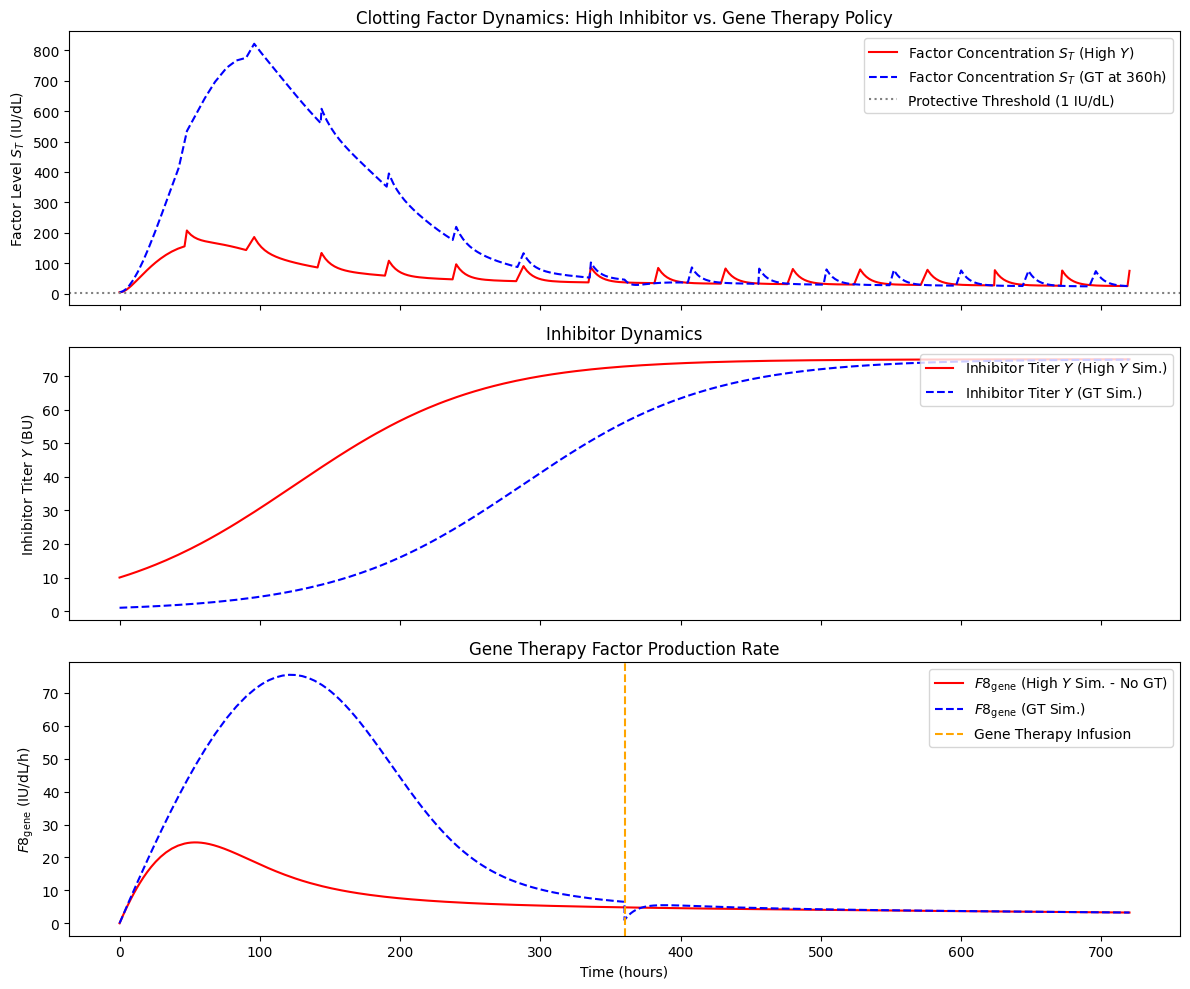
\includegraphics[width=\textwidth]{Figures/clotting_dynamics.png}
\caption{Illustrative clotting-factor dynamics under two policies. Top:
factor activity $S_T$ for a high-inhibitor infusion policy (solid) and a
gene-therapy policy (dashed) that switches to infusion at $t=360$~h. Middle:
inhibitor titre. Bottom: gene-therapy production rate. Simulated illustration,
not empirical results. Figure-generation code is not included in this archive.}
\label{fig:clotting_dynamics}
\end{figure}

\section{Summary}
\label{sec:C_summary}
Specialising the general framework to haemophilia gives a factor-kinetic model
whose small-titre limit is the classical linear model
(Proposition~\ref{prop:C_linear}), whose fixed point is stable
(Proposition~\ref{prop:C_stability}), and which exhibits a clinically meaningful
inhibitor threshold (Proposition~\ref{prop:C_threshold}); immune tolerance
induction has an extinction condition (Proposition~\ref{prop:C_iti}) and gene
therapy a closed-form equilibrium (Proposition~\ref{prop:C_gt}).

Three of these results carry a threshold: the titre at which a regimen stops
protecting, the suppression at which ITI succeeds rather than nearly succeeds,
and the inhibitor level at which gene therapy becomes uneconomic. Each is a
point at which a small change in circumstance produces a large change in
outcome, and each depends on something a health system controls rather than
something the patient's biology decides. That is the connection back to the
main argument: Mr~B's Systemic Burdens domain is not a background variable in
this model, it sits inside the equations that determine whether his treatment
works.

The eleven tests in \texttt{verification/tests/test\_haemophilia.py} assert
these results, together with the worked examples above: the steady states at
each titre, the point at which the regimen stops protecting, and the critical
suppression for immune tolerance induction. One of them asserts that a request
for a threshold under a regimen that cannot reach protection raises an error
rather than returning a number, because a silent wrong answer is the failure
mode that matters here. The computational methods are collected in
Appendix~\ref{app:computation} and the run record in
Appendix~\ref{app:verification}.


\chapter{Computational Implementation of the Dynamical Framework}
% ============================================================
% APPENDIX D -- Computational Implementation
% Reorganised: Purpose -> Relationship -> Algorithms -> Solvers ->
% Complexity -> Software -> Reproducibility -> Limitations -> Future.
% ============================================================

\label{app:computation}

\begin{ataglance}[How to read this appendix]
This appendix is about arithmetic done by machines, and it is written so that
someone else could reproduce it or show it wrong.

Two separate pieces of software are described and it matters that they are not
confused. The empirical analysis of Chapters~\ref{ch:methods}
to~\ref{ch:results2} runs in R and is the work the thesis is judged on
(\S\ref{sec:D_relationship}). The dynamical simulation of
Appendices~\ref{app:dynamical} and~\ref{app:hemo_dynamics} is a proposed future
direction and is what the algorithms and solvers here describe
(\S\ref{sec:D_algorithms}--\S\ref{sec:D_solvers}).

The remaining sections say how long the computations would take
(\S\ref{sec:D_complexity}), what would have to be recorded for another
researcher to repeat them (\S\ref{sec:D_software}), and what the present
archive does not contain (\S\ref{sec:D_limitations}). That last section is the
one to read first if the question is what has actually been built.
\end{ataglance}

\section{Purpose}
\label{sec:D_purpose}
This appendix records the computational methods that implement the dynamical
extension of Appendices~\ref{app:dynamical} and \ref{app:hemo_dynamics}, so that
the proposed future modelling can be reproduced. The algorithms below are
schematic illustrations of the dynamical simulation, not the empirical analysis
pipeline.

\section{Relationship to the Empirical Analysis}
\label{sec:D_relationship}
The empirical measurement and prognostic models of Chapters~\ref{ch:methods} to
\ref{ch:results2} are intended to be estimated in R using \texttt{lavaan} for
structural equation modelling, \texttt{survival} for the Cox models, and
\texttt{mice} for imputation \citep{vanbuuren_2011}. The V2 archive includes an executable analysis
scaffold under \texttt{analysis/}; it validates inputs and records session
information, but cannot reproduce numerical results until a documented NHATS
extract and variable mapping are supplied. The dynamical simulation described
here is separate and remains a proposed future direction, not part of the
empirical validation.

The algorithms below therefore belong to the second of those two pieces of
software. They are written out in full because a specification that cannot be
checked is not a specification.

\section{Algorithms}
\label{sec:D_algorithms}
The simulation is organised in three layers that process biomedical, stochastic,
and policy inputs in turn.

\paragraph{Algorithm 1 (biomedical and DALY calculation).}
Disability weights and the DALY construction follow \citet{gbd2019}.
Given a disease profile, life expectancy $L_0$, disability weight $w$, and
survival function $S(t)$: compute the quality index $Q$; the severity-adjusted
life expectancy $L_{\text{adj}}=L_0 Q$; the life expectancy
$\mathbb{E}[L]=\int_0^\infty S(t)\,dt$; years lived with disability
$\mathrm{YLD}=w\,\mathbb{E}[L]$; years of life lost $\mathrm{YLL}=L_0-\mathbb{E}[L]$;
$\mathrm{DALY}=\mathrm{YLD}+\mathrm{YLL}$; and biomedical potential
$BP=(L_{\text{adj}}/L_0)(1-\mathrm{DALY}/L_0)$.
The identity $\mathrm{DALY}=\mathrm{YLD}+\mathrm{YLL}$ follows directly from
the definitions above. A future reference implementation should test both this
identity and the numerical quadrature for $\mathbb{E}[L]$.

\begin{reading}[What Algorithm 1 computes, in clinical terms]
The algorithm turns a disease profile into a single number for biomedical
potential, and every step of it is standard burden-of-disease accounting.

Years of life lost is how much shorter life is expected to be than it would
otherwise have been. Years lived with disability is the remaining life weighted
by how impaired it is. Their sum is the disability-adjusted life year, which is
the currency the Global Burden of Disease study reports in.

For Mr~B the two components separate cleanly. His years of life lost are now
modest, because treatment has largely closed the survival gap that defined
haemophilia before the 1990s. His years lived with disability are substantial,
because a destroyed knee and chronic pain carry a high disability weight
for the whole of his remaining life. A measure that reported only mortality
would record him as almost unaffected, which is the reason the DALY was
invented and the reason biomedical potential is built from both terms.

The final line, $BP=(L_{\text{adj}}/L_0)(1-\mathrm{DALY}/L_0)$, rescales that
onto the unit interval the rest of the framework uses. It is a normalisation
step and carries no separate claim.
\end{reading}

\begin{workedexample}[apd-daly]{Mr~B's burden, split into its two parts}
Suppose a man of Mr~B's age would without haemophilia expect $L_0=30$ further
years, that treatment has brought his life expectancy to $\mathbb E[L]=28$
years, and that his joint damage and chronic pain carry a disability weight
$w=0.28$. Take the quality index as $Q=0.72$.

\begin{wecode}[Python]
from hpv.economics import daly, biomedical_potential

yld, yll, total = daly(L0=30.0, w=0.28, E_L=28.0)
print(f"YLD {yld:5.2f}   YLL {yll:5.2f}   DALY {total:5.2f}")
print(f"biomedical potential {biomedical_potential(30.0, 0.72, total):.4f}")

# the same man, in the era before prophylaxis reached him
yld0, yll0, total0 = daly(L0=30.0, w=0.28, E_L=15.0)
print(f"\npre-prophylaxis: YLD {yld0:5.2f}   YLL {yll0:5.2f}   "
      f"DALY {total0:5.2f}")
\end{wecode}

\noindent Today: $\mathrm{YLD}=7.84$, $\mathrm{YLL}=2.00$, so a DALY of $9.84$
of which eighty per cent is disability. In the era before prophylaxis reached
him the same weights give $\mathrm{YLD}=4.20$ and $\mathrm{YLL}=15.00$, a DALY
of $19.20$ of which seventy-eight per cent is death.

The total halved and its composition inverted. That is the whole argument for
this thesis in one calculation: a measure that tracked mortality alone would
record the modern Mr~B as almost unaffected, having correctly recorded the
1970s Mr~B as gravely affected, and would have nothing to say about the twenty
years of reduced mobility that now constitute his burden.

\weanswer{$\mathrm{DALY}=9.84$, eighty per cent of it disability, giving
$BP=0.484$. Asserted by \texttt{test\_algorithm\_one\_daly\_identity} and
\texttt{test\_worked\_example\_mr\_b\_daly\_split}.}
\end{workedexample}

The cost side of the same decision needs its own arithmetic, and the difficulty
there is not the point estimate but the interval around it.

\paragraph{Algorithm 2 (Monte Carlo cost-effectiveness).}
Draw costs and effects for two strategies, form $\Delta C$, $\Delta E$, and
$\mathrm{ICER}=\Delta C/\Delta E$; report the ratio-of-means ICER, a bootstrap
\citep{efron_tibshirani_1993} confidence interval, and the incremental net
monetary benefit at a willingness-to-pay threshold \citep{briggs_2006}. Recovery of a planted ICER with a bracketing
interval should be verified by a unit test before a numerical result is reported.

\begin{reading}[Why an ICER needs a bootstrap and not a formula]
The incremental cost-effectiveness ratio is a ratio of two uncertain
quantities, and ratios misbehave. When the denominator $\Delta E$ is small and
its confidence interval crosses zero, the ratio's interval is not an interval
at all: it covers everything except a finite middle region, and the usual
standard-error formula returns a number that means nothing.

The clinical intuition is the same one behind a relative risk computed on three
events. The point estimate looks precise and the ratio is unstable because the
denominator is nearly nothing.

This is why the net monetary benefit is reported alongside. Rearranging
$\lambda\Delta E-\Delta C$ removes the division and gives a quantity whose
uncertainty behaves, at the cost of requiring the threshold $\lambda$ to be
named rather than left implicit in a ratio. Naming it is an improvement, not a
concession.
\end{reading}

Both algorithms assume the underlying differential equations can be integrated
accurately. That is a property of the solver rather than of the model, and it
has to be demonstrated rather than assumed.

\section{Numerical and Stochastic Solvers}
\label{sec:D_solvers}
\begin{itemize}
  \item \textbf{Deterministic.} Explicit Runge--Kutta 4(5) \citep{butcher_2008} for ODEs, with stiff
  variants (Radau, BDF) invoked adaptively; a fixed-step RK4 is used where the
  step count must be controlled.
  \item \textbf{Stochastic.} Euler--Maruyama and Milstein schemes \citep{kloeden_platen_1992} for
  $dX=f\,dt+g\,dW_t$; the Milstein correction raises the strong order to one.
  \item \textbf{Population diffusion PDE.} Conservative finite-volume assembly
  with an implicit (backward-Euler / Crank--Nicolson) time step; alternating-
  direction implicit schemes generalise this to higher dimensions.
\end{itemize}
For a sufficiently smooth problem in the asymptotic regime, fourth-order RK4
should show an error ratio approaching $16$ under step halving; this is a
recommended verification test rather than a result established in this archive.

\begin{reading}[What the order-of-convergence test actually checks]
Halve the step size and the error of a method of order $q$ should fall by a
factor of $2^q$: sixteen for a fourth-order scheme, thirty-two for a
fifth-order one. The embedded Dormand--Prince pair used here advances at fifth
order and carries a fourth-order estimate for step control, so the ratio to
look for depends on which solution is propagated, and the test has to state
which. Observing the predicted ratio is the standard way to show that a solver
is doing what it claims.

It is worth being clear about what the test does and does not establish. It
checks the arithmetic, not the biology. A solver can integrate a wrong equation
to machine precision, and the convergence test will pass. Passing it means the
numbers in a figure are the numbers the model implies; it does not mean the
model implies anything true about a patient.

The distinction matters here because the dynamical appendices make no empirical
claims. Their whole content is that certain equations have certain properties,
and a solver that fails this test would leave even that unestablished.
\end{reading}

\begin{workedexample}[apd-order]{Running the convergence test rather than asserting it}
The claim is that halving the step cuts a fourth-order method's error by
sixteen. The way to establish it is to run it. Integrate the deterministic
model of Appendix~\ref{app:dynamical} from a fixed start over four time units
with fixed-step RK4, taking a very fine run as the reference.

\begin{wecode}[Python]
from hpv.dynamics import integrate_ode

P = dict(Vmax=100.0, Km=10.0, T=20.0, k_inh=0.05, Y=2.0,
         gamma=30.0, Kd=50.0, n=2.0, Z=80.0, k_elim=0.8)
ref = integrate_ode(0.0, 4.0, P, dt=1e-5)

prev = None
for dt in (0.4, 0.2, 0.1, 0.05):
    err = abs(integrate_ode(0.0, 4.0, P, dt=dt) - ref)
    ratio = "" if prev is None else f"   ratio {prev / err:5.2f}"
    print(f"dt {dt:<5} error {err:.3e}{ratio}")
    prev = err
\end{wecode}

\noindent Errors of $1.83\times10^{-3}$, $9.81\times10^{-5}$,
$5.68\times10^{-6}$ and $3.42\times10^{-7}$, giving ratios of $18.61$, $17.25$
and $16.61$. The ratios approach sixteen from above as the step shrinks, which
is what fourth-order convergence looks like in practice: the asymptotic rate is
reached from the direction of the higher-order terms that dominate at coarse
steps.

Two cautions belong with this. A ratio near sixteen shows the integrator is
solving the equation it was given to the order it claims; it says nothing about
whether that equation describes a patient. And the reference run is itself
numerical, so the last row is measuring the coarse run against a fine run
rather than against the truth; the test stops refining before that distinction
starts to matter.

\weanswer{Error ratios of $18.61$, $17.25$ and $16.61$ under successive step
halving, approaching the fourth-order value of $16$ from above. Asserted by
\texttt{test\_worked\_example\_apd\_order\_of\_convergence}.}
\end{workedexample}

Accuracy settled, the remaining practical question is whether the computations
finish in reasonable time.

\begin{lstlisting}[language=Python,basicstyle=\footnotesize\ttfamily,frame=single]
import numpy as np
from scipy.integrate import solve_ivp

def disease_model(t, y, params):
    X = y[0]
    Vmax, Km, k_inh, Kd, n, k_elim, Y, Z, T = params
    f = Vmax * T / (Km + T)          # Michaelis-Menten treatment
    g = k_inh * Y * X                # bilinear inhibition
    h = Z**n / (Kd**n + Z**n)        # Hill stabilisation
    return [f - g + h - k_elim * X]

sol = solve_ivp(disease_model, [0, 100], [1.0], args=(params,), method='RK45')
\end{lstlisting}

\section{Computational Complexity}
\label{sec:D_complexity}
The cost of each solver scales as follows, with $n$ time steps, $N$ paths, $M$
Monte Carlo draws, and $(n_x,n_t)$ the space and time resolution of the PDE.
\begin{center}
\begin{tabular}{ll}
\toprule
Component & Complexity \\
\midrule
ODE (RK4, 4 evaluations per step) & $O(n)$ \\
SDE (Euler--Maruyama, $N$ paths)  & $O(nN)$ \\
Monte Carlo ($M$ draws)           & $O(MN)$ \\
PDE (Fokker--Planck, sparse solve)& $O(n_x n_t)$ \\
\bottomrule
\end{tabular}
\end{center}
For a fixed-step implementation, RK4 uses $4n$ right-hand-side evaluations and
Euler--Maruyama updates $nN$ path--time cells. These counts should be asserted in
unit tests when the future simulation package is implemented.

The table has one line worth noticing. The single-patient ODE costs $O(n)$ and
the population Fokker--Planck solve costs $O(n_xn_t)$, so following a whole
cohort as a density is cheaper than simulating enough individual paths to
estimate the same distribution. That is the practical argument for the
population layer of Appendix~\ref{app:dynamical}, alongside the conceptual one.

What none of these costs include is the work of making a computation
reproducible by someone else, which is where most of the effort in practice
goes.

\section{Software and Reproducibility}
\label{sec:D_software}
The proposed dynamical implementation would use NumPy for arrays, SciPy for
integration and linear algebra, and optionally Numba for performance-critical
loops. Reproducibility requirements are a fixed random seed, a locked software
environment, machine-readable parameters, unit tests for limiting cases and
convergence, and scripts that regenerate every reported figure. These are design
requirements, not claims about software included in the present archive.

That last sentence is the honest position, and the next section states its
consequences plainly rather than leaving them to be inferred.

\section{Limitations and Future Implementation}
\label{sec:D_limitations}
The code is a reference implementation of a proposed modelling direction, not a
clinical tool: parameters are illustrative, no patient data is used, and the
population layer is one-dimensional. Future work would calibrate parameters to
longitudinal factor-level data, extend the PDE to several biomarkers, and couple
the dynamical state to the validated latent score through the time-varying form
of Appendix~\ref{app:dynamical}.

\section{Summary}
\label{sec:D_summary}
This appendix collected the algorithms, solvers, complexity, and reproducibility
requirements for the dynamical models of Appendices~\ref{app:dynamical} and
\ref{app:hemo_dynamics}. It is deliberately separate from the empirical R
pipeline of the main text. No claim of machine verification is made until the
future simulation implementation and its tests are deposited with the thesis.


\chapter{Verification: the Code That Asserts the Results}
% ============================================================
% APPENDIX F -- Verification: the code that asserts the results
% ============================================================

\label{app:verification}

\begin{ataglance}[How to read this appendix]
Every numbered result in this thesis that can be checked by computation is
checked by computation, and this appendix is the record.

\S\ref{sec:F_why} says what the suite does and, more importantly, what it does
not do: it verifies mathematics, not medicine, and passing it is not evidence
about any patient. \S\ref{sec:F_arch} describes the reference implementation
and the naming rule that ties one test to one numbered statement.
\S\ref{sec:F_run} says how to run it. \S\ref{sec:F_results} prints the outcome
of the run that produced this copy of the thesis. \S\ref{sec:F_found} records
the two errors the suite caught, because a verification appendix that reports
only successes is a marketing document. \S\ref{sec:F_limits} sets out what
remains unverified and why.
\end{ataglance}

\section{What the Suite Is For, and What It Cannot Do}
\label{sec:F_why}

A proof establishes that a statement follows from its premises. It does not
establish that the statement was transcribed correctly into the thesis, that
the arithmetic in a worked example is right, or that the implementation someone
later writes computes the object the proof was about. Those are different
failures, they are common, and they are the ones a test suite catches.

The suite here does four things. It checks that each stated property holds for
the implemented function across a grid of inputs, which catches a
transcription error in a formula. It checks that each worked example in the
text returns the number the text prints, which catches arithmetic slips and,
more usefully, catches them again whenever a parameter is later edited. It
checks the internal consistency of the running cases, so that Mrs~A's realised
capability is the same figure in Chapter~\ref{ch:theory} and in
Chapter~\ref{app:crf}. And it checks the qualitative claims the prose makes
about the mathematics, such as that lowering the substitution parameter
punishes imbalance harder, which are the claims most easily asserted and least
often verified.

What it does not do needs stating plainly, because verification suites attract
more credit than they deserve.

\begin{itemize}
\item \textbf{It is not a proof.} A property that holds on a finite grid of
inputs may fail elsewhere. The proofs are in
Appendix~\ref{app:mathematical_foundations} and Chapter~\ref{app:crf}; the tests check
that the implementation agrees with them, which is a weaker and different
claim.

\item \textbf{It is not empirical validation.} No participant data are used.
Nothing here says whether the three domains exist, whether the indicators
measure them, or whether the construct predicts anything. Those questions
belong to Chapters~\ref{ch:results1} and~\ref{ch:results2} and are answered by
data, not by assertions in Python.

\item \textbf{It cannot check the axioms.} Whether capacity boundedness is the
right commitment, or whether $\varepsilon$ should be $0$ or $2$, are questions
no test can settle. The suite verifies that the mathematics does what the
axioms say; it is silent on whether the axioms are correct.

\item \textbf{Passing is not a quality claim.} A suite tests what its author
thought to test. Its value lies in what it caught, which
\S\ref{sec:F_found} reports, and in the fact that it will catch the same class
of error again when the thesis is next edited.
\end{itemize}

The honest summary is that this appendix raises confidence in the
\emph{bookkeeping} of a long mathematical argument. That is worth having. It is
not worth more than it is.

\section{Architecture and the Naming Rule}
\label{sec:F_arch}

The code lives in \texttt{verification/} in the thesis archive and has two
parts. The package \texttt{hpv} is a reference implementation: one module per
mathematical layer, with every function carrying the number of the result it
implements. The directory \texttt{tests/} holds the assertions.

\begin{table}[htbp]\centering
\caption{The reference implementation. Each module implements the objects of
one mathematical layer of the thesis.}
\label{tab:F_modules}
\footnotesize
\begin{tabular}{p{3.4cm} p{2.4cm} p{7.6cm}}
\toprule
\textbf{Module} & \textbf{Source} & \textbf{Objects implemented} \\
\midrule
\texttt{hpv/crf.py} & App.~\ref{app:mathematical_foundations}, Ch.~\ref{app:crf} &
Domain profile, CES contextual mean and its geometric limit, the additive and
relational comparators, deprivation counting, gradients and elasticities,
cross-partials, the gap decomposition, the Atkinson equally distributed
equivalent and its social weights \\
\addlinespace
\texttt{hpv/dynamics.py} & App.~\ref{app:dynamical} &
Michaelis--Menten and Hill terms, the drift of the deterministic model, its
closed-form equilibrium, the Lipschitz constant, fixed-step RK4,
Euler--Maruyama, and a conservative finite-volume Fokker--Planck step \\
\addlinespace
\texttt{hpv/haemophilia.py} & App.~\ref{app:hemo_dynamics} &
Neutralisation fraction, the factor steady state, the inhibitor threshold, the
linear reference model, the ITI equilibrium and its critical suppression, the
gene-therapy equilibrium \\
\addlinespace
\texttt{hpv/economics.py} & App.~\ref{app:a-economics}, \ref{app:computation} &
Net health benefit, incremental net monetary benefit, displaced health, budget
impact, discounting, the ICER, and the DALY identity \\
\addlinespace
\texttt{hpv/prognostic.py} & Ch.~\ref{ch:methods}, \ref{ch:results2} &
Hazard-ratio to absolute-risk conversion, cumulative incidence under a
competing risk against the Kaplan--Meier complement, decision-curve net
benefit, and classical-error attenuation \\
\bottomrule
\end{tabular}
\end{table}

The naming rule is the part that makes the suite usable rather than
decorative. Every test function is named for the statement it asserts:
\texttt{test\_proposition\_inhibitor\_threshold},
\texttt{test\_theorem\_gap\_decomposition\_is\_exact},
\texttt{test\_worked\_example\_mrs\_a\_absolute\_risk}. A reader who doubts
Proposition~\ref{prop:C_threshold} can find the test that asserts it by name,
read the assertion, and change the numbers. Every test carries a docstring
naming the result and saying in one sentence what would be wrong if it failed.

This is also why the pointer beneath each proposition in the appendices reads
\emph{Verified numerically by} and then a test name. In the previous version of
this thesis those pointers named tests in a package called \texttt{volos} that
did not exist. Announcing a verification engine one has not written is worse
than writing nothing, and the pointers now name tests that run.

\section{Running the Suite}
\label{sec:F_run}

The suite needs Python 3.10 or later, \texttt{pytest} and \texttt{numpy}, and
nothing else. From the \texttt{verification/} directory:

\begin{lstlisting}[style=hpcode,language=bash]
pip install pytest numpy
python3 -m pytest tests/ -q          # run everything
python3 -m pytest tests/ -q -k threshold   # run one result
python3 run_verification.py          # run everything and write the table below
\end{lstlisting}

\noindent
The runner writes two files. \texttt{verification\_results.tex} is the table in
\S\ref{sec:F_results}, regenerated on every build, so the table cannot drift
away from the code that produced it. \texttt{verification\_results.json} is the
same record in machine-readable form, with the timestamp, the Python version
and the platform, so a reader can tell whether the printed table came from the
code they are holding.

Stochastic tests fix their seeds. The Monte Carlo comparisons use tolerances
set from the standard error of the estimator rather than tuned until they
passed, and the seeds are declared in the source so a failure can be
reproduced.

\section{Results of the Run That Produced This Document}
\label{sec:F_results}

% Generated by verification/run_verification.py. Do not edit by hand.
\begin{table}[htbp]\centering
\caption{Result of running the verification suite. Each test asserts a numbered statement from the chapter or appendix named. The suite is re-run and this table regenerated on every build of the thesis.}
\label{tab:verification}
\footnotesize
\begin{tabular}{p{4.6cm} p{1.6cm} p{5.4cm} r r}
\toprule
\textbf{Test module} & \textbf{Covers} & \textbf{Subject} & \textbf{Passed} & \textbf{Failed} \\
\midrule
\texttt{test\_axioms.py} & A & Axioms, aggregation and the rival ontology & 39 & 0 \\
\texttt{test\_crf.py} & E & Capability Realisation Function & 19 & 0 \\
\texttt{test\_dynamics.py} & B & Dynamical layers: ODE, SDE, Fokker--Planck & 14 & 0 \\
\texttt{test\_haemophilia.py} & C & Factor kinetics, ITI and gene therapy & 11 & 0 \\
\texttt{test\_economics.py} & A, D & Net benefit, budget impact and DALYs & 10 & 0 \\
\texttt{test\_prognostic.py} & 3, 6 & Survival, competing risks and net benefit & 16 & 0 \\
\texttt{test\_measurement.py} & 5 & Reliability, validity and factor scores & 10 & 0 \\
\texttt{test\_chapter\_examples.py} & 1, 7--9 & Worked examples in the chapters & 7 & 0 \\
\midrule
\textbf{Total} & & & \textbf{126} & \textbf{0} \\
\bottomrule
\end{tabular}
\end{table}

\noindent\emph{Run 2026-09-03 11:58 UTC on Python 3.11.15, Linux-6.18.44-fc-v24-x86\_64-with-glibc2.39, in 30.1\,s.}


\noindent
A failing row would appear here, in this table, in the submitted thesis. That
is the intention. A verification appendix whose table is generated by the same
command that builds the document cannot quietly report a state of affairs that
has ceased to be true.

\section{What the Suite Caught}
\label{sec:F_found}

Two errors surfaced on the first runs. Both are recorded because the value of a
test suite is measured in what it finds, and because both are instructive about
what kinds of checking catch what kinds of mistake.

\subsection{A worked example that proved nothing}

The compensation example in \S\ref{app:a-additivity} was written with Mr~B's
structural freedom falling from $0.20$ to $0.05$ while immune tolerance
induction raised his biomedical potential from $0.30$ to $0.60$. The additive
index scores the change as an improvement, which was the point. The realisation
function was supposed to score it as a deterioration, and does not: both
profiles return exactly $0.112$, because
$0.60\sqrt{0.70\times0.05}$ and $0.30\sqrt{0.70\times0.20}$ are the same
number. The example demonstrated a difference between the two rules that, at
those particular numbers, did not exist.

The parameter was changed to $0.04$, where the realisation function returns
$0.100$ against $0.112$ and the two rules disagree about the sign of the
change. The point survives; the arithmetic that was supposed to carry it now
does.

The general lesson is that a hand-worked example is a piece of evidence, and
like any piece of evidence it can be checked or taken on trust. This one had
been read several times by a human and the coincidence was not noticed.

\subsection{A sign error that mass conservation could not see}

The finite-volume Fokker--Planck step in \texttt{hpv/dynamics.py} was written
with the advective flux entering the assembled operator with the wrong sign, so
a positive drift moved the population density towards lower biomarker values
instead of higher ones.

The interesting part is which test failed. The mass-conservation test of
Proposition~\ref{prop:B_mass} passed throughout, both before and after the
correction, because a sign error in the flux still leaves the operator's column
sums at zero: probability was conserved perfectly while flowing the wrong way.
Only the test asserting that drift moves the mean and diffusion widens the
variance, which is the qualitative claim the prose in \S\ref{sec:B_fp} makes,
caught it.

Conservation properties are the natural thing to test in a discretised
transport problem, and they are insensitive to direction. A suite built only
from the invariants a numerical analyst would think to check would have shipped
this. The test that caught it was written to verify a sentence in the
manuscript rather than a property of the scheme, which is an argument for
writing tests from the prose as well as from the mathematics.

\section{What Remains Unverified}
\label{sec:F_limits}

Three classes of claim in this thesis are not covered, and it is better to name
them than to let the table above imply a coverage it does not have.

\textbf{Everything that needs data.} The measurement model, the factor
structure, the invariance tests, the survival models and every performance
statistic in Chapters~\ref{ch:results1} and~\ref{ch:results2} require the NHATS
extract, which is not part of this archive. The R scripts under
\texttt{analysis/} validate their inputs and record session information but
cannot reproduce a numerical result until a documented extract and variable
mapping are supplied. What the Python suite covers on the prognostic side is
the arithmetic of hazard conversion, competing risks, net benefit and
attenuation, which is the part that can be checked without a cohort.

\textbf{The proofs themselves.} No theorem prover is used. The tests check
agreement between the implementation and the stated result on sampled inputs;
they cannot establish that a proof is valid, and a reader who doubts a proof
should read the proof.

\textbf{The normative content.} The axioms, the choice of $\alpha$, the range
of $\rho$, the value of $\varepsilon$ and the opportunity-cost threshold
$\lambda$ are judgements. The suite verifies what follows from a given choice.
It has nothing to say about whether the choice is defensible, and no amount of
green output should be read as though it did.




% =========================================================
% References
% =========================================================
\cleardoublepage
\addcontentsline{toc}{chapter}{References}
\bibliographystyle{agsm}
\bibliography{refs}

\end{document}
